% Create a one-sided article document type
\documentclass[a4paper, twoside, 12pt]{book}

% Define the course variables that are gonna be used several times
\newcommand{\university}{Universidad\ Politécnica\ de\ Madrid}
\newcommand{\school}{Departamento de Inteligencia Artificial \protect\\
                     Escuela\ Técnica\ Superior\ de\ Ingenieros Informáticos}
\newcommand{\degree}{}    
\newcommand{\name}{Towards Explainable Machine Learning for Anomaly Detection in Real-World Contexts}
\newcommand{\tfm}{PhD \ Thesis}
\newcommand{\nameShort}{Towards Explainable Machine Learning for Anomaly Detection}

\newcommand{\me}{Alberto Barbado González}
\newcommand{\supervisor}{Dr. Óscar Corcho}

% Configure the metadata of the PDF document
\usepackage[
	bookmarks       = true,             % Show the bookmarks
	unicode         = true,             % Use Unicode                 
	pdftoolbar      = true,             % Show Acrobat’s toolbar
	pdfmenubar      = true,             % Show Acrobat’s menu
	pdffitwindow    = false,            % Window fit to page when opened
	pdfstartview    = {FitH},           % Fit the page width to the window
	pdfauthor       = {\me},            % The author of this document
	pdftitle        = {\name\ --\ \me}, % The title of this document
	pdfsubject      = {\name},          % The subject of this document
	pdfkeywords     = {\name},          % The keywords of this document
	pdfnewwindow    = true,             % Open the links in a new PDF window
	colorlinks      = true,             % Use colored links
	linkcolor       = blue,             % Internal links color
	citecolor       = blue,             % Bibliographic links color
	filecolor       = cyan,             % File links color
	urlcolor        = magenta           % External links color
]{hyperref}

% Redefine the size and margins (delete the 'twoside' indentation)
\usepackage[a4paper]{geometry}
% Define the geometry of the document
\newgeometry {
    top = 2.2cm, 
    bottom = 2.2cm, 
    right = 2cm, 
    left = 2cm
}
% Use UTF-8 as input encoding
\usepackage[utf8]{inputenc}
% Use a modern font (that is not pixelated)
\usepackage{lmodern}
% Use microtype to improve readability
\usepackage[protrusion = true, expansion = true]{microtype} 
% Use multiple columns
\usepackage{multicol}
% Display two figures next to each other
\usepackage{subfigure}
\usepackage[subfigure]{tocloft}
% Display list of Equations
\usepackage{tocloft}
% Insert empty pages
\usepackage{afterpage}
% Configure style aspects of the document
\usepackage{caption}            % To configure the captions
\usepackage{siunitx}            % For SI units
\usepackage{graphicx}           % To include graphics
\usepackage[dvipsnames]{xcolor} % To configure colors
\usepackage{fancyhdr}           % To configure the header and footer
\pagestyle{fancy}               % Use a fancy header style
\fancyhf{}                      % Set the header format
\fancyheadoffset{0.0 cm}        % Set the header offset
\lhead{\tfm}                    % Set the header right-side contents
\rhead{\nameShort}              % Set the header left-side contents
\cfoot{\thepage}                % Set the footer page number

% Additional Packages
%\usepackage[backend=biber,style=numeric,sorting=none]{biblatex}
\usepackage[
    backend=biber,
    style=apa, 
    sorting=nyt,
    maxbibnames=999,
    maxcitenames=2,
    mincitenames=1
    ]{biblatex}
\usepackage{xcolor, colortbl}
\usepackage{mathtools}
\usepackage{algorithm}
\usepackage{algpseudocode}
\usepackage{tocbibind}
\usepackage{tocloft}
\usepackage{xpatch}
\usepackage{array,booktabs}
\usepackage{makecell}
\usepackage{pdfpages}
\DeclareUnicodeCharacter{0301}{}
\usepackage[T1]{fontenc}


% Add hyperref
\usepackage{hyperref}

%\usepackage[usenames,dvipsnames]{xcolor} % TODO: LO QUITO PORQUE CREO QUE NO HACE NADA
\usepackage[breakable, theorems, skins]{tcolorbox}
\tcbset{enhanced}

\newcommand*\rot{\rotatebox{90}}

% Color boxes
\DeclareRobustCommand{\mybox}[2][gray!20]{%
\begin{tcolorbox}[   %% Adjust the following parameters at will.
        breakable,
        left=0pt,
        right=0pt,
        top=0pt,
        bottom=0pt,
        colback=#1,
        colframe=#1,
        width=\dimexpr\textwidth\relax, 
        enlarge left by=0mm,
        boxsep=5pt,
        arc=0pt,outer arc=0pt,
        ]
        #2
\end{tcolorbox}
}


%\usepackage{rotating}
\usepackage[counterclockwise, figuresleft]{rotating}
\addbibresource{main.bib}

% Create a custom command shortcut
\renewcommand{\arraystretch}{1.3} % Modify the vertical spacing of the tables
\raggedbottom                     % Modify the vertical spacing of enumerated environments

% Set empty page 
\newcommand\blankpage{%
    \null
    \thispagestyle{empty}%
    \addtocounter{page}{-1}%
    \newpage
}

\newcommand{\fontnormal}{\fontsize{14 pt}{12 pt}\selectfont}

% Set the title format
\title {
	\vspace*{1.0 cm}
	\Large\textbf{\uppercase{\university}} \\
	\vspace*{0.5 cm}
	\large\textbf{\uppercase{\school}} \\
	%\rule{470 pt}{2 pt} \\ %380
	\vspace*{2 cm}
	\LARGE\textbf{\uppercase{\name}} \\
	%\rule{470 pt}{2 pt} \\
	\vspace*{2 cm}
	%\large\text{\uppercase{\degree}} \\

    \vspace*{0.5 cm}
	\large\text{\uppercase{\tfm}} \\
	\vspace*{2.0 cm}
	
	\normalsize
	\begin{tabbing}
        \hspace*{0.4\linewidth} \= \hspace*{0.5\linewidth} \= \kill
    	\> Author: \' \textbf{\me} \\[0.25cm]
    	\> Supervisor: \' \textbf{\supervisor} \\
    	\> Supervisor: \' \textbf{Dr. Richard Benjamins} \\
    \end{tabbing}
    
    \vspace*{1 cm}
    
    %\parbox{\linewidth}{
    %   \centering%
    %   \fontnormal%
    %   A thesis submitted in fulfilment of the requirements \protect\\
    %   for the degree of Doctor of Philosophy \protect\\
    %   in the \protect\\
    %   Escuela Técnica Superior de Ingenieros Informáticos \protect\\
    %   Departamento de Inteligencia Artificial}
    %   }

}

% Set the author format [NOT USED]
\author {
	\normalsize
	\begin{tabbing}
        \hspace*{0.4\linewidth} \= \hspace*{0.5\linewidth} \= \kill
    	\> Author: \' \textbf{\me} \\[0.25cm]
    	\> Supervisor: \' \textbf{\supervisor} \\
    	\> Supervisor: \' \textbf{\author} \\
    \end{tabbing}
    
    \vspace{2cm}
}

% Set the date format
\date { 
    December, 2022
}

% A macro to print the title
\makeatletter
\def\printtitle{{\centering\@title\par}}
\makeatother

% A macro to print the author
\makeatletter
\def\printauthor{{\centering\large\@author}}
\makeatother

% A macro to print the date
\makeatletter
\def\printdate{{\centering\@date}}
\makeatother

%%%%%%%%%%%%%%%%%%%%%%%%%%%%%%%%%%%%%%%%%%%%%%%%%%%%%%%
% Start the document
\begin{document}
    % Include the cover
    \afterpage{\blankpage}
    %

\thispagestyle{empty}

%\usepackage{pdfpages}
%
\includepdf{includes/initial_sections/diapo_cubierta.pdf}


\newpage
    
\includepdf{includes/initial_sections/diapo_cubierta.pdf}
    \thispagestyle{empty} % Remove page numbering on this page

\begin{center}
    
    \centering
    \begin{figure}[h!]
        \centering
        \begin{subfigure}
            \centering
            % Include UPM's logo
        	
\includegraphics[width = 0.5\linewidth, height = 3cm, keepaspectratio]{images/UPM.eps}
    	\end{subfigure}
    	\hspace{3cm}%
    	\centering
        \begin{subfigure}
            \centering
            % Include ETSII's logo
        	
\includegraphics[width = 0.5\linewidth, height = 3cm, keepaspectratio]{images/ETSII.eps}
        \end{subfigure}
	\end{figure}
	
	% Print the title
	\printtitle
	
	% Add vertical padding
    \vfill
    
    % Print the author
    %\printauthor
    
    % Print the date
    \printdate
\end{center}

\newpage              % Insert a page break
\setcounter{page}{1}  % Set the page counter
    
    % Initial Sections
    \thispagestyle{empty}
\topskip0pt
\vspace*{8em}

Tribunal nombrado por el Sr. Rector Magfco. de la Universidad Politécnica de Madrid,
el día ...... de ................ de ..........
\newline\newline

Presidente:\newline

Vocal:\newline

Vocal:\newline

Vocal:\newline

Secretario:\newline

Suplente:\newline

Suplente:\newline\newline

Realizado el acto de defensa y lectura de la Tesis el día ...... de ................ de ..........
en la Escuela Técnica Superior de Ingenieros Informáticos.\newline\newline

Calificación: \rule{333 pt}{0.5 pt}\newline\newline\newline\newline

{\centering
  EL PRESIDENTE \hspace{30 mm} VOCAL 1 \hspace{30 mm} VOCAL 2\par
}
\vspace{35mm}
{\centering
  VOCAL 3  \hspace{40 mm} EL SECRETARIO\par
}

\newpage

    \tableofcontents

\newpage
    {%
    \let\oldnumberline\numberline%
    \renewcommand{\numberline}{Figure~\oldnumberline}%
    \vspace{1cm}
    \listoffigures%
}

\phantomsection
%\addcontentsline{toc}{chapter}{List of Figures}

\newpage
    {%
    \let\oldnumberline\numberline%
    \renewcommand{\numberline}{Table~\oldnumberline}%
    \listoftables%
}


\phantomsection
%\addcontentsline{toc}{chapter}{List of Tables}
\pagebreak
    {%
    \let\oldnumberline\numberline%
    \renewcommand{\numberline}{Algorithm~\oldnumberline}%
    \vspace{1cm}
    \listofalgorithms%
}

\phantomsection
\pagebreak
    


\newcommand{\listequationsname}{List of Equations}
\newlistof{myequations}{equ}{\listequationsname}
\newcommand{\myequations}[1]{%
\addcontentsline{equ}{myequations}{\protect\numberline{\theequation}#1}\par}
\setlength{\cftmyequationsnumwidth}{2.5em}% Width of equation number in List of Equations

\listofmyequations


    
    \topskip0pt
\vspace*{15em}

%\begin{center}
\chapter*{Abstract}

    % Opcion (I)
    %Anomaly detection is a crucial task within many industry applications, from discovering fraudulent credit card transactions to detecting faults within mechanical system. The reason is that it can find patterns in data that do not follow the expected behaviour.
    
    % Opcion (II): Importance anomaly detection + Unsupervised ML
    Anomaly detection is a crucial task within many real-world applications since it can find patterns in data that do not follow the expected behaviour. Consequently, it serves for addressing different business problems, from discovering fraudulent credit card transactions to detecting faults within mechanical systems. Among the different approaches for detecting anomalies within large amounts of data, unsupervised techniques, especially \textit{unsupervised Machine Learning} (ML), are particularly useful because there is normally a scarcity of labelled anomalies, hindering the usage of supervised methods.
    
    % Problem with using only binary outputs + XAI
    Many of those unsupervised methods are black boxes that only provide a binary output, lacking explanation about the factors behind the model's decision. A solution for solving this issue is the usage of \textit{Explainable Artificial Intelligence} (XAI) techniques. One of the aims of XAI is enabling humans to understand a model's decision. However, most of the research on XAI deals with supervised models. Hence, there is a need of additional research for the usage of XAI, in general, and for explaining unsupervised anomaly detection models in particular.
    
    % Problems with XAI: Metrics & Domain Knowledge
    Nevertheless, there are several XAI methods that can be considered for this purpose, and it is not trivial to compare them for finding the best one to choose for a specific use case. This highlights the need for XAI-specific metrics that can quantitatively measure different aspects of the quality of the explanations that have been generated. Another limitation is that XAI can provide explanations that contradict prior domain knowledge, leading to potentially misleading or incorrect conclusions. This leads to the research problems studied within this thesis.
    %The reason is that the patterns that are inferred form the available data may not account for causality aspects.

    % Proposal: Metrics for rule-extraction and feature relevance methods
    % Real use cases: comms and fleet. Comms proposal, fleet proposal
    In the first part of the thesis, we work with rule extraction-based techniques applied to unsupervised ML algorithms for anomaly detection. We propose two metrics, \textit{stability} and \textit{diversity}, for measuring the quality of the explanations, along with other metrics. We also include two new algorithmic variations of an already-existing post-hoc XAI technique for rule extraction. This leads to an end-to-end framework for generating and explaining anomalies from unsupervised ML algorithms, which has been published as an open-source library.
    
    After that, we study the applicability of XAI for explaining anomalies within real-world industry contexts. First, we analyse it within the context of telecommunications data, where we propose an algorithm for generating visual and counterfactual explanations for unsupervised ML algorithms for anomaly detection. The algorithm includes prior domain knowledge during the phase for searching hyperparameter combinations that not only have a good model performance, but also generate explanations that are aligned with that prior knowledge. 
    
    Then, we study XAI for explaining fuel anomalies of diesel and petrol vehicles. We propose an approach for generating explanations that identify vehicles with anomalous fuel consumption, the potential causes behind them, and the impact that those anomalies have on the fuel usage. These explanations are used for generating fuel saving recommendations that are adjusted depending on two different user profiles that will use them: fleet managers and fleet operators. The proposal includes an evaluation with XAI-specific metrics, and the combination of XAI techniques with prior domain knowledge for both explanation generation and metric evaluations. 
    
    Our work is relevant at a scientific, industry and business level: we have published two papers that are already cited, there are two patents associated to our proposals, and these proposals are already part of software products deployed to production.
    
%\end{center}


\phantomsection
\addcontentsline{toc}{chapter}{Abstract}

\newpage
    \topskip0pt
\vspace*{15em}

%\begin{center}
\chapter*{Resumen}
Detectar anomalías es crucial en muchas aplicaciones industriales debido a que se pueden encontrar patrones en los datos que no siguen un comportamiento esperado. Así, sirve para abordar distintos problemas de negocio, desde el descubrimiento de transacciones fraudulentas a la detección de fallos dentro de un sistema mecánico. Dentro de las soluciones para detectar anomalías en grandes volúmenes de datos destacan las de Aprendizaje Automático (ML) no supervisado, especialmente cuando no se dispone de información previas sobre dichas anomalías.

Muchas de esas técnicas son "cajas negras" que no incluyen sin explicaciones sobre factores detrás de la decisión del modelo. Una solución para solventarlo es la Inteligencia Artificial Explicable (XAI). Con XAI se ayuda a qué el ser humano entienda la decisión que ha tomado el modelo. Sin embargo, la mayor parte de la investigación sobre XAI se ha centrado en modelos de ML supervisados, existiendo un ámbito por explorar sobre los modelos no supervisados en general, y particularmente en el caso de los de detección de anomalías.

Existen distintas técnicas de XAI que se pueden considerar para este propósito y no es trivial ver cómo poderlas comparar para elegir la mejor para cada caso de uso específico. Esto resalta la necesidad de disponer de métricas de XAI que sirvan para poder medir, de manera cuantitativa, distintos aspectos relacionados con las explicaciones que se han generado. Otra limitación es que las técnicas de XAI pueden generar explicaciones que contradigan el conocimiento a priori del dominio, lo que puede llevar a dar información potencialmente engañosa o a tomar conclusiones erróneas. Esto conduce a los problemas de investigación estudiados en esta tesis.

En la primera parte de la tesis se trabaja con técnicas basadas en la extracción de reglas aplicadas a
algoritmos de ML no supervisados para la detección de anomalías. Proponemos dos métricas, estabilidad y
diversidad, para medir la calidad de las explicaciones. También proponemos dos algoritmos basados en una técnica post-hoc de XAI ya existente para la extracción de reglas. Esto conduce a una solución integral para generar y explicar anomalías sobre de algoritmos ML no supervisados, publicado como una librería de código abierto.

Después estudiamos las técnicas de XAI para explicar anomalías en contextos industriales reales. Primero, lo analizamos dentro del contexto de los datos de telecomunicaciones, proponiendo un algoritmo para generar explicaciones visuales y contrafactuales para ML no supervisado para detección de anomalías. Nuestro algoritmo incluye conocimiento previo del dominio durante la fase de búsqueda de hiperparámetros no sólo considerando un buen rendimiento del modelo, sino también el que las explicaciones estén alineadas con ese conocimiento previo.

Tras ello, estudiamos el uso de XAI para explicar anomalías de combustible de vehículos. Proponemos una metodología para generar explicaciones que identifiquen vehículos con consumo anómalo de combustible, las causas detrás de ello y el impacto que esas anomalías tienen en el uso de combustible. Estas explicaciones generarán recomendaciones de ahorro de combustible ajustadas para dos perfiles diferentes: gestores de flotas y operadores de flotas. La propuesta incluye una evaluación con métricas específicas de XAI, y la combinación de XAI con conocimiento previo del dominio para la generación de explicaciones y para la evaluación de métricas.

Nuestro trabajo es relevante a nivel científico, industrial y empresarial: hemos publicado dos
trabajos ya citados, se han generado dos patentes industriales, y nuestras propuestas ya forman parte de productos de software desplegados en producción.

\phantomsection
\addcontentsline{toc}{chapter}{Resumen}

\newpage
    %\topskip0pt
\vspace*{15em}

\begin{center}
    \chapter*{Declaration of Authorship}
    
        ...

\end{center}


\phantomsection
\addcontentsline{toc}{chapter}{Declaration of Authorship}

\newpage
    \vspace*{15em}

%\begin{center}
\chapter*{Agradecimientos}

Aún tengo muy presentes los inicios de esta tesis doctoral. Allá por el 2018, recién comenzada mi etapa profesional en Telefónica, me encontraba con el deseo de llevar a cabo una tesis doctoral en Inteligencia Artificial con la clara motivación de fondo de que pudiese contribuir con ello al bien común y ayudase a evitar los futuros distópicos tan comunes en muchas obras de ciencia ficción. Esto me sirvió para descubrir el ámbito de la Inteligencia Artificial Explicable y ver que era en esa dirección en la que quería profundizar y buscar maneras de poder contribuir yo de manera activa a ese campo del conocimiento. 

Ahora bien, en torno a esta cuestión tenía más preguntas que respuestas. ¿Cómo realizar un doctorado?, ¿podría vincular esto a problemas de negocio reales de la empresa?... Es aquí donde mi jefe por aquel entonces, Pedro Antonio Alonso Baigorri, me recomendó hablar con Richard Benjamins para poder llevar a cabo la tesis doctoral... y ahí comenzó todo. Richard se ofreció a dirigir mi tesis desde Telefónica, y me presentó a Óscar Corcho para que dirigiese mi tesis desde la Universidad Politécnica de Madrid.

Tengo que agradecer mucho a mis dos tutores, Richard y Óscar, por todo el trabajo, tiempo, y dedicación que han puesto en mi tesis doctoral, y lo mucho que me han ayudado durante este proceso. En concreto, me siento agradecido a Richard por ser para mi un referente en cómo combinar el mundo académico con el mundo empresarial, y ver cómo poder llevar a cabo investigación aplicada que tenga un impacto tangible en la industria. A su vez, quiero darle las gracias porque me ha ayudado a conocer a grandes investigadores del sector (Francisco Herrera, Javier del Ser o Natalia Díaz-Rodríguez) de los que también he aprendido mucho. También quiero expresar mi profundo agradecimiento a Óscar por lo mucho que me ha ayudado durante la tesis, no sólo en términos relacionados con la investigación, sino también en el ámbito más humano. Durante todas las dificultades que han ido surgiendo, él siempre ha sido un gran apoyo, y constantemente me ha ayudado a ver como encontrar soluciones para resolver esos problemas. Sin él, sin duda, esta tesis no hubiese sido posible. 

Quiero agradecer también a todos los compañeros de Telefónica con los que trabajé durante esta tesis doctoral. En particular, a mi anterior jefe, Pedro, porque gracias a él comencé esta aventura, y por darme la oportunidad de vincular la investigación a los productos con los que trabajábamos día a día. También agradezco a mis compañeros de entonces, Federico Pérez Rosado, Raquel Crespo Crisenti, Daniel García Fernández y Álvaro Sánchez Pérez, por ser para mi un referente profesional, y por todas las conversaciones que hemos tenido, muchas de las cuales han ayudado también con aspectos relacionados con esta tesis.

Junto a esto, agradezco mucho a mi familia por todo el apoyo que me ha dado siempre, y en particular durante estos años de trabajo de la tesis doctoral. Agradezco a mi madre Lola y a mi padre Juan por confiar siempre en mi, por animarme a realizar la tesis, y por todo lo que he aprendido de ellos a lo largo de mi vida. Agradezco muy especialmente a mi esposa, Débora, por haber sido el gran soporte durante este tiempo, por haber estado conmigo día a día durante todo el camino de la tesis doctoral, y por ver siempre en mi lo mejor pase lo que pase. También agradezco el apoyo de mi hermana Victoria, y del resto de mi familia, en concreto de mis suegros Antonio e Inmaculada.

% Jesus
Finalmente, quiero dar las gracias a quien ha sido y es el mayor apoyo en todo lo que hago, a Jesús, quien dio una orientación definitiva a mi vida y de quien han venido todas las bendiciones que he recibido. Doy también las gracias a la Virgen María, a quien he podido acudir siempre en busca de apoyo y consuelo. \\

\textit{Ad maiorem Dei gloriam}

%\end{center}

\phantomsection
\addcontentsline{toc}{chapter}{Agradecimientos}

\newpage

    % Main Document Sections
    \chapter{Introduction}\label{ch:introduction}
% Intro anomaly detection & use cases (in industry)
\textit{Anomaly detection} refers to the task of finding patterns in data that do not follow the expected behaviour \parencite{chandola2009anomaly}. It finds extensive use within several industry applications, such as fraud detection in card transactions, network intrusion for cyber-security, or fault detection in critical systems, among others. The reason is that anomaly detection can find important actionable information inside large amounts of data that can answer many of the industry questions that appear within those use cases.
Anomaly detection is different from another task known as \textit{noise removal} because it aims to find relevant patterns useful for a further analysis, as opposed to detecting unwanted data points that need to be removed to improve the quality of the data set. It is also different from \textit{novelty detection} in the sense that this last tasks focuses on detecting previously unobserved patterns in the data (that will be incorporated later on in the data set).

% Types of anomaly detection (statistical, using ML...) +  challenges on anomaly detection
There are several approaches for anomaly detection, which go from statistical techniques, to the usage of Machine Learning (ML) \parencite{chandola2009anomaly} or Deep Learning (DL) methods \parencite{chalapathy2019deep}. Depending on the technique considered, there are different challenges that emerge, like the availability of labeled data for training supervised models, the differentiation between anomalies and noise, or the adaptability of the techniques when there are significant data drifts. Nonetheless, there is a common problem to most of the anomaly detection techniques: the lack of explainability. An anomaly detection model may simply provide binary output without including additional information about the reason of the decision, what is insufficient for many real-world industry use cases. The users that receive the output of the anomaly detection model need to both trust the model's decision, as well as understand what factors may be causing that anomaly. It is true that many of these aspects are covered with approaches like \textit{root cause analysis} \parencite{andersen2006root}. However, when working with ML models, these problems are research lines that are not fully explored yet, even more when working with unsupervised models that do not have prior information about what is an anomaly, something common within many real-world contexts.

% One of the challenges, problem of anomalies not explained
The lack of explanations in ML in general can be addressed through the field of Explainable Artificial Intelligence (XAI). XAI aims to solve the interpretability-performance trade-off of ML models (where models that are more opaque tend to provide better performance results), as well as enabling humans to understand (and consequently trust) a model's decision \parencite{arrieta2020explainable}. For this last aspect XAI draws insights from Social Sciences for considering the psychology of explanations. This is also relevant within the field of anomaly detection, since XAI can be used for complementing the binary model's decision by providing insights about the potential causes behind the anomalies.

% use of XAI in industry + follows RAI
Thus, within real-world industry use cases, instead of developing an anomaly detection-based product that simply provides a binary output, we can develop one that also provides explanations about the model's decisions. Considering XAI in this way from the earliest product stages is what Responsible Artificial Intelligence (RAI) principles propose \parencite{benjamins2019responsible}.

% Problem of knowing when an explanation is good or not
However, one of the problems that appear here is that there are several XAI methods and it is not trivial to know which one to use for a specific use case. As opposed to the measurement of a model's performance through metrics, the field of XAI-metrics is not very much explored \parencite{arrieta2020explainable}, and there is a lack of quantitative metrics for measuring different aspects of the quality of the explanations. 

% Problem of explanations that do not follow prior domain knowledge
Another obstacle is that XAI techniques inherit a problem within ML: the patterns that are inferred from the available data may contradict prior domain knowledge, not accounting for causality aspects, thus leading to misleading or incorrect conclusions \parencite{beckh2021explainable}. This is specially important within real-world contexts, where the alignment with prior domain knowledge needs to be ensured during the model's training and/or the explanation generation process. 

% Leads to Research Question 
All this leads to a research question: \textit{Is it possible to use XAI techniques for explaining the results of applying unsupervised learning algorithms for anomaly detection within real-world contexts?}. This research question in itself encapsulates several aspects, because to fully answer it, we need to quantitatively measure the quality of the explanations, and take into account prior domain knowledge along with XAI for anomaly detection, either for adjusting the explanations generated or for benchmarking the quality of the explanations against it.

This thesis answers this research question by first conducting a general study about XAI applied to anomaly detection, and then proceeding to answer the question within two real-world contexts: anomaly detection within communication data, and anomaly detection over the fuel consumption of diesel and petrol vehicles. 

For the first study, we work with rule-extraction based methods as the XAI approaches that explain the unsupervised anomaly detection algorithms, where we use OneClass SVM (OCSVM) models with different kernels. Here, we assessed that even though XAI techniques may be model agnostic, the explanations may be significantly different, so some techniques are better suited than others for specific contexts. For measuring this, we translate several XAI-metrics aspects reflected in different metric taxonomies into novel algorithms for generating those metrics. Specifically, we propose a way to measure the \textit{stability} and \textit{diversity} of rule-based explanations. We also proposed some variations over one of the rule-extraction algorithms to assess if the results improve within the context of anomaly detection.

For the following studies, we consider the aforementioned industry use cases, using real-world data from Telefónica. First, for the use case of anomaly detection within communication data, we propose an XAI model-agnostic approach for generating visual and counterfactual explanations that includes prior domain knowledge for the grid search phase in order to find the hyperparameters that provide explanations that are aligned with it. We assessed how this does not have a significant penalization on the model performance.

Finally, for the use case of anomaly detection on fuel consumption of diesel and petrol vehicles, we propose an approach for generating explanations that indicate why a specific vehicle has an anomalous fuel consumption, which features are causing it, how much do they impact on the extra fuel usage, and how much fuel could be saved if their values changed to a particular reference. These explanations are used for generating fuel saving recommendations that are adjusted depending on two different user profiles that will use them: fleet managers and fleet operators. With this last use case we answer the research question by using XAI techniques for generating explanations over the output of unsupervised anomaly detection algorithms in a real-world context, including the evaluation of the results with XAI-specific metrics, and the combination of XAI techniques with prior domain knowledge both within the explanation generation and within the metric evaluations.

\section{Thesis structure}\label{sec:ch1-thesis-structure}
In this section, we present the structure of the thesis. As a general reference, the methodology and its corresponding evaluations are placed within the same chapters. The structure is as follows:

\begin{itemize}
\item In \hyperref[ch:sota]{Chapter} \ref{ch:sota}, we first provide some background about the State of the Art (SOTA) regarding the generic context of the thesis. Thus, we cover aspects related to unsupervised ML for anomaly detection, rule extraction techniques in XAI, interpretable ML models, XAI for anomaly detection, XAI metrics and domain knowledge combined with XAI. Second, we analyse the SOTA regarding the use case of vehicle fuel consumption. Thus, we review the literature about factors for fuel consumption in a vehicle, ML for predicting fuel consumption, and anomaly detection in fuel consumption.
\item In \hyperref[chap:3-objetives]{Chapter} \ref{chap:3-objetives}, we describe the research problems and objectives of this thesis.
\item In \hyperref[chap:4-rule-extraction]{Chapter} \ref{chap:4-rule-extraction} we present our proposal for both extracting and evaluating rule extraction-based explanations obtained using XAI techniques over unsupervised ML algorithms for anomaly detection. The chapter also includes the corresponding evaluations.
\item In \hyperref[chap:5-comms-xai]{Chapter} \ref{chap:5-comms-xai}, we study one of the two real-world industry use cases within this thesis: anomaly detection within communication data. Here, we propose an XAI method that incorporates prior knowledge during the detection and explanations of the anomalies. The chapter also includes the corresponding evaluations.
\item In \hyperref[chap:6-fleet-xai]{Chapter} \ref{chap:6-fleet-xai}, we analyse the second real-world industry use case within this thesis: anomaly detection on the fuel consumption of petrol and diesel vehicles. We propose a method for generating explanations over the output of unsupervised anomaly detection algorithms that take into account domain knowledge for generating fuel saving recommendations that are adjusted depending on two user profiles. The method incorporates an evaluation through XAI-specific metrics, which includes an assessment of the explanation quality against prior domain knowledge. The chapter also includes the corresponding evaluations.
\item In \hyperref[ch-conclusions]{Chapter} \ref{ch-conclusions}, we present the conclusions of this thesis, indicating future research lines.
\item Finally, \hyperref[ch:annex]{Chapter} \ref{ch:annex} we present the Annex with additional details and information about the contributions and evaluations of this thesis.
\end{itemize}

\section{Scientific dissemination of results}\label{sec:ch2-dissemination-results}
The main contributions of this thesis have been published (or submitted for publication) to the following conferences, journals, patents or open source libraries.

\begin{itemize}
\item The analysis between XAI and Responsible AI (RAI) within industry contexts, which serves as a background for this thesis, has been published in:\\ Richard Benjamins, \textbf{Alberto Barbado}, and Daniel Sierra. “Responsible AI bydesign in practice”. In: \textit{Proceedings of the Human-Centered AI: Trustworthiness of AI Models \& Data (HAI) track at AAAI Fall Symposium, DC}. Nov. 2019. \\url: https://arxiv.org/html/2001.05375.

\item A review of the State of the Art (SOTA) for XAI, which led to discover the research line covered by this thesis, has been published in:\\ Alejandro Barredo Arrieta, Natalia Dıaz-Rodrıguez, Javier Del Ser, Adrien Bennetot, Siham Tabik, \textbf{Alberto Barbado}, Salvador Garcıa, Sergio Gil-López, Daniel Molina,Richard Benjamins, et al. “Explainable Artificial Intelligence (XAI): Concepts, taxonomies, opportunities and challenges toward responsible AI”. In: \textit{Information Fusion} 58 (2020), pp. 82–115. doi:https://doi.org/10.1016/j.inffus.2019.12.012. 
\\ This is related to \hyperref[ch:sota]{Chapter} \ref{ch:sota}.

\item \hyperref[chap:4-rule-extraction]{Chapter} \ref{chap:4-rule-extraction} has been published in: \\\textbf{Alberto Barbado}, Óscar Corcho, and Richard Benjamins. “Rule extraction in unsupervised anomaly detection for model explainability: Application to OneClassSVM”. In: \textit{Expert Systems with Applications} 189 (2022), p.116100. issn: 0957-4174. \\doi: https://doi.org/10.1016/j.eswa.2021.116100.
% \mybox{}
\item \hyperref[chap:4-rule-extraction]{Chapter} \ref{chap:4-rule-extraction} is also related to our open source library \textbf{HyperRulEx} for XAI with post-hoc model agnostic rule extraction and XAI-metrics, available at:
\\\textbf{Alberto Barbado}. “HyperRulEx: A common framework for rule extraction”. \\10.5281/zenodo.3387762 (2021)

\item \hyperref[chap:5-comms-xai]{Chapter} \ref{chap:5-comms-xai} is published within the granted patent:
\\\textbf{Alberto Barbado}, Pedro A. Alonso Baigorri, Federico Pérez, Raquel Crespo, and Álvaro Sánchez. “Métodos para Detectar Anomalías en Comunicaciones de Datos”. ES Patent, WO2021014029A1. (2021)

\item \hyperref[chap:6-fleet-xai]{Chapter} \ref{chap:6-fleet-xai} has been published in:
\\\textbf{Alberto Barbado} and Óscar Corcho. “Interpretable Machine Learning Models for Predicting and Explaining Vehicle Fuel Consumption Anomalies”. \\In: \textit{Engineering Applications of Artificial Intelligence} 115, p.105222. issn: 0952-1976. \\doi: https://doi.org/10.1016/j.engappai.2022.105222. (2022)

\item \hyperref[chap:6-fleet-xai]{Chapter} \ref{chap:6-fleet-xai} also led to the granted patent:
\\\textbf{Alberto Barbado}, Pedro A. Alonso Baigorri, Federico Pérez, Raquel Crespo, and Daniel  Garcia. “Método  y  Programas  de  Ordenador  para  Gestión  de  Flotas  de Vehículos”. ES Patent, WO2021260246A1. (2021)

%\item A detailed complementary analysis to the aforementioned contributions related to \hyperref[chap:6-fleet-xai]{Chapter} \ref{chap:6-fleet-xai} is also available as a preprint in: 
%\\\textbf{Alberto Barbado}, Óscar Corcho. “Understanding Factors Affecting Fuel Con-
%sumption of Vehicles Through Explainable AI: A Use Case With Explainable
%Boosting Machines”. In: arXiv e-prints (2021), arXiv–2107.

\end{itemize}

\newpage


    \chapter{State of the Art}\label{ch:sota}

We divide this chapter into four sections. \hyperref[sec:ch2-sota-generic]{Section} \ref{sec:ch2-sota-generic} presents background knowledge on unsupervised anomaly detection and on Explainable Artificial Intelligence (XAI) related to the work done in this thesis. In \hyperref[subsec:ch2-sota-unsupervised-anomaly-ml]{Subsection} \ref{subsec:ch2-sota-unsupervised-anomaly-ml}, we first introduce the SOTA related to unsupervised anomaly detection through Machine Learning (ML) models. Complementing this, we review some of the main Explainable Artificial Intelligence (XAI) techniques that can be used over an underlying black box model for generating explanations about the model's decision. We review the SOTA of rule extraction techniques in \hyperref[subsec:ch2-sota-xai-rule-extraction]{Subsection} \ref{subsec:ch2-sota-xai-rule-extraction}, and we also analyse novel interpretable ML models that can be used as a surrogate model for generating explanations in \hyperref[subsec:ch2-sota-interpretable-ml]{Subsection} \ref{subsec:ch2-sota-interpretable-ml}. 

Following this, we focus on the current usage of XAI for the specific case of anomaly detection in \hyperref[sec:ch2-sota-xai-anomaly-detection]{Section} \ref{sec:ch2-sota-xai-anomaly-detection}. Also, XAI needs to take into account prior domain knowledge (for the use cases when this is available) in order to provide explanations that are aligned to it. Because of that, we also review in \hyperref[subsec:ch2-domain-knowledge-xai]{Subsection} \ref{subsec:ch2-domain-knowledge-xai} the current SOTA regarding the combination of prior domain knowledge and XAI.

Following this, even though there are several XAI methods that can be used for explaining an unsupervised anomaly detection model, we need some quantitative metrics for comparing the explanations outputs. Thus, previously in \hyperref[sec:ch2-metrics-xai]{Section} \ref{sec:ch2-metrics-xai} we analyse the SOTA regarding XAI metrics for measuring the quality of the explanations. 

Then, since this thesis analyses the usage of XAI with unsupervised anomaly detection models within several real-world use cases, we devote \hyperref[sec:ch2s-sota-specific]{Section} \ref{sec:ch2s-sota-specific} to the analysis of the literature regarding anomaly detection within similar industry cases, regarding network traffic and vehicle fuel consumption. In  \hyperref[subsec:ch2-sota-comms]{Subsection} \ref{subsec:ch2-sota-comms} we present first the analysis for anomaly detection in network traffic. After that, in \hyperref[subsec:ch2-sota-fuel-factors]{Subsection} \ref{subsec:ch2-sota-fuel-factors} we review the prior domain knowledge regarding fuel factors that impact in the fuel consumption of petrol and diesel vehicles. This is complemented with \hyperref[subsec:ch2-sota-ml-fuel-consumption]{Subsection} \ref{subsec:ch2-sota-ml-fuel-consumption}, where we analyze the literature regarding the usage of some of those fuel factors for predicting vehicle fuel consumption with ML. Then, in \hyperref[subsec:ch2-sota-anomaly-fuel]{Subsection} \ref{subsec:ch2-sota-anomaly-fuel}, we review the literature regarding different applications of anomaly detection within vehicle fuel consumption.

Finally, in \hyperref[sec:ch2-sota-summary]{Section} \ref{sec:ch2-sota-summary}, we summarize our literature review, highlighting the specific lines that need further research, which are related to the contributions of this thesis.

\section{Background}\label{sec:ch2-sota-generic}
In this section, we describe the topics of unsupervised anomaly detection, and XAI techniques for model explainability, providing an introduction to XAI, XAI with rule extraction techniques and XAI through interpretable ML models. Regarding the XAI techniques for rule extraction, we divide the subsection into two parts: first, one for model-specific techniques for the case of OneClass Support Vector Machine (OCSVM) algorithm for anomaly detection (since it is one of the algorithms used within this thesis), and one for model-agnostic techniques.

\subsection{Unsupervised ML for anomaly detection}\label{subsec:ch2-sota-unsupervised-anomaly-ml}
The review of \parencite{ruff2021unifying} provides an extensive analysis of the SOTA of ML models for anomaly detection, including unsupervised ones. Unsupervised ML models for anomaly detection can be differentiated according to their feature map, or according to the type of model used (in terms of how the decision frontier is obtained). Regarding the feature map, there are two possible types. First, Shallow models (i.e. Minimum Volume Ellipsoid) versus Deep ones (i.e. Generative Adversarial Networks). Regarding the type of model, four types are mentioned: classification (i.e. OCSVM), probabilistic (i.e. Kernel Density Estimation), reconstruction (i.e. Principal Component Analysis, Deep AutoEncoders) and distance-based (i.e. IsolationForest, Local Outlier Factor). 

OCSVM is a type of Kernel-based One-Class Classification anomaly detection model that is well-suited for multimodal, nonlinear and nonconvex data sets. OCSVM is also an algorithm that, since its original formulation \parencite{scholkopf2000support}, has being developed with many variations.

OCSVM has advantages in terms of computational performance \parencite{wang2004anomaly}. One of the reasons is that it creates a decision frontier using only the support vectors (like general supervised SVM). Another advantage is that model training always leads to the same solution because the optimization problem is a convex one. However, SVM (hence OCSVM) algorithms are difficult to explain due to the mathematically-complex method that obtains the decision frontier \parencite{arrieta2020explainable}.

From a theoretical point of view, Support Vector Machines (SVM) for classification maps the data points available in the data set to a higher dimensional space than the one determined by their features, so that the separation among classes may be done linearly. It uses a hyperplane obtained from data points from all of the classes. These data points, known as support vectors, are the ones that are closer to each other and the only ones needed to determine the decision frontier. However, it is not really necessary to map to a higher dimension due to the fact that the equation that appears in the optimization of the algorithm uses a dot product of those mapped points. Because of that, the only thing to be calculated is such dot product, something that can be accomplished with the well-known kernel trick. Hence instead of calculating explicitly the mapping to a higher dimension the equation is solved using a kernel function. 

In OCSVM there are no labels. Hence all data points are considered to belong to a same class at the beginning. The decision frontier is computed trying to separate the region of the hyperspace with a higher number of data points close to each other from another that has small density, considering those points as anomalies. To do so the algorithm tries to define a decision frontier that maximizes the distance to the origin of the hyperspace and that at the same time separates from it the maximum number of data points. This compromise between those factors leads to the optimization of the algorithm and allows obtaining the optimal decision frontier. Those data points that are separated are labeled as non-anomalous (+1) and the others are labeled as anomalous (-1).

The optimization problem is reflected in the following equations:
\begin{equation}\label{eq:c2-sota-eq1}
\begin{split}
  min_{w, \xi_i, \rho} = \frac{1}{2} ||w||^2 + \frac{1}{\nu n}\sum_{i=1}^{n}(\xi_i - \rho) \\
  \text{subject to:}\\
  (w, \phi(x_i)) \geq \rho - \xi_i\:\:for\:i = 1,...,n  \\
  \xi_i \geq 0\:\:for\:i = 1,...,n
\end{split}
\end{equation}

In \hyperref[eq:c2-sota-eq1]{Equation} \ref{eq:c2-sota-eq1}, $\nu$ is a hyper-parameter known as \textit{rejection rate}, which needs to be selected by the user. It sets an upper bound on the fraction of anomalies that can be considered, and also defines a lower bound on the fraction of support vectors that can be considered. The rest of the variables are: $w$ is the normal vector to the hyperplane, $\rho$ is a constant, $x_i$ a data point, $\phi(x_i)$ the feature map, $\xi_i$ is a slack variable and $n$ the number of observations.

Using Lagrange techniques, the decision frontier obtained is the following one:
\begin{equation} \label{eq:ch2-sota-eq2}
\begin{split}
f(x) = sgn((w, \phi(x_i) - \rho) \Rightarrow \\
f(x) = sgn(\sum_{i=i}^{n}\alpha_i K(x_i,x) - \rho)
\end{split}
\end{equation}

Where $K(x_i,x)$ is the kernel. Hence the hyper-parameters that must be defined in this method are the rejection rate, $\nu$, and the type of kernel used. 

\subsection{Explainable Artificial Intelligence}\label{subsec:ch2-sota-intro-xai}
Even though unsupervised ML algorithms in general, and OCSVM in particular, are useful for detecting anomalies by finding complex decision functions, one issue is that they do not provide direct insights about the reasons behind their decision. This is exemplified in  \hyperref[fig:XAItradeoff]{Figure} \ref{fig:XAItradeoff}, where we see the trade-off between model's intepretability and accuracy, highlighting that complex models (such as SVM) that provide high levels of accuracy, sacrifice interpretability in exchange. 

\begin{figure}[h!]
\centering
 \begin{tabular}{c@{\qquad}c@{\qquad}c}
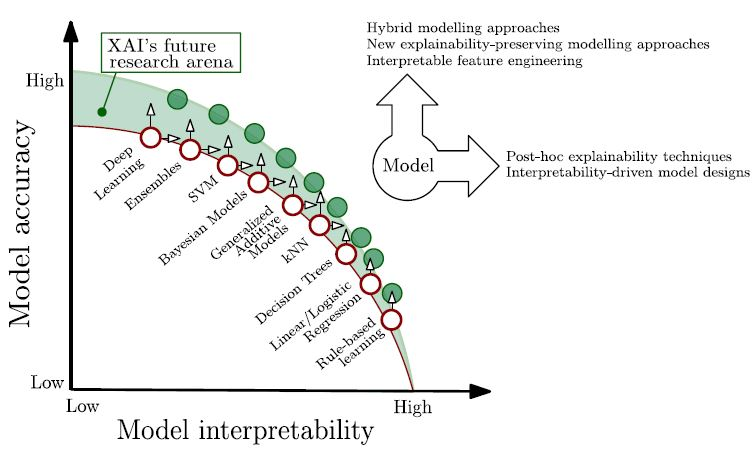
\includegraphics[width=0.8\columnwidth]{figures/XAI_tradeoff.jpg}
  \end{tabular} 
  \caption{Trade-off between model interpretability and model performance \parencite{arrieta2020explainable}.\label{fig:XAItradeoff}}
\end{figure}

Thus, the dichotomy would be between choosing models that provide information about their decisions (known as whitebox models, like a linear regression algorithm), or choosing highly accurate ones that are opaque in that regard (known as blackbox models, like SVM). For many domains, a simple whitebox model may suffice, so both high accuracy and high interpretability are obtained. However, for other more complex domains, high accuracy may only be attainable through blackbox models, thus losing the intepretability information. XAI comes to close the bridge in this dichotomy, providing an additional layer that extracts information about the model's decision. Thus, even if the model is not intepretable by itself, XAI can generate explanations about its decision \parencite{arrieta2020explainable}. 

There are several approaches that can be considered for generating these explanations with XAI. This is something addressed within XAI taxonomies, which classify methods according to different aspects. One of them is related to whether the XAI technique uses specific information that is only available to some blackbox models (model specific), or by contrast, it considers the blackbox model as an "oracle" and infers information about its decision process by analysing its inputs and/or outputs only (model agnositc). An example of the former would be a XAI technique for SVM that uses the information about the support vectors (SV). SV are only available for SVM techniques, and do not exist within other ML algorithms. Thus, the XAI technique only works for a subset of ML algorithms. By contrast, model agnostic techniques could be theoretically be applied to any ML model. This idea is shown in \hyperref[fig:XAIspecificVSagnostic]{Figure} \ref{fig:XAIspecificVSagnostic}.
 
\begin{figure}[h!]
\centering
 \begin{tabular}{c@{\qquad}c@{\qquad}c}
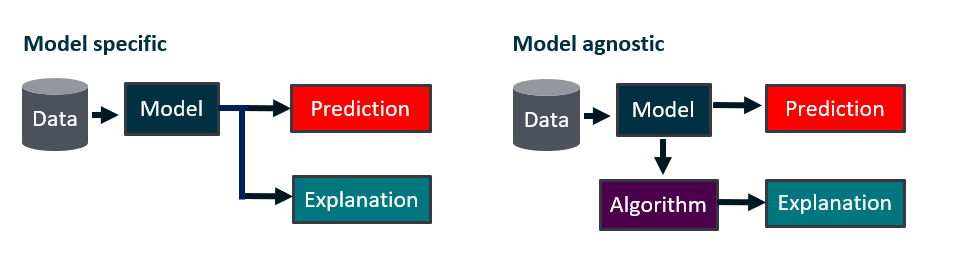
\includegraphics[width=0.8\columnwidth]{figures/XAI_specific_vs_agnostic.PNG}
  \end{tabular} 
  \caption{XAI taxonomy: classifying methods depending on whether they are model specific or model agnostic.\label{fig:XAIspecificVSagnostic}}
\end{figure}

There are other aspects that can be considered for classifying XAI techniques. One of them is the output of the techniques. The XAI technique could be explaining only a specific model prediction (local explanations) or could be explaining the whole decision frontier of the model (global explanations). Also, the explanations could be provided in terms of feature relevance, or could be provided as rule-based explanations \parencite{arrieta2020explainable}. An example of these aspects is shown in \hyperref[fig:XAIapproaches]{Figure} \ref{fig:XAIapproaches}.

\begin{figure}[h!]
\centering
 \begin{tabular}{c@{\qquad}c@{\qquad}c}
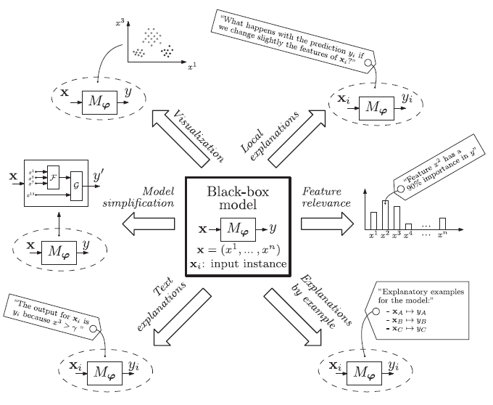
\includegraphics[width=0.6\columnwidth]{figures/XAI_Approaches.PNG}
  \end{tabular} 
  \caption{XAI taxonomy: classifying methods according to their output. \parencite{arrieta2020explainable}\label{fig:XAIapproaches}}
\end{figure}

Finally, beyond the aforementioned taxonomies, there are other important aspects to consider within XAI. Formally, XAI can be defined as "\textit{given an audience, an explainable Artificial Intelligence is one that produces details or reasons to make its functioning clear or easy to understand}" \parencite{arrieta2020explainable}. Thus, XAI must consider not only the underlying model's information, but also the target audience that will receive the explanations. Because of that, XAI is not the same as model intepretability, since the former deals with an active characteristic, while the latter talks about a passive property available to whitebox models only. There are different audiences that can be considered, as shown in \hyperref[fig:XAIaudience]{Figure} \ref{fig:XAIaudience}.

\begin{figure}[h!]
\centering
 \begin{tabular}{c@{\qquad}c@{\qquad}c}
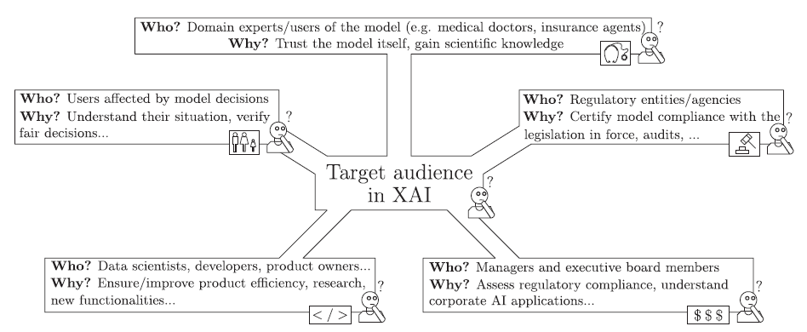
\includegraphics[width=0.8\columnwidth]{figures/XAI_audience.png}
  \end{tabular} 
  \caption{Different types of XAI audiences. \parencite{arrieta2020explainable}\label{fig:XAIaudience}}
\end{figure}


\subsection{Rule extraction techniques in XAI}\label{subsec:ch2-sota-xai-rule-extraction}
As mentioned in the previous subsection, rule extraction methods are a type of post-hoc XAI techniques that have in common that they provide rule-based explanations  \parencite{arrieta2020explainable}. This is exemplified in \hyperref[fig:RuleExtractionExamples]{Figure} \ref{fig:RuleExtractionExamples}, where we see different outputs for rule extraction methods with the case of Decision Trees or rule-based approaches with IF-ELSE rules.

\begin{figure}[h!]
\centering
 \begin{tabular}{c@{\qquad}c@{\qquad}c}
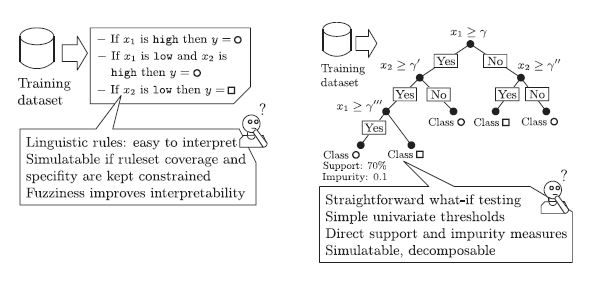
\includegraphics[width=0.8\columnwidth]{figures/RuleExtractionExamples.JPG}
  \end{tabular} 
  \caption{Different examples of rule extraction approaches: through Decision Trees or IF-ELSE rules \parencite{arrieta2020explainable}.\label{fig:RuleExtractionExamples}}
\end{figure}

Beyond that, rule extraction techniques could be classified within any other XAI taxonomy aspect: they can be model agnostic or model specific, or they can provide local and/or global explanations. Within this subsection, we focus on describing different rule extraction techniques depending on whether they are model specific or model agnostic, indicating when these techniques can be used for either global or local explanations (or both).

\subsubsection{Model specific rule extraction techniques in XAI for SVM}\label{subsubsec:ch2-sota-xai-rule-extraction-specific}
\leavevmode\newline
\parencite{barakat2010rule} offers a review of rule extraction techniques for SVM. Focusing on model specific techniques, they highlight three different types of algorithms. The first of them are rule extraction algorithms that use the support vectors from the original model as an input source for generating the rules. This is the case of SQRex-SVM \parencite{barakat2007rule} where the authors propose the usage of a subset of the support vectors for inferring the rules with the usage of a modified sequential covering algorithm. 
The second type of algorithms use both information from the support vectors together with information from the separating hyper-plane. This is the case of RulExSVM \parencite{fu2004extracting}, where the authors propose a technique applicable for SVM with a Radial Basis Function (RBF) kernel. The algorithm uses the support vectors in order to build hyper-rectangles that intersect with the separating hyper-plane. Finally, the last type of techniques use the support vectors, the separating hyper-plane, and the training data. The training data is used to define the regions in the hyperspace, and the support vectors and the hyper-plane define the size of those regions. Within this category appears the proposal of \parencite{nunez2002rule}, which can provide explanations for the whole decision frontier (global), as well as for specific data points (local). We will focus on this last approach since it is the most complete one due to the fact that it uses all the available information for generating the explanations. Their proposal also offers one of the greatest levels of accuracy and fidelity when evaluated over several data sets compared to other proposals.

In \parencite{nunez2002rule}, authors propose a technique called SVM+ Prototypes that can be considered model-agnostic or model specific depending on how is implemented. The general intuition consists in finding hypercubes (or hyperspheres) using the centroids (or prototypes) of data points of each class. Then, it can use as vertices either the support vectors from the SVM model, or the data points from that hyperspace area farther away from that centroid. For the first alternative, the proposal is model specific, since it focuses on a specific component of the model itself (the support vectors). The second one is model-agnostic, since it does not use any information that is specific only for SVM models.
After this, it infers a rule from the values of the vertices of the hypercube that contain the limits of all the points inside it, creating one rule for each hypercube.

For example, a data set that contains two numerical features X and Y will be defined in a 2-dimensional space. The algorithm will create a square that contains the data points on each of the classes, as shown in \hyperref[fig:ch2-sota-outlier0]{Figure} \ref{fig:ch2-sota-outlier0}. The rule that justifies that a data point belongs to class 2 is:
\begin{itemize}
%    \setlength{\itemindent}{2em}
    \item Rule 1: CLASS 2 IF X$\geq$X1 $\land$ Y$\geq$Y1 $\land$ X$\leq$X2 $\land$ Y$\leq$Y2
\end{itemize}

\begin{figure}[h!]
\centering
 \begin{tabular}{c@{\qquad}c@{\qquad}c}
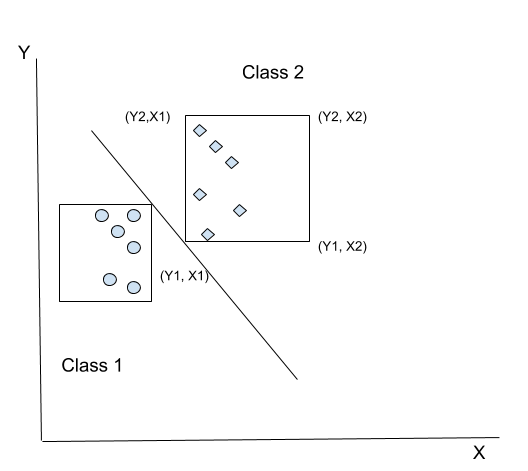
\includegraphics[width=0.5\columnwidth]{figures/outlier_00.png}
  \end{tabular} 
  \caption{SVM with linear kernel classifying data points of two classes.\label{fig:ch2-sota-outlier0}}
\end{figure}

The generated hypercubes may wrongly include points from the other class when the decision frontier is not linear or spherical, as shown in \hyperref[fig:ch2-sota-outlier1]{Figure} \ref{fig:ch2-sota-outlier1}. In this case, the algorithm considers an additional number of clusters trying to include the points into a smaller hypercube, as shown in \hyperref[fig:ch2-sota-outlier2]{Figure} \ref{fig:ch2-sota-outlier2}.

\begin{figure}[h!]
\centering
  \begin{tabular}{c@{\qquad}c@{\qquad}c}
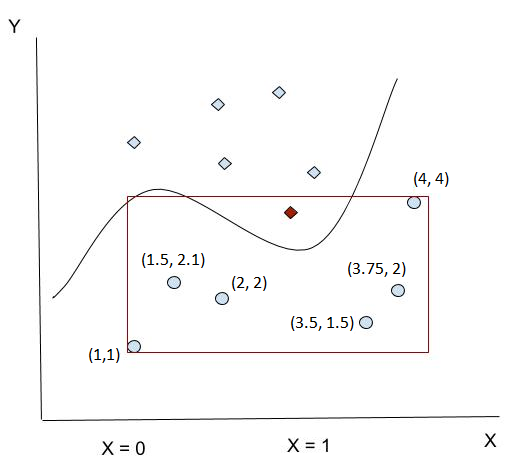
\includegraphics[width=0.5\columnwidth]{figures/outlier_01.png}
  \end{tabular} 
  \caption{A hypercube generated using the farthest points leads to the wrong inclusion of data from the another class.\label{fig:ch2-sota-outlier1}}
\end{figure}

\begin{figure}[!h]
\centering
  \begin{tabular}{c@{\qquad}c@{\qquad}c}
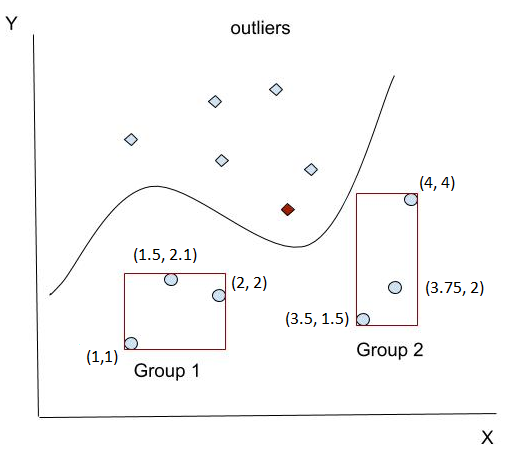
\includegraphics[width=0.5\columnwidth]{figures/outlier_02.png}
  \end{tabular} 
  \caption{Using more hypercubes avoids the aforementioned problem. Now there is no wrong inclusion of data points from another class.\label{fig:ch2-sota-outlier2}}
\end{figure}

A rule will be generated for each hypercube, considering all those scenarios as independent, leading to this output:
\begin{itemize}
    \setlength{\itemindent}{2em}
    \item Group 1: CLASS 1 IF X $\geq$ 1 $\land$ X $\leq$ 2 $\land$ Y $\geq$ 1 $\land$ Y $\leq$ 2.1\
    \item Group 2: CLASS 1 IF X $\geq$ 3.5 $\land$ X $\leq$ 4 $\land$ Y $\geq$ 1.5 $\land$ Y $\leq$ 4
\end{itemize}

There are some downsides of that method in supervised tasks, especially when the problem is not simply a binary classification or when the algorithm is performing a regression. For instance, the number of rules may grow immensely due to the fact that a set of rules will be generated for each category and each set may contain a huge number of rule groups, leading to an output that may be difficult to understand by humans.

However, in OCSVM these difficulties may be potentially mitigated due to two reasons. On the one hand, the explanations are reduced to rules that explain when a data point is not an anomaly (so there would be no need to define rules for the anomalies). On the other hand, the algorithm tries to group all non-anomalous points together, setting them apart from the outliers. Because of this, the chance to define a hypercube that does not contain a point from the another class may be higher than in a standard classification task. Both the unbalanced inherent nature of data points in anomaly detection (few anomalies vs. many more non-anomalous data points) and the fact that non-anomalous points tend to be closer to each other may help achieving good results with this method.

\subsubsection{Model-agnostic rule extraction techniques in XAI}\label{subsubsec:ch2-sota-xai-rule-extraction-agnostic}
\leavevmode\newline
% Some examples
Many rule extraction proposals contribute to XAI without the need to use any specific information from a particular type of model \parencite{arrieta2020explainable}. The only information necessary for building the rules is the input features and the model outputs. Some techniques use all the training data, while others need only a few input instances, or they can even generate artificial data points to infer the decision frontier. An example of this last approach is the LIME (Local Interpretable Model-agnostic Explanations) algorithm \parencite{ribeiro2016should}, where random samples are generated in order to train a linear model that approximates a complex decision function around a specific data point. Following the taxonomy of \parencite{arrieta2020explainable}, model-agnostic techniques through rule-based approaches can be used both for global and for local explanations, as shown in \hyperref[fig:ModelAgnosticDiagram]{Figure} \ref{fig:ModelAgnosticDiagram}.

\begin{figure}[h!]
\centering
 \begin{tabular}{c@{\qquad}c@{\qquad}c}
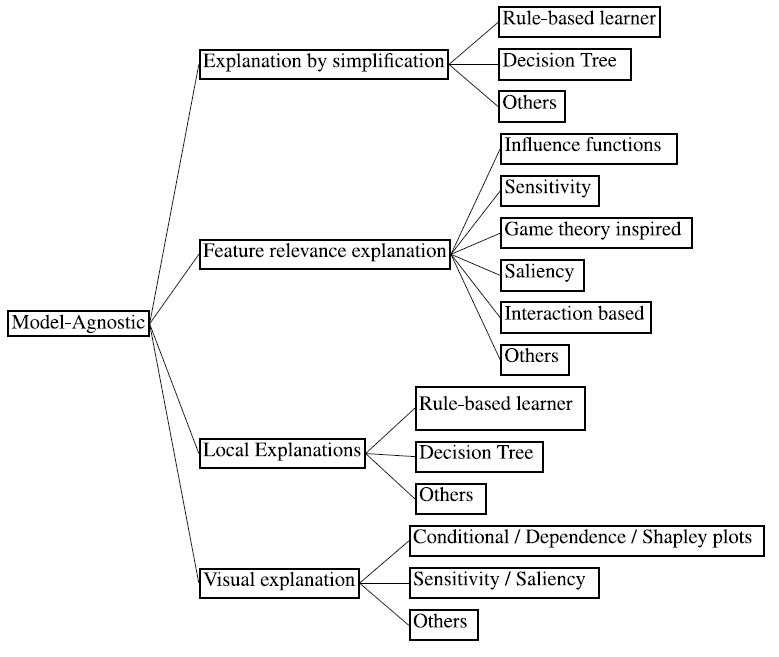
\includegraphics[width=0.7\columnwidth]{figures/ModelAgnosticDiagram.PNG}
  \end{tabular} 
  \caption{Taxonomy for model agnostic XAI techniques, where rule-based approaches appear both for local and global explanations within the case of Decision Trees and Rule-based learners. \parencite{arrieta2020explainable}.\label{fig:ModelAgnosticDiagram}}
\end{figure}

These techniques were initially conceived for supervised ML. However, they can be extended for unsupervised ML for anomaly detection, since their output is analogous to a binary classifier where the classes are heavily imbalanced.

% Surrogate DT
A general way to approximate any blackbox model globally is by using a surrogate supervised decision model trained over the same data set, but instead of using the real labels (the ones used for the blackbox model), it is trained over the predictions of that blackbox model \parencite{molnar2019interpretable}. This may be accomplished with any ML model, but it is useful to do it with a whitebox model that can be directly interpreted by humans. An example is a Decision Tree (DT) model, as indicated in \hyperref[fig:ModelAgnosticDiagram]{Figure} \ref{fig:ModelAgnosticDiagram}. DT allows explaining the classification logic of the blackbox model through the usage of rules, which can be used even for classifying new instances. The advantages of using a DT as a surrogate global model is its flexibility (it can be applied over any model in an agnostic way) and simplicity (it is a solution that is easy to explain). However, this approximation at the end leads to explain a proxy model, and not the actual data, since the surrogate model never sees the true target values.

\hyperref[fig:ModelAgnosticDiagram]{Figure} \ref{fig:ModelAgnosticDiagram} also shows a category of rule-based techniques known as rule-based learners. In many cases, these techniques can be used for both global and local explanations. Following this, we will describe five methods within this category: RuleFit, SkopeRules, Falling Rule Lists, Boolean Decision Rules via Column Generation, and Generalized Linear Rule Models.

% RuleFit
RuleFit \parencite{friedman2008predictive} is a model-agnostic surrogate model that learns a linear regression model (Lasso regression) that uses as features both the original features of the model, as well as new generated features that represent decision rules. In order to accomplish that, first, a tree model is trained over the output and the input features, and the decision paths between the tree levels are turned into decision rules, except for the ones that lead to the leaf nodes, which are not considered. These rules are used as additional features, along with the original ones, on the Lasso surrogate model. Thanks to this, RuleFit yields both rules as well as their contribution, measured through the coefficients of the Lasso model. In summary, RuleFit generates a white-box model that includes rules as features, that can be interpreted as a standard linear regression one. The only caveat is that, for the original coefficients, the predicted outcome changes by $|\beta_j$ if feature $x_j$ changes by one unit if the other features remain unchanged, while for a feature-rule $r_k$ it is different; if all the conditions of the feature $r_k$ are met, the predicted outcome changes by $\alpha_k$ (the weight associated to that rule-coefficient) for regression. Similarly, for classification tasks, when the conditions of $r_k$ are met, the odds for event vs. no-event changes by a factor of $\alpha_k$.

% SkopeRules
Similarly to RuleFit, SkopeRules \parencite{molnar2019interpretable} is another way to generate rules from tree ensembling techniques. They differ, however, in how they obtain the rules. 
First, SkopeRules generates the rules using surrogate tree ensembles trained using the input features and the target variable. Then, it applies a filtering step in which, using a threshold for Precision and Recall, some rules are removed and some are kept. This step allows selecting only high-performing rules, and removing the ones that do not yield good results. The last step is known as "semantic rule duplication". This step eliminates duplicate rules (rules that are the same or very similar to other ones). It also eliminates again low-performing rules based on their results for a F1-metric. This allows obtaining high-performing as well as heterogeneous rules. The final set of rules is the output of SkopeRules, differing from RuleFit because it does not use a Lasso model to aggregate all rules.

% Bayesian Falling Rule List
Falling Rule Lists (FRL) \parencite{wang2015falling} are classification models that generate a sorted list of IF-THEN rules, thus, they can serve as a model-agnostic global post-hoc rule extraction technique. The rules are binary, and are looked one after the other, in order to see if a particular data point can be classified into one of the classes. The rules are sorted according to the probability of classifying a data point into that class using that rule. Due to that, FRL offers a list of IF-ELSE IF rules associated to a particular class with a decreasing probability score. 

% BooleanRuleCG
Boolean Decision Rules via Column Generation (BRCG) \parencite{NIPS2018_7716} also provides a binary classifier by using disjuntive normal form (DNF, OR-of-ANDs) or conjuntive normal form (CNF, AND-of-ORs) through interpretable rules. In case of DNF, they provide an unordered set of decision rules that classify a data point into the positive category if at least one of the rules is satisfied. This is different than other methods already mentioned, such as BFRL where the rules are ordered in an IF-THEN schema, or the surrogate DT model, that provides the rules in a tree structure schema.

% Generalized Linear Rule Models
Generalized Linear Rule Models (GLRM) \parencite{pmlr-v97-wei19a} generate decision rules and combine within a linear model (generalized additive model, GAM). Thus, they provide both a non-linear modelling, thanks to the decision rules, while keeping the interpretability by using a linear model that ensembles them. However, as \parencite{arya2019one} notice, while it is feasible to interpret linear combinations of rules, if the number of rules increases too much, there is a risk of losing the interpretability of the model. The authors highlight that in order to reduce the rules generated and not lose interpretability, they use a rule selection technique based on column generation (CG). CG searches the spaces of rules and generates them only when they are needed, and then fits again the GLM model. This allows analysing again old rules, re-weight them, and discard the ones that are not needed anymore. This is different to other methods used in the literature, mainly pre-selecting a subset of candidate rules using optimization techniques, or a greedy optimization approach by adding rules one by one using sequential covering or boosting techniques.

% Anchors
Within \hyperref[fig:ModelAgnosticDiagram]{Figure} \ref{fig:ModelAgnosticDiagram} there are also other rule-based learner techniques that can only provide local explanations, like Anchors \parencite{ribeiro2018anchors}. The purpose of Anchors is finding a decision rule that approximates the decision function of the blackbox model around that individual data point. This rule "anchors" the prediction of that data point, so that any perturbation of the features of that point that are still inside the rule will always return the same output from the blackbox model. The approach is as follows. First, the algorithm generates candidate rules that may explain the data point. Then, it evaluates those candidate rules. In order to do that, Anchors generates permutations around the data point (similar data points to the original one) that yield the same result. The result is evaluated by calling the blackbox model (the oracle) and obtaining the classification for that data point. In order to optimize the exploration-exploitation of generating and evaluating data points, it uses a reinforcement learning approach with a Multi-Armed Bandit (MAB) approximation. In this MAB, each arm of the Bandit problem is a candidate rule, and the data points generated, after obtaining their classification result from the blackbox model, are used to compute a precision metric used to evaluate the candidate rule's payoff. This reinforcement learning approach helps minimizing the number of calls to the model in order to reduce the computational cost of the algorithm. Among all the candidate rules, the algorithm then checks if the best one of them matches a predefined convergence criteria. To do that, it filters rules according to a precision threshold, and selects form the remaining ones the one with highest coverage. That rule is used to explain that original data point. If there are no rules that match the convergence criteria, then the algorithm keeps iterating (using a beam search approach) using the B best rules from the previous step in order to generate new candidate rules for the following one. In those following steps, Anchors keep extending the rules with more features (in the first step, it only uses one feature per candidate rule).
Thus, Anchors offers a model-agnostic approach that generate IF-THEN rules, easy to interpret, that are generated in an efficient way thanks to the usage of reinforcement learning (MAB) that can be parallelised. However, Anchors is very sensitive to its initial configuration, like many permutation approach algorithms, such as LIME \parencite{ribeiro2016should}. Another important consideration of Anchors is that, while it keeps the calls to the oracle to a minimum (thanks to MAB), it still requires a lot of calls, and that can affect the runtime of the algorithm.

\subsection{Interpretable Machine Learning models}\label{subsec:ch2-sota-interpretable-ml}
Feature relevance-based explanations techniques \parencite{molnar2019interpretable, arrieta2020explainable} quantify the individual contribution of each training feature to the target variable. This type of explanations can be provided either by post-hoc XAI techniques applied to any type of regression or classification ML model, or by using an interpretable ML model alternative. In \parencite{arrieta2020explainable}, the authors propose a guideline for ensuring interpretability in AI models, indicating that a white box algorithmic model should be tried before considering a black box plus an XAI combination. The literature is advancing on the research of white box models that have performances on pair with complex black box ones, to contribute to the usage of models that do not need post-hoc XAI techniques to understand how they took a decision. This is the case of Generalized Additive Models (GAM) \parencite{hastie1987generalized}. In GAM models, the input features and the output have an additive relationship, with each term contributing independently. Therefore, they can be used for knowing the individual impact of each feature in the output for a particular feature value. This idea is similar to Linear Regression models, but the main difference is that the individual relationship between a feature and the output is not constant; is a function that may even be nonlinear. GAM is improved by $GA^2M$ algorithm \parencite{lou2013accurate}, implemented in Explainable Boosting Machine (EBM) algorithm \parencite{nori2019interpretml}. An additional evolution over the previous algorithm is Constrained Generalized Additive 2 Model with Consideration of Higher-Order Interactions (CGA2M+) \parencite{watanabe2021cga2mplus}. CGA2M+ includes two improvements over EBM. First, it allows to specify monotonic constraints, so the functions that model the relationship between an input feature and the output may be monotonic. Second, the model allows using higher-order interactions, as opposed to EBM, where the interactions are limited to second-order. \hyperref[eq:ch2-sota-GAM]{Equation} \ref{eq:ch2-sota-GAM} shows the original GAM structure, with $\beta_0$ the intercept, $i$ a particular feature, $x_i$ its corresponding feature value, $f_i$ the function that models the relationship with the output and $g$ the link function. \hyperref[eq:ch2-sota-EBM-pairwise]{Equation} \ref{eq:ch2-sota-EBM-pairwise} shows the $GA^2M$ algorithm, including the pairwise terms through $\sum f_{ij}(x_{i}, x_{j})$, which models the joint contribution of feature $i$ with feature $j$ through an additional function $f_{ij}$.
\hyperref[eq:ch2-sota-GA2M+]{Equation} \ref{eq:ch2-sota-GA2M+} shows the CGA2M+ algorithm, allowing to include higher-order terms that model the relationship between more than two features $x_i, ..., x_k$.

\begin{equation}\label{eq:ch2-sota-GAM}
g(E[y]) = \beta_0 + \sum_{n=1} f_{i}(x_{i})
\end{equation}

\begin{equation}\label{eq:ch2-sota-EBM-pairwise}
g(E[y]) = \beta_0 + \sum f_{i}(x_{i}) + \sum f_{ij}(x_{i}, x_{j})
\end{equation}

\begin{equation}\label{eq:ch2-sota-GA2M+}
g(E[y]) = \beta_0 + \sum f_{i}(x_{i}) + \sum f_{ij}(x_{i}, x_{j}) + f_{high}(x_{i},..., x_{k})
\end{equation}

\section{Metrics for XAI}\label{sec:ch2-metrics-xai}
In this section, we approach another important aspect within XAI: the field of XAI metrics, which aims to provide quantitative evaluations to assess the quality of the explanations generated. The review of \parencite{arrieta2020explainable} identifies the necessity of metrics to assess the understandability of the explanations generated. The authors propose the following definition of explainability: \textit{"Explainability is defined as the ability a model has to make its functioning clearer to an audience}". There are several taxonomies of XAI metrics proposed in the literature to address that. 

In \parencite{carvalho2019machine}, the authors analyse the literature and define a taxonomy of properties that should be considered in the individual explanations generated by XAI techniques. Even though the paper deals with quantifying the quality of the explanations for an individual data point, some of them are also applicable for global explanations.
\begin{itemize}
    \item \textbf{Accuracy}: It is related to the usage of the explanations to predict the output using unseen data by the model. 
    \item \textbf{Fidelity}: It refers to how well the explanations approximate the underlying model. The explanations will have high fidelity if their predictions are constantly similar to the ones obtained by the blackbox model. Accuracy and fidelity are intertwined: If the explanations have high fidelity (thus, approximate the model well) and the model has high accuracy, the explanations will also have high accuracy. However, the explanations may have high accuracy (because they predict very well over unseen data) while having low fidelity (because they do not approximate well the original model)
    \item \textbf{Consistency}: It refers to the similarity of the explanations obtained over two different models trained over the same input data set. High consistency appears when the explanations obtained from the two models are similar. However, a low consistency may not be a bad result since the models may be extracting different valid patterns from the same data set due to the "Rashomon Effect" (seemingly contradictory information is fact telling the same from different perspectives).
    \item \textbf{Stability}: It measures how similar the explanations obtained are for similar data points. Opposed to consistency, stability measures the similarity of explanations using the same underlying model.
    \item \textbf{Comprehensibility}: This metric is related to how well a human will understand the explanation. Due to this, it is a very difficult metric to define mathematically, since it is affected by many subjective elements related to human's perception (such as context, background, prior knowledge, etc.). However, there are some objective elements that can be considered in order to measure "comprehensibility", such as whether the explanations are based on the original features (or based on synthetic ones generated after them), the length of the explanations (how many features they include), or the number of explanations generated (i.e. in the case of global explanations). In general terms, using the original features, while keeping the number of explanations generated and the features used to a minimum, will increase comprehensibility.
    \item \textbf{Certainty}: It refers to whether the explanations include the certainty of the model about the prediction or not (i.e. a metric score).
    \item \textbf{Importance}: Some XAI methods that use features for their explanations include a weight associated with the relative importance of each of those features. 
    \item \textbf{Novelty}: Some explanations may include whether the data point to be explained comes from a region of the feature space that is far away from the distribution of the training data. This is something important to consider in many cases, since the explanation may not be reliable due to the fact that the data point to be explained is very different from the ones used to generate the explanations.
    \item \textbf{Representativeness}: It measures how many instances are covered by the explanation. Explanations can go from explaining a whole model (i.e. weights in linear regression) to only be able to explain one data point. 
\end{itemize}

Considering the case of rule extraction techniques, the outputs (rules) for the whole data set can be analyzed from the perspective of global explanations. In this context, one additional aspect to consider is \textbf{diversity}, a metric that indicates whether the explanations are redundant or repetitive and can already be mostly covered by another explanation, or if they provide insights that are not deducible from the other explanations available. 

\parencite{hoffman2018metrics} proposes another taxonomy, which includes metrics for \textit{precision} together with metrics that measure how helpful the explanations are to the users that receive them (with metrics like \textit{explanation satisfaction}, \textit{understandability}, \textit{completeness}, \textit{usefulness} or \textit{feeling of satisfaction}). 

These metric taxonomies are being used to build quantitative metrics for the explanations, as shown in \parencite{melis2018towards}. They first consider three families of metrics, \textit{explicitness}, \textit{faithfulness} and \textit{stability}. Then, they propose several algorithms to infer them, evaluating the results over different data sets. The \textit{stability}
metric computes the norm of the difference for the explanation-based predictions for the two closest data points within the data set. These two data points are found by using a K-Nearest Neighbours algorithm over the same input features used for training the ML surrogate model. This value is then scaled considering the distance between those two data points (in order to penalize the metric if they are not very close). The formula appears in \hyperref[eq:ch6-stability-metric-sample]{Equation} \ref{eq:ch6-stability-metric-sample}, where $x_i$ and $x_j$ are two data points, $f_{expl}$ the predictions based explanations for those data points, and $h$ the distance between them.

\begin{equation}\label{eq:ch6-stability-metric-sample}
\qquad 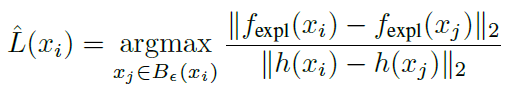
\includegraphics[width=200pt]{figures/stability_metric.PNG}
\end{equation} 

\parencite{barakat2010rule} already commented on the importance of comprehensibility, accuracy and fidelity for rule extraction techniques that explain a SVM model though rule extraction techniques. The metrics are defined as:
\begin{itemize}
    \item \textbf{Accuracy} = Number of instances classified correctly by the rules / Length test set
    \item \textbf{Fidelity} = Number of instances where the rule predictions match the model predictions / Length test
    \item \textbf{Consistency} = Number of of rules and No. of antecedents (analogous to rule size).
\end{itemize}

\parencite{vilone2020comparative} shows a model-agnostic comparative for rule extraction algorithms using C4.5Rule-PANE, REFNE, RxREN and TREPAN. For that, they use 8 data sets of up to 8124 total instances and 40 features. As blackbox models they use Neural Networks models for classification (with different configurations). Finally, they propose several metrics for measuring the quality of the explanations.

\begin{itemize}
    \item \textbf{Completeness:} Percentage of input instances covered by rules over total input instances. Analogous to "Representativeness".
    \item \textbf{Correctness:} Percentage of input instances correctly classified by rules over total input instances. Analogous to "Accuracy".
    \item \textbf{Fidelity:} Percentage of input instances on which the predictions of model and rules agree over total instances.
    \item \textbf{Robustness:} Applying small perturbations over the data points that do not change the prediction of the model, the sum of differences between the original prediction and the new prediction, divided by the number of instances analyzed. It is analogous to the concept of "Stability".
    
    \begin{equation}
    \begin{split}
      Robustness = \frac{\sum_{n=1}^{N} f(x_n) - f(x_n + \delta)}{N} \\
    \end{split}
    \end{equation}
    
    Robustness is further analysed in \parencite{alvarez2018robustness}, where the authors evaluate it for feature relevance model-agnostic post-hoc XAI techniques (LIME and SHAP).
        
    \item \textbf{Number of rules} and \textbf{Average rule length}, similar to \parencite{barakat2010rule}.
\end{itemize}

They apply these metrics and see, using the Friedman's test, that C45-Pane has significantly superior results over all of the data sets considering all of the metrics, followed by TREPAN.

A summary of all these proposal appears in \hyperref[table:ch2-sota-taxonomy-sota]{Table} \ref{table:ch2-sota-taxonomy-sota}, including some direct mappings between them. 

\begin{table}[h!]
\centering
\resizebox{220pt}{!}{%
\begin{tabular}{@{}llllll@{}}
                                                     & \rot{{\parencite{carvalho2019machine}}}
                                                     & \rot{{\parencite{hoffman2018metrics}}}
                                                     & \rot{{\parencite{melis2018towards}}}
                                                     & \rot{{\parencite{barakat2010rule}}} 
                                                     & \rot{{\parencite{vilone2020comparative}}}
                                                     \\ \midrule
\multicolumn{1}{l|}{Accuracy/Correctness}            & X & X &   & X & X \\
\multicolumn{1}{l|}{Fidelity/Faithfulness}           & X &   & X & X & X \\
\multicolumn{1}{l|}{Consistency}                     & X &   &   &   & X \\
\multicolumn{1}{l|}{Stability/Robustness}            & X &   & X & X &   \\
\multicolumn{1}{l|}{Comprehensibility}               & X & X &   & X &   \\
\multicolumn{1}{l|}{Certainty}                       & X &   &   &   &   \\
\multicolumn{1}{l|}{Importance}                      & X &   &   &   &   \\
\multicolumn{1}{l|}{Novelty}                         & X &   &   &   &   \\
\multicolumn{1}{l|}{Representativeness/Completeness} & X &   &   & X &   \\
\multicolumn{1}{l|}{Contrastiveness}                 & X &   &   &   &   \\
\multicolumn{1}{l|}{Selectivity}                     & X &   &   &   &   \\
\multicolumn{1}{l|}{Social}                          & X &   &   &   &   \\
\multicolumn{1}{l|}{Focus on the abnormal}           & X &   &   &   &   \\
\multicolumn{1}{l|}{Truthful}                        & X & X &   &   &   \\
\multicolumn{1}{l|}{Consistent with apriori beliefs} & X &   &   &   &   \\
\multicolumn{1}{l|}{General and probable}            & X &   &   &   &   \\
\multicolumn{1}{l|}{Explicitness}                    &   &   & X &   &   \\
\multicolumn{1}{l|}{Feeling of Satisfaction}         &   & X &   &   &   \\
\multicolumn{1}{l|}{Usefulness}                      &   & X &   &   &   \\
\multicolumn{1}{l|}{Completeness}                    &   & X &   &   &   \\
\multicolumn{1}{l|}{Sufficiency of Detail}           &   & X &   &   &   \\ \bottomrule
\end{tabular}%
}
\caption{Summary of the metric properties for XAI within the referenced literature, including some direct mappings between them.}
\label{table:ch2-sota-taxonomy-sota}
\end{table}


\section{XAI for anomaly detection}\label{sec:ch2-sota-xai-anomaly-detection}
After describing general aspects about XAI, in this section, we focus on the literature regarding XAI and anomaly detection through several aspects. First, we provide an introduction to the specific literature about XAI and anomaly detection, focusing on previous research regarding XAI and OCSVM. Then, we cover another aspect that is relevant for XAI in general, and for XAI for anomaly detection in particular: XAI with prior domain knowledge. 

\subsection{Introduction}\label{subsec:ch2-sota-xai-anomaly-detection-intro}
XAI is useful for both explaining an anomaly detection model from a global perspective, or for explaining the identification of particular instances as outliers. From the global explanation level, \parencite{tallon2020explainable} use two anomaly detection ML algorithms (Decision tree and DeepLog) to detect outliers. Together with that, they use Shapely values in order to generate model-agnostic feature relevance explanations that help to see which features contribute more for predicting outliers by seeing the individual contribution of each feature to the general outlier probability. 

XAI has also been used for anomaly detection for predictive maintenance \parencite{langone2020interpretable}. The authors highlight that even when an anomaly detection model is very accurate, the operators that will get the model prediction may not trust it if it remains a blackbox that does not provide any insights about its decisions. Because of that, they propose an anomaly detection system where the explanations are generated thanks to the usage of a whitebox model (ElasticNet Logistic Regression). So, they provide explanations in terms of feature relevance, focusing on explaining what contributes to an anomalous state. With that, they highlight that explanations for anomaly detection can be generated in a similar way to those of a supervised ML model for binary classification (even though anomaly detection models provide an output heavily imbalanced) 

Shapely values for explaining anomalies are also used at \parencite{mitani2020highly}, where the SHAP algorithm is used to generate feature relevance explanations in order to explain what contributes to specimen mix-up. For the anomaly detection, they use a Gradient Boosting Tree in order to be able to learn efficiently from highly unbalanced data while yielding good predictions. The authors highlight the importance of having a highly accurate model that is able to predict correctly the specimen mix-up, because this is a crucial problem that may lead to an incorrect diagnostic or an inappropriate therapy.

An additional recent reference of XAI for anomaly detection is \parencite{ruff2021unifying}. Their focus on explanations is mainly for unsupervised deep learning (DL) models, where the explanations can be produced by model-agnostic post-hoc techniques for feature relevance (LIME) or by using model specific algorithms (LRP). One of the usages of XAI that they describe is the improvement of the model based on the explanations provided. They show an example for anomaly detection based on images, where XAI helps to see the cases where the pixels used for making the decision are actually the correct ones.

The analysis of the literature highlights how detecting anomalies is critical within some domains, and because of that, their detection needs to be very precise. However, being able to detect anomalies is not enough, and explanations are needed for both understanding the model better (and seeing if it can be trusted or improved), as well as for explaining the model for other audiences in order to see if they can also rely on the predictions or not (something connected to the explanation generation for different user profiles \parencite{arrieta2020explainable}). A model may perform apparently very well and explanations may help to see that the model is taking its decision by using features that are not relevant \parencite{molnar2019interpretable}, so in that case, the model may not be finally trusted. This shows that XAI can complement the classical evaluation of models based only on their performance.

However, after the assessment of a model and seeing that it behaves correctly (from both the XAI and the performance point of view), before providing explanations to some user profiles, it is important to ensure that they are aligned to what the model predicts, and are not showing any contradictory information. One way to accomplish that within the scenario of rule extraction techniques is by using P@1 rules with respect to the model output. Here, the rules may not be explaining all the possible model's outputs, but the explanations will never contradict it.

For feature relevance explanations, the literature shows that they help to see how they contribute to the positive class (outliers in anomaly detection). For rule extraction explanations, they can help to explain outliers with respect to what will turn that outlier into an inlier. Considering this, the explanations will target the inlier class, so the outliers can be explained in a counterfactual approach with respect to the non-anomalous subspace (for local explanations). For global explanations that help to see what feature values are normally associated to outlier situations, the explanations would still target the outlier class.


\subsection{XAI for OCSVM}\label{subsec:ch2-sota-xai-oscvm}
Searching in the Scopus\textsuperscript{\textregistered} \footnote{Last searched in 01/02/2020.} database for titles, abstracts, and/or keywords that contain the terms "XAI", "explainable" or "interpretable", together with "OC-SVM" or "OCSVM", only provided 4 results.

One of them is the work of \parencite{kauffmann2020towards}. Here, the authors propose a model-specific method based on the fact that OCSVM models can be rewritten as pooling neural networks. Due to the asymmetry between inliers and outliers, they model with a min-pooling over distances for outliers, and a max-pooling over similarities for inliers. Thanks to turning OCSVM models to a neural network, they apply a deep Taylor decomposition (DTD) to obtain explanations in terms of input features. DTD serves as a framework to apply layer-wise retropropagation (LRP) in order to obtain the feature contribution of the input features to a predicted output. The authors extend the explanations generated to include using both input features or support vectors. 

In \parencite{itani2020one} the authors benchmark different unsupervised ML algorithms for anomaly detection (IsolationForests, OCSVM, Cluster Support Vector Data Description and One-Class decision Tree, OC-Tree), and analyse them over data from the medical domain. They indicate that OC-Tree provides the best results, with the advantage of being a hybrid method that combines the first kernel density estimation for anomaly detection with a decision tree that automatically provides rules that explains the first model. The benchmark of the models is performed in terms of predictive performance, mentioning that OC-Tree is then better for that use case since it directly provides explanations.

In \parencite{jang2019anomaly} the authors use OCSVM and Variational Autoencoders for detecting engine faults within 2.4L diesel engines. The faults, which may belong to two types, are precisely the anomalies. For that they use 130 feature parameters. Together with that, they include a post-hoc explainability layer by using LIME (thus, explaining the models in terms of feature relevance).

\parencite{padmaja2015hybrid} also shows the combination of OCSVM with XAI. For the XAI part, they use the algorithm Ripper for rule induction. For this algorithm, they use the information from the support vectors from the OCSVM. At the evaluations, they use three different data sets and measure the performance of the rules extracted in terms of Precision, Recall and F1 metrics over the ground truth of the real anomalies. They also train OCSVM models with a RBF kernel.

The previous analysis of the literature shows that even though there are some works regarding XAI and OCSVM, they are either focused in a particular domain, or they do not compare several XAI methods in order to assess their differences (from either a model's performance or explanainability point of view). Due to that, there is still an open area regarding the benchmark of rule extraction techniques over OCSVM models for anomaly detection.

\subsection{Domain knowledge combined with XAI}\label{subsec:ch2-domain-knowledge-xai}
Within the review of \parencite{arrieta2020explainable}, one of the open research challenges is combining domain knowledge with the explanations generated to enhance the user's understandability. This challenge is especially addressed through the combination of deep learning black box models together with symbolic approaches (as covered within the field of neurosymbolic approaches). These last approaches are algorithmic transparent and generally directly interpretable, and with domain knowledge expressed through ontologies. This is the case of \parencite{confalonieritrepan}, where the authors propose a variant of the TREPAN algorithm that uses domain ontologies in the XAI phase. TREPAN uses surrogate decision trees to explain any black box model (model agnostic). However, as the authors highlight, those trees are often not understandable by a final user. That is why they propose a variation on the algorithm that gathers information from a domain ontology and uses it to prioritize using features for the splits that are more general within the ontology. The prioritization is done by penalizing the Information Gain value when considering a feature from the split that is too specific.  They assessed their proposal with expert users in the finance and medical domains, and found that using domain knowledge enhances the user's understandability.

Indeed, domain knowledge can be applied to adjust the explanations generated, and it can be done at different moments during a ML model life cycle. It can be done at the ML model itself (for instance, finding hyperparameters that enhance the model understandability), or during the training of a post-hoc XAI method. Finally, it can be also applied after the XAI method generates the explanations, to adjust them to the existing domain knowledge. This is shown within the literature review of \parencite{beckh2021explainable}. Authors indicate how there are three scenarios regarding XAI and prior domain knowledge. First, mainly for posthoc approaches, integrating the knowledge at the underlying ML level either by combining it with the data set, during the grid search for adjusting the hyperparameters, for defining the cost function, or for postprocessing the output (e.g., for choosing the classification threshold). Second, by integrating the knowledge within the XAI method (with similar sub-approaches as the ones for the integration with the underlying ML method). Finally, they also indicate cases where new knowledge can be derived from the explanations, such as detecting bias problems with the ML model thanks to XAI, or building new applications and use cases thanks to the XAI explanations.

The combination of domain knowledge and XAI is crucial, since this helps preventing the generation of explanations that only explain the model decision in terms of correlations, ignoring any causality aspects, which can led explanations that are false or misleading \parencite{holzinger2019causability}.

\section{Introduction to anomaly detection in real-world contexts}\label{sec:ch2s-sota-specific}
%Within this section, we review the SOTA regarding the factors that impact on the fuel consumption of diesel and petrol vehicles, since this is one of the main use cases studied within this thesis. This analysis is important for eliciting the features for training the ML models, as well as for analysing if the explanations are aligned to that prior domain knowledge. We also review previous literature regarding vehicle fuel prediction with some of these factors using ML, as well as the usage of anomaly detection models for detecting vehicle fuel anomalies.

In this section, we review the SOTA regarding anomaly detection within real-world contexts, particularly for the use cases of Mobile Network Operators (MNO) covered in this thesis: anomaly detection in network communications data, and anomaly detection in vehicle fuel usage. We will describe the context of anomaly detection within these contexts, along with the techniques used related to ML. We will also highlight the features that are normally used for identifying the anomalies in those contexts. This analysis is important for eliciting the features for training the ML models, as well as for analysing if the explanations are aligned to that prior domain knowledge.

\subsection{Anomaly detection in network traffic}\label{subsec:ch2-sota-comms}

% Reviews of anomaly detection in network traffic
The problem of anomaly detection within network traffic is a common use case within MNO since it is crucial within several applications. The review of \parencite{fernandes2019comprehensive} highlights how important it is to detect anomalies in order to avoid significant service degradation, malicious damage or for reducing costs. An anomaly could be considered as a "\textit{observation (or subset of observations) which appears to be inconsistent with the remainder of that set of data}" \parencite{barnett1984outliers}, though it is important having a prior knowledge about the type of anomalies in order to address the problem properly. For traffic anomalies, they classify the literature depending on the nature of the anomalies (point, collective or contextual), or on the causal aspect (operational, flash crowd, measurement,  or network attack). 
Regarding the nature:
\begin{itemize}
\item \textbf{Point anomaly}: A single data point has a different behaviour compared to its data group
\item \textbf{Contextual anomaly}: Data is anomalous within a specific context. This is common within time series, where an anomaly may happen during a specific time interval (but outside it, that same point would not be anomalous).
\item \textbf{Collective anomaly}: A collection of data groups have an anomalous behaviour within the whole data set.
\end{itemize}

This classification of anomalies based on their nature is not specific to network traffic. Nonetheless, the authors also classify the literature based on the causal aspect, specific to network anomalies:
\begin{itemize}
\item \textbf{Operational events}: Server crashes, power outages, traffic congestion, large transfers (non-malicious), inadequate resource configuration.
\item \textbf{Flash crowds}: Legitimate but abnormal use. Large flows in traffic normally caused by a rapid growth of users trying to access a specific network resource (e.g., an e-commerce website announces a promotion and a lot of people access the site simultaneously)
\item \textbf{Measurement anomalies}: Other type of anomalies different from the ones above, and that are also non-malicious. They are related to problems during the data collection phase.
\item \textbf{Network abuse anomalies}: They are malicious attempts to disrupt, deny, degrade or destroy information and services from computer network systems.
\end{itemize}

They also provide a taxonomy based on the techniques used for anomaly detection, which is also something that can be used within other use cases. They classify the literature depending on whether they use evolutionary computation, finite state machine, clustering, information theory, classification, statistical or other techniques.

The review of \parencite{ali2020review} indicates similar taxonomy approach for network anomaly detection, using the same classification for the nature of the anomalies, and providing classification based on the ML techniques used. For this last aspect, they indicate techniques related to supervised classification (SVM, Naive Bayes, Neural Networks, Nearest Neighbours or Decision Trees), semi-supervised learning, or unsupervised learning (mainly related to different types of clustering techniques).

% Anomaly detection in MNO
The work of \parencite{gunavathi2019big} presents a proposal for anomaly detection within Call Detail Records (CDR) data, using unsupervised clustering techniques. They first define a set of features related to the call-in (received calls) and call-out (outgoing calls) information, and then they generate a feature that indicates the activity for that particular CDR. With that and using the clustering techniques, they group the CDRs based on the behaviour, and they use that for finding CDRs that are anomalous based on their activity. Activity could be anomalous either because it is to high or it is too low compared to the normal behavioural pattern.

% Anomaly detection in Call Centers
For the particular case of Call Centers, the work of \parencite{iheme2019feature} presents the usage of OCSVM models for detecting anomalies within the calls in order to detect potential malpractices in the agents. They use several features are used for modelling the calls: call duration, average silence duration, dBFS (loudness of the call), or the percentage of silence, among others.

% Finally, only reference that combines XAI and anomaly detection within a MNO use case
However, even though the literature is extensive in terms of network anomaly detection (and related use cases), there is a lack of research regarding the usage of XAI in these contexts. The only explicit reference for XAI for anomaly detection for network related use cases is, to the best of our knowledge, the recent work of \parencite{irarrazaval2021telecom}. There, authors research anomaly detection on traffic networks to detect traffic pumping. Traffic pumping is a type of fraud that happens in some countries, where a local operator with high access charge rate has an agreement with another one with high call volume operations (which is usually free of charge), so the number of calls into the local operator is stimulated, then sharing a portion of its increased access revenues with the bigger one. For their use case, there are no labels, so they use unsupervised clustering for finding the anomalies. They use then a decision tree using the clustering labels as prediction labels, and they infer rules about each group. These rules are given to telecommunications experts so they can validate them or study the corresponding cluster in more detail, and identify which groups are anomalous. Thus, they do provide a XAI based solution which through a global surrogate post-hoc model (Decision Tree) that explains with rules the relationship between input features and output clustering labels. They also built a set of features that can be easily incorporated in an explanation (an important aspect in order to enhance the understandability aspect \parencite{arrieta2020explainable}).


\subsection{Factors for fuel consumption in a vehicle}\label{subsec:ch2-sota-fuel-factors}
In the previous subsection we indicated how the detection of anomalies in real-world contexts requires the use of prior domain knowledge, and this step is crucial for choosing the set of features for both detecting and explaining these anomalies. Thus, in this subsection, we will analyse in detail the features that may impact on the fuel usage, since it is a field very well researched.

Fuel consumption can significantly vary from one vehicle to another, even when comparing two vehicles from the same make, model, year and fuel type. This is caused by different factors that may increase or decrease the amount of fuel consumed during the same trip. The literature contains many studies that identify these factors and assess how much fuel could be saved when they are optimized. This is something very relevant for fleet managers.

\parencite{zhou2016review} presents a literature review of different factors that have a potential impact in the fuel consumption of a vehicle, together with their relative importance. \hyperref[figure:ch2-sota-chart-factors]{Figure} \ref{figure:ch2-sota-chart-factors} shows the categories of fuel factors considered in that review. 

\begin{figure}[h!]
\centering
 \begin{tabular}{c@{\qquad}c@{\qquad}c}
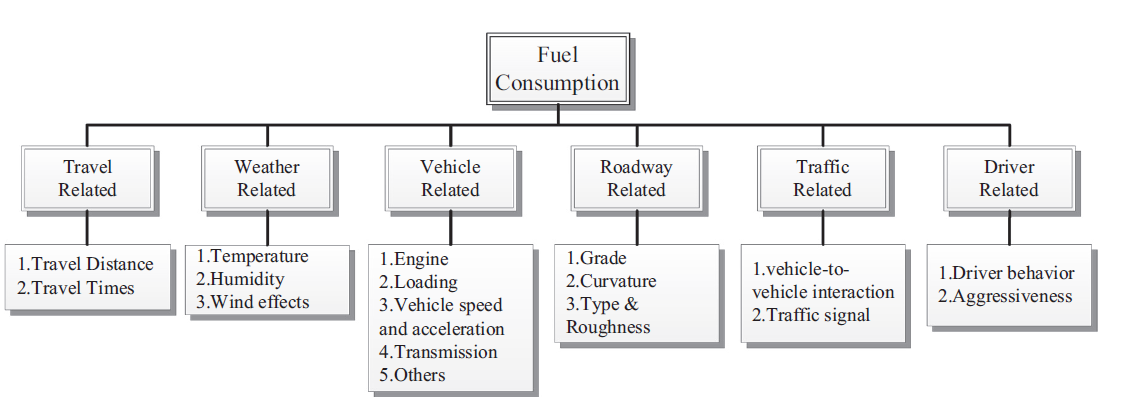
\includegraphics[width=0.8\columnwidth]{figures/chart_factors.PNG}
  \end{tabular} 
  \caption{Categories of fuel factors discussed in \parencite{zhou2016review} \label{figure:ch2-sota-chart-factors}}
\end{figure}

The first category considered are \textbf{travel-related} factors. This group includes factors that are related to the route covered by the vehicle. In fact, the authors mention \textbf{eco-routing} as a crucial aspect to reduce fuel consumption. Fuel can be saved by choosing an optimal route not only in classical terms of distance and travel time, but also in terms of a route that saves fuel compared to other possible ones (e.g.choosing routes with less "bumps" or "slopes"). In fact, the new route may even be longer in time or distance, but offers fuel saving. The paper indicates that eco-routing alone can reduce the fuel consumption of a vehicle by 18\% to 23\%.

The second category includes \textbf{weather-related} factors. These factors impact the fuel consumption of a vehicle in an indirect way (i.e. by being related to the usage of the air conditioner, by affecting the water pump, by increasing the engine or transmission friction in a cold weather...). Thus, this category includes factors like the exterior temperature, the relative humidity or the wind effects. These factors may be responsible for about a 1\% of the fuel consumption of a vehicle.

The third group of factors are named \textbf{vehicle-related}. It includes factors mainly related to the engine and the vehicle itself, such as vehicle load, vehicle speed, engine speed, type of fuel, whether the vehicle has an exhaust after-treatment system or not... 

The fourth group is named \textbf{roadway-related factors}. It refers to factors related to the road condition, like the road slope, the surface roughness, or the road curvature. These factors, though not being very actionable (sometimes it is difficult to prevent them), have a large impact on the fuel consumption (around 5 to 20\%).

The fifth group of factors refer to \textbf{traffic conditions}. They are very related to a good arrangement of traffic signs, such as traffic lights. They have the potentially biggest fuel impact (around 22 to 50\% of the fuel consumption).

Finally, the sixth group mentioned in the review are the \textbf{driver-related} factors, like the driving behaviour or the aggressiveness of the driving. The driving profile of a particular driver (that measures aspects such as that driving aggressiveness), are calculated with vehicle information such as the RPM (engine speed; revolutions per minute), the speed or the acceleration. The authors mention how aggressive driving can be responsible for up to 40\% of the fuel consumption of a vehicle when compared to a calmer driving style. 

The aforementioned literature review is enhanced by the study of \parencite{zacharof2016review}. Here the authors present a thorough analysis regarding the influence of different factors for fuel consumption in a vehicle, along with the influence on CO2 emissions. This study considers passenger vehicles under real-world operating conditions. Regarding fuel consumption specifically, the authors offer a summarized view of the literature showing different categories of variables and their proportional impact in the fuel consumption of a vehicle. 

There are two approaches for analysing the impact of a specific factor in the fuel consumption of a vehicle. First, using a simulation analysis that studies the isolated impact of a factor under laboratory conditions. Second, by analysing feeds of data that contain the instant fuel consumption reported during trips on real-world environments. These feeds of data can be gathered from sources such as OBD-II (On-board diagnostics) port \parencite{ISO14230} (e.g. the Engine Fuel Rate with the PID 015E). 

The analysis of the literature highlights that both approaches offer in general similar results (when there are publications available for a specific factor both from the simulation point of view, as well as with the real-world data). Thus, real-world collected data can be a valid data source for assessing the impact of different factors in the fuel consumption of a vehicle.

Here, the literature review proposes a fuel factor taxonomy that in some cases matches directly the one proposed in \parencite{zhou2016review}, but in some others is different. There are 28 factors that can be classified into 9 groups. All these factors, as reported by \parencite{zacharof2016review}, appear at \hyperref[table:ch2-sota-factors-table]{Table} \ref{table:ch2-sota-factors-table}. This Table shows the relative importance of each of the factors (literature median value) along with an interval that encloses the different values reported, considering vehicles under real-world operating conditions. It also shows how many papers talk about that particular factor, as well as the distribution of the relative values reported. 

\begin{sidewaysfigure}[h!]
  \centering
  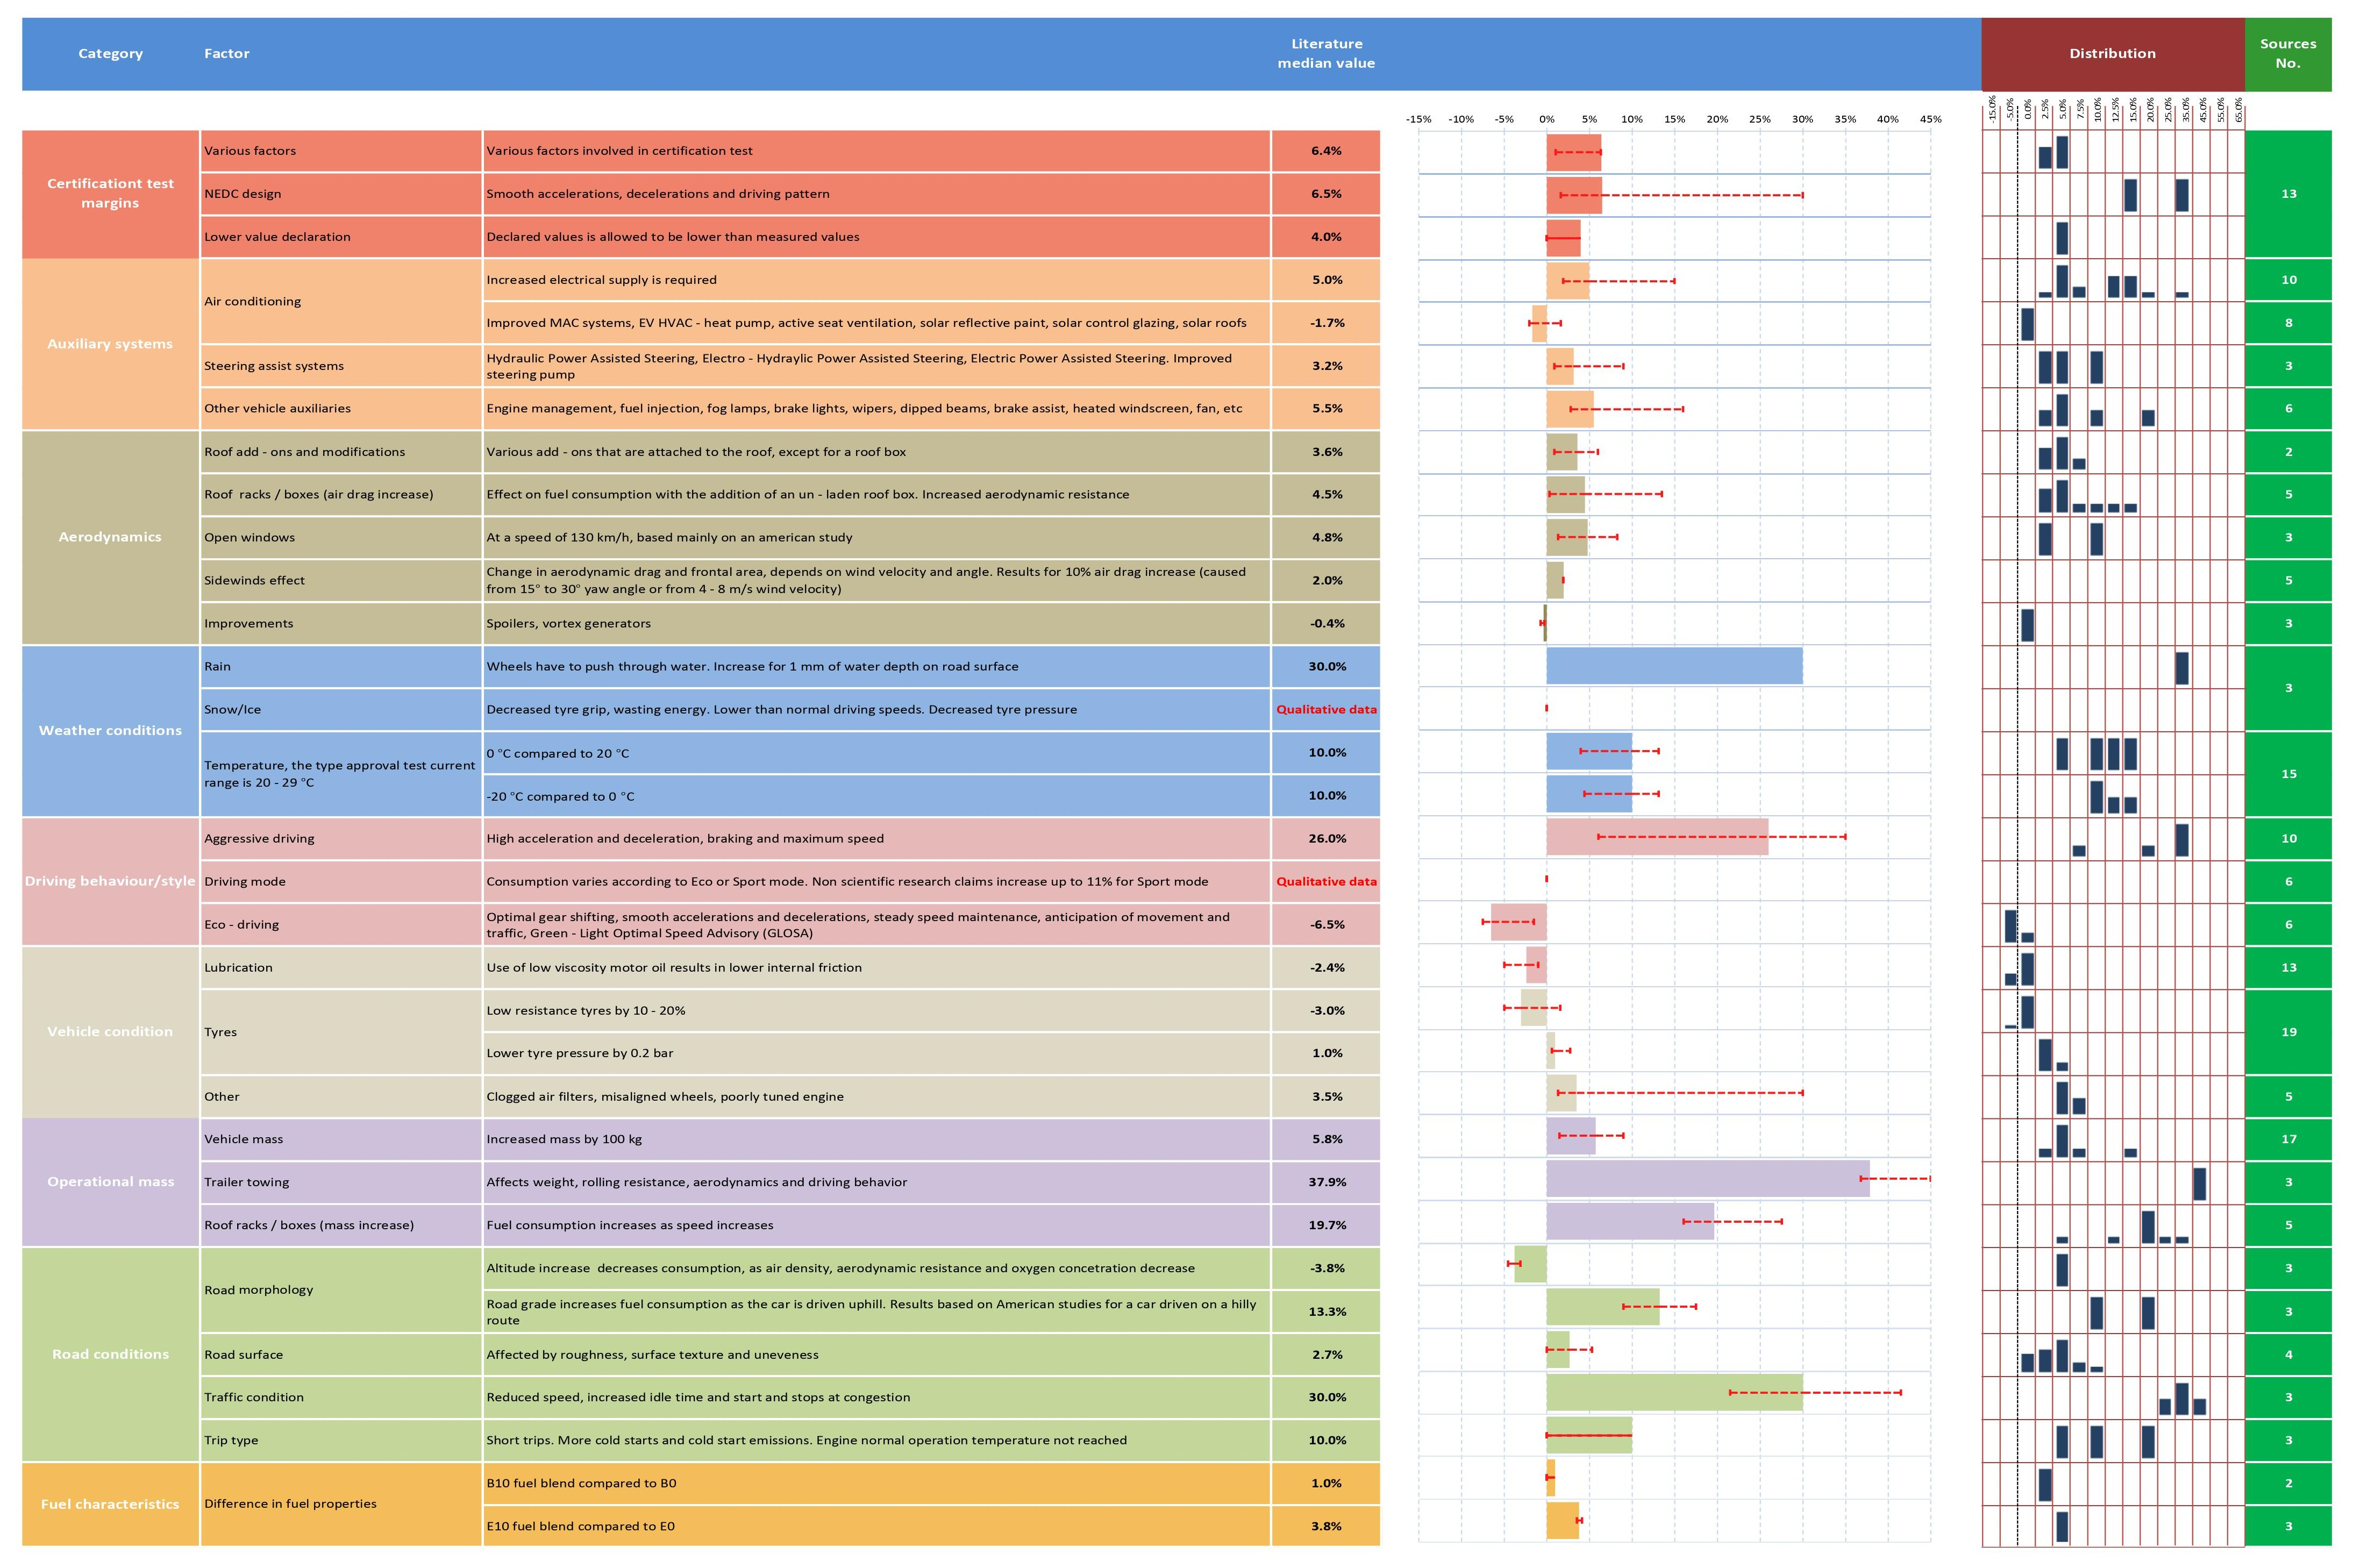
\includegraphics[width=0.95\columnwidth]{figures/factors_table.jpg}
  \caption{Fuel factors mentioned in the literature, together with the relative importance as reported by \parencite{zacharof2016review}}
  \label{table:ch2-sota-factors-table}
\end{sidewaysfigure}

Regarding driver-related factors, \hyperref[table:ch2-sota-factors-table]{Table} \ref{table:ch2-sota-factors-table} shows a group called \textbf{driving behaviour/style} that accounts for factors related directly to the driver. It is almost similar to the one from \hyperref[figure:ch2-sota-chart-factors]{Figure} \ref{figure:ch2-sota-chart-factors} with the exception of considering factors related to good driving styles that may reduce the fuel consumption.

Regarding the group \textbf{road conditions} in \parencite{zhou2016review}, it mainly includes the travel related, traffic related and roadway related factors.

Vehicle-related is the group with more factor's differences between both papers. Compared to \parencite{zhou2016review}, these factors are split into \textbf{auxiliary systems}, \textbf{vehicle conditions} and \textbf{fuel characteristics}, complemented with other groups that include factors related to the vehicle's design itself (\textbf{aerodynamics} and \textbf{operational mass}) and to \textbf{certification test margins}. In this last review, all these vehicle-related factors account for aspects related to the vehicle itself, not considering anything directly related to the driver. This is a difference when compared to the taxonomy of \parencite{zhou2016review}, because vehicle-related includes acceleration and speed factors.

The difference between the analyses shown in both articles are not only in terms of the taxonomy proposed to group factors, but sometimes also regarding the reported impact (i.e. exterior temperature has a median impact reported value of 10\% at \parencite{zacharof2016review} against the 1\% impact for all weather related causes reported by \parencite{zhou2016review}).

Within this last taxonomy of features that affect the fuel usage of a vehicle, some of them could be considered as "actionable", thus, they could be changed in a particular vehicle; in some cases without even needing to change the vehicle's route. An example of this is the aggressive driving style. Other features are inherent to the vehicle and cannot be directly changed, like the vehicle make/model or the vehicle mass. Even within the "actionable" features, some of them cannot be easily read through OBD-II (e.g., if there are roof add-on, which affects the vehicle aerodynamics). Thus, a subset of these features that considers only the ones that are "actionable" and the ones that can be read is the one shown in \hyperref[table:ch2-sota-FeatureInfluenceReduced]{Table} \ref{table:ch2-sota-FeatureInfluenceReduced}.

\begin{table}[]
\centering
 \begin{tabular}{c@{\qquad}c@{\qquad}c}
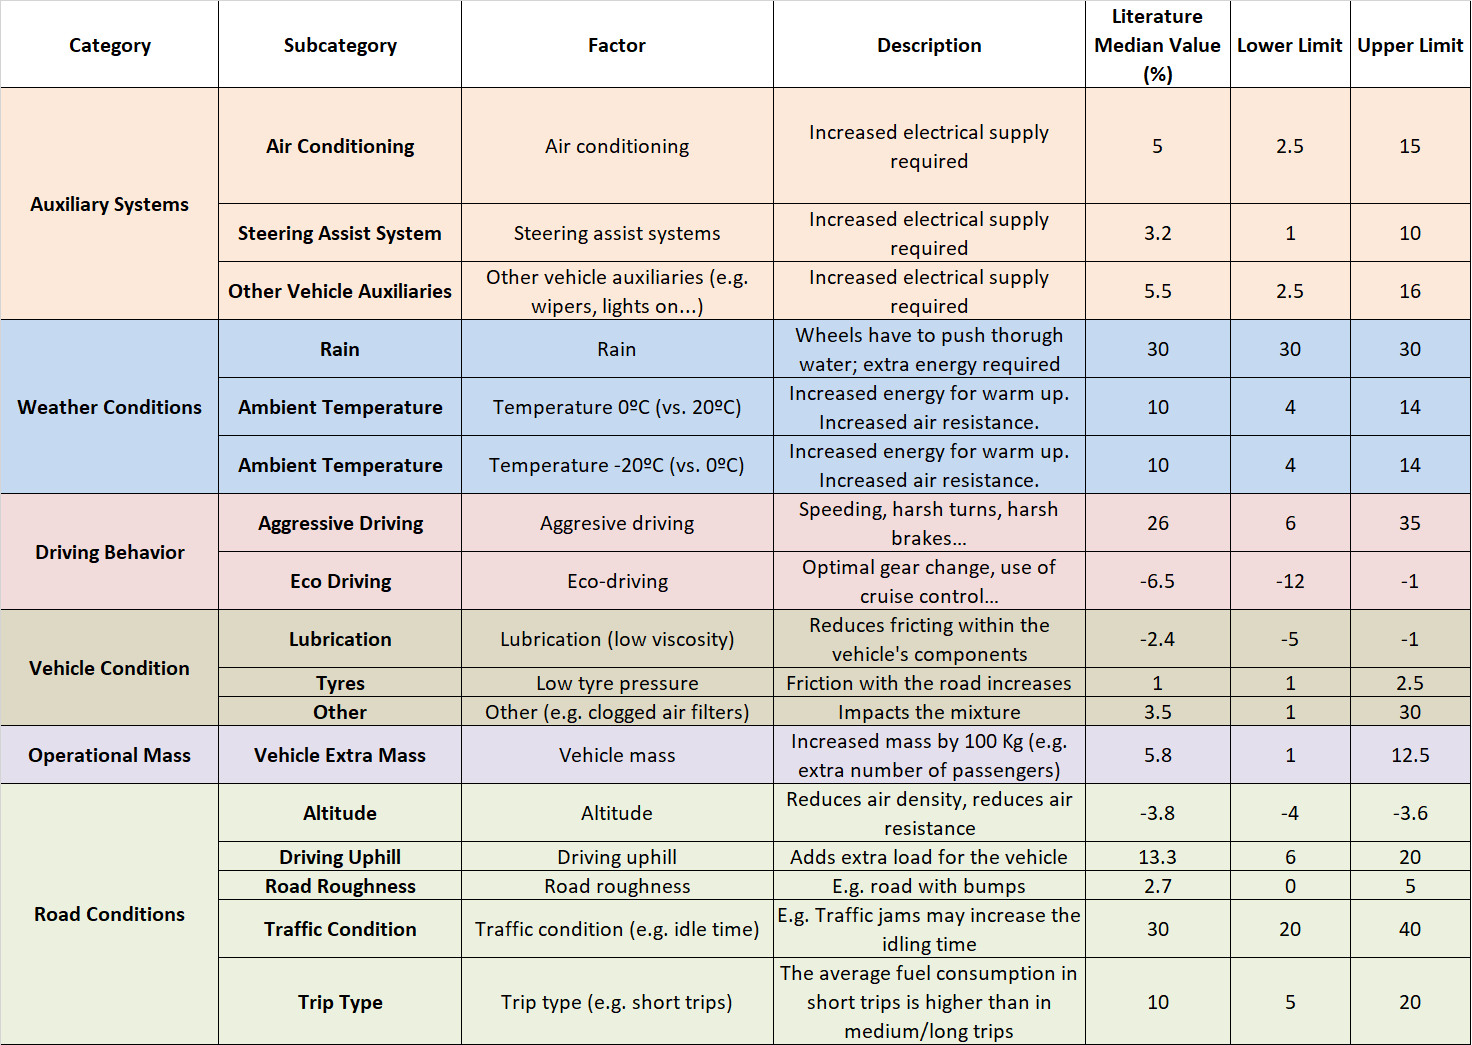
\includegraphics[width=0.90\columnwidth]{figures/FeatureInfluenceReduced.png}
  \end{tabular} 
  \caption{Reduced view from the factors of \parencite{zacharof2016review}, focusing on some of the actionable variables that can be retrieved from the OBD-II. The upper and lower limits refers to the minimum and maximum SOTA values reported in the review. For Rain, the lower limit is set to zero since the review does not provide limits for that feature. \label{table:ch2-sota-FeatureInfluenceReduced}}
\end{table}

The physical reasons as to why these features impact the fuel usage are:
\begin{itemize}
\item \textbf{Air conditioning (A/C)}: Using A/C increases the energy supply needed, leading to an increased fuel consumption. The time using the A/C and the power needed will increase/decrease that extra energy required. This category also includes the heating systems and related features, like the vehicle's coolant.
\item \textbf{Steering assist system}: These systems help driving safely and more confortable, but require additional electrical supply in exchange. An example is the usage of Electric power assisted steering (EPAS).
\item \textbf{Other vehicle auxiliaries}: These features include other auxiliary elements of the vehicle that may also require an extra energy. An example is the vehicle lights usage, that require extra energy and due to that, extra fuel.
\item \textbf{Rain}: Rain (and snow) impact the fuel usage in different ways. First, they affect the wheel gripping to the road surface. Also, the wheels have to push through an additional layer of water (or snow), so extra energy is required.
\item \textbf{Ambient temperature}: Temperature affects tyres, motor oil viscosity, cold start engine… Extra fuel is required in low temperatures to warm up the engine. It also affects aerodynamics: increased air density and higher aerodynamics resistances.
\item \textbf{Aggressive driving}: Aggressive driving is shown through different variables: acceleration patterns, gear change, harsh turns, harsh brakes, speeding... The impact on the fuel usage could be high.
\item \textbf{Eco driving}: Eco driving is related to the optimal driving of a vehicle, which may reduce its fuel usage. It involves optimizing the gear shifting (related to the usage of cruise control), choosing the best possible route thanks to a navigation device...
\item \textbf{Lubrication}: Overcoming of friction within the vehicle's components requires energy, and this is related to the fuel usage. If the friction is minimized thanks to an adequate lubrication, the energy required will be lower.
\item \textbf{Tyres}: Tyre pressure is related to the rolling resistance coefficient (RRC). When the tyres have low pressure, the contact surface with the road increases and more energy is needed to rotate the wheel (as the friction increases). 
\item \textbf{Other (vehicle condition)}: Beside tyres and lubricants, there are other vehicle conditions that impact the fuel usage. For instance, if the air filters are clogged. This is something that happens mainly in old models (since fuel injection in new cars is adjusted to ensure the correct mixture). Other examples are misaligned wheels and suspension losses. 
\item \textbf{Vehicle extra mass}: Extra mass in a vehicle (measured, for instance, in additional 100Kg), increase the energy needed to move the vehicle. This may happen for instance when there are additional passengers in a vehicle.
\item \textbf{Altitude}: In higher altitudes the air density is lower, so the air resistance that the vehicle faces while driving is also lower. This means that in higher altitudes the vehicle needs lower energy to move the same distance.
\item \textbf{Driving uphill}: Driving uphill adds an extra load over the vehicle, that needs additional energy to move. By contrast, driving downhill reduces the amount of energy needed.
\item \textbf{Road roughness}: For instance, if a road has many bumps, the vehicle will need additional energy to go through it. 
\item \textbf{Traffic condition}: Traffic condition also impacts in the fuel usage. For instance, if there are traffic jams, the idling time normally increases, leading to an increased average fuel consumption.
\item \textbf{Trip type}: The trip type also impacts in the fuel usage. For instance, if the trip distance is small, the average fuel consumption will increase, since fuel is required to turn on the vehicle.
\end{itemize}

There are some additional factors that impact in the fuel consumption that the previous references did not mention. This is the case of Diesel Exhaust Fluid (DEF). DEF is an urea-based product used in after-treatment processes of the vehicle, such as Selective Catalytic Reduction (SCR). It is applied over the vehicle's exhaust stream in order to transform the NOx gas emissions into nitrogen, water and CO2, reducing the NOx emissions in the process \parencite{betageri2016effects}. Techniques like SCR do not only reduce the emissions of a vehicle, but also help the engine performance and may lower fuel consumption \parencite{chen2015nonlinear, chen2013integrated}.

The factors already mentioned are linked to passenger vehicles, but for other vehicles, such as trucks, there are additional ones to consider. This is the case of power take-off, where there is power from the engine that is taken out (e.g. with a splined drive shaft) and used in another application (e.g. for a cement mixer in a truck). This directly impacts in the mileage of a vehicle \parencite{boriboonsomsin2010analysis}.

All these references show that there is a physical and empirically measured connection between the value of specific factors and the value of the fuel consumption. Thus, it is possible to use them in order to predict the value of the fuel consumption with ML models, as already shown within the literature \parencite{9072728, 8727915, perrotta2017application}.

\subsection{Machine Learning for connecting input features to vehicle fuel consumption}\label{subsec:ch2-sota-ml-fuel-consumption}
As we mentioned in the previous subsection, there are several features that affect the fuel consumption of a vehicle. This can be assessed using as input data source the feeds of data gathered from the vehicle's movement together with Machine Learning (ML) algorithms. This is the case of \parencite{ping2019impact}, where the authors conduct a study over a fleet of vehicles where they assess the impact of driving behaviour in the fuel consumption. They consider features related to driving behaviour, such as the gas pedal position, the speed and speed variance, or the steering angle, and they first see how those features have significant correlations with the fuel consumption. Then, they use several clustering algorithms (Spectral clustering, KFCM, K-Means), finding different clusters based on the driver consumption profile and its relationship with those driving behaviour features. 

In \parencite{perrotta2017application}, the authors analyse the impact of other features for fuel consumption within the context of trucks. The 56 features used include characteristics from the vehicle, such as its gross weight, together with others belonging to driving behaviour (usage of cruise control, average speed...), as well as information from the road (like the road surface macrotexture, or the curvature of the road). Those input features are seen as correlated with the fuel consumption (using a bivariate correlation analysis), and then are used to train several ML models (ANN, SVM, Random Forest) in order to predict the fuel consumption of the trucks. For the case of Random Forest, the authors viewed the relative impact from the different features in the fuel consumption through their contribution for accuracy during the tree splitting process.

The previous approaches are useful for detecting dependencies between a set of features and the fuel consumption of a vehicle. However, they do not quantify exactly how many extra liters of fuel are spent due to those features. In \parencite{andrieu2014evaluation}, the authors investigate the impact of eco-driving in the fuel consumption. Eco-driving is expressed through several features related to variables such as the Revolutions Per Minute (RPM) or the braking. Then, they use statistical tests for detecting significant decreases in fuel consumption when an eco-routing driving style is used. Then, they use a Logistic Regression model for analysing the relationship between driver-related features and the fact that the vehicle trip was actually done with eco-routing.

It is possible to use a Linear Regression model for measuring the individual impact of input features in fuel consumption, and know exactly how many liters are used due to each individual variable. The reason behind this is that those models are known as whitebox because they directly provide the influence of the input in the output \parencite{arrieta2020explainable}.
This is shown in \parencite{pavlovic2020understanding}, where the authors predict the fuel consumption gap between type-approval tests and real-world driving trips, using the information of one vehicle during one year, and with 20 different drivers. With that, they build a multiple linear regression model that takes into account driver-related factors as well as environmental and traffic factors in order to predict the fuel consumption gap. Through these linear models, they provide the relative importance for each of the features in the fuel consumption, as well as the r2 value for each of the models tested in order to evaluate them. Similarly, in  \parencite{lasocki2019environmental} the authors study the impact on the fuel of several features inferred related to driving behaviour through the analysis of the data from two different vehicles. One of these features is the Driving Style Indicator (DSI), which is the difference between the average positive acceleration of a vehicle minus the average of the negative acceleration divided by the average speed. The relationship between these features and fuel consumption is modeled through linear regression algorithms in order to quantify the impact of each one of them.

Even though linear regression models can be used for fuel prediction when there is a need of a whitebox ML algorithm that explains the relationship between input and output, this limits the results since the relationship inferred is linear. This problem can be solved by using non-linear whitebox models, such as Generative Additive Models (GAM). However, there is no literature to the best of our knowledge regarding the usage of these models for predicting vehicle fuel consumption.

\subsection{Anomaly detection for fuel consumption}\label{subsec:ch2-sota-anomaly-fuel}
The detection of anomalous fuel consumption in vehicles from a fleet is present at different research works within the literature. In \parencite{aquize2017self}, the authors show how to detect fuel anomalies using unsupervised algorithms (Self-Organizing Maps, SOM). The authors aim to find fuel fraud situations within fleet vehicle data at Bolivia (using a data set of 1000 vehicles with 190627 data points). These situations are normally linked to high fuel purchases within a short period of time. They effectively show how to find clusters within the space of the SOM to identify fuel anomalies and detect fraudulent scenarios by evaluating their proposal over a test set. As the authors mention, there are many features that can be used to contextualize the fuel consumption (e.g., the normal monthly consumption of the vehicle, the behaviour of other vehicles of the same subgroup...). Their proposal leads only to an output that identifies anomalies, but it could be greatly enhanced with XAI techniques that provide additional insights on what contextual features are relevant for that high fuel consumption.

Fuel fraud is not the only case of possible fuel anomalies within a fleet. As described in \parencite{zhang2017safedrive}, driving behaviour may also lead to an increased fuel consumption. Within driving behaviour variables, they mention several features, such as RPM speed, acceleration (both forward, and negative from braking), over speed or gear position.

Even though the previous literature includes research related to the detection of anomalous fuel consumption (both from fraud scenarios and from contextual variables), to the best of our knowledge there are no previous works regarding the explanation of those anomalies using XAI techniques.

\section{Summary}\label{sec:ch2-sota-summary}
In this chapter, we have seen the SOTA regarding XAI and unsupervised ML for anomaly detection, as well as XAI metrics for measuring the quality of explanations, and the combination of XAI with prior domain knowledge. We have also seen the SOTA for the use cases of this thesis: anomaly detection in network traffic, fuel factors that impact on the fuel consumption of petrol and diesel vehicles, and the usage of ML for either predicting fuel consumption or for detecting fuel consumption anomalies.

% Falta de evaluacion de XAI (con metricas) para el caso de modelos de deteccion de anomalias
Within our SOTA review, we detected a generalized lack of research regarding the evaluation of XAI explanations applied within the case of unsupervised anomaly detection. Indeed, the field of XAI metrics itself is still being actively researched, and most of the empirical studies regarding them focus on XAI for supervised ML models for classification and regression tasks, but not for unsupervised ML for anomaly detection, which is a very different task. 

% En el caso de stability/robustness, por ejemplo, solo hay propuestas para feature relevance pero no para rule extraction
% Metricas que faltan XAI
We also saw how even though there are several aspects that XAI metrics should measure (according to different taxonomies), the literature does not provide algorithms for measuring them. For some metrics, like \textbf{stability/robustness}, we saw that previous literature proposes metrics for feature relevance-based XAI techniques. However, there are no proposals, to the best of our knowledge, for other XAI techniques, such as rule extraction. Something similar happens with \textbf{diversity}, a metric which does not have any algorithmic implementation for XAI as far as we know.

% Falta de análisis del uso de domain knowledge con XAI en deteccion de anomalias para ajustar y evaluar las explicaciones, por lo que tiene sentido estudiarlo en un caso de uso real con el caso de fuel consumption.
The SOTA also indicates that even though XAI is useful for generating explanations about a model's decision, the explanations do not normally take into account causality aspects, so they can be misleading or directly incorrect. This is why combining XAI and prior domain knowledge is an important line of research for improving the quality and usefulness of explanations. However, this area is still relatively new, and there is no prior work as far as we know regarding anomaly detection within real-world contexts.

% Y mas metricas en este caso, como monotonicity degree
Related to that, the SOTA also shows that there is a need of XAI metrics that serve to not only compare techniques among themselves (like the aforementioned examples), but also against prior domain knowledge.

\newpage
    \chapter{Objectives and Contributions}\label{chap:3-objetives}

This chapter presents the objectives of this thesis along with the open research problems it addresses (\hyperref[sec:Objectives]{Section} \ref{sec:Objectives}), together with the main contributions (\hyperref[sec:Objectives]{Section} \ref{sec:Contributions}), the thesis assumptions, main and secondary hypotheses, and restrictions (Sections \ref{sec:Assumptions}, \ref{sec:Hypotheses}, \ref{sec:Restrictions}), in addition to the evaluation plan for the stated hypotheses (within \hyperref[sec:Hypotheses]{Section} \ref{sec:Hypotheses}). It concludes with the research methodology and process followed during the development of this thesis (\hyperref[sec:ResearchMethodology]{Section} \ref{sec:ResearchMethodology}).


\section{Problem statement and objectives}\label{sec:Objectives}
\textit{Is it possible to use Explainable AI (XAI) techniques for explaining the results of applying unsupervised learning algorithms for anomaly detection within real-world contexts?} This is a step towards designing industry products that follow Responsible Artificial Intelligence (RAI) by design principles regarding XAI. As real-world industry contexts, two use cases within the telecommunications industry are considered. 
The first one is related to communications data (e.g. calls received in a Call Center, mobile data usage), where the aim is to identify and explain daily anomalies. This use case appears within the software product of LUCA\footnote{The brand \textit{LUCA} has undertaken several changes due to business needs. Nonetheless, we will keep mentioning it within the product names for compliance with legacy documentations and references, in order to enhance clarity.} Comms \parencite{LUCAComms}.
The second one is related to vehicle fuel consumption, where the aim is to identify vehicles with anomalous diesel and petrol fuel consumption, explaining the potential reasons behind it. This use case appears within the software product of LUCA Fleet \parencite{LUCAFleet}.

To address the main thesis question, the following research problems and objectives need to be considered:

\mybox{
    \begin{itemize}
    \item[\textbf{P1.}] On many situations, anomalies must be detected in an unsupervised manner, because there is no prior information about them. However, the output of anomaly detection models is reduced to a binary decision, not explaining the reasons behind it.
    \end{itemize}
}

To tackle this problem, the following objective is defined:
\begin{itemize}
\item[\textbf{O1.}] Considering the binary output of an unsupervised learning algorithm for anomaly detection, apply a model-agnostic post-hoc XAI technique that explains the relationship between the output and the input features in terms of rule-extraction or feature relevance explanations.
\end{itemize}

\mybox{
    \begin{itemize}
    \item[\textbf{P2.}] Even though XAI can be used for understanding the decision of a black box model, there is a lack of quantitative metrics for evaluating the quality of the explanations and benchmarking the techniques that have been used.
    \end{itemize}
}

The objectives pursued for this problem is:
\begin{itemize}
    \item[\textbf{O2.1}] Define metrics that measure the quality of the explanations by themselves, with respect to several XAI aspects.
    \item[\textbf{O2.2}] Analyse whether the results from the application of different XAI techniques differ significantly from each other, and propose novel alternatives that are best suited for specific contexts.
\end{itemize}

\mybox{
    \begin{itemize}
    \item[\textbf{P3.}] Explanations directly generated by existing XAI techniques may contradict domain knowledge, making them useless while also reducing the user's trust in the algorithm behind. It is important to ensure and evaluate that they are aligned with that prior knowledge.
    \end{itemize}
}

For approaching this problem, we consider the two use cases, LUCA Fleet and LUCA Comms, since there is prior domain knowledge that can be taken into account. For both cases, we define a first common objective, where the domain knowledge and user expectations should be considered within the explanation generation. Then, since the domain knowledge of factors affecting fuel consumption is well-researched, we define additional objectives regarding how to measure the explanation quality against that prior domain knowledge, and if the explanations are indeed aligned or not.
Thus, the objectives are:
\begin{itemize}
    \item[\textbf{O3.1}] Propose an algorithm that adjusts the explanation generation considering the prior domain knowledge and user expectations within the use cases covered.
    \item[\textbf{O3.2}] Propose an approach for measuring the quality of the explanations with respect to a priori beliefs.
    \item[\textbf{O3.3}] Conduct a study to analyse whether the explanations provided are aligned with the previous State of the Art (SOTA) regarding factors affecting fuel consumption.
\end{itemize}

\mybox{
    \begin{itemize}
    \item[\textbf{P4.}] XAI explanations should be tailored for the specific profile of the user that will receive them, taking into account both their expectations and domain knowledge. This is something identified within the XAI theory, but there is a lack of real-world research that shows how to properly approach it.
    \end{itemize}
}

This problem will be addressed only within the context of LUCA Fleet since, in this case, there are different user profiles that receive explanations: fleet managers and fleet operators.
\begin{itemize}
    \item[\textbf{O4}] Identify the different user profiles that will receive explanations, and adjust the content according to them.
\end{itemize}

%\begin{itemize}
%\item[\textbf{P5.}] Despite the fact that RAI by design can be used for AI-based products (regarding XAI), %there is a lack of research within the use case of anomaly detection in real-world industry contexts.
%\end{itemize}

%This final problem will also be addressed within the context of both use cases, LUCA Comms and  LUCA Fleet, through the following objective:

%\begin{itemize}
%\item[\textbf{O5.}] 
%\end{itemize}

\section{Contributions}\label{sec:Contributions}

The scientific contributions from this thesis aim to provide answers to the research problems mentioned in \hyperref[sec:Objectives]{Section} \ref{sec:Objectives}. They are divided into two layers: the first layer highlights the main conceptual contributions, while the second layer provides the technical contributions behind them. 

Regarding the \textbf{main contributions} (first layer):

\begin{itemize}
\item[\textbf{C1 }] \textbf{HyperRulEx} (\textbf{Hyper}cube \textbf{Rule} \textbf{Ex}traction). A framework that standardizes several rule extraction algorithms through the usage of hypercubes, which can be applied over anomaly detection algorithms. The framework includes several XAI metrics for analysing quantitatively the quality of the explanations. This is described in \hyperref[chap:4-rule-extraction]{Chapter} \ref{chap:4-rule-extraction}.

\item[\textbf{C2 }] An \textbf{empirical study of XAI} applied for explanation generation from unsupervised learning \textbf{anomaly detection} algorithms over \textbf{real-industry data} considering \textbf{prior domain knowledge}. It includes \textbf{adjusting the explanations} according to both that domain knowledge, as well as the \textbf{user profile} that receives them. It also involves defining \textbf{metrics} that take into account that prior knowledge for the explanation evaluation. 
This study covers two use cases: communications data and vehicle fuel consumption, which leads to the following contributions.

    \begin{itemize}
    \item[\textbf{C2.1 }] An approach for extracting rule-based explanations for \textbf{visually explaining} anomalies within the context of communications data, considering \textbf{prior domain knowledge} for generating the explanations. This is described in \hyperref[chap:5-comms-xai]{Chapter} \ref{chap:5-comms-xai}.
    
    \item[\textbf{C2.2 }] \textbf{RESYFEX} (\textbf{Re}commender \textbf{Sy}stem for Vehicle \textbf{F}uel Saving based on \textbf{Ex}plainable AI). A Recommender System (RecSys) built with XAI by design, that explains \textbf{fuel consumption anomalies} considering \textbf{a priori expert domain knowledge}, adjusts those explanations for \textbf{different user profiles}, and provide \textbf{actionable recommendations} for vehicle fuel saving.  This is described in \hyperref[chap:6-fleet-xai]{Chapter} \ref{chap:6-fleet-xai}.
    
    \end{itemize}
\end{itemize}

Regarding the \textbf{technical contributions, TC,} (second layer), we divide them in three sections, depending on the main contribution that is associated to them.

For \textbf{C1}, the technical contributions are related to the development of the rule-extraction framework, along with the metrics for the algorithm evaluation. In particular, they are:

\begin{itemize}
\item[\textbf{TC1 }] \textbf{SVM+Prototypes reloaded}, an algorithm for generating both post-hoc global and local counterfactual \textbf{rule-based explanations} that are model agnostic. This algorithm is a variant from a previous one within the literature, and comes with two alternatives methods.
\item[\textbf{TC2 }] \textbf{StabilityScore}, an algorithm for measuring the \textbf{stability} of the explanations provided by rule-extraction XAI techniques.
\item[\textbf{TC3 }] \textbf{DiversityScore}, an algorithm for measuring the \textbf{diversity} of the explanations provided by rule-extraction XAI techniques.
\item[\textbf{TC4 }] A \textbf{metric} for quantifying several aspects for measuring the quality of explanations from rule-based XAI techniques into a single metric.
\item[\textbf{TC5 }] An \textbf{open source library} for (C1), that includes the algorithms from (TC1), (TC2), (TC3), and (TC4). 
\end{itemize}

Regarding \textbf{C2.1}, the technical contributions focus on how to adjust the explanations generated in order to take into account prior domain knowledge within a use case with communications data. In particular:
\begin{itemize}
\item[\textbf{TC6 }] An algorithm for generating \textbf{visual explanations} in terms of counterfactual limits from a surrogate model that has a binary output. It explains that output with respect to one numerical continuous feature and any number of categorical ones. 
\item[\textbf{TC7 }] A \textbf{hyperparamer grid search method} for \textbf{One-Class Support Vector Machine (OCSVM)} based on MIES (\textit{measure the distance from samples to enclosing surfaces}. It complements (C4) in order to ensure that the counterfactual limits that separate outliers from inliers only have one upper and one lower limit, so they anomalous data points are always above or below the inliers, but not between them.

\end{itemize}

Finally, \textbf{C2.2}, the technical contributions are related to the usage of XAI techniques for providing fuel saving recommendations. Thus, they focus on the adjustments of XAI algorithms for generating those recommendations considering prior domain knowledge, as well as adjusting them for different user profiles. In particular:
\begin{itemize}
\item[\textbf{TC8}] \textbf{EBM\_var}, a variation over \textbf{EBM algorithm} that adjusts the feature-based explanations to account for possible differences between data subgroups that correspond to combinations of categorical feature values.
\item[\textbf{TC9}] An algorithm for ensuring that the feature-relevance local explanations provided by EBM, or by (TC8) algorithm, are \textbf{monotonic}. It includes a metric for measuring the \textit{monotonicity degree} of the results.
\item[\textbf{TC10}] An algorithm that turns the feature-relevance based local explanations from interpretable ML models, using EBM, os (TC7), or Constraint GA2M plus (CGA2M+) as references, into \textbf{actionable recommendations}.

\end{itemize}

Within the context of \textbf{C2.2}, the contributions also include empirical contributions (EC) in order to quantitatively evaluate the XAI explanations against that prior domain knowledge. In particular:
\begin{itemize}
\item[\textbf{C14}] A study over the XAI proposals from (C2.2) in order to see if their impact in the fuel usage is aligned with the factors affecting the fuel consumption that the literature describes.

\end{itemize}


\section{Hypotheses}\label{sec:Hypotheses}
The main hypothesis is that XAI can be used for explaining the results of applying unsupervised learning algorithms for anomaly detection within real-world contexts. This hypothesis is split into the following sub-hypotheses:

\begin{itemize}
\item[\textbf{H1.}] It is possible to apply post-hoc model-agnostic XAI techniques for explaining the anomalies detected by an unsupervised learning algorithm, and quantitatively measure the quality of the explanations with the usage of XAI-specific metrics.

\item[\textbf{H2.}] It is possible to take into account prior domain knowledge along with XAI for anomaly detection, either for adjusting the explanations generated or for benchmarking the quality of the explanations against it.

% TODO - Comentario: ¿valdría simplemente con decir que 'se ha incluido la propuesta' en esos productos para validar H3, o mejor dejar sólo H1 y H2.
%\item[\textbf{H3.}] It is possible to use XAI within real-world industry products, following a RAI approach, for both detecting and explaining the anomalies detected. 
\end{itemize}

% Poner aquí un comment de las evaluations
% Duda: Un unico capitulo para el evaluation de todas las contribuciones? Busco como poder condensarlo en uno?
The hypotheses defined previously are evaluated within \hyperref[sec:RuleExtractionEvaluation]{Section} \ref{sec:RuleExtractionEvaluation}, \hyperref[sec:ch5-evaluation]{Section} \ref{sec:ch5-evaluation} and \hyperref[sec:ch6-evaluation]{Section} \ref{sec:ch6-evaluation}. \hyperref[fig:EvaluationPlan]{Figure} \ref{fig:EvaluationPlan} shows a schema for the Evaluation Plan (including only the principal contributions, C1, C2 and C3).


%\section{Evaluation Plan}\label{sec:EvaluationPlan}
%The hypotheses defined in Section \ref{sec:Hypotheses} are described below (see Chapter XXX for all the details of the evaluation performed). Figure \ref{fig:EvaluationPlan} shows a schema for the Evaluation Plan (including only the principal contributions, C1, C2 and C3).

%\begin{itemize}
%\item[\textbf{E1.}] (for H1) The goal of this evaluation is to use XAI techniques (focusing on rule extraction and feature relevance) and apply them over unsupervised learning algorithms for anomaly detection, approaching them as a classifier with a binary output. The evaluation includes the usage of already existing and novel XAI metrics in order to benchmark the explanations provided. Thus, we can compare several techniques, and see if there are differences depending on the context, even though the techniques themselves are model agnostic.

%\item[\textbf{E2.}] (for H2) The goal of this evaluation is, to first elicit domain specific knowledge and user's expectations for the explanations, and use that information for adjusting the explanations generated by the XAI techniques considered, within the context of LUCA Comms and LUCA Fleet. For LUCA Fleet, the evaluation includes the usage of metrics related to the prior domain knowledge in order to see if the explanations regarding potential fuel saving are aligned. 

%\item[\textbf{E3.}] (for H3) The goal of this evaluation is to determine whether it is possible or not to develop a product following RAI principles (regarding XAI) that successfully detects and explains the anomalies detected by unsupervised models.
%\end{itemize}

\begin{sidewaysfigure}[h!]
  \centering
  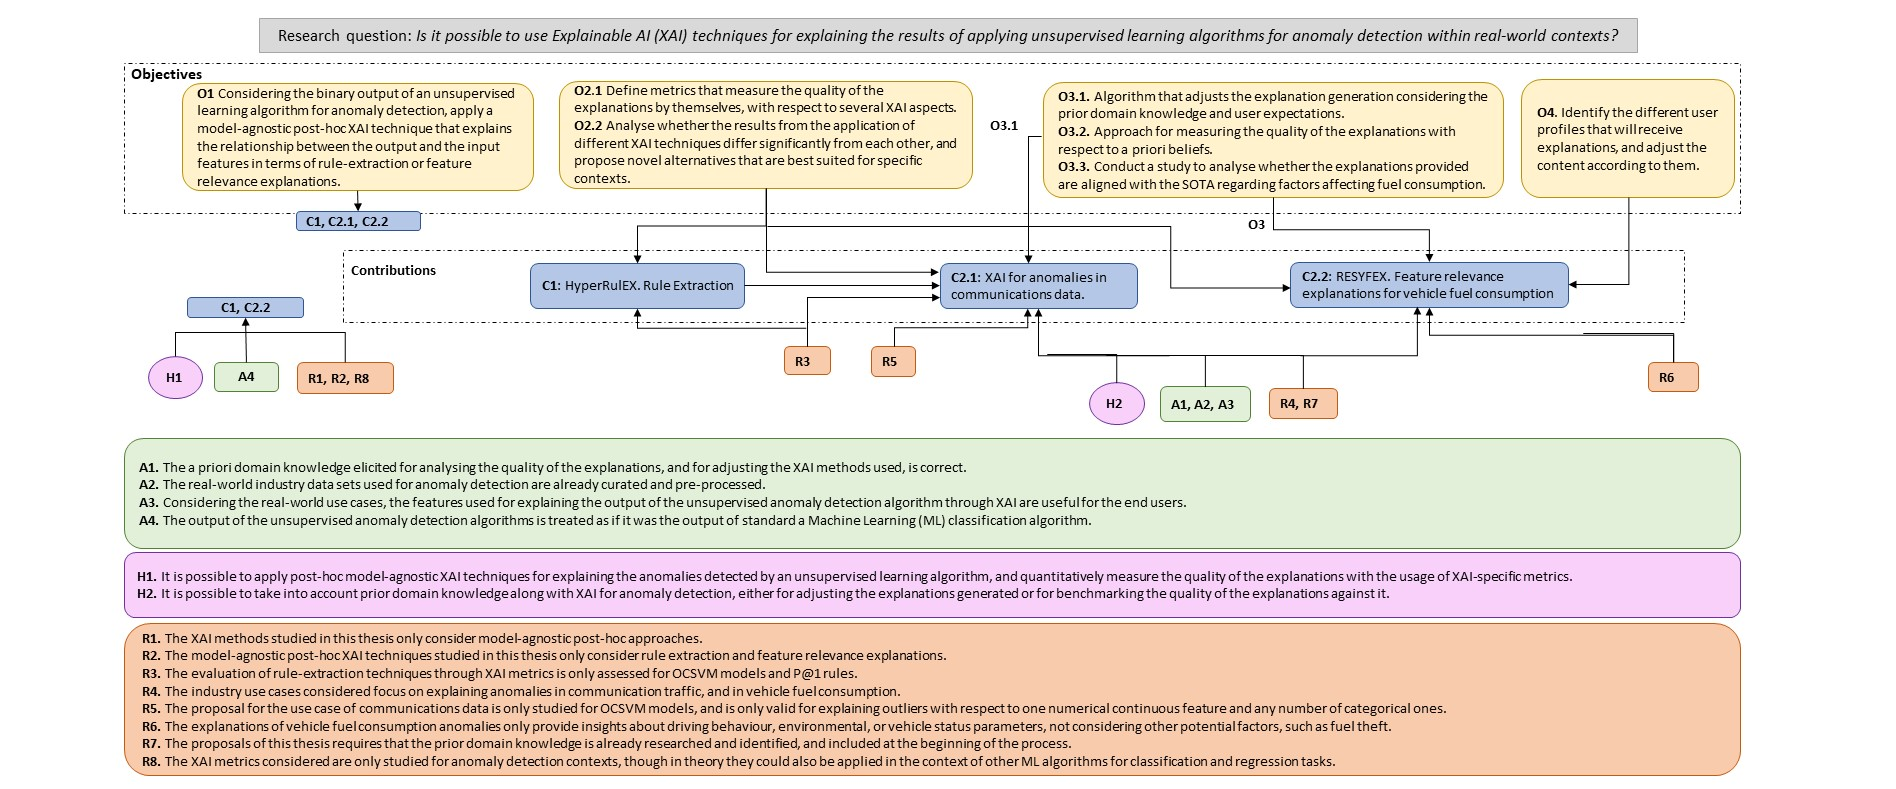
\includegraphics[width=0.85\columnwidth]{figures/EvaluationPlan.jpg}
  \caption{Relations between objectives, contributions, hypotheses, restrictions and assumptions of this thesis.}
  \label{fig:EvaluationPlan}
\end{sidewaysfigure}

\section{Assumptions}\label{sec:Assumptions}
This thesis was developed under a set of assumptions that help to explain the decisions taken for the achievement of the thesis goals; such assumptions are listed below:

\begin{itemize}
\item[\textbf{A1.}] The a priori domain knowledge elicited for analysing the quality of the explanations, and for adjusting the XAI methods used, is correct.

\item[\textbf{A2.}] The real-world industry data sets used for anomaly detection are already curated and pre-processed, eliminating noisy registers (e.g. sensor measurement errors). They also contain the most relevant features for explaining the potential outliers.  

\item[\textbf{A3.}] Considering the real-world use cases, the features used for explaining the output of the unsupervised anomaly detection algorithm through XAI are useful for the end users that are receiving them.

\item[\textbf{A4.}] The output of the unsupervised anomaly detection algorithms is treated as if it was the output of standard a Machine Learning (ML) classification algorithm.

% TODO - Comment: ¿Cómo que esta es 'strong'? ¿La quito, la dejo o la modifico?
%\item[\textbf{A4.}] The empirical metrics used for measuring the quality of the different types of explanations generated are assumed to be correct based on the previous literature.

\end{itemize}

\section{Restrictions}\label{sec:Restrictions}
The following restrictions define boundaries of the contributions of this thesis, highlighting future research problems than can be further pursued. These restrictions are:

\begin{itemize}
\item[\textbf{R1.}] The XAI methods studied in this thesis only consider model-agnostic post-hoc approaches.

\item[\textbf{R2.}] The model-agnostic post-hoc XAI techniques studied in this thesis only consider rule extraction and feature relevance explanations. Other alternatives, such as prototype-based explanations, are not researched.

\item[\textbf{R3.}] The evaluation of rule-extraction techniques through XAI metrics is only assessed for OCSVM models and P@1 rules.

\item[\textbf{R4.}] The industry use cases considered focus on explaining anomalies in communication traffic, and in vehicle fuel consumption. However, other use cases could be considered.

\item[\textbf{R5.}] The proposal for the use case of communications data is only studied for OCSVM models, and is only valid for explaining outliers with respect to one numerical continuous feature and any number of categorical ones.

\item[\textbf{R6.}] The explanations of vehicle fuel consumption anomalies only provide insights about driving behaviour, environmental, or vehicle status parameters, not considering other potential factors, such as fuel theft.

% No entiendo muy bien el comment the Oscar. Por que poner lo de 'independently of where it is taken from'? Lo que quiero decir aqui es que tiene que estar identificado e incluido desde el ppio.
\item[\textbf{R7.}] The proposals of this thesis requires that the prior domain knowledge is already researched and identified, and included at the beginning of the process.
%The domain knowledge considered for the use cases in this thesis is already well-researched within the previous literature, so the proposed solution includes it from the beginning, instead of gathering it from the end users. 

\item[\textbf{R8.}] The XAI metrics considered are only studied for anomaly detection contexts, though in theory they could also be applied in the context of other ML algorithms for classification and regression tasks.

\end{itemize}


\section{Research methodology}\label{sec:ResearchMethodology}
This section presents an overview of the research methodology followed during this thesis. To achieve the contributions related to the research problems described in \hyperref[sec:Objectives]{Section} \ref{sec:Objectives}, several methodology phases are defined, as indicated in \hyperref[fig:ResearchMethodologyFigure]{Figure} \ref{fig:ResearchMethodologyFigure}. Along with the phases, the figure depicts the activities carried out, and the contributions generated in each of those phases. The contributions are indicated though the appropriate bibliographic references.


\begin{itemize}

\item[1.] \textit{Domain Research Work.} An analysis of RAI is conducted, highlighting the importance of including XAI aspects during the design phase of AI-based products. As a result, we saw that this development approach was still an open area within real-world industry products. Because of that, we focused on applying it within two real-world industry products: LUCA Comms and LUCA Fleet.

\item[2.] \textit{Survey.} We conducted a review of the SOTA of both XAI and RAI, finding that even though there are many contributions for supervised ML models, there are areas where more research is needed. One of those areas is studying the applicability of XAI to unsupervised anomaly detection algorithms. We also saw a lack of research for XAI applied to anomaly detection within real-world industry use cases. Finally, we also discovered that the usage of quantitative metrics for assessing the quality of the explanations needed more research.

\item[3.] \textit{Development.} We first focused on studying rule extraction based techniques, since there was a lack of metrics regarding the measurement of the quality of the explanations. With this, we proposed a framework that standardizes the rule-extraction methods, and measures the quality of explanations with XAI metrics (C1). We then took the rule extraction approach for the use case of LUCA Comms, where the explanation generation needed to be adjusted in order to consider user's expectations and prior knowledge, leading to (C2.1). We also considered a third XAI approach by using feature relevance based techniques, and applying them within the context of vehicle fuel consumption (LUCA Fleet), leading to (C2.2), where the explanations generated must take into account prior domain knowledge. Within this last real-world use case, we also conducted an analysis in order to see if the final explanations are aligned with other aspects within the prior domain knowledge.

\item[4.] \textit{Implementation.} The three XAI approaches considered for explaining the output of anomaly detection algorithms lead to different final results and implementations. 
With (C1), an open source library was developed, providing a common framework for rule extraction, including XAI metrics for analysing the explanation quality. For (C2.1), the proposal is integrated within LUCA Comms product. Finally, for (C2.2), a fuel saving recommender system was developed, leading to a software prototype that is going to be included within LUCA Fleet in a future release.
\end{itemize}

\begin{figure}[h!]
\centering
  \begin{tabular}{c@{\qquad}c@{\qquad}c}
  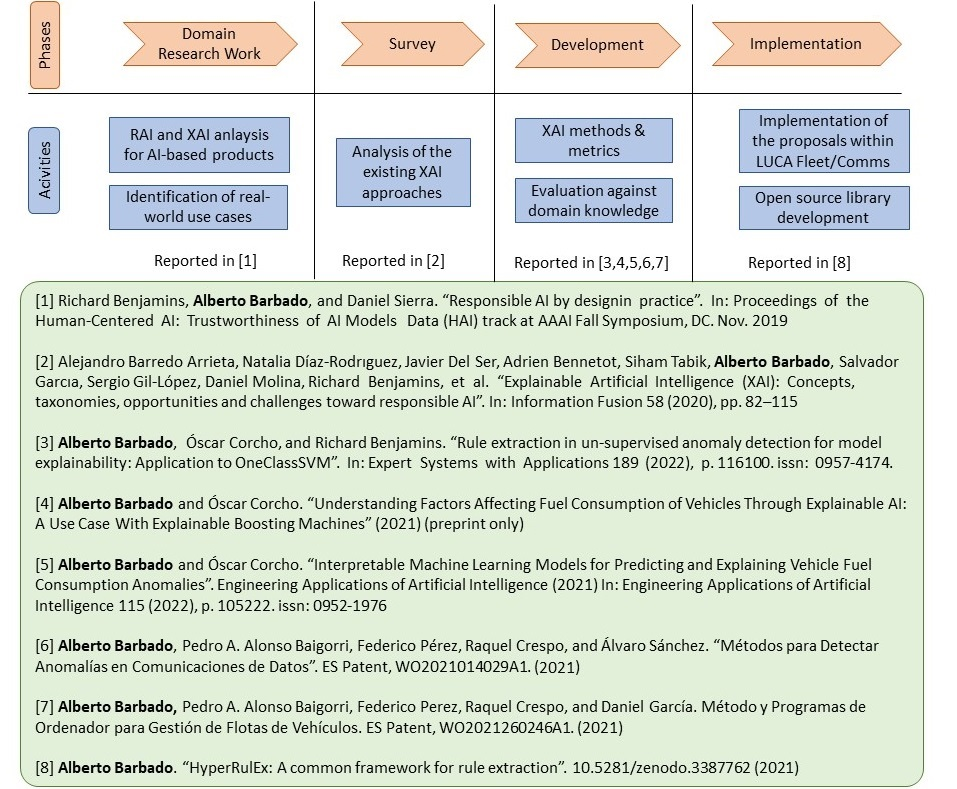
\includegraphics[width=0.9\columnwidth]{figures/ResearchMethodology.jpg}
  \end{tabular} 
  \caption{Phases of the thesis development, including the activities carried out during
each phase and the main publications derived from each phase.}
  \label{fig:ResearchMethodologyFigure}
\end{figure}


\newpage
    \chapter{Explainable Anomaly Detection with Rule Extraction Techniques: A Framework for Generating and Evaluating Explanations Over Unsupervised Machine Learning Models}\label{chap:4-rule-extraction}

In this chapter, we present our first contribution \textbf{C1} for extracting and evaluating rule extraction-based explanations obtained using Explainable Artificial Intelligence (XAI) techniques over unsupervised Machine Learning (ML) algorithms for anomaly detection, as discussed in \hyperref[sec:Hypotheses]{Section} \ref{sec:Hypotheses}. The main content of this chapter appears in in our published paper \parencite{barbado2022rule}.

The work presented in this chapter addresses hypothesis \textbf{H1} from \hyperref[sec:Hypotheses]{Section} \ref{sec:Hypotheses}, which states that it is possible to use metrics for measuring the quality of the XAI explanations within the context of unsupervised learning algorithms for anomaly detection. We first justify mathematically how it is possible to measure different XAI explanations aspects from rule extraction methods. Then, we carry out an empirical analysis within the context of unsupervised learning for anomaly detection, where we see that thanks to XAI metrics we can find rule extraction methods that are more suitable for this specific context, obtaining better metric values with some methods compared to others. This is helpful for seeing that even if the XAI methods are \textit{model-agnostic}, the explanations generated are significantly influenced by the context.

We divide this chapter in six sections. \hyperref[sec:RuleExtractionIntroduction]{Section} \ref{sec:RuleExtractionIntroduction} introduces the problem and gives the context for our proposals. \hyperref[sec:RuleExtractionVariants]{Section} \ref{sec:RuleExtractionVariants} presents our rule extraction XAI algorithm variants. \hyperref[sec:RuleExtractionMetrics]{Section} \ref{sec:RuleExtractionMetrics} shows the XAI algorithm metrics considered for analysing the quality of the explanations, including our novel algorithm proposals for several of them. \hyperref[sec:RuleExtractionFramework]{Section} \ref{sec:RuleExtractionFramework} proposes our framework to standardize rule extraction techniques in order to have a common output for obtaining the XAI metrics and evaluating the explanations. In \hyperref[sec:RuleExtractionEvaluation]{Section} \ref{sec:RuleExtractionEvaluation} we present the empirical evaluation carried out with our proposal. Finally, \hyperref[sec:RuleExtractionConclusion]{Section} \ref{sec:RuleExtractionConclusion} presents a summary of the conclusions for this chapter.

%There are several Explainable Artificial Intelligence (XAI) techniques for extracting rule-based explanations that are model-agnostic, so they can be applied to unsupervised ML algorithms for anomaly detection that yield a binary output. However, the explanations yielded may differ significantly, and some of the may be more suitable for anomaly detection context, where P@1 explanations gain more relevance with respect to other domains. Because of that, we focus on an already-existing algorithm proposal that is intuitively more suitable for P@1, and we propose some variations over that algorithm in order to specifically improve the results within this context. We also propose novel algorithm for computing several XAI metrics in order to assess the quality of the explanations from a quantitative point of view. Finally, we present a framework that standardizes rule extraction-based model-agnostic post-hoc XAI techniques in order to be able to obtain the same XAI metrics for all of them, so the explanations can be benchmarked.

\section{Introduction}\label{sec:RuleExtractionIntroduction}
Anomaly detection is one of the tasks for which unsupervised learning techniques can be applied. It is defined as the process of detecting anomalous observations within a data set, and sometimes remove it as a first step within data-mining applications \parencite{hodge2004survey}. There is often no prior information about outliers in a data set, hence unsupervised ML algorithms offer the chance to infer patterns and detect potential anomalies. However, not only is it important to detect outliers, but also to explain why they are outliers\footnote{We use the term 'outliers' as a synonym for 'anomaly', since the literature sometimes uses them interchangeably}. Explanations can help to understand why a particular data point has been labelled anomalous (and what changes in the feature values would lead to classify it as an inlier), and how the model behaves globally (for instance, what features influence more for classifying a data point as an outlier).

The output of an unsupervised ML model for anomaly detection can be seen as binary (an observation may be an \textit{outlier} or an \textit{inlier}). Thus, surrogate post-hoc XAI techniques can yield explanations similarly to a supervised binary classifier where the two possible outputs are imbalanced. Hence, the explanations for the model can be obtained by using XAI techniques already designed for supervised ML binary classifiers. This is already addressed in the literature, as we discussed in \hyperref[sec:ch2-sota-xai-anomaly-detection]{Section} \ref{sec:ch2-sota-xai-anomaly-detection}, particularly by using feature-relevance XAI techniques \parencite{ruff2021unifying, langone2020interpretable}.

Among the different model-agnostic post-hoc XAI techniques that can be applied, rule extraction offers the possibility to provide both global and local explanations, as indicated by the recent literature \parencite{arrieta2020explainable}. This is achieved by using an "IF...THEN" schema that explains both the output of a particular data point as well as the global behaviour of the original model. In the case of anomaly detection, they can explain both a particular outlier and also how the features of the whole model contribute to identify points as outliers or inliers. Even though there are some examples of this in the literature, particularly for the case of One-Class SVM (OCSVM) \parencite{padmaja2015hybrid}, there are not many studies covering it to the best of our knowledge.

There is a particularity of the usage of rule extraction for explaining anomalies. An anomaly detection system that uses rules as explanations may have more interest in explaining faithfully why a data point is an outlier, and what should have happened to consider it an inlier, rather than being able to cover all possible scenarios with explanations that may be wrong. This means that the extracted rules need to have a very high precision (P@1); rules that classify data points from one class (i.e. "outliers") without including data points from the other one. Considering the example of rules extracted that cover inliers, this is important because the counterfactual explanation for turning an outlier into an inlier should lead to a scenario where the model will always classify it as an inlier.

This is linked to another aspect regarding XAI. Even though there are many model-agnostic post-hoc rule extraction techniques that can be used for explaining a ML model in general, with some of them applicable even for unsupervised anomaly detection in particular, there is still one question present: which technique provides the best explanations?. This leads to an open issue within the XAI literature: how to evaluate the quality of explanations?. Here, the literature suggests some concepts to consider while designing new metrics and algorithms, as discussed in \hyperref[sec:ch2-sota-xai-anomaly-detection]{Section} \ref{sec:ch2-sota-xai-anomaly-detection}. The metrics need to consider the type of explanations provided (rule based in this case) and the type of data used. In our case, we work on anomaly detection without a prior ground truth. Hence, some XAI metrics (like those related to accuracy measurement of the rule predictions over a test set) are not applicable. Together with that, other particularities of the problems addressed may influence which metrics are more important. Considering P@1 rules, measuring the fidelity of the explanations is not necessary (since the comparison will only be possible against the model output). However, other metrics gain more relevance, such as stability. With that, some relevant aspects to measure for this case are: 

\begin{itemize}
\item \textbf{Comprehensibility}: Are explanations easy enough to understand?
\item \textbf{Representativeness}: Are explanations relevant? Do they explain all possible cases?
\item \textbf{Stability}: Do explanations match the predictions of the model? Or are there inconsistencies?
\item \textbf{Diversity}: Are explanations sufficiently different among them? Or are they redundant?
\end{itemize}

This highlights that, even though model-agnostic rule extraction XAI techniques can be applied over the results of an unsupervised ML algorithm for anomaly detection from a technical point of view, the results (explanations) may differ when comparing the different techniques. With this, we focus on addressing and proposing methods that may be more suitable for the specific case of anomaly detection and for P@1 rules, as well as presenting metrics for evaluating and comparing the explanations.

\section{Rule extraction algorithm variants}\label{sec:RuleExtractionVariants}
In this section, we describe the intuition behind our proposals for variants of some already-existing rule extraction algorithms. The detailed description of the algorithms appear in \hyperref[sec:annex-rule-extraction]{Section} \ref{sec:annex-rule-extraction} within the \hyperref[ch:annex]{Annex}.

\subsection{Algorithm intuition}\label{subsec:RuleExtractionAlgorithmIntuition}
We propose using rule extraction techniques within OCSVM models for anomaly detection, by generating hypercubes that encapsulate the non-anomalous data points, and using their vertices as rules that explain when a data point is considered non-anomalous.

The work of \parencite{nunez2002rule} proposes an algorithm to extract rules from a SVM model by performing clustering over the data points that belong to one of the classes. The clustered data points will be used to obtain a geometric surface that encloses the rest of the data points inside. There are two ways to accomplish it: building hypercubes or building hyperspheres. We focus the analysis over the first approach: building hypercubes. We also focus in the model-agnostic variant, where the algorithm obtains the furthermost data points from inside the cluster as vertices for the hypercube, so they enclose the rest of data points of that category inside (the model specific alternative uses the support vectors). In case that the hypercube generated encloses points from the other category, then the number of clusters will be increased, aiming to obtain smaller cubes that could fit the data without including points from the other class. This is done iteratively until no points from the other class are inside the hypercubes, or a maximum number of predefined iterations is reached. During the process, if a hypercube does not contain points from the other class, then that hypercube is translated into a rule, and those data points are removed from the following iteration steps.

Figures \ref{fig:ch4-starting-point} and \ref{fig:ch4-discard} show an example application of this algorithm for a 2D space. \hyperref[fig:ch4-starting-point]{Figure} \ref{fig:ch4-starting-point} shows the initial scenario, where the first step in the iteration process consists in applying one cluster over the data set for data points of one of the classes (blue ones). However, with one cluster, the 2D square that encloses the data points contains points from the other class, so more clusters need to be applied. As \hyperref[fig:ch4-discard]{Figure} \ref{fig:ch4-discard} shows, iteration 3 (with 3 clusters) is the first one with squares without red points, so those subspaces are turned into rules and the points inside them removed from the iteration process, that starts again with one cluster for the remaining data points. Iteration 6 will be the last one, and 5 rules have been extracted up to that point.

\begin{figure}[!h]
\centering
  \begin{tabular}{c@{\qquad}c@{\qquad}c}
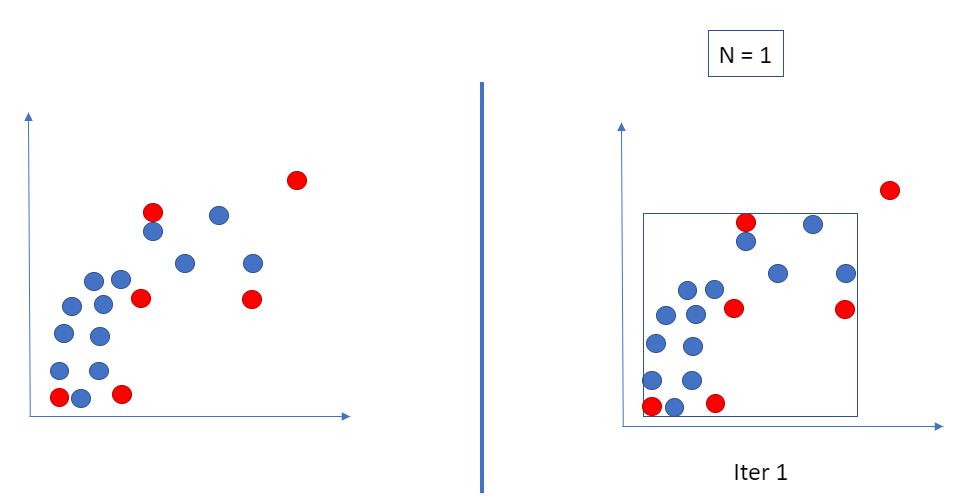
\includegraphics[width=0.7\columnwidth]{figures/chapter4_RuleExtraction/start.png}
  \end{tabular} 
  \caption{Clustering over a 2D space. With one cluster over data points from one class (blue), there are still others from the other class (red) inside the square.\label{fig:ch4-starting-point}}
\end{figure}

\begin{figure}[!h]
\centering
  \begin{tabular}{c@{\qquad}c@{\qquad}c}
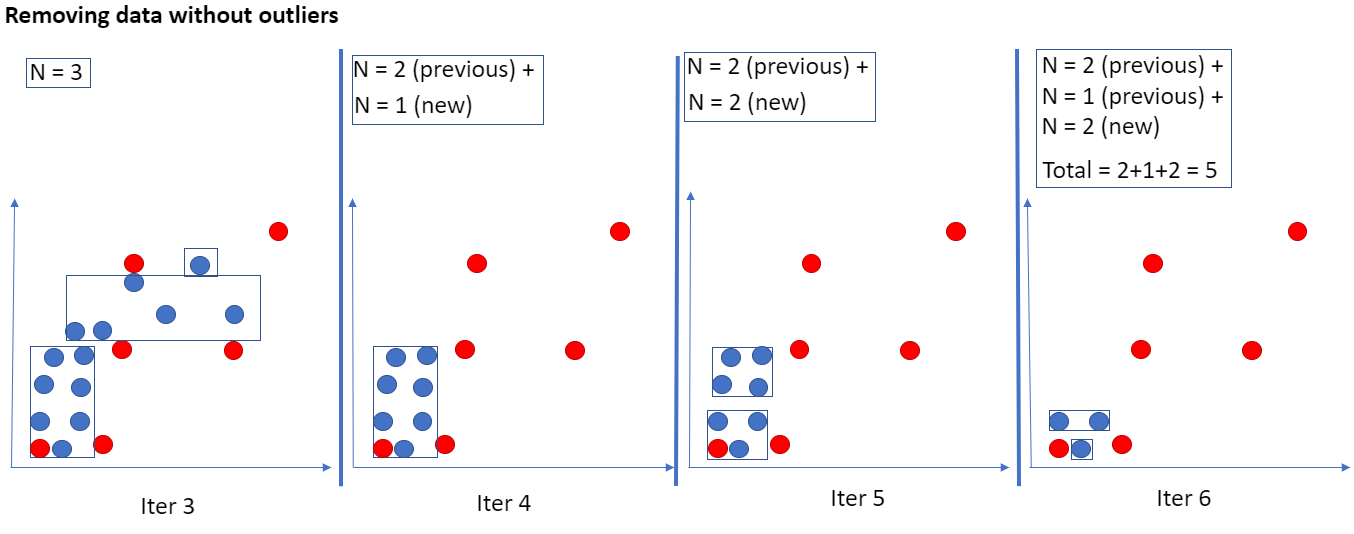
\includegraphics[width=0.8\columnwidth]{figures/chapter4_RuleExtraction/discard.png}
  \end{tabular} 
  \caption{Applying the proposal of \parencite{nunez2002rule}, the number of clusters keeps increasing until no points from the other class are inside, an then that hypercube is translated into a rule.\label{fig:ch4-discard}}
\end{figure}

The approximation proposed before is not the only one that can be applied in order to extract the rules. \hyperref[fig:ch4-keep]{Figure} \ref{fig:ch4-keep} shows one of our alternative proposals over \parencite{nunez2002rule} method. Instead of removing data points that are inside a rule without points from the other class, the process always keeps all data points in every iteration since there could be clustering patters that could only be found if all points are together. In this approach, the number of clusters is constantly increased until no data points from the other class are inside the hypercubes, or the maximum number of iterations is reached. We will further address this method as \textbf{keep} in the remaining of the chapter. In contrast, the references to \parencite{nunez2002rule} method will be addressed as \textbf{keep\_reset}.

\begin{figure}[!h]
\centering
  \begin{tabular}{c@{\qquad}c@{\qquad}c}
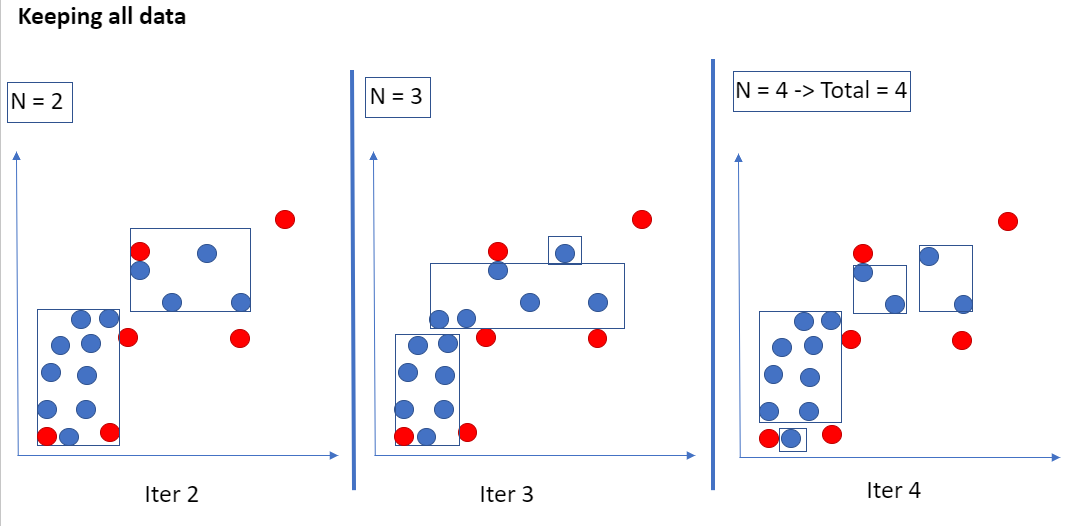
\includegraphics[width=0.75\columnwidth]{figures/chapter4_RuleExtraction/keep.png}
  \end{tabular} 
  \caption{Keeping all data points in every iteration could lead to a reduced number of clusters since there may be data patterns that could only be found in this scenario. \label{fig:ch4-keep}}
\end{figure}

Another proposal that we include in this chapter over \parencite{nunez2002rule} is splitting the subspaces in a binary partition scheme. This is an alternative over the original proposal, that constantly increases the number of clusters until one rule has only data points from the same class, and then restarting the clustering process from the beginning for the remaining ones. We will address this method as \textbf{split} for the remaining of the chapter. \hyperref[fig:ch4-keep-reset]{Figure} \ref{fig:ch4-keep-reset} shows how the same 2D example using this approach.

\begin{figure}[!h]
\centering
  \begin{tabular}{c@{\qquad}c@{\qquad}c}
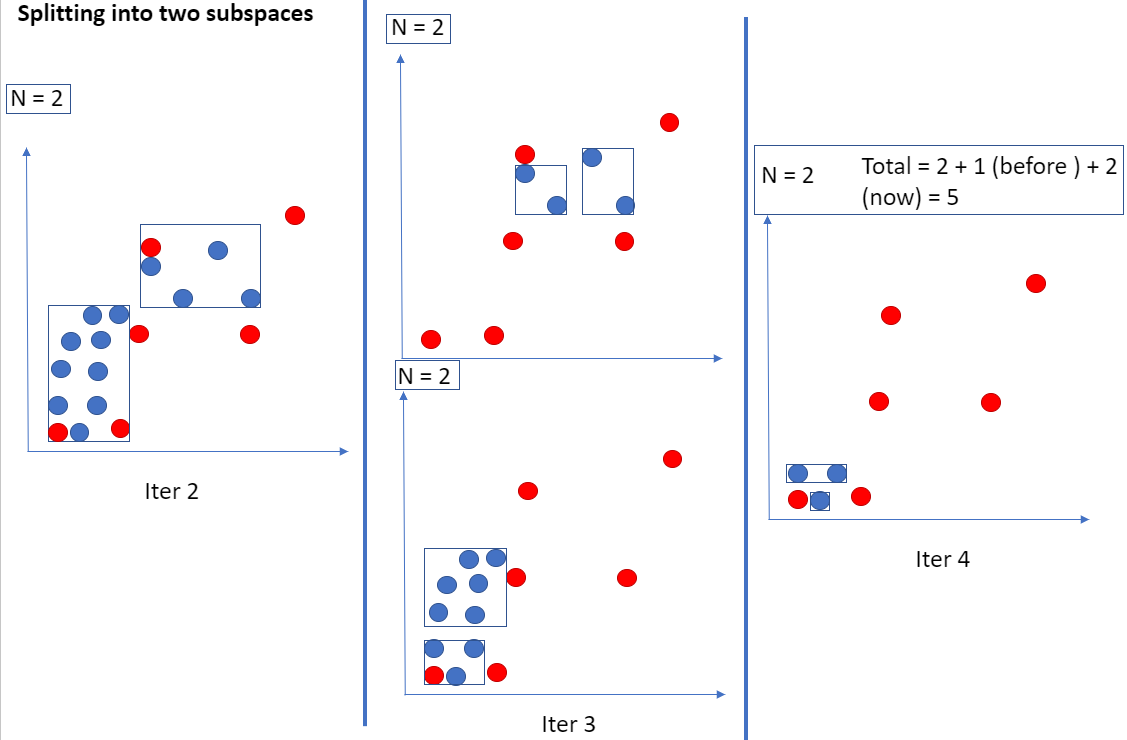
\includegraphics[width=0.7\columnwidth]{figures/chapter4_RuleExtraction/keep_reset.png}
  \end{tabular} 
  \caption{Splitting subspaces with a binary partition scheme until no red points are inside the rule. \label{fig:ch4-keep-reset}}
\end{figure}

According to the taxonomy for XAI in \parencite{molnar2019interpretable}, our method has the following characteristics:
\begin{itemize}
    \item \textbf{Post-hoc}: Explainability is achieved using external techniques.
    \item \textbf{Global and individual}: Explanations serve to explain how the whole model works, as well as why a specific data point is considered anomalous or non-anomalous.
    \item \textbf{Model-agnostic}: As with other techniques for global explanations \parencite{molnar2019interpretable}, the only information needed to build the explanations are the input features and the outcomes of the system after fitting the model.
    \item \textbf{Counterfactual}: The explanations for why a data point is anomalous also include information on the changes that should take place in the feature values in order to consider that data point as non-anomalous.
\end{itemize}

Since the explanation algorithm is model-agnostic, it can work for any blackbox model. The only information needed is the train data set and the outputs from the model.  To illustrate it, we show evaluations over OCSVM models with different kernels: radial basis function (RBF) and linear kernel.

Regarding the clustering technique itself, potentially any algorithm could be used, both for \parencite{nunez2002rule} or for any of out two proposals over it from this chapter. However, there is a caveat that should be considered. The clustering algorithm needs to take into account if the features are only numerical, categorical (non ordinal), or both. 

One algorithm that will be used in this chapter for extracting the hypercubes is K-Means ++ \parencite{arthur2006k}. However, the standard version of this clustering algorithm is designed for numerical features, and categorical ones should be treated differently. In that case, the approximation would be to extract a rule for each of the possible combinations of categorical values among the data points that are not considered anomalous. Considering again the aforementioned 2-dimensional example, with variable X being binary categorical, a data set may look like in \hyperref[fig:ch4-outlier5]{Figure} \ref{fig:ch4-outlier5}:

\begin{figure}[h!]
\centering
  \begin{tabular}{c@{\qquad}c@{\qquad}c}
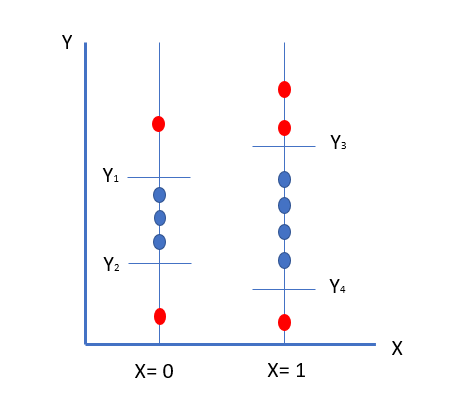
\includegraphics[width=0.50\columnwidth]{figures/chapter4_RuleExtraction/outlier_05.png}
  \end{tabular} 
  \caption{Rule extraction with a categorical variable.\label{fig:ch4-outlier5}}
\end{figure}

In that case, two rules would be extracted, one for each of the possible states of X:
\begin{itemize}
    \item Rule 1: NOT OUTLIER IF X = 0 $\land$ Y $\geq$ Y2 $\land$ Y $\leq$ Y1
    \item Rule 2: NOT OUTLIER IF X = 1 $\land$ Y $\geq$ Y4 $\land$ Y $\leq$ Y3
\end{itemize}

Generally speaking, the algorithm logic can be summarised as:
\begin{itemize}
    \item Apply OCSVM to the data set to create the model.
    \item Depending on the characteristics of variables, do:
    \begin{itemize}
    \item \underline{Case 1. Numerical only}:  Iteratively create clusters in the non-anomalous data (starting with one cluster) and create a hypercube using the centroid and the points further away from it. Check whether the hypercube contains any data point from the anomalous group; if it does, repeat using one more cluster than before. Finish when no anomalies are contained in the generated hypercubes. If there are anomalies and the data points in a cluster are inferior to the number of vertices needed for the hypercube, complete the missing vertices with artificial data points and finish when there are no anomalies or when the convergence criterion is reached.
    \item \underline{Case 2. Categorical only}: The rules will correspond directly to the different value states contained in the data set of non-anomalous points.
    \item \underline{Case 3. Both numerical and categorical}. This case would be analogous to Case 1, but data points will be filtered for each of the combinations of the categorical variables states. For each combination, there will be a set of rules for the numerical features.
    \end{itemize}
    \item Use these vertices to obtain the boundaries of that hypercube and directly extract rules from them.
\end{itemize}

Besides K-Means++, there are other clustering algorithms that may be applied. We will analyse also the rules obtained by applying K-Prototypes \parencite{ji2013improved}. The advantage of using K-Prototypes is that it can work directly with both categorical and numerical features.

The algorithms described within this section correspond to the two alternative methods within the \textbf{TC1 SVM+Prototypes reloaded} algorithm, which was introduced within \hyperref[sec:Hypotheses]{Section} \ref{sec:Hypotheses}.

\section{XAI metrics for rule extraction techniques}\label{sec:RuleExtractionMetrics}
In this section, we describe the different XAI metrics that we propose for assessing and comparing the quality of rule-based explanations. The metrics that we consider are divided into four subsets: \textit{comprehensibility}, \textit{representativeness}, \textit{stability} and \textit{diversity}. The reason behind it is that, to the best of our knowledge, some of these metrics do not have an algorithm implementation for the context of rule extraction techniques (they are only defined in a general way). This is the case of \textit{stability} and \textit{diversity}. The remaining metrics are chosen because they are relevant within the literature, and for the particular case of \textit{representativeness}, there are no frameworks that implement them within the context of P@k rules. 

We propose how to compute these metrics within this section, and we evaluate them over the case of unsupervised anomaly detection using OCSVM models. However, they could be applied for any model that has a binary output and that is explained through rule extraction techniques.

\begin{itemize}
    \item \textbf{Metrics for comprehensibility}: Number of rules ($nRules$), size of the rules ($sizeRules$).
    \item \textbf{Metrics for representativeness}: Percentage of data points explained with P@1 rules ($perP1$) and the median percentage coverage of data points by each rule ($p1Coverage$).
    \item  \textbf{Metrics for stability}: How many artificial points (similar to a subset of prototypes from the data set) are classified by the rules with the same predictions yielded by original blackbox model ($StabilityScore$).
    \item \textbf{Metrics for diversity}: Metric based on the degree of hyperspace overlapping between all the rules ($DiversityScore$).
\end{itemize}

\subsection{Metrics for comprehensibility}\label{subsec:RuleExtractionComprehensibility}
The metrics for \textit{comprehensibility} are directly analyzed from the rules themselves; $nRules$ is computed counting the number of rules generated, and $sizeRules$ is computed checking the elements that define the rule (i.e. $X > 3$ AND $X < 7$ AND $Y > 1$ have a $sizeRules=3$ while $X > 3$ have a $sizeRules=1$). This proposal already appears in \parencite{barakat2010rule}.

\subsection{Metrics for representativeness}\label{subsec:RuleExtractionRepresentativeness}
The metric $perP1$ for \textit{representativeness} simply checks the percentage of data points for the target class explained with P@1 rules. The other metric in this group is $p1Coverage$. It checks the median performance of the rules themselves: it computes the median percentage of coverage for the target class by each rule. These proposals are similar to \parencite{vilone2020comparative}, with the particularity of focusing on P@1 rules. We defined P@1 specifically, but it can be extended for other P@k thresholds.

\subsection{Metrics for stability}\label{subsec:RuleExtractionStability}
The metric $StabilityScore$ computes the \textit{stability} metric of the hypercubes. The first step is obtaining the prototypes from the data set and generate random samples near them. Then, obtain the prediction of the original model for those artificial samples and checks if the predictions using the rules are the same.

The steps for these metric are described below, and the detailed pseudocode appears in \hyperref[alg:ch4-stability]{Algorithm} \ref{alg:ch4-stability}. 

Model agreement:
\begin{itemize}
    \setlength{\itemindent}{2em}
    \item Choose N prototypes that represent the original hyperspace of data
    \item Generate M samples close to each of those N prototypes using Protodash algorithm \parencite{gurumoorthy2019efficient}; the hypothesis is that close points should be generally predicted belonging to the same class.
    \item For each of those N*M data points (M data points per each N prototype) check whether the rules (all of them) predict them as inliner or outlier; the data points that come into the function are either outliers or inliers. If they are inliers,  then the rules identify an artificial data point (of those M*N) as inlier if it is outside every rule. If the data points are outliers it's the same reversed: a data point is an inlier if no rule includes it.
    \item It then checks if the predictions using the rules for those artificial data points are the same as the one provided by the original model.
    \item With that, it computes \% of predictions for the artificial data points aforementioned that are the same between the rules and the original OCSVM model.
\end{itemize}

\hyperref[alg:ch4-stability]{Algorithm} \ref{alg:ch4-stability} receives the data set $X$ of inliers/outliers (depending if the rules are computed for inliers or outliers), the rules $X_r$ and the OCSVM fitted and trained model $clf$. Then obtains the protoypes with $ProtodashExplainer()$ function and generates the random samples $X_s$ near them with $randomNear()$, where an upper and lower limits ($th_s$, $th_l$) can be defined for how close are those points to the prototypes. Then, it checks which rules enclose that data point with $checkInR()$, and if at least one of them encloses the data point, it is considered that it can be classified using the rules. The metric $StabilityScore$ is specified in $n\_precision$ variable, that checks the percentage of agreement between the classifications using the rules and the ones with the model, through $checkInModel()$ function. 

\begin{algorithm}[h!]
\caption{StabilityScore}\label{alg:ch4-stability}
\begin{algorithmic}[1]
\Procedure{getAgreement}{$X, X_r, clf$}
    \State $X_p \gets ProtodashExplainer(X)$
    \State $X_s \gets []$
    \For{$p\in X_p$}
        \State $X_s \gets X_s.append(randomNear(p, th_l, th_s))$
    \EndFor\label{generate_samples}
    \State $n\_precision \gets 0$
    \State $l\_rules \gets []$
    \For{$d\in X_s$}
        \State $l\_iter \gets []$
        \For{$r\in X_r$}
             \State $l\_iter \gets l\_iter.append(checkInR(d, r))$
        \EndFor
        \State $r\_rules \gets max(l\_iter)$
        \State $r\_model \gets checkInModel(d, clf)$
        \If{$r\_rules = r\_model$}
            \State $n\_precision \gets n\_precision+1$
        \EndIf\label{compute_agreement}
       % \State $l\_rules \gets l\_rules.append(r\_rules)$
    \EndFor
    \State $n\_precision \gets n\_precision/len(X_s)$
    %\State $n\_agreement \gets l\_rules[=1]/len(X_s)$
    %\State \textbf{return} $n\_precision, n\_agreement$
    \State \textbf{return} $n\_precision$
\EndProcedure
\end{algorithmic}
\end{algorithm}

\hyperref[alg:ch4-stability]{Algorithm} \ref{alg:ch4-stability} corresponds to \textbf{TC2 StabilityScore}, which was introduced within \hyperref[sec:Hypotheses]{Section} \ref{sec:Hypotheses}.

Additionally, a proof that StabilityScore is a metric is included in \hyperref[sec:annex-demonstration-metric-stability]{Subsection} \ref{sec:annex-demonstration-metric-stability} within the \hyperref[ch:annex]{Annex}.

\subsection{Metrics for diversity}\label{subsec:RuleExtractionDiversity}
The metric to measure \textit{diversity} is $DiversityScore$, and it analyses if the rules are different with few overlapping concepts. This is computed checking the area of the hypercubes of the rules that overlaps with another one.
The way to check this is by seeing the 2D planes of each hypercube (by keeping two degrees of freedom for the features in the hyperplane coordinates; n-2 features are maintained and the other two are changed between their max/min values in order to obtain the vertices of that 2D plane). Then, it obtains the area of the 2D planes for the rules that overlaps, and each of those 2D areas is turned into a score between 0 and 1 by using the Jaccard similarity index and dividing the area of intersection of the 2D planes by their area of union.

The pseudocode for this metric appears in \hyperref[alg:ch4-score-intersect]{Algorithm} \ref{alg:ch4-score-intersect}. It receives the data set $X$ of inliers/outliers (depending if the rules are computed for inliers or outliers), the rules $X_r$, the list of columns for numerical features $l\_n$ and the one for categorical $l\_c$.
The first step is obtaining all the two tuples combinations of numerical features, using $combinations()$ function. After that, it obtains the combination of categorical values with function $unique()$. The algorithm then analyses separately the rules that belong to each categorical combination values. For each of those subset of rules $X\_r\_i$, if there are at least two rules, then it defines the tuples of possible rule combinations, $combR$. Then, it iterates per each combination of two numerical features. These two features will correspond to the features that will be changed, leaving the rest of the $l\_fix$ features fixed, in order to extract 2D planes from the hypercubes with $get2D$, and storing those planes in $polys$ variable. Those planes are used for obtaining the Jaccard similarity index with $scorePolys()$ function. If there is an iteration where one of the two dimensions has the same value, it is skipped since the area will be 0. ($checkEqual(pair_f)$).

\hyperref[fig:ch4-img-cubes]{Figure} \ref{fig:ch4-img-cubes} describes the process for an example in a 3D space. Since all the rules translate into a hypercube, we can choose two features at a time (leaving the rest fixed) and obtain the coordinates for those 2D planes (using their vertices values). Then, for two rules, we can see the area of overlapping between those 2D hyperplanes, as well as their area of union. With that areas, we obtain the Jaccard similarity index. Since the Jaccard similarity index ($score\_i$) yields a value between 0 and 1 (0 when there is no overlapping, and 1 when the area of intersection is the same as the area of union in a total overlapping), we can turn it into a metric in order to express a score value by doing $1-score\_i$, so a perfect score will be the one corresponding to no overlap between the rules. This is repeated for all 2D planes of the hypercubes, and we compute the mean of all the individual scores in order to have one final metric ($final\_score$) that is still between 0 and 1, with 1 the perfect score and 0 the worst.

\begin{figure}[h!]
\centering
  \begin{tabular}{c@{\qquad}c@{\qquad}c}
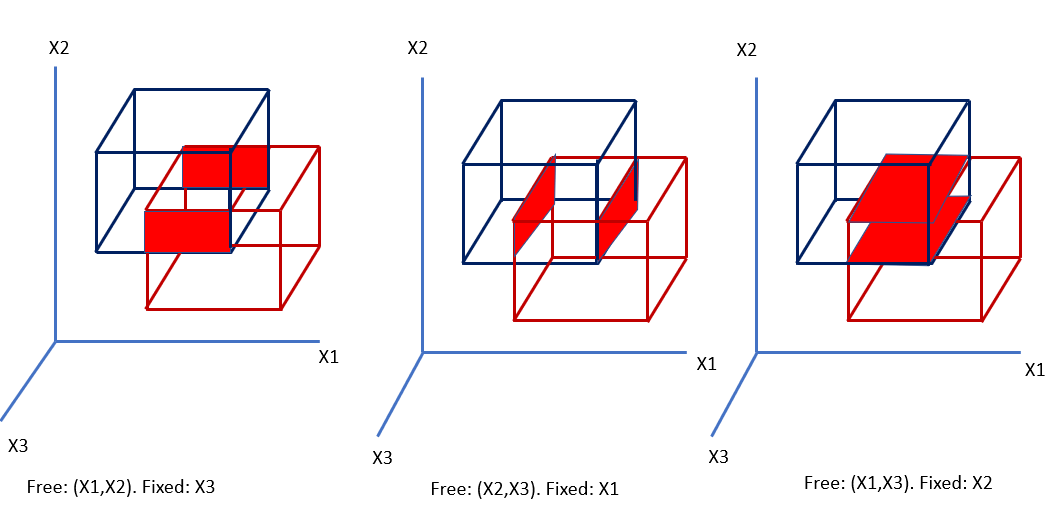
\includegraphics[width=0.8 \columnwidth]{figures/chapter4_RuleExtraction/img_cubes.png}
  \end{tabular} 
  \caption{The overlapping between rules (hypercubes) approximated using their 2D planes' area of intersection.\label{fig:ch4-img-cubes}}
\end{figure}

\begin{algorithm}[h!]
\caption{DiversityScore}\label{alg:ch4-score-intersect}
\begin{algorithmic}[1]
\Procedure{getInterScore}{$X, X\_r, l\_n, l\_c$}
    \State $l\_free \gets combinations(l\_n, 2)$
    \State $X\_c \gets unique(X[l\_c])$
    \State $score \gets []$
    \State $n\_inter \gets 0$
    \For{$cat \in rows(X\_c)$}
        \State $X\_r\_i \gets X\_r[cat]$
        \If{$len(X\_r\_i)>2$}
            \State $combR \gets combinations(X\_r\_i, 2)$
            \For{$pair_f \in l\_free$}
                \If{$checkEqual(pair_f)$}
                \State $continue$
                \EndIf
                \State $l\_fix \gets l\_n[!=pair_f]$
                \State $polys \gets get2D(combR, l\_fix,pair_f)$
                \State $score\_i, n\_i \gets scorePolys(polys)$
                \State $score \gets score.appends(1 - score\_i)$
                \State $n\_inter \gets n\_inter + n\_i$
            \EndFor
        \EndIf
    \EndFor
    \State $final\_score \gets mean(score)$
    \State \textbf{return} $final\_score$
\EndProcedure
\end{algorithmic}
\end{algorithm}

All the algorithms that we have proposed for computing XAI metrics are \textit{XAI-specific metrics}: metrics that are specific for a particular type of XAI technique (in this case, rule extraction).

\hyperref[alg:ch4-stability]{Algorithm} \ref{alg:ch4-stability} corresponds to \textbf{TC3 DiversityScore}, which was introduced within \hyperref[sec:Hypotheses]{Section} \ref{sec:Hypotheses}.

Additionally, a proof that DiversityScore is a metric is included in \hyperref[sec:annex-demonstration-metric-diversity]{Subsection} \ref{sec:annex-demonstration-metric-diversity} within the \hyperref[ch:annex]{Annex}.

\subsection{Towards one metric for summarizing all of them}\label{subsec:RuleExtractionOneMetric}
There is a question that will arise at this point: Which rule would be better? One with better results in \textit{comprehensibility}, or one with better results at, for instance, \textit{diversity}? When there is a need to choose a trade-off, which criteria should be prioritized? 
The answer to this will heavily depend upon the domain needs. However, in general terms, all the metrics can be combined into a single one that offers a unique view over them. It can be done with a metric in terms of $final\_metric = f(C, R, S, D)$ with C representing the comprehensibility metrics, R the representativeness, S the stability and D the diversity. There is another aspect that can be considered while creating a function to encapsulate all metrics. In general, it is better to have a lower value for comprehensibility metrics (less rules, less rule size) since that may contribute to an enhancement of comprehensibility. Regarding the rest of the metrics, higher values are better. Thus, a simple way to compute this is adding the results for representativeness, stability and diversity (adjusting their relative importance by a set of weights), and subtracting comprehensibility results. Since the values for the metric of comprehensibility are the only ones that are not in a range of 0 to 1, we scale them before computing this metric in order to have all values in the same range. This is done by dividing them with respect to the number of inliers or outliers (number of rules) or by a value based on the number of features (rule size).

With this, a higher final value will be better. This is expressed in \hyperref[eq:ch4-finalmetric]{Equation} \ref{eq:ch4-finalmetric}.

\begin{equation}\label{eq:ch4-finalmetric}
\begin{split}
  C = {\alpha_1 * (1 - nRules) + \alpha_2 * (1 - sizeRules)} \\
  R = \beta_1 * perP1 + \beta_2 * p1Coverage \\
  S = \gamma*StabilityScore \\
  D = \theta*DiversityScore \\
  final\_metric = \frac{(R + S + D + C)}{N} \\
\end{split}
\end{equation}
\myequations{Rule proposal: Final metric}

$N$ equals to the number of metrics considered (6 in this case). The different $\alpha$, $\beta$, $\gamma$ and $\theta$ parameters could be adjusted in order to weight the different metrics in case one of them is more important than others. Our proposed methods to compute a general metric is a very naive way to approach it, and more sophisticated ways could be explored. However, its important to highlight the need to be able to analyse everything together for some use cases, since there are many XAI aspects to measure and it may difficult to perform a comparison between XAI techniques.

\hyperref[eq:ch4-finalmetric]{Equation} \ref{eq:ch4-finalmetric} corresponds to \textbf{TC4}, which was introduced within \hyperref[sec:Hypotheses]{Section} \ref{sec:Hypotheses}.

\section{A framework for extracting and evaluating rule-based explanations}\label{sec:RuleExtractionFramework}
In this section, we describe our proposed general framework, \textbf{HyperRulEx} (\textbf{Hyper}cube \textbf{Rule} \textbf{Ex}traction), that standardizes rule extraction techniques, optimizes them, and obtains XAI specific metrics for assessing and comparing the quality of the explanations.

\subsection{Framework description}\label{subsec:RuleExtractionFramework}
The general flowchart followed by the framework appears in \hyperref[fig:ch4-flowchartRULEX]{Figure} \ref{fig:ch4-flowchartRULEX}. The first step applies a unsupervised ML algorithm for anomaly detection, yielding a binary output identifying the registers that are inliers and those that are outliers. Then, it applies a post-hoc rule extraction XAI algorithm that extracts the explanations. After that, the explanations are standardized by turning them into hypercubes, as exemplified in 
\hyperref[fig:ch4-format-not-homog]{Figure} \ref{fig:ch4-format-not-homog}. Then, after obtaining the hypercubes, the next step prunes the rules, eliminating those that are encapsulated by another bigger one. This step is described in more detail at \hyperref[subsec:RuleExtractionPruning]{Subsection} \ref{subsec:RuleExtractionPruning}. After that, it applies the XAI metrics \hyperref[sec:RuleExtractionMetrics]{Section} \ref{sec:RuleExtractionMetrics} for explanation evaluation. Even though our study focuses on XAI metrics that do not require a ground truth for the evaluation, the framework can be extended for including an evaluation against that ground truth both with specific XAI metrics as well as with model performance ones (e.g. F1).

\begin{figure}[h!]
\centering
  \begin{tabular}{c@{\qquad}c@{\qquad}c}
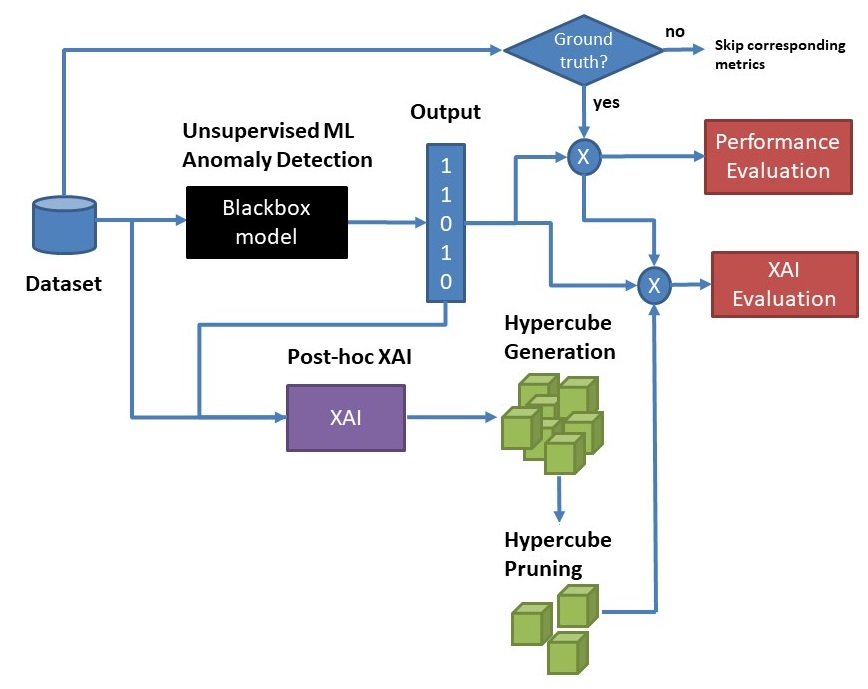
\includegraphics[width=0.80\columnwidth]{figures/chapter4_RuleExtraction/flowchartRULEX_notitle.jpg}
  \end{tabular} 
  \caption{Flowchart of the proposed framework that standardizes rule extraction XAI methods, optimizes the results and evaluate the final explanations with XAI  metrics.\label{fig:ch4-flowchartRULEX}}
\end{figure}


\begin{figure}[h!]
\centering
  \begin{tabular}{c@{\qquad}c@{\qquad}c}
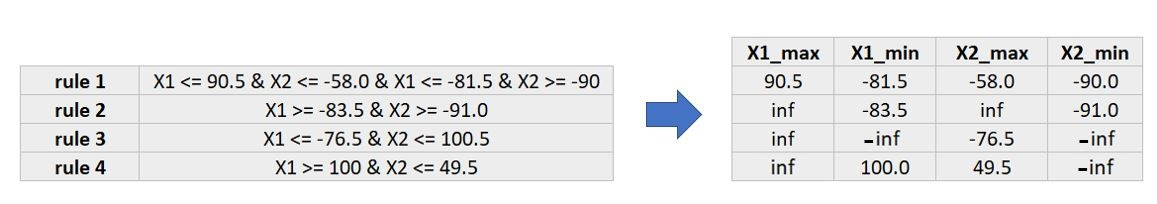
\includegraphics[width=0.95\columnwidth]{figures/chapter4_RuleExtraction/RuleFormatNotHomog4.JPG}
  \end{tabular} 
  \caption{Example showing the output of a rule extraction XAI algorithm over a sample case where there are only two input features. Left side shows the original rules yielded, where there are instances with redundant elements. Right side shows the hypercube (square in this case), corresponding to the transformed rules.\label{fig:ch4-format-not-homog}}
\end{figure}


\subsection{Pruning rules}\label{subsec:RuleExtractionPruning}
Many of the rules obtained with all the methods described above are suboptimal, since they can be enclosed into another bigger rule. In order to reduce the number of rules, and remove redundancies, we apply a simple pruning technique prior to the computing and evaluation of metrics.
We check every hypercube generated and see if their limits are inside any other rule. If they are, we eliminate that rule from the set of rules. We check this for every rule against every other rule in the data set, and we keep checking it in a loop until no rules are eliminated, until we reach a fixed point.

\section{Evaluation}\label{sec:RuleExtractionEvaluation}
This section presents the evaluation of hypothesis \textbf{H1} (described in \hyperref[sec:Hypotheses]{Section} \ref{sec:Hypotheses}) considering our proposal. The metric proposals described in \hyperref[sec:RuleExtractionMetrics]{Section} \ref{sec:RuleExtractionMetrics} serve directly as a justification for evaluating the hypothesis, since we provide a mathematical justification for these metrics. Nonetheless, we want to complement it by using our proposal over several data sets, applying the metrics for analysing the explanations obtained. With that, we want to show how the metrics are useful for finding out rule extraction techniques that are more suitable than others for a specific context (unsupervised anomaly detection with P@1 rules in this case), even if all those methods are post-hoc and model-agnostic. Because of that, we define several sub-hypotheses during this evaluation which serve as a reinforcement for checking \textbf{H1}.

In particular, we evaluate our proposal over data sets (both public and from Telefonica's real data), for assessing these following sub-hypotheses:
\begin{itemize}
    \item \textbf{Sub-hypothesis 1 (SH1):} The rule extraction method of \parencite{nunez2002rule} and our proposed variations applied over OCSVM for anomaly detection using a RBF kernel yield significantly less P@1 rules when applied for explaining inliers than for outliers or when using a linear kernel. \label{subhypothesis:subhypothesis4_1}
    \item \textbf{Sub-hypothesis 2 (SH2):} Our proposed variations over \parencite{nunez2002rule} yield similar results for P@1 rules that explain the inliers of an OCSVM anomaly detection model when compared to \parencite{nunez2002rule} in terms of explainability regardless of the kernel (considering Linear and RBF). \label{subhypothesis:subhypothesis4_2}
    \item \textbf{Sub-hypothesis 3 (SH3):} The rule extraction method of \parencite{nunez2002rule} and our proposed variations yield better results for P@1 rules that explain the inliers of an OCSVM anomaly detection model in terms of explainability than other rule extraction techniques and regardless of the kernel (considering Linear and RBF). \label{subhypothesis:subhypothesis4_3}
\end{itemize}

Explanations in terms of rule extraction for anomaly detection may help to see with a counterfactual view what would make an outlier turn into an inlier by explaining the inlier class (for local explanations). For explaining what feature values are normally associated with outlier data points (global explanations), these explanations will target the outlier class. This is why \textit{SH1} checks the contribution of RBF kernel for grouping data points inside its hypersphere in order to help explaining them with less rules.

For the hypothesis checks, we consider the results yielded by the XAI rule extraction methods over different data sets (\hyperref[subsec:RuleExtractionDataSets]{Section} \ref{subsec:RuleExtractionDataSets}), together with the type of kernel used for the OCSVM, as well as the type of data points explained (outliers or inliers). Thus, we have N data sets x 2 types of kernel x 2 types of data points. This serves for performing an hypothesis contrast based on the Wilcoxon signed-rank test \parencite{conover1998practical}, since it has been proved useful for comparing different ML model metrics results over several data sets for both classification \parencite{demvsar2006statistical} and regression tasks \parencite{trawinski2012nonparametric}.

The code is available for reproducibility through our published paper \parencite{barbado2022rule} or directly within the repository \parencite{Barbado2019}. The specific libraries and model configurations are detailed in \hyperref[sec:annex-rule-extraction-config]{Subsection} \ref{sec:annex-rule-extraction-config} within the \hyperref[ch:annex]{Annex} \ref{ch:annex}.

\subsection{Data sets}\label{subsec:RuleExtractionDataSets}
The data sets that we have used for evaluation belong to different domains, have different sizes and different number of features (both categorical and numerical), as indicated in \hyperref[table:ch4-rule-extraction-datasets]{Table} \ref{table:ch4-rule-extraction-datasets}:
\begin{itemize}
%    \setlength{\itemindent}{2em}
    \item Data sets 1 and 2 are about seismic activity \parencite{sathe2016lodes}. data set 1 is bi-dimensional with only numerical features ('gdenergy', 'gdpuls'). data set 2 has 2 categorical features ('hazard', 'shift') and 7 numerical ('seismoacoustic', 'shift', 'genergy', 'gplus', 'gdenergy', 'gdpuls', 'hazard', 'bumps', 'bumps2').
    \item Data set 3 is about cardiovascular diseases \parencite{padmanabhan2019physician}. There are 4 categorical features ('smoke', 'alco', 'active', 'is\textunderscore man') and 7 numerical ('age', 'height', 'weight', 'ap\textunderscore hi', 'ap\textunderscore lo','cholesterol','gluc').
    \item Data set 4 is from a call center at Telefónica (TEF Comms) \parencite{patent2019comms}. It is real data that includes the total number of calls received in one of its services during every hour. Using these data, some features are extracted (weekday), and they are cyclically transformed, so that each time feature turns into two features for the sine and cosine components. The rules in this case are also transformed back into the original features in order to enhance rule comprehension. 
    \item Data set 5 contains Telefónica's data about IoT devices attached to cars for vehicle tracking \parencite{patent2020fleet}. The data is aggregated in daily windows for each vehicle, representing features that model the daily behaviour of that vehicle. It contains 49 numerical features (such as the number of events with high RPM or the maximum temperature of the coolant), and 12 categorical ones (binary variables that indicate the model and make of that car, among others).
    \item Data set 6 refers to United States census for year 1990 \parencite{blake1998uci}. It has 2 categorical features ('dAncstry1\textunderscore 3', 'dAncstry1\textunderscore 4') and 7 numerical ones ('dAge', 'iYearsch', 'iFertil', 'iImmigr', 'iYearwrk', 'dTravtime', 'dRearning').
\end{itemize}

\begin{table}[h!]
\centering
\begin{tabular}{lllll} 
 \textbf{Data set} & \textbf{Ref.} & \textbf{Nº Cat.} & \textbf{Nº Num.} & \textbf{Nº Rows} \\ [0.5ex]
 \hline
 D1 & \parencite{sathe2016lodes} & 0 & 2 & 669\\ 
 D2 & \parencite{sathe2016lodes} & 2 & 7 & 1705\\
 D3 & \parencite{padmanabhan2019physician} & 4 & 7 & 42000\\
 D4 & \parencite{patent2019comms} & 0 & 5 & 2712\\
 D5 & \parencite{patent2020fleet} & 12 & 49 & 59844\\
 D6 & \parencite{blake1998uci} & 2 & 7 & 106819\\  [1ex]
\end{tabular}
\caption{Description of each data set, with their reference (Ref.), categorical features (Nº Cat.), numerical features (Nº Num) and number of rows.}
\label{table:ch4-rule-extraction-datasets}
\end{table}

\subsection{Results}\label{subsec:RuleExtractionResults}
In this subsection we describe the evaluation of our hypotheses. We will refer to K-Means approach as KM, and K-Prototypes as KP. Thus, for instance, K-Means with the "split" method will be identified as KM\_split.

% Hypothesis 1
\hyperref[table:annex-rule-extraction-hypothesis1]{Table} \ref{table:annex-rule-extraction-hypothesis1} provides the \textbf{results associated to \textit{\hyperref[subhypothesis:subhypothesis4_1]{SH1}}}. Here, we want to check if there are significantly less P@1 rules for inliers using a RBF kernel, compared to using a linear kernel for inliers, or the same RBF kernel for outliers. For the Wilcoxon signed-rank tests we only compare combinations of method-kernel-inliers/outliers for data sets that have at least 1 P@1 rule. Since the comparisons involve few data points in some cases, we check against a minimum p-value of 0.1. Considering this, only KM\_split and KM\_keep have significant differences in the number of rules. In those cases, H1 is actually rejected: RBF for inliers yields more rules than either RBF for outliers, or linear for inliers. Regarding the other methods, there are no statistically strong results to conclude anything. With that, even though it is not assured for every method, \textbf{these rule extraction methods when applied to inliers and when using a RBF kernel tend to generate more rules than in the other cases}.

% Hypothesis 2
After comparing those rule extraction methods in terms of the number of rules in order to see significant differences depending on the type of data points (inliers/outliers) and the type of kernel (RBF/linear), we proceed to check \textbf{\textit{\hyperref[subhypothesis:subhypothesis4_2]{SH2}}}. Here, we compare the methods considering all the XAI metrics proposed previously. This is done by checking every metric over every combination of data set, kernel and type of data (inliers/outliers), and performing a Wilcoxon signed-rank test in order to see if there are no significant differences between the methods for each of the metrics. Since the data points in this case are superior than those present at \textit{SH1}, we check against a minimum p-value of 0.05. For \textit{SH2}, there is no need to check the size of the rules since they will be the same for all the methods using K-Means and for all the methods using K-Prototypes. We only compare between data sets-kernel-type of data that exists in both methods considered. Thus, the means for the KM methods may vary depending on whether they are compared between them or they are compared against KP ones (and vice versa). 

At \hyperref[table:annex-rule-extraction-hypothesis1]{Table} \ref{table:annex-rule-extraction-xai-metrics-h2}, we see the methods and metrics that have significant differences according to Wilcoxon signed-rank test. There are some cases where the metrics do differ significantly, as some methods yield better results. \textbf{KM\_split method outperforms every other one regarding the percentage of data points covered by its P@1 rules (per\_p1). It does so in exchange of yielding a greater number of rules than some of the other methods, like KM\_keep\_reset}. Thus, it increases \textit{representativeness} by losing in terms of \textit{comprehensibility}. In general, KM methods cover more data points with P@1 rules that their counterparts with KP. Considering the other metric from \textit{representativeness}, p1\_coverage, there are no significant differences between KM\_split and KM\_keep\_reset, but both methods yield better results than KM\_keep. Thus, usually the P@1 rules that they yield are able to cover more data points. This is logical, since the algorithm that yields the rules in the case of KM\_keep tends to generate smaller hypercubes. An example of this can be seen in \hyperref[fig:ch4-evaluation-img-clustering-2D]{Figure} \ref{fig:ch4-evaluation-img-clustering-2D} for data set D1. We can see how KM\_keep indeed yields rules that are smaller than the ones from the other methods.  

\begin{figure}[h!]
\centering
  \begin{tabular}{c@{\qquad}c@{\qquad}c}
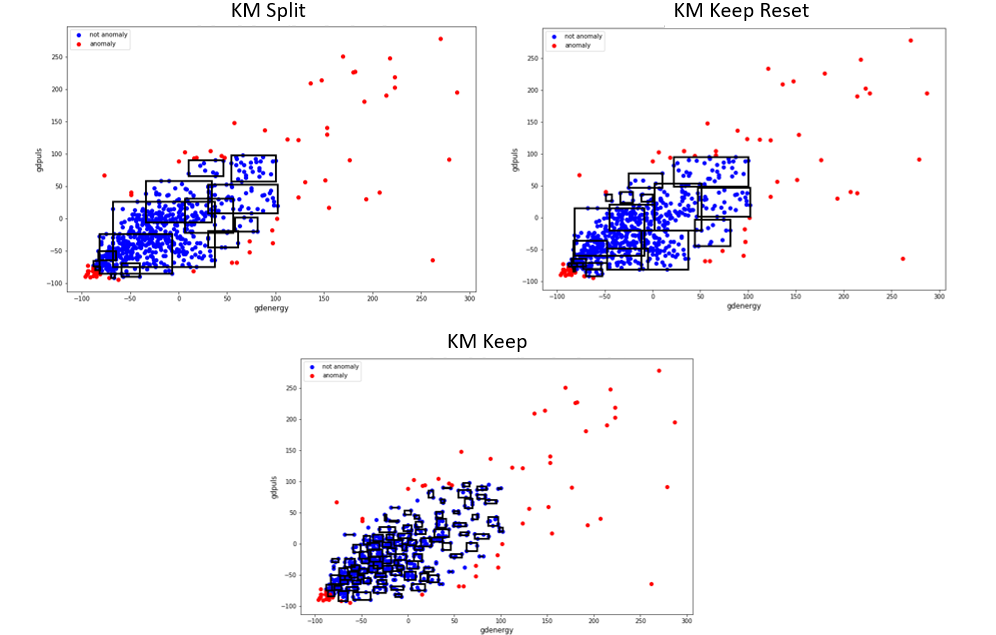
\includegraphics[width=0.9 \columnwidth]{figures/chapter4_RuleExtraction/clusteringMethods_comparison.PNG}
  \end{tabular} 
  \caption{K-Means based rule extraction methods (for inliers) over D1 data set with RBF kernel. \label{fig:ch4-evaluation-img-clustering-2D}}
\end{figure}

Regarding \textit{representativeness} (DiversityScore), there are no significant differences between KM methods, but all of them outperform all the KP ones. In terms of \textit{stability} (StabilityScore), we see no significant difference between any of the methods.
Finally, the general metric (final\_metric), shows that actually KM\_keep outperform KM\_split, and KM\_keep\_reset. Thus, even though KM\_keep had worse results in terms of \textit{representativeness} than the other KM methods, it is compensated by the other metrics.
With this analysis, we see that KM methods appear to be better than KP ones for P@1 rules and for explaining anomalies over a OCSVM model. However, KM methods are more contested; they seem to have similar results in some metrics (KM\_keep\_reset and KM\_discard are very similar between them), while being different in others (mainly compared to KM\_keep in terms of \textit{representativeness}). Thus, \textit{SH2} is partially supported. 

% Hypothesis 3
Finally, we check \textit{\hyperref[subhypothesis:subhypothesis4_3]{SH3}}. Since the techniques compared for \textit{SH2} yield similar results, we will only focus in KM\_split and KM\_keep, and benchmark them against the remaining rule extraction techniques covered in this chapter. \hyperref[fig:ch4-evaluation-img-other-2D]{Figure} \ref{fig:ch4-evaluation-img-other-2D} shows visualizations for some of these methods over D1 (when using a RBF kernel).

\begin{figure}[h!]
\centering
  \begin{tabular}{c@{\qquad}c@{\qquad}c}
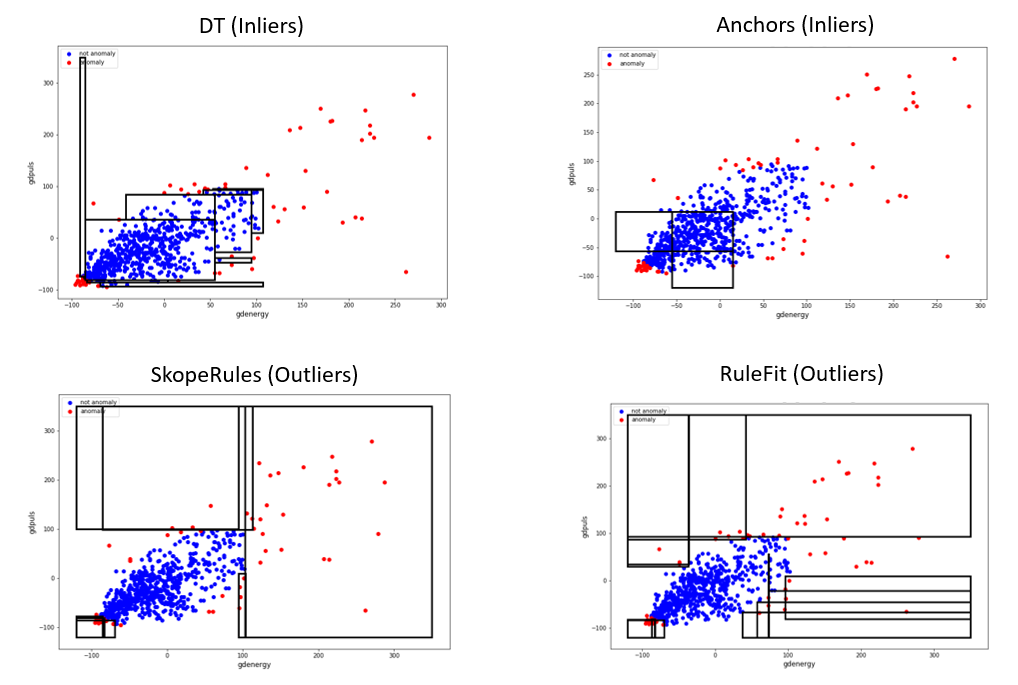
\includegraphics[width=0.9 \columnwidth]{figures/chapter4_RuleExtraction/RuleExtractionOther.PNG}
  \end{tabular} 
  \caption{Visualizations for the rules extracted over D1 with RBF kernel with DT and Anchors (for inliers) and SkopeRules and RuleFit (for outliers). \label{fig:ch4-evaluation-img-other-2D}}
\end{figure}


The results appear in \hyperref[table:annex-rule-extraction-xai-metrics-H3]{Table} \ref{table:annex-rule-extraction-xai-metrics-H3}. Here, we see how \textbf{KM\_split is generally better for every metric except for the ones related to \textit{comprehensibility}}. In particular, KM\_split is able to significantly cover more data points from the target class with P@1 rules (per\_p1) than any of the other methods, and also yields rules that have better coverage (p1\_coverage) than FRL and brlg. However, the mean coverage per rule compared to the other methods is not significantly different. Regarding \textit{stability}, KM\_split outperforms brlg, but brlg has a better result in terms of \textit{diversity}. KM\_split improves FRL and Anchors in \textit{stability}, and DT in \textit{diversity}. Finally, considering the general metric, KM\_split has significantly better results than any of the other methods, with the exception of DT, where it does not show significant differences. Considering KM\_keep, the results are similar, as shown in \hyperref[table:annex-rule-extraction-xai-metrics-H3-2]{Table} \ref{table:annex-rule-extraction-xai-metrics-H3-2}. One difference is that since KM\_keep has a better general metric than KM\_split, it is also able to significantly outperform DT in that aspect. Also, KM\_keep is not outperformed in terms of \textit{diversity} by brlg, as opposed to KM\_split.

As a conclusion, we see that both the solution of \parencite{nunez2002rule} with K-Means++ (and with the modification for generating rules for categorical features), together with the variations considered in this chapter (for also K-Means++ as clustering method) yield similar results in terms of most of the XAI metrics considered in this chapter for explaining the results of a OCSVM anomaly detection model using P@1 rules. The results in terms of \textit{comprehensibility} (number of rules) are influenced depending on the type of kernel used, and whether they are explaining inliers or outliers. Finally, comparing these techniques with other rule extraction methods, we saw a \textbf{trade-off between \textit{comprehensibility} and the remaining XAI metrics}. The clustering-based rule extraction techniques used in this chapter are able to explain better, using P@1 rules, the results of a OCSVM model (considering the data sets and kernels of this chapter) in terms of \textit{representativeness}, \textit{stability} and \textit{diversity}, but in exchange of \textit{comprehensibility}, which is penalized.


\section{Conclusion}\label{sec:RuleExtractionConclusion}
In this chapter, we presented variations over existing rule extraction XAI algorithms, as well as specific XAI metrics, for generating and evaluating explanations within the context of unsupervised ML for anomaly detection.
First, we highlighted that even though rule extraction XAI methods can theoretically be applied over unsupervised ML for anomaly detection (since the output is similar to that of a supervised binary classifier), there are specific considerations that should be taken into account, and there is a lack of research regarding that. Among these considerations, we find that there is commonly a great data imbalance between the two classes, there is normally a need to explain only one of the classes (outliers) in a counterfactual way, and the explanations must be P@1 within several use cases. Thus, some rule extraction techniques may be more suitable than others within this context. 
Because of that, we proposed \textbf{SVM+Prototypes reloaded}, an algorithm for generating both post-hoc global and local counterfactual rule-based explanations that are model agnostic.  This algorithm is a variant from a previous one within the literature, and comes with two alternative methods.
However, for evaluating and finding the best rule extraction technique in every context, we need quantitative metrics that measure the quality of the explanations against several aspects. Regarding this, we proposed several \textbf{XAI metrics} for measuring different aspects of the explanations generated. In particular, for measuring their \textit{comprehensibility, representativeness, stability and diversity}. For the particular cases of \textit{stability} and \textit{diversity}, we proposed novel metrics through \textbf{StabilityScore} and \textbf{DiversityScore} for measuring these aspects. We also discuss on the importance of combining all the metrics into one in order to simplify the analyses (although this is not necessary in some use cases).
Finally, we propose a framework that standardizes the output of the different rule extraction techniques in order to carry out the evaluation through those metrics. This framework also prunes the rules, eliminating redundant ones.
With that, we can consider our hypothesis \textbf{H1} (\hyperref[sec:Hypotheses]{Section} \ref{sec:Hypotheses}) validated by both mathematically justifying XAI metrics, as well as evaluating them over different data sets in order to quantify explanation differences between rule extraction methods within the context of unsupervised anomaly detection.
    \chapter{Explainable Anomaly Detection for Communications Data: Explanation Generation Using Prior Domain Knowledge Over OneClass SVM Models} \label{chap:5-comms-xai} 

In this chapter, we focus on the first of the two real use cases within this thesis for Explainable Artificial Intelligence (XAI) for real-world applications within the telecommunications industry. Specifically for this use case, the data feeds where anomalies need to be detected and explained is communications data, such as the number of received calls in a Call Center, or the data usage (e.g. bytes) of a cell phone across a time window.

We continue the analysis carried out in \hyperref[chap:4-rule-extraction]{Chapter} \ref{chap:4-rule-extraction}, but instead of working with a general XAI proposal, we evaluate its usage within a real-world context. A real-world context, like the one we are considering, has prior domain knowledge that can be included within the explanations. Our proposal in this chapter focuses on designing an XAI method for this specific use case, including a grid search variation that finds configurations for the anomaly detection method that yield explanations aligned to the prior knowledge. 

The contributions are related to \textbf{C2.1}, introduced in \hyperref[sec:Hypotheses]{Section} \ref{sec:Hypotheses} within the \hyperref[chap:3-objetives]{Chapter} \ref{chap:3-objetives}, and appear in our granted patent \parencite{patent2019comms}.

% Vincular este capitulo con el anterior, diciendo que pasamos a estudiar XAI en un caso de uso real donde se tiene que tener en cuenta ademas info a priori. Ademas, hablar de como en ocasiones como esta sirven soluciones más sencillas que un rule extraction general.


We divide this chapter in the following three sections. \hyperref[sec:ch5-IntroComms]{Section} \ref{sec:ch5-IntroComms} presents an introduction to the use case of LUCA Comms, including a description of the product and the specific XAI needs. \hyperref[sec:ch5-GeneralProposalComms]{Section} \ref{sec:ch5-GeneralProposalComms} describes our solution, \hyperref[sec:ch5-evaluation]{Section} \ref{sec:ch5-evaluation} presents an evaluation of our proposal, and, finally, \hyperref[sec:ch5-ConclusionComms]{Section} \ref{sec:ch5-ConclusionComms} summarizes main contributions presented in this chapter.

\section{Introduction}\label{sec:ch5-IntroComms}
This first section introduces the context of LUCA Comms, and details the need of using an XAI proposal along with an anomaly detection method for both predicting and explaining outliers within communications data. \hyperref[subsec:ch5-DescriptionComms]{Subsection} \ref{subsec:ch5-DescriptionComms} presents the use case of LUCA Comms, describing the type of data considered, as well as providing a brief introduction to the product itself. \hyperref[subsec:ch5-XAI-requirements-Comms]{Subsection} \ref{subsec:ch5-XAI-requirements-Comms} focuses on the XAI aspect for anomaly detection, describing the prerequisites that the XAI proposal should include in order to be aligned with the specific business needs.


\subsection{LUCA Comms description}\label{subsec:ch5-DescriptionComms}
LUCA Comms\footnote{The brand \textit{LUCA} has undertaken several changes due to business needs. Nonetheless, we will keep mentioning it within the product names for compliance with legacy documentations and references, in order to enhance clarity.} is a B2B (business to business) product, that receives data from the Movistar network\footnote{LUCA Comms is available in other countries, not only in Spain. In those cases, the data provider is another OB (Operating Business). However, for our analysis in this thesis, we focus on data from Spain only.} (21M mobile clients that generate 1 billion events per day) related to the usage of business lines from companies that have their communications contracted with Telefónica. These data serve as input to different analytical models that seek to extract useful insights for these companies, so that they obtain additional information about the usage that they are making of the communications services they have contracted. 

Among these analytical models and additional insights, LUCA Comms includes an anomaly detection module that provides information showing when there are anomalous patterns of the network usage for that particular company. This includes two approaches. 
First, LUCA Comms works with the mobile line usage from the employees of a company. Thus, a first context is providing information about the mobile lines from the company that have an anomalous behaviour related to other similar lines from the company and for the same type of mobile traffic. For instance, a company can detect if a mobile line from the sales department is having an anomalous outbound roaming traffic compared to other lines from the same department (sales) and for the same type of traffic (outbound roaming) on a specific day of week (e.g. Mondays).
Second, Luca Comms works with the calls received by the lines of a company (e.g. inside a Call Center). Because of that, another relevant need is detecting anomalies within the received calls, showing when there is an excessive number of calls (or the opposite). For instance, the Call Center of an insurance company can see whether the number of calls received on a particular day for a specific service (e.g. lines associated to hiring products) are normal or not (they are anomalies because the volume is too high or too low for that service in that particular date).

\hyperref[fig:ch5-comms-description]{Figure} \ref{fig:ch5-comms-description} shows a high-level schema of the product, where we see how data provided by the Telefónica network is combined with client specific data (e.g. the name of the Call Center service associated to several lines) for generating the insights within the product.

\begin{figure}[h!]
\centering
  \begin{tabular}{c@{\qquad}c@{\qquad}c}
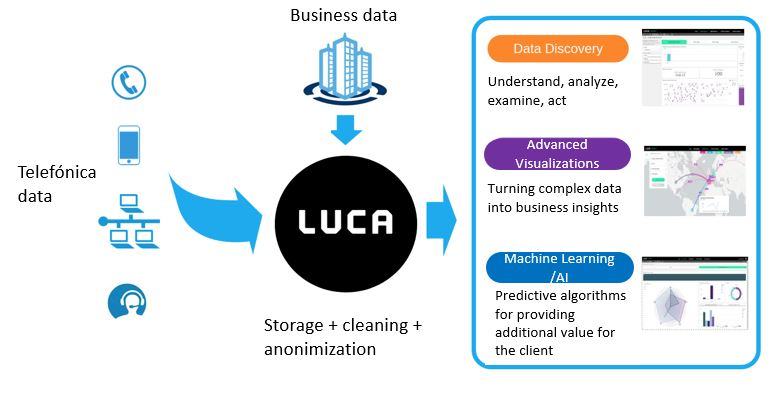
\includegraphics[width=0.90\columnwidth]{figures/chapter5_LucaComms/CommsDescription.JPG}
  \end{tabular} 
  \caption{Schema of LUCA Comms \parencite{patent2019comms}: It combines Telefónica's data with client specific data for generating the business insights within the product. \label{fig:ch5-comms-description}}
\end{figure}

Within these two anomaly detection needs, LUCA Comms is using a OneClass Support Vector Machine (OCSVM) algorithm for detecting data outliers. One of the reasons behind it is that OCSVM is an algorithm well-suited for detecting anomalies when using data sets that include temporal data \parencite{ma2003time}, as it is the case of LUCA Comms. However, deteting anomalies and providing a binary output is not enough, since customers want to know \textit{why} a specific data point is anomalous, and \textit{what} should have happened for it to be an inlier. This is why we needed to develop an Explainable AI (XAI) proposal that provides explanations that answer those questions, using as input the results from the OCSVM model.

\subsection{Specifications for explainability}\label{subsec:ch5-XAI-requirements-Comms}
As we already mentioned, LUCA Comms includes several OCSVM models, with a RBF (radial basis function) kernel, for predicting anomalies over different data sets. Nonetheless, all those data sets have in common one thing: there is only one numerical feature (e.g. bytes or number of calls), together with several categorical ones (e.g. day of week, if it is a holiday or not...). This characteristic of the data sets involved is an important detail that we will consider within our explainability approaches.
Along with this, the \textbf{business requirements} that should be met by the explanations are summarized as follows:
\begin{itemize}
    \item[\textbf{1.}] \textbf{Local explanations:} Explanations should justify why a specific data point is an anomaly.
    \item[\textbf{2.}] \textbf{Human-friendly:} Explanations should be easily understood by end-users of LUCA Comms. Thus, the features involved in the explanations must be comprehensible for them.
    \item[\textbf{3.}] \textbf{Counterfactual:} Explanations should indicate why a data point is an anomaly by indicating the changes that would turn the outlier into an inlier.
    \item[\textbf{4.}] The explanation generation method needs to be able to deal with \textbf{both numerical and categorical features}. %should show the counterfactual \textbf{changes in the numerical feature only}, within the context of specific combinations of categorical ones, However, it does not need to show counterfactual changes between categorical features.
\end{itemize}

%Without considering the underlying OCSVM ML model, those requirements could be met by a simple model such as a box-plot. Considering the subsets corresponding to each combination of categorical features, we could detect the anomalies through the box-plot whiskers. This is a whitebox model in itself, since the output shows directly in a visual way the numerical amount that should be changed in the numerical feature in order to turn an outlier into an inlier, for a specific combination of categorical features. However, there are two problems with this approach. 
%First, a box-plot will detect the anomalies for the subset of categorical combinations \textit{independently}, without considering the information of the other combinations. Thus, the anomalies in the number of received calls in a call center for a specific day of week and for a specific service will be obtained independently from the anomalies detected at that same service another day of the week, or independently from the anomalies detected in another service. 
%Second, using a box-plot approach will discard the OCSVM proposal, which was already validated for LUCA Comms. 
%With that, our goal is to obtain explanations that are \textit{similar} in structure to those of a box-plot, but by using the anomalies detected from an OCSVM model.

Without considering the underlying OCSVM ML model, those requirements could be met by a simple model such as a box-plot. Considering the subsets corresponding to each combination of categorical features, we could detect the anomalies through the box-plot whiskers. This is a whitebox model in itself, since the output shows directly in a visual way the numerical amount that should be changed in the numerical feature in order to turn an outlier into an inlier, for a specific combination of categorical features. However, there is a problem with this approach: a box-plot will detect the anomalies for the subset of categorical combinations \textit{independently}, without considering the information of the other combinations. Thus, the anomalies in the number of received calls in a call center for a specific day of week and for a specific service will be obtained independently from the anomalies detected at that same service another day of the week, or independently from the anomalies detected in another service. With that, our goal is to obtain explanations that are \textit{similar} in structure to those of a box-plot, but by using the anomalies detected from an OCSVM model.


\section{XAI proposal for explaining communications data}\label{sec:ch5-GeneralProposalComms}

In this section, we describe our proposal for predicting and explaining anomalies within communications data, within the use case of LUCA Comms.

The general process followed by LUCA Comms for detecting anomalies is detailed in \hyperref[fig:ch5-flowchart-comms]{Figure} \ref{fig:ch5-flowchart-comms}. First, using historical data, it finds the hyperparameters for the OCSVM through a grid search method that integrates prior domain knowledge in order to find hyperparameters combinations that yield results aligned with it. This step is described in \hyperref[subsec:ch5-HyperparamsComms]{Subsection} \ref{subsec:ch5-HyperparamsComms}. After that, it trains the OCSVM model with those hyperparameters, and applies our specific proposal for extracting the explanations, which includes a visual and counterfactual components. This is detailed in \hyperref[subsec:ch5-AnomalyLimitsComms]{Subsection} \ref{subsec:ch5-AnomalyLimitsComms}. Then, it both applies those limits to predict and explain the anomalies, both over the historical data used for training, as well as over new data that arrives in the system. New data can be included within the historical data when there is a need for model retraining. This is visualized through LUCA Comms application, as detailed in \hyperref[subsec:ch5-finalresult]{Subsection} \ref{subsec:ch5-finalresult}.

\begin{figure}[h!]
\centering
  \begin{tabular}{c@{\qquad}c@{\qquad}c}
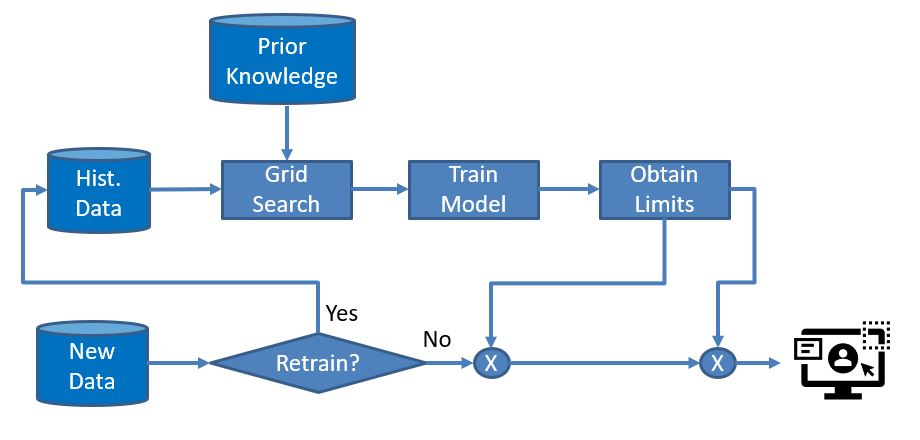
\includegraphics[width=0.80\columnwidth]{figures/chapter5_LucaComms/FlowChartComms.JPG}
  \end{tabular} 
  \caption{Flowchart describing the anomaly detection process of LUCA Comms \parencite{patent2019comms}\label{fig:ch5-flowchart-comms}}
\end{figure}


\subsection{Limit generation for visual and counterfactual explanations}\label{subsec:ch5-AnomalyLimitsComms}

In this subsection, we explain the method followed by our proposal for generating explanations over a blackbox OCSVM model for anomaly detection. As already mentioned in \hyperref[subsec:ch5-XAI-requirements-Comms]{Subsection} \ref{subsec:ch5-XAI-requirements-Comms}, the aim is to provide explanations from a OCSVM model that are visually similar to those of a box-plot, considering that there is only one numerical feature, and explaining the counterfactual changes that turn outliers into inliers within the isolated contexts of the different combinations of categorical values.

With that, the intuition behind our proposal is to first obtain the anomalies with the OCSVM, then filter the results for each combination of categorical values, and obtain the corresponding numerical value limit that differentiates inliers from outliers for each one of them, based on the information of the algorithm decision frontier. This is done by performing a \textbf{systematic random sampling} of values between the inliers and outliers for each categorical combination, and predicting their anomaly values with the ML model. Then, based on that information, we can infer the position of the decision frontier for that categorical combination. An example of the input and the output results is shown in \hyperref[fig:ch5-comms-limits-objective]{Figure} \ref{fig:ch5-comms-limits-objective}.

\begin{figure}[h!]
\centering
  \begin{tabular}{c@{\qquad}c@{\qquad}c}
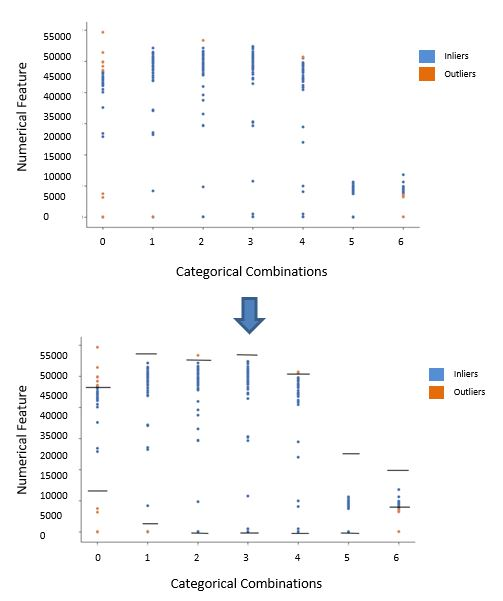
\includegraphics[width=0.70\columnwidth]{figures/chapter5_LucaComms/CommsLimits_Objective.JPG}
  \end{tabular} 
  \caption{Limit result: we aim to extract a reference value for the numerical feature and for each categorical feature combination by performing a systematic random sampling of values between them and predicting their values with the ML model. Y-axis represents the numerical variable, and X-axis a specific combination of categorical feature values \label{fig:ch5-comms-limits-objective}}
\end{figure}

The advantage of this approach is that we do not require the information of the position of the decision frontier by itself, thus providing a model-agnostic approach that could be applied over any black-box model, provided that the data set consists in one numerical feature and several categorical ones. 

The proposal for obtaining these limits for providing visual and counterfactual explanations corresponds to the contribution \textbf{TC6}, which was introduced within \hyperref[sec:Hypotheses]{Section} \ref{sec:Hypotheses}.

\hyperref[alg:ch5-ocsvm-comms-limits]{Algorithm} \ref{alg:ch5-ocsvm-comms-limits} describes in detail the process followed for generating the limits that will act as visual and counterfactual explanations over the results from the OCSVM model. It receives the input dataframe $X_i$, the numerical column name ($col\_name$), the list of categorical features ($l\_f$), the trained model, a constant for the number of random samples $N$, and coefficients for the upper/lower limits ($C_{sup}$ and $C_{inf}$ respectively). With that, it first gets the available combination of categorical columns with $unique(X_i[l_f])$. Then, it scales the data for the OCSVM model predictions and gets the anomaly predictions $X_a$. After that, it iterates through every categorical combination, and obtains the upper/lower inlier values for that subset of data. It also obtains the closest outliers to those inlier value references (the first outlier above the maximum inlier, and the first below the minimum inlier). If there are no outliers above/below within the dataset for that combination, the upper/lower reference is defined with an arbitrary offset over/under the upper/lower inliers. Then, we apply a \textbf{systematic random sampling} in order to obtain $N$ random points between the reference inlier and the reference outliers. Using those random samples, we obtain the model predictions, and we get the furthest random inliers to the upper/lower inliers. Those inliers will be the limits used for the explanations. In case all the random samples above/below are outliers, then the upper/lower inliers will be directly used as limits.

\hyperref[fig:ch5-anomaly-limit-example]{Figure} \ref{fig:ch5-anomaly-limit-example} serves as an example for the aforementioned algorithmic logic, where X-axis represents the categorical combinations and Y-axis the numerical feature. For category '0', since there are outliers above and below the inliers, the random sampling would be performed between them, in order to infer the anomaly limit (green line). For category '1', the same would be applied for the lower limit. However, since there are no outliers above the maximum inlier, the algorithm would first set an arbitrary high value and then perform the random sampling between that value and the highest outlier, yielding the limit after that. 


% Limit Generation
\begin{algorithm}[]
\caption{Limit generation for XAI over OCSVM}\label{alg:ch5-ocsvm-comms-limits}
\begin{algorithmic}[1]
\Procedure{generateLimits}{$X_{i}, col\_name, l_f, model, N, C_{sup}, C_{inf}$}

    % Get categorical combs
    \State $d_{comb} \gets unique(X_i[l_f])$
    
    % Data Preparation
    \State $X, scaler \gets scaling(X, l_f)$
    
    % Get predictions
    \State $X_{a} \gets scaler.unscale(model.predict(X, scaler))$ 
    
    % Store results
    \State $d\_limits \gets dict()$
    
    % Iter per categ. comb 
    \For{$comb \in d_{comb}$}
        % Iter params & min/max inliers
        \State $X\_iter \gets X_{a}[l_f = comb]$
        \State $X_{in} \gets X_{a}[anomalies = False]$ 
        \State $X_{out} \gets X_{a}[anomalies = True]$ 
        \State $min_{in}, max_{in} \gets MinMax(X_{in}[col\_name])$
        \State $ref\_above_{out} \gets min(X_{out}[col\_name] \geq max_{in})$
        \If{$len(ref\_above_{out}) = 0$}
            \State $ref\_above_{out} \gets C_{sup} \times max_{in}$
        \EndIf
        \State $ref\_below_{out} \gets max(X_{out}[col\_name] \leq min_{in})$
        \If{$len(ref\_below_{out}) = 0$}
            \State $ref\_below_{out} \gets C_{inf} \times min_{in}$
        \EndIf
        
        % Get random sampling
        \State $X_{above} \gets randomSample(max_{in}, ref\_above_{out}, l_f, N)$
        \State $X_{below} \gets randomSample(min_{in}, ref\_below_{out}, l_f, N)$
        \State
        % Get predictions & keep outliers only
        \State $X_{above} \gets model.predict(scaler.scale(X_{above}))$
        \State $X_{above} \gets scaler.unscale(X_{above})$
        \State $X_{above} \gets X_{above}[anomalies = False]$
        \State $X_{below} \gets model.predict(scaler.scale(X_{below}))$
        \State $X_{below} \gets scaler.unscale(X_{below})$
        \State $X_{below} \gets X_{below}[anomalies = False]$
        \State
        % Inliers above & below
        \If{$len(X_{above}) > 0$ $\&$ $len(X_{below})>0$} 
            % Keep as reference the upper random inlier
            \State $lim_{sup} \gets max(sort(X_{above}[col\_name], asc=False))$
            \State $lim_{inf} \gets min(sort(X_{below}[col\_name], asc=False))$
        
        % All points above are outliers
        \ElsIf{$len(X_{above}) > 0$ $\&$ $len(X_{below})=0$} 
            % Keep as reference directly the upper inlier
            \State $lim_{sup} \gets max_{in}$
            \State $lim_{inf} \gets min(sort(X_{below}[col\_name], asc=False))$
        
        % All points below are outliers
        \ElsIf{$len(X_{above}) = 0$ $\&$ $len(X_{below})>0$} 
            % Keep as reference directly the lower inlier
            \State $lim_{sup} \gets max(sort(X_{above}[col\_name], asc=False))$
            \State $lim_{inf} \gets min_{in}$
        
        % All anomalies
        \Else
            % Keep as reference directly the upper/lower inliers
            \State $lim_{sup} \gets max_{in}$
            \State $lim_{inf} \gets min_{in}$
        
        \EndIf
        
    \State $d\_limits[comb][lim_{sup}] \gets lim_{sup}$
    \State $d\_limits[comb][lim_{inf}] \gets lim_{inf}$
    \EndFor

\State \textbf{return} $d\_limits$

\EndProcedure
\end{algorithmic}
\end{algorithm}

\begin{figure}[h!]
\centering
  \begin{tabular}{c@{\qquad}c@{\qquad}c}
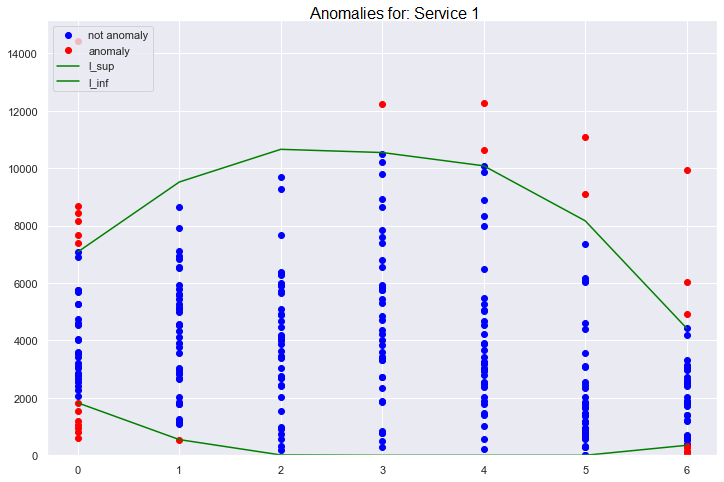
\includegraphics[width=0.70\columnwidth]{figures/chapter5_LucaComms/AnomalyLimits_example.png}
  \end{tabular} 
  \caption{An example of the anomaly limit generation, where the logic depends on whether there are anomalies above/below the inliers for each category or not. \label{fig:ch5-anomaly-limit-example}}
\end{figure}


\subsection{Hyperparameter search}\label{subsec:ch5-HyperparamsComms}

The method for obtaining the limits, described in \hyperref[subsec:ch5-AnomalyLimitsComms]{Subsection} \ref{subsec:ch5-AnomalyLimitsComms} is only suitable for when there are no outliers in the middle of the inliers. This is shown in \hyperref[fig:ch5-anomaly-limit-problem]{Figure} \ref{fig:ch5-anomaly-limit-problem}, where there are outliers between the inliers. This is something that may appear within the context we are working with, since an OSCVM that uses a RBF kernel may have more than one \textit{landmark}. When that is the case, there may be more than one upper and one lower limit that separates inliers from outliers per each categorical value combination. 

\begin{figure}[h!]
\centering
  \begin{tabular}{c@{\qquad}c@{\qquad}c}
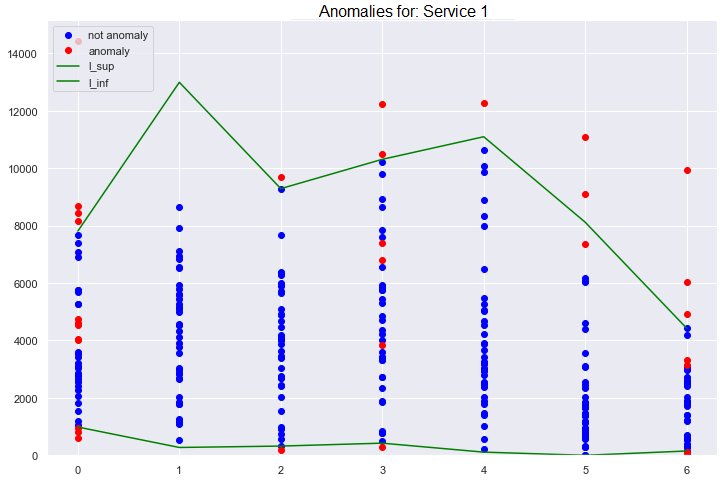
\includegraphics[width=0.70\columnwidth]{figures/chapter5_LucaComms/AnomalyLimits_example_problem.png}
  \end{tabular} 
  \caption{Inferring the limits based on the random sampling proposal already mentioned is not suitable for when there are anomalies within the inliers. \label{fig:ch5-anomaly-limit-problem}}
\end{figure}

This problem highlights an additional business need: the explanations should only show outliers above/below the inliers. It would not be helpful to indicate, for instance, that an amount of received calls in a particular call center service is \textit{not anomalous} if it is between a range of values or between another range of values, but in the middle of those ranges, the values are anomalous. This can be seen, for instance, at the categorical combination of 0 in \hyperref[fig:ch5-anomaly-limit-problem]{Figure} \ref{fig:ch5-anomaly-limit-problem}. The explanations should consider a \textbf{prior domain knowledge}: anomalies should only be above or below the inliers, but not between them. In this case, this prior domain knowledge is in fact a \textbf{rule} that should be taken into account during the explanation generation process. 

Following the taxonomy of \parencite{beckh2021explainable}, which covers different approaches for integrating prior knowledge in the explanation generation, we need an approach within the context of \textbf{Informed Machine Learning}\footnote{It is important to note that the article \parencite{beckh2021explainable} was developed after our proposal. Thus, we did not have this taxonomy at the beginning for guiding our research. Nonetheless, our proposal falls inside the aforementioned category.}. This is because we are not using a post-hoc model for building the explanations. Instead, we are obtaining them directly from the information of the model (the decision frontier). Thus, the prior knowledge needs to be included at the ML model level. 
Our proposal to include this knowledge is placed within the \textbf{hypothesis set} type of knowledge integration. In particular, we aim to include that knowledge within the hyperparameter grid search, in order to choose the best parameter configuration that is also aligned with that business rule.

OCSVM has two important hyperparameters to optimize:
\begin{itemize}
    \item $\gamma$: It is the \textit{rejection rate}, which defines the maximum limit for the fraction of points that could be considered an anomaly.
    \item $\nu$: It is the fraction for the limit of the number of support vectors. This limits the number of support vectors used, defining the minimum limit for the fraction of points that could be used as support vectors.
\end{itemize}

Those parameters lead to the following trade off \parencite{xiao2014parameter}:
\begin{itemize}
    \item \textit{Decrease the rejection rate}: \textit{increases} the space for non-anomalous points; fewer anomalies detected. This may lead to overfitting.
    \item \textit{Increase the rejection rate}: \textit{decreases} the space for non-anomalous points; more anomalies detected. this may lead to underfitting.
\end{itemize}
Even though the previous points define the trade off for $\gamma$, the problem is similar with $\nu$.

However, OCSVM is used as an unsupervised ML algorithm, which means that the hyperparameter optimization, and its combination with prior domain knowledge, should also be done in an unsupervised manner.

The MIES (\textit{measure the distance from samples to enclosing surfaces}) algorithm \parencite{xiao2014parameter} proposes an approach for computing a score that can be used for finding the best hyperparameter configuration. It proposes a way to perform a grid search for OCSVM as long as the kernel used is RBF (which is the one that we are already using within our approach). The method calculates the normalized distance (ND) of the data (target data) to the decision frontier, for both data points outside the decision boundary (edge patterns, EP), and within it (interior patterns, IP), and with that information it decides which combination of hyperparameters is optimal.
To do that, it first calculates the ND for the IPs. The IPs should be as far away as possible from the decision frontier. This will avoid underfitting (too many anomalies detected), since the obtained decision frontier will not be too close to the inliers. Because of this, the optimal choice would be the one that maximizes this criterion. But that criterion alone is not enough because it will lead to overfitting due to the large non-anomalous space that would be generated (and fewer anomalies would be detected). Therefore, another criterion to consider is the ND for EP. They should be as close as possible to the decision frontier. That way, that decision frontier would respect and better capture the distribution of the underlying data. This is summarized in \hyperref[fig:ch5-mies-example]{Figure} \ref{fig:ch5-mies-example}.

\begin{figure}[h!]
\centering
  \begin{tabular}{c@{\qquad}c@{\qquad}c}
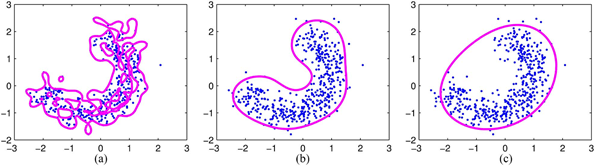
\includegraphics[width=0.90\columnwidth]{figures/chapter5_LucaComms/MIES_examples.png}
  \end{tabular} 
  \caption{Some examples of decision frontiers obtained for different use cases \parencite{xiao2014parameter}. Example (c) shows a decision frontier obtained by trying only to maximize the distance from the interior points (IPs) to the decision frontier. Example (a) shows a decision frontier obtained only by trying to minimize the distance from the edge points (EPs) to the decision frontier. The optimal situation is (b) where both factors are taken into account. \label{fig:ch5-mies-example}}
\end{figure}

With that, the objective function from MIES is the following one:
$fo(s) = max ND(x_i) - max ND(x_j)$
With $x_i$ the IP, $x_j$ the EP, and ND the normalized distance. The $max$ function returns the maximum distance value among all the data points for each of those two groups, IP and EP. 
The normalized distance is obtained as follows:
$ND = frac{d}{1 - d_{\pi}}$ 
With $d$ the distance of each data point to the decision frontier, and $d_{\pi}$ a reference distance computed between the origin of coordinates (OO) and an hyperplane obtained from the decision frontier.

Using that hyperparameter selection as a reference, we propose an algorithm that first filters out hyperparameter configuration that do not comply with the prior domain knowledge, and then applies MIES algorithm in order to find the best one of them. \hyperref[alg:ch5-ocsvm-comms-gridsearch]{Algorithm} \ref{alg:ch5-ocsvm-comms-gridsearch} describes the process followed. It receives the input dataframe $X_i$, the numerical column name ($col\_name$), the list of categorical features ($l\_f$), and a dictionary $dct_{hyper}$ with the different hyperparameter ranges for $\nu$ and $\gamma$. With that, it first gets the available combination of categorical columns with $unique(X_i[l_f])$. Then, it scales the data for the OCSVM model training and the MIES score. After that, it initializes a dictionary with the results (hyperparameter values and metric scoring) $d\_ref$. Following this, it iterates through the different hyperparameters, and gets the corresponding model predictions with $fitPredict(X, scaler)$. The values in $X_a$ are unscaled. Before computing the MIES metric, the algorithms checks that no outliers are between the inliers for each categorical combination. If at least one categorical combination has outliers between the inliers, that hyperparameter configuration is skipped. When there are no outliers between the inliers, the algorithm proceeds to obtain the MIES metric score ($MIES(X, scaler, l_s)$), and when that score improves the score from the previous iteration, it keeps it as the best reference. 
The algorithm finally returns the MIES score, along with the corresponding $\nu$ and $\gamma$ for that best hyperparameter configuration.

% MIES Variation
\begin{algorithm}[]
\caption{Grid search with prior knowledge along with MIES}\label{alg:ch5-ocsvm-comms-gridsearch}
\begin{algorithmic}[1]
\Procedure{gridSearch}{$X_{i}, col\_name, l_f, dct_{hyper}$}

    % Get categorical combs
    \State $d_{comb} \gets unique(X_i[l_f])$
    
    % Data Preparation
    \State $X, scaler \gets scaling(X, l_f)$
    
    % Default reference
    \State $d\_ref \gets dict()$
    \State $d\_ref[score] \gets -\infty$
    \State $d\_ref[\nu] \gets null$
    \State $d\_ref[\gamma] \gets null$
    
    % Iter per hyperparameter combinations
    \For{$params \in dct_{hyper}$}
    
        % Init params
        \State $d\_iter \gets dict()$
        \State $d\_iter[\nu, \gamma] \gets params[\nu, \gamma]$
        \State $flagInside \gets False$
        
        % Get predictions
        \State $X_{a} \gets scaler.unscale(fitPredict(X, scaler))$ 
        
        % Iter per categ. comb and check middle points
        \For{$comb \in d_{comb}$}
            \State $X\_iter \gets X_{a}[l_f = comb]$
            \State $min_L, max_L \gets MinMax(X\_iter[anomalies = 0][col\_name])$
            \State $X_{check} \gets X\_iter[anomalies = 1$ \& $col\_name \geq min_L$ \& $col\_name \leq max_L]$
            \If{$len(X_{check})$} 
                \State $flagInside \gets True$
            \EndIf
        \EndFor
        
        \If{$flagInside = True$}
            \State $continue$
        \EndIf
        
        % Get MIES metric if there are no middle points
        \State $dct\_results \gets MIES(X, scaler, l_s)$
        
        % Keep result as reference if better than previous
        \If{$dct\_results[score] \geq d\_ref[score]$}
            \State $d\_ref[score] \gets dct\_results[score]$
            \State $d\_ref[\nu] \gets dct\_results[\nu]$
            \State $d\_ref[\gamma] \gets dct\_results[\gamma]$
        \EndIf
        
    \EndFor
        
    \State \textbf{return} $d\_ref$
    
\EndProcedure
\end{algorithmic}
\end{algorithm}


\hyperref[alg:ch5-ocsvm-comms-gridsearch]{Algorithm} \ref{alg:ch5-ocsvm-comms-gridsearch} corresponds to the contribution \textbf{TC7}, which was introduced within \hyperref[sec:Hypotheses]{Section} \ref{sec:Hypotheses}.

\pagebreak

\subsection{Final result}\label{subsec:ch5-finalresult}


% Hablar de como se aplican las franjas que se calculan por comb de categoricas sobre cada dia luego para ver si hay o no anomalías (es decir, explicar cual es la visualizacion final, y luego vincularlo con el ejemplo del dashboard final donde se filtra por servicios)

After having the upper and lower limits of each numerical variable with respect to the different combinations of categorical ones, those limits are used for both explaining the already detected anomalies within the historical data, as well as for predicting new anomalies, as shown in \hyperref[fig:ch5-comms-anomalies-viz]{Figure} \ref{fig:ch5-comms-anomalies-viz}. There, we see how the visualization shows one plot per categorical combination for all categorical variables that are not daily-related, and then, since the X-axis includes the different dates, the limits on that day will correspond to the categorical combinations of the daily-related for that specific date (week day in our case, but there can be others, like if it is a holiday or not).

\begin{figure}[h!]
\centering
  \begin{tabular}{c@{\qquad}c@{\qquad}c}
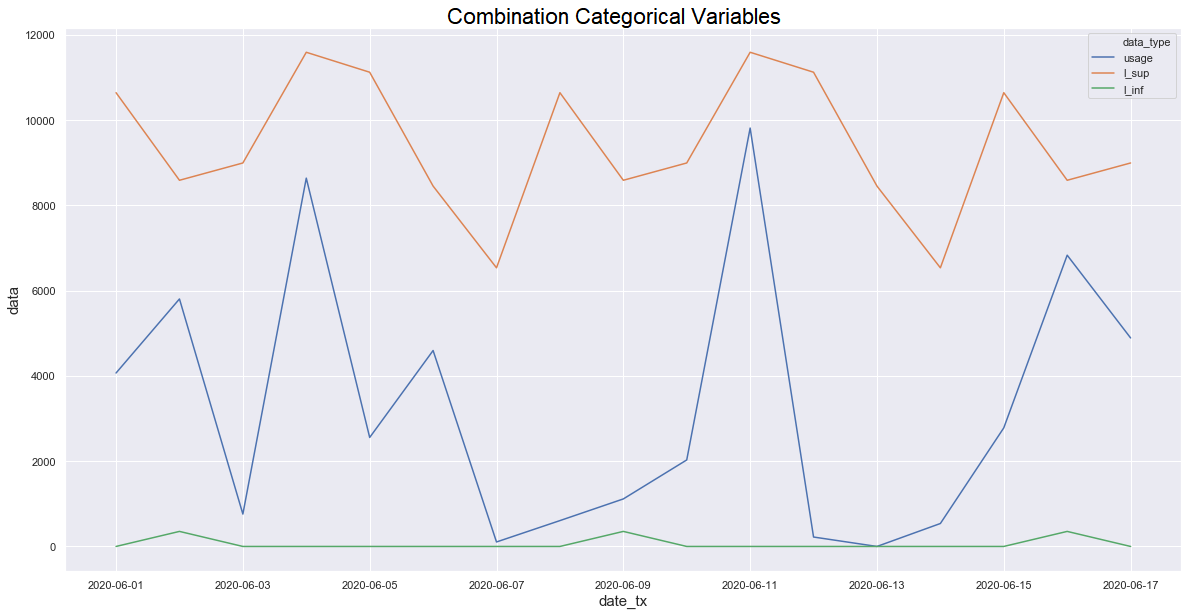
\includegraphics[width=0.9\columnwidth]{figures/chapter5_LucaComms/ThresholdsResults.png}
  \end{tabular} 
  \caption{Example of the applications of the limits over the historical data evolution \label{fig:ch5-comms-anomalies-viz}}
\end{figure}

The final visualization within LUCA Comms is shown in \hyperref[fig:ch5-comms-anomalies-result]{Figure} \ref{fig:ch5-comms-anomalies-result}. Users first select a filter for the categorical variables on the left (in our case, service name for CC or combination of organizational levels for M), the numerical variable, and then they see the data evolution for a specific period of time, with the corresponding limits, and highlighting the dates that are anomalous. Hovering over that date, they can see the counterfactual explanation, showing the actual value and the value that it should be for that date in order to be an inlier.

\begin{figure}[h!]
\centering
  \begin{tabular}{c@{\qquad}c@{\qquad}c}
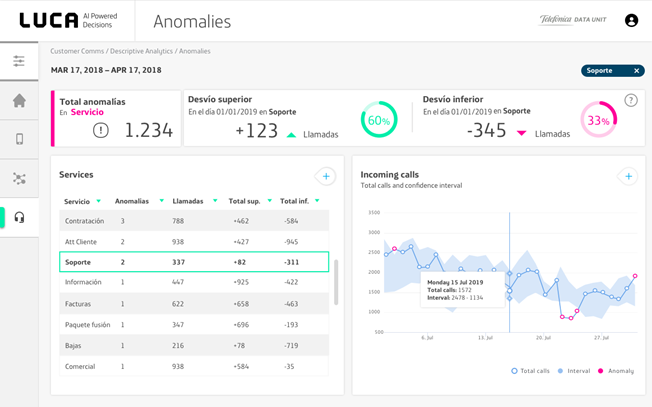
\includegraphics[width=0.9\columnwidth]{figures/chapter5_LucaComms/CommsAnomalies.png}
  \end{tabular} 
  \caption{Example of the XAI approach for anomaly detection within LUCA Comms product. \label{fig:ch5-comms-anomalies-result}}
\end{figure}

\section{Evaluation}\label{sec:ch5-evaluation}
In this section, we highlight some aspects regarding the evaluations carried out. First, we describe the datasets that we have used in \hyperref[subsec:ch5-DataComms]{Subsection} \ref{subsec:ch5-DataComms}, and then we focus on the evaluations themselves along with the hypothesis checked, in \hyperref[subsec:ch5-ResultsComms]{Subsection} \ref{subsec:ch5-ResultsComms}.

Our aim is to use this analysis for evaluating \textbf{H2}, described in \hyperref[chap:3-objetives]{Chapter} \ref{chap:3-objetives} at
\hyperref[sec:Hypotheses]{Section} \ref{sec:Hypotheses}, within the context of communications data. The reason behind it is that here, we are considering prior domain knowledge along with XAI for anomaly detection, including it for adjusting the explanations generated. Thus, we aim to check how this can indeed be done using real-world data, as well as showing how this is compatible with not having a significant decrease in the predictive power of the anomaly detection algorithm.

\subsection{Data involved}\label{subsec:ch5-DataComms}
In this subsection, we describe the data sets used for the initial validations of our proposal. We use two types of data sets, one for the usage of customer's mobile lines (M), and other regarding the received calls in lines associated to customer's services (e.g. Call Center lines, CC). The two types of data sets have in common that there is only one numerical variable, together with several categorical ones.

% Variables M y qué representan, qué variables se usan para anomalías y cómo se preprocesan
Regarding the data set for M, there are five different numerical variables that will be considered along with the categorical ones. Since we are dealing with an univariate approach regarding the numerical variable, we work with five different data sets, explaining the anomalies in each one of those variables independently, within the context of the categorical ones. Below, we indicate the different numerical variables used:

\begin{itemize}
    \item \textbf{National voice}: Minutes of voice for national calls.
    \item \textbf{Roaming out voice}: Minutes of voice for roaming out calls.
    \item \textbf{National data}: Bytes used in data traffic for national web navigation.
    \item \textbf{International voice}: Minutes of voice for international calls
    \item \textbf{Roaming data}: Bytes used in data traffic for roaming data.
\end{itemize}

For M, the categorical variables that are included as a context for the initial validations are:

\begin{itemize}
    \item \textbf{Weekday}: Day of the week associated to the traffic type.
    \item \textbf{Organizational level 2}: A organization which encloses several mobiles lines (e.g. \textit{People Analytics} department)
    \item \textbf{Organizational level 1}: A hierarchical organizational level from a company, that references the parental organization from \textbf{Organizational level 2} (e.g. \textit{Human Resources} to \textit{People Analytics} department)
\end{itemize}

% Distribucion datos M
\hyperref[table:ch5-mf-distribution]{Table} \ref{table:ch5-mf-distribution} describes the different data sets used for the validations with M, using the information of three clients. 

\begin{table}[h!]
\centering
\resizebox{0.8\textwidth}{!}{%
\begin{tabular}{@{}lllllll@{}}
\toprule
\textbf{Client} & \textbf{N Size} & \textbf{Min Date} & \textbf{Max Date} & \textbf{N Lines} & \textbf{N Org Level 1} & \textbf{N Org Level 2} \\ \midrule
C1  & 1120766 & 2019-11-08 & 2020-06-17 & 7808  & 30 & 32 \\
C2  & 3031749 & 2020-03-09 & 2020-08-31 & 20936 & 1  & 1  \\
C3      & 145398  & 2019-08-17 & 2020-06-17 & 995   & 6  & 19 \\ \bottomrule
\end{tabular}%
}
\caption{Data distribution for M, which includes the data set size, the period range considered, and the different organizational levels. C2 organizational information was not available; thus, there is a generic organization that encloses all the lines.}
\label{table:ch5-mf-distribution}
\end{table}

% Variables CC y qué representan, qué variables se usan para anomalías y cómo se preprocesan
For CC, there is only one numerical feature (number of calls), along with the categorical ones. They are described below:
\begin{itemize}
    \item \textbf{Number of calls}: Total number of calls received in a particular day for a specific service. It sums all the calls received by the lines associated to that service.
    \item \textbf{Weekday}: Day of the week associated to the daily received calls.
    \item \textbf{Service}: Service associated to several specific lines (e.g. 'Customer Support' service)
\end{itemize}

% Distribucion datos CC
\hyperref[table:ch5-cc-distribution]{Table} \ref{table:ch5-cc-distribution} describes the different data sets used for the validations with CC, using the information of three clients. 
\begin{table}[h!]
\centering
\resizebox{0.6\textwidth}{!}{%
\begin{tabular}{@{}llllll@{}}
\toprule
\textbf{Client} & \textbf{N Size} & \textbf{Min Date} & \textbf{Max Date} & \textbf{N Lines} & \textbf{N Services} \\ \midrule
C1  & 4632   & 2019-11-16 & 2020-06-17 & 52   & 47   \\
C4       & 12222  & 2019-07-04 & 2020-06-17 & 47   & 19   \\
C2 & 214590 & 2020-03-09 & 2020-08-31 & 1727 & 1727 \\ \bottomrule
\end{tabular}%
}
\caption{Data distribution for CC, which includes the data set size, the period range considered, and the different services.}
\label{table:ch5-cc-distribution}
\end{table}

Finally, in \hyperref[table:ch5-ground-truth]{Table} \ref{table:ch5-ground-truth} we see the ground truth available per client, data set and numerical variable, which includes the total data points within it along with the total daily anomalies\footnote{
Not all the data sets from \hyperref[table:ch5-cc-distribution]{Table} \ref{table:ch5-cc-distribution} or \hyperref[table:ch5-mf-distribution]{Table} \ref{table:ch5-mf-distribution} appear within this table (e.g. C2). This means that those data sets have been used for other validations (such as ensuring that there are no outliers within the inliers, or additional qualitative analyses), but not for this specific hypothesis contrast since there is not a ground truth available.}.

\begin{table}[h!]
\centering
\resizebox{0.6\textwidth}{!}{%
\begin{tabular}{@{}lllll@{}}
\toprule
\textbf{Client} & \textbf{Data set} & \textbf{Numerical variable} & \textbf{N points} & \textbf{N anomalies} \\ \midrule
C1 & CC & num\_calls           & 1362 & 171 \\
C1 & M  & international\_voice & 264  & 2   \\
C1 & M  & national\_data       & 740  & 91  \\
C1 & M  & national\_voice      & 621  & 0   \\
C1 & M  & roaming\_data        & 168  & 11  \\
C4 & CC & num\_calls           & 3078 & 548 \\
C3 & M  & international\_voice & 424  & 5   \\
C3 & M  & national\_data       & 1908 & 264 \\
C3 & M  & national\_voice      & 1480 & 58  \\
C3 & M  & roaming\_data        & 820  & 16  \\
C3 & M  & roaming\_out\_voice  & 164  & 0   \\ \bottomrule
\end{tabular}%
}
\caption{Ground truth available for the evaluations carried out.}
\label{table:ch5-ground-truth}
\end{table}

\subsection{Results}\label{subsec:ch5-ResultsComms}
As an evaluation of our proposal, we compare the results over the ground truth by two methods. First, the original MIES algorithm for finding the hyperparameters for the OCSVM models, training one model over each register in \hyperref[table:ch5-ground-truth]{Table} \ref{table:ch5-ground-truth}. Second, our proposal that combines MIES with apriori knowledge, not considering combinations that yield results that do not follow the business rule. 
For the evaluation, we carry out a Wilcoxon signed-rank test \parencite{conover1998practical} that compares the results over all the data sets by the two methods. Our hypothesis is that using our variation proposal of MIES would not significantly worsen the results over using the original MIES. This means that we can combine prior knowledge and a grid search technique in order to find reliable results that also comply with the business knowledge.
Since the hyperparameter configurations from MIES can potentially lead to more anomalies (since, besides detecting anomalies over or under the inliers, there can also be anomalies between them), we will compare the results from the False Negatives (FN) and True Positives (TP), normalizing the results with respect to the number of real anomalies for that dataset (leading to a result between 0 and 1).
Results appear in \hyperref[table:ch5-H-contrast-comms]{Table} \ref{table:ch5-H-contrast-comms}, with \textit{Reference} corresponding to the original MIES method, and \textit{New Method} to our proposal. We see how, even though the results are predictably worse for our proposal (since we are applying a constraint that may discard theoretically better configurations), they are not significantly different (using a p-value of 0.05). Thus, applying the business knowledge constraints does not significantly penalize the results obtained.

\begin{table}[h!]
\centering
\resizebox{0.6\textwidth}{!}{%
\begin{tabular}{@{}llll@{}}
\toprule
\textbf{Metric} & \textbf{Mean (Reference)} & \textbf{Mean (New Method)} & \textbf{P-value} \\ \midrule
per\_TP         & 0.61                        & 0.60                         & 0.2586           \\
per\_FN         & 0.39                        & 0.41                         & 0.2513           \\ \bottomrule
\end{tabular}%
}
\caption{Hypothesis contrast comparing TP and FN among the different grid search methods}
\label{table:ch5-H-contrast-comms}
\end{table}

With that, we validate \textbf{H2} within the context of communications data, since there are no significant changes in either of the metrics.


\section{Conclusion}\label{sec:ch5-ConclusionComms}
In this chapter, we have described our XAI proposal for explaining the anomalies detected from a OCSVM model, through visual and counterfactual explanations, within the real-world context of communications data. Our proposal generates visual explanations for a numerical feature with respect to every combination of categorical feature values using the information from the decision frontier of the ML algorithm. Along with this, we propose the usage of a grid search algorithm based on MIES that includes prior domain knowledge, so the explanations generated are aligned with it.
We carried out an empirical evaluation, where we analysed if the predictive power of OCSVM is significantly lower when we apply a constraint over the possible hyperparameter configurations for choosing only those aligned with prior domain knowledge. We saw how, even if there is a decrease in several metrics, it is not statistically significant. Thus, we can have an algorithm that provides explanations aligned with prior domain knowledge that also performs similarly to one that is free of constraints and provides explanations that may contradict that knowledge.

With that, this chapter serves for checking \textbf{H2}, described in \hyperref[sec:Hypotheses]{Section} \ref{sec:Hypotheses}, by showing how prior domain knowledge can be integrated within the XAI explanations, and this does not harm the predictive power of the model beneath them.


    \chapter{Explainable Anomaly Detection for Vehicle Fuel Consumption: Explanation Generation and Evaluation Using Prior Domain Knowledge}\label{chap:6-fleet-xai}

In this chapter, we focus on the second real use case within this thesis for Explainable Artificial Intelligence (XAI) for real-world applications. Specifically for this use case, the data feeds where anomalies need to be detected and explained are related to vehicle fuel consumption data. Thus, our aim is to generate explanations that indicate why a specific vehicle has an anomalous fuel consumption, which features are causing it, how much do they impact on the extra fuel usage, and how much fuel could be saved if their values changed to a particular reference.

For that, we propose a methodology for generating explanations over the output of an unsupervised anomaly detection model, which shows in terms of feature relevance how much fuel could be saved if certain features changed their value to a specific reference. This methodology includes the usage of prior domain knowledge for both adjusting the explanations according to it, as well as evaluating them against it in order to see if they are aligned. It also includes the usage of other XAI-specific metrics for comparing different XAI alternatives in terms of other aspects. With that, with this chapter, we continue the research from \hyperref[chap:4-rule-extraction]{Chapter} \ref{chap:4-rule-extraction} in terms of XAI-metrics, and the research from \hyperref[chap:5-comms-xai]{Chapter} \ref{chap:5-comms-xai} in terms of using domain knowledge, proposing and evaluating a solution that aims to answer the main hypothesis of this thesis by addressing the two sub-hypothesis beneath it: the usage of XAI techniques for generating explanations over the output of unsupervised anomaly detection algorithms, including the evaluation of the results with XAI-specific metrics (\textbf{H1}), and the combination of XAI techniques with prior domain knowledge both within the explanation generation and within the metric evaluations (\textbf{H2}).

The contributions of this chapter are related to \textbf{C2.2}, introduced in \hyperref[sec:Hypotheses]{Section} \ref{sec:Hypotheses} within the \hyperref[chap:3-objetives]{Chapter} \ref{chap:3-objetives}, and appear in our submitted paper \parencite{barbado2021anomaly} and in our registered patent \parencite{patent2020fleet}.

We divide this chapter in the following sections. \hyperref[sec:ch6-IntroFleet]{Section} \ref{sec:ch6-IntroFleet} introduces the problem and gives the context for our proposals. \hyperref[sec:ch6-method]{Section} \ref{sec:ch6-method} describes our XAI method for explaining anomalies within the context of vehicle fuel consumption, including the proposal for combining those explanations with prior knowledge, and the different XAI metrics for measuring both general explainability aspects, as well as the alignment of the explanations to that prior knowledge. In \hyperref[sec:ch6-evaluation]{Section} \ref{sec:ch6-evaluation} we present the empirical evaluation carried out with our proposal. Finally, \hyperref[sec:ch6-conclusion]{Section} \ref{sec:ch6-conclusion} presents a summary of the conclusions for this chapter.

% Cambiar en COMMS (CAP3) para decir que solo evalua H2, y que asi como CH4 evalua H1, y CH5 evalua H2, aqui pasamos a evaluar tanto H1 como H2.

\section{Introduction}\label{sec:ch6-IntroFleet}
Combining Advanced Analytics techniques together with IoT (Internet of Things) data offers many possibilities for finding and extracting relevant insights for business decisions. For instance, the union of Machine Learning (ML) with IoT data helps to create new use cases for the Fleet Management Industry. An example of it is the usage of ML for anomaly detection of the fuel consumption of vehicles. For a fleet manager, it is useful to find out which vehicles are having an abnormal fuel consumption, since it is crucial for optimizing costs.

However, detecting which vehicles have an anomalous fuel consumption alone is not enough. Only providing that information leads to more questions than answers. Why are vehicles consuming that extra amount of fuel? How could it be reduced?. These questions are not answered by a binary output that indicates which consumption are anomalous and which ones are not.

XAI is an approach that can answer these questions, following what we have already shown within this thesis. Even more, XAI explanations can be evaluated through XAI techniques to measure aspects such as their comprehensibility or model's fidelity in order to choose between several XAI alternatives. Nonetheless, together with those questions, another issue is the following one: Do the explanations adapt to the user profile? Are they adjusted in such a way that the target audience finds them clear and useful enough?

Also, even though explanations themselves are useful, there is always a caveat present: What happens when explanations contradict the prior knowledge of a field? How do we ensure that prior knowledge and explanations are aligned?. Regarding the first question, it may be possible that explanations differ from domain knowledge either because it is wrong or because it may complement it. However, in many other cases the important question is the second one: ensuring alignment between prior knowledge and explanations.

Finally, even considering good understandable explanations that are aligned with domain knowledge and that are expressed in an comprehensible way for their audience, there are still questions unanswered. For example, what shall we do about them? The prescriptive dimension also arises, remarking the importance of not only providing insights, but also suggesting possible actions to further help the decision maker.

Taking all these questions in consideration, in this chapter, \textbf{we propose a complete process for addressing the business need of not only detecting anomalies within the fuel consumption of a fleet of vehicles, but also explaining what causes them}. This process includes how to adjust the explanations to be understandable by its audience, how to include business rules to ensure that they are aligned with domain knowledge, and how to provide recommendations on what may be done to reduce the fuel consumption of outliers in order to turn them into inliers. 

We analyse how to generate these explanations for unsupervised anomaly detection using surrogate models. These models help to find the feature relevance relationship between input features and a target one within the context of the output of the unsupervised anomaly detection.
These surrogate models include different types of Generalized Additive Models (GAM), which are efficient interpretable algorithms that are able to both model complex non-linear relationships while also providing explanations about them. In particular, we use Explainable Boosting Machine (EBM) \parencite{nori2019interpretml}. We also propose a variation over EBM algorithm (EBM\_var) that considers a set of categorical features for adjusting the predictions and features importance. EBM has also a limitation regarding monotonicity: it does not impose constraints to ensure it. Because of that, we also analyse a novel GAM algorithm, Constrained Generalized Additive 2 Model with Consideration of Higher-Order Interactions (CGA2M+) \parencite{watanabe2021cga2mplus}, which solves this EBM limitation.

We benchmark EBM, "EBM\_var", and CGA2M+ from a comprehensive point of view that consider both metrics for model performance, as well as metrics to quantitatively analyse the XAI dimension. This approach follows the principles of Responsible AI by Design that considers and includes XAI from the beginning of a ML model life cycle \parencite{benjamins2019responsible}. Also, our proposal serves as a source of information for studying, through XAI and ML, the impact that several features have on the fuel consumption and the associated extra emissions.

\section{Method}\label{sec:ch6-method}
In this section, we describe our proposal for the dynamic generation of explanations applied to the anomaly detection of fuel consumption. We first introduce the overall process, and then we focus on the main steps. 

\subsection{Process overview}\label{subsec:ch6-process-overview}
The overall process is described in \hyperref[fig:ch6-flowchart-fuel-recsys]{Figure} \ref{fig:ch6-flowchart-fuel-recsys}. This is the base of \textbf{RESYFEX} (\textbf{Re}commender \textbf{Sy}stem for Vehicle \textbf{F}uel Saving based on \textbf{Ex}plainable AI): A Recommender System (RecSys) built with XAI by design, that explains \textbf{fuel consumption anomalies} considering \textbf{a priori expert domain knowledge}, adjusts those explanations for \textbf{different user profiles}, and provide \textbf{actionable recommendations} for vehicle fuel saving.

The process contains two main phases: the training phase and the explanation phase. Before going through any of them, the process first combines newly arrived data with a historical data (if exists), and then applies a preprocessing step \hyperref[fig:ch6-flowchart-fuel-recsys]{Figure} \ref{fig:ch6-flowchart-fuel-recsys}. 

\hyperref[subsec:ch6-data-processing]{Subsection} \ref{subsec:ch6-data-processing} describes the generation of a base data frame referred to as \textbf{FAR (Fleet Analytics Record)}, detailed in \hyperref[sec:annex-fuel-features]{Section} \ref{sec:annex-fuel-features} in the \hyperref[ch:annex]{Annex}. It is used for both training the XAI ML model as well as for detecting the vehicle-dates combinations (data points) that have anomalous fuel consumption in that day. After generating the FAR, the next step identifies the data points that have an anomalous fuel consumption, providing a visual explanation that separates inliers from outliers
\hyperref[subsec:ch6-anomaly-detection]{Subsection} \ref{subsec:ch6-anomaly-detection}.

\begin{figure*}
\centering
  \begin{tabular}{c@{\qquad}c@{\qquad}c}
  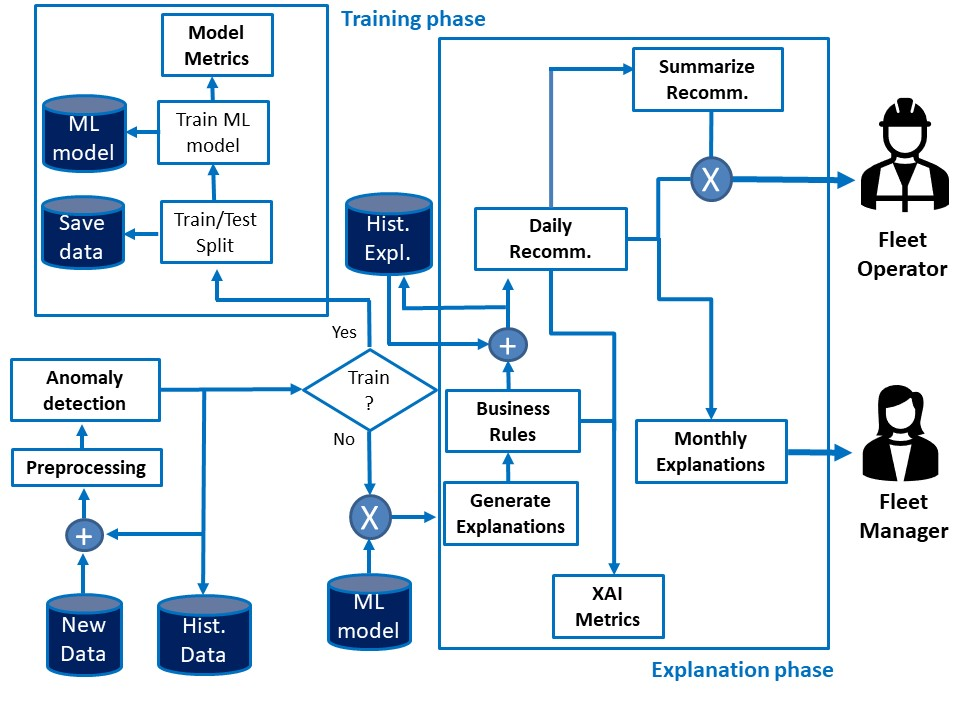
\includegraphics[width=320pt]{figures/chapter6_LucaFleet/FlowchartFinal.jpg}
  \end{tabular} 
  \caption{General flowchart followed by the fuel RecSys, as described in \hyperref[subsec:ch6-process-overview]{Subsection} \ref{subsec:ch6-process-overview}}
  \label{fig:ch6-flowchart-fuel-recsys}
\end{figure*}

Then, the process either applies the training phase for creating a new ML model, or applies the explanation phase, using one previously trained. 
For the training phase, the process trains an interpretable ML model \hyperref[subsec:ch6-ml-model]{Subsection} \ref{subsec:ch6-ml-model} and obtains its metrics in terms of model performance \hyperref[subsec:ch6-model-metrics]{Subsection} \ref{subsec:ch6-model-metrics}.

For the explanation phase, the process loads the ML model already trained, and uses it for generating explanations over the new data. They are combined with business rules in order to assure a minimum explanation quality \hyperref[subsec:ch6-business-rules]{Subsection} \ref{subsec:ch6-business-rules}. The explanations are stored and combined with previously generated ones. Then, they are used for generating daily recommendations that show the potential fuel that could be saved for each vehicle \hyperref[subsec:ch6-daily-recommendations]{Subsection} \ref{subsec:ch6-daily-recommendations}. The explanation phase also includes XAI metrics that can be used both for comparing the explanations generated by different models, as well as for measuring their quality by themselves \hyperref[subsec:ch6-xai-metrics]{Subsection} \ref{subsec:ch6-xai-metrics}.

Finally, the fuel saving recommendations are adjusted considering the audience that will receive them. There are two types of audiences considered for this purpose; a) \textbf{fleet operators} that receive the information about individual vehicles that have anomalous fuel consumption, together with recommendations that can be applied for reducing it; b) \textbf{fleet managers} that receive general explanations about the impact of driving behaviour features in the fuel consumption of the whole fleet, as well as information about the fuel consumption of vehicle models without taking into consideration the extra amount caused by the inefficient driving style \hyperref[subsec:ch6-recomm-user-profiles]{Subsection} \ref{subsec:ch6-recomm-user-profiles}. \hyperref[fig:ch6-ExplanationsDashboardExample]{Figure} \ref{fig:ch6-ExplanationsDashboardExample} shows an example of the final output explanations for those two user profiles. 

\begin{figure*}
\centering
  \begin{tabular}{c@{\qquad}c@{\qquad}c}
  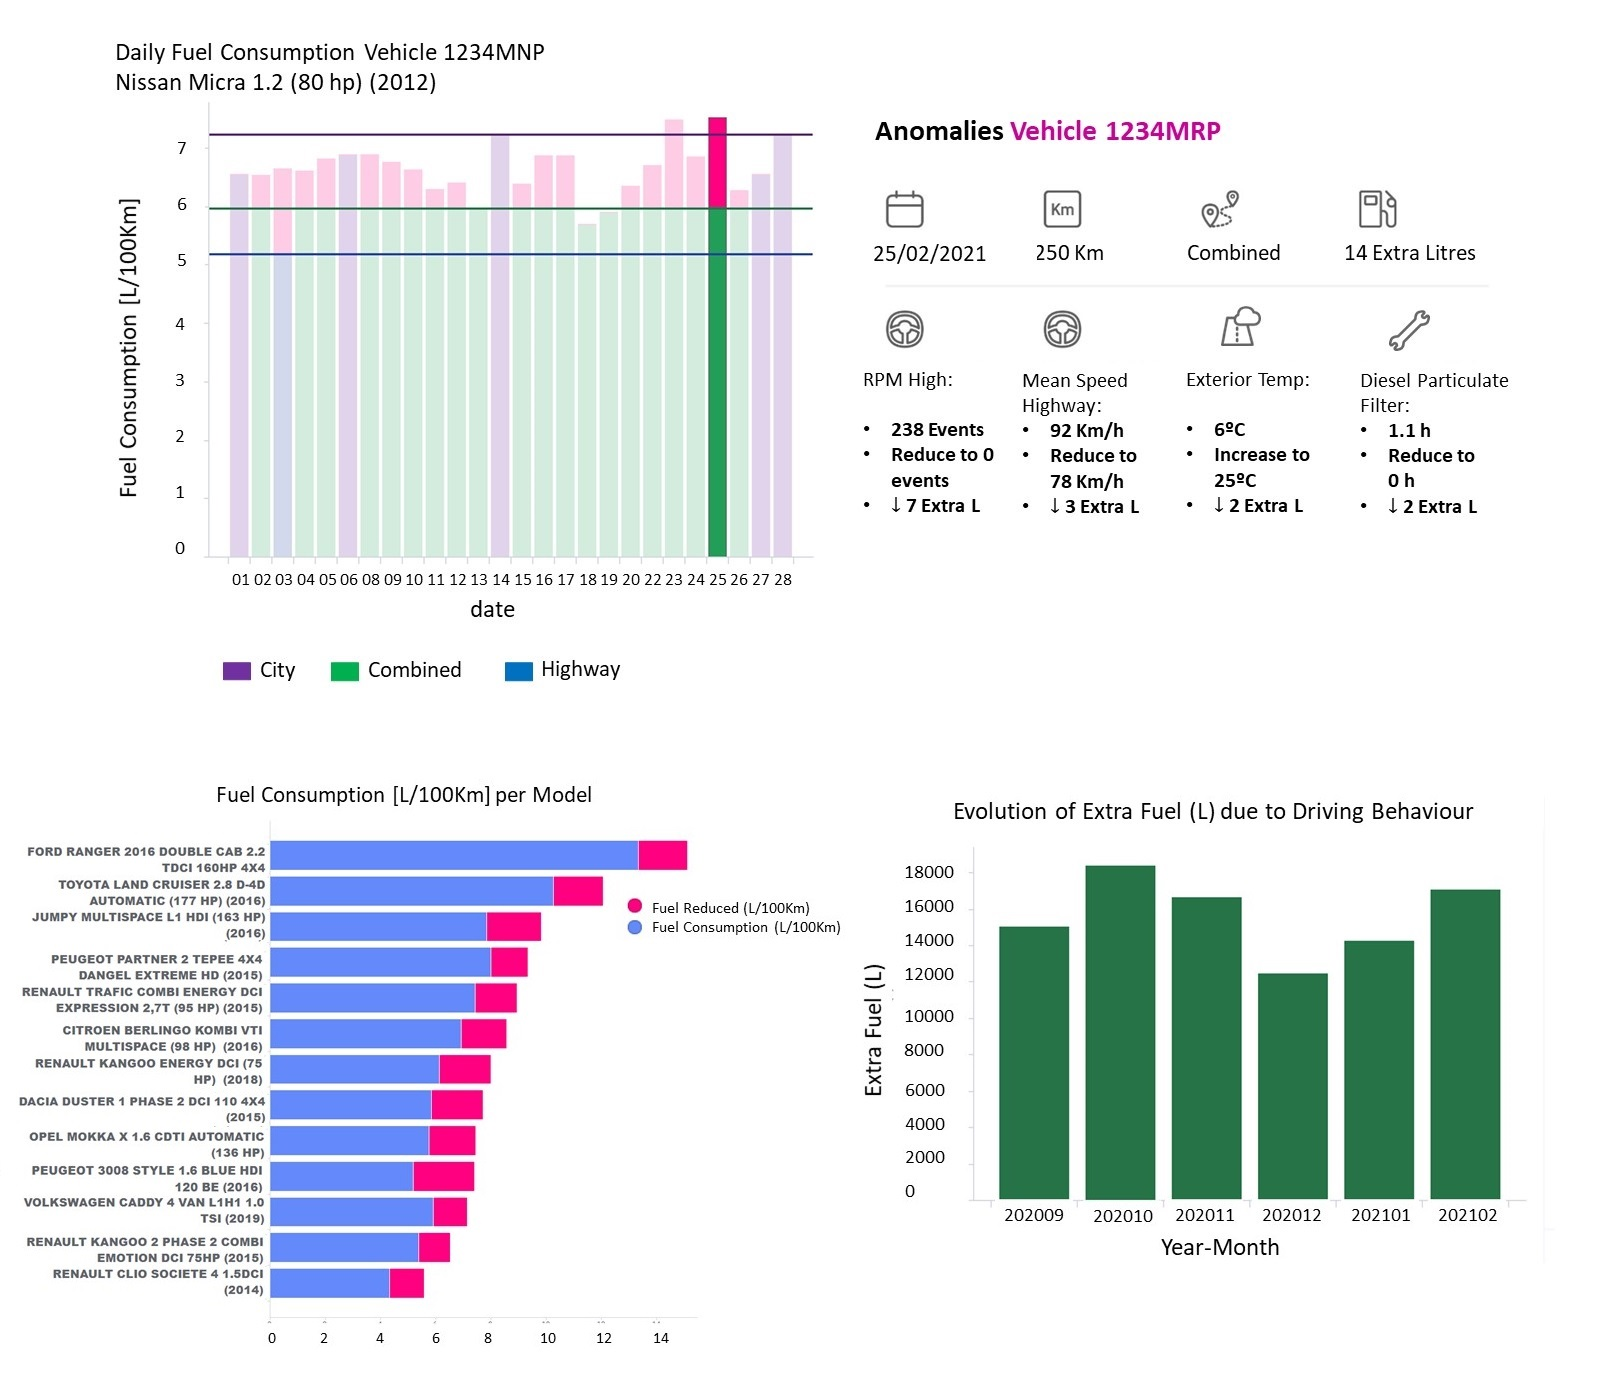
\includegraphics[width=0.9\columnwidth]{figures/chapter6_LucaFleet/ExplanationsDashboardExample.jpg}
  \end{tabular} 
  \caption{Example of explanations and recommendations for Fleet Operators (above) and Fleet Managers (below).\label{fig:ch6-ExplanationsDashboardExample}}
\end{figure*}

\subsection{Data preprocessing}\label{subsec:ch6-data-processing}
First, we obtain the daily aggregated information for each of the vehicles within the fleet through the telematics devices connected to the OBD-II (On-Board Diagnostics) on each of them. This generates real-time information of the vehicle's status. A sample of these raw data with a csv structure can be seen in \hyperref[table:ch6-sample-structure]{Table} \ref{table:ch6-sample-structure}.

\begin{table}[h!]
\centering
\resizebox{350pt}{!}{%
\begin{tabular}{llll}
\textbf{time\_tx} & \textbf{vehicle\_id} & \textbf{variable\_id} & \textbf{variable\_value} \\ \hline
2020-10-31 00:02:34.073000+00:00 & b123 & EngineSpeed  & 1200 \\
2020-10-31 00:12:34.073000+00:00 & b124 & VehicleSpeed & 55   \\
2020-10-31 01:12:34.073000+00:00 & b125 & EngineSpeed  & 1200 \\
2020-10-31 02:02:34.073000+00:00 & b124 & TripFuel     & 3.1 
\end{tabular}
}
\caption{Sample of the received data from the telematics devices}
\label{table:ch6-sample-structure}
\end{table}

We are interested in a daily vision of the vehicle for providing recommendations for the user profiles with a daily granularity level. Thus, we aggregate the raw information into a set of features, described at \hyperref[sec:annex-fuel-features]{Section} \ref{sec:annex-fuel-features} in the \hyperref[ch:annex]{Annex}. The features chosen correspond to a domain prior knowledge, since they must be related to vehicle's fuel consumption \parencite{zacharof2016review}. These features appear within the literature as potential causes of increased fuel usage both from the driving behaviour influence in fuel economy \parencite{zhang2017safedrive}, as well as from the vehicle status and exterior conditions \parencite{zhou2016review}. These features have already been proven useful for predicting fuel consumption with ML models \parencite{9072728, 8727915, perrotta2017application, barbado2021understanding}.

The features are divided into 4 groups: Index, Categorical, Explainable and Target. They are described below (though, for more detail, we refer to \hyperref[sec:annex-fuel-features]{Section} \ref{sec:annex-fuel-features} in the \hyperref[ch:annex]{Annex} \ref{ch:annex}).

\begin{itemize}
    \item \emph{Index features} refer to features used to identify each row (namely a vehicle's unique id, and the date).
    \item \emph{Categorical features} refer to non-numerical features used to distinguish group of vehicles, such as "vehicle model", which indicates vehicles with the same make-model, or "route type" for identifying the primary route type on a specific date (highway, city or combined). 
    \item Regarding the \emph{Explainable Features}, they are further divided into six groups. First, there are features related to the vehicle status itself. For instance, the pressure of the tires. If the pressure is too low, the fuel needed to cover the same amount of distance will increase, thus increasing the fuel consumption of the vehicle. These features are identified as \emph{vehicle condition}. 
    The next group of features are the \emph{Driving Behaviour} ones. They correspond to features related to the vehicle's driver behaviour itself that may affect the fuel consumption. An example of these features is the idle time spent. More idle time may increase fuel consumption.
    Another group of features considered are the \emph{Weather Variables}. For instance, the exterior temperature may affect a vehicle's thermodynamic cycle, harming its efficiency. Related to that, there is another group of features, called \emph{Road Conditions} for addressing the driving context (e.g. the time driving in a road with bumps). The final two groups are features related to the \emph{Operational Mass} of the vehicle, and to the extra fuel consumption from the usage of \emph{Auxiliary Systems} (e.g. time with air conditioning on). 
    \item The final feature is the \emph{target} column, the fuel consumption itself. This is calculated directly as: 
    \begin{equation}
    fuel\;consumption\;(L/100Km) =  \frac{trip\;fuel\;used\; (L)}{trip\;distance\;(kms)} \times 100
    \end{equation}\myequations{Vehicle fuel consumption}
\end{itemize}

This yields a data frame where each row corresponds to the daily aggregated values of the selected features for a specific vehicle. 

\subsection{Unsupervised anomaly detection in vehicle fuel consumption}\label{subsec:ch6-anomaly-detection}
Using the previous FAR data frame, the next step detects the vehicle-dates where there is an anomalous fuel consumption. Since there is no prior knowledge on when the fuel consumption is anomalous, we need to detect it in an unsupervised manner. Also, the module needs to provide a threshold value to distinguish outliers from inliers, since we want to include that information as a visual explanation.

To comply with both requirements, we apply an univariate unsupervised anomaly detection approach using a Box-Plot that classifies data points as outliers if they are above or below a specific threshold. \hyperref[eq:ch6-boxplot-anomalies]{Equation} \ref{eq:ch6-boxplot-anomalies} shows these thresholds using a 1.5 multiplier, which corresponds to approximately $\pm2.7\sigma$ (where $\sigma$ is the standard deviation) and 99.3\% coverage of the data for a normal distribution \parencite{mcgill1978variations, krzywinski2014visualizing}. This approach, with the 1.5 standard multiplier, has already been used within other vehicle-related contexts for anomaly detection in the energy usage \parencite{yin2019voltage, schuster2015lithium}.

In our case, the Box-Plot is applied over the different combinations of the categorical variables (make-model with vehicle\_group and route type with route\_type), obtaining different limits depending on the combination considered. We use this approach since the fuel consumption of a vehicle will change depending on the route type (e.g. city vs highway) and depending on the vehicle model \parencite{rakha2011virginia, zacharof2016review}.

\begin{equation}\label{eq:ch6-boxplot-anomalies}
\begin{split}
lim\_sup = Q3 + 1.5 \times IQR \\
lim\_inf = Q1 - 1.5 \times IQR
\end{split}
\end{equation}\myequations{Boxplot limits for anomaly detection in vehicle fuel consumption}

\subsection{ML model for generating for connecting input features and fuel consumption}\label{subsec:ch6-ml-model}
The following step is the training of a ML supervised model that finds relationships between the explainable and categorical features from the FAR data set and the target variable. Within this step, we could use any whitebox model that yields feature relevance-based global explanations. The main proposal is based on EBM \parencite{nori2019interpretml}, since its a whitebox algorithm with good predictive power that has been previously used within the fuel consumption context \parencite{barbado2021understanding}. With that, we have an interpretable model that can provide explanations about the relationship between input features and output fuel consumption, while being able to model complex non-linear relationships.

However, there are two problems that arise with EBM within the context of fuel consumption. First, the feature relevance explanations will be the same for all the vehicles within the fleet. That means that the unitary impact from, for instance, one extra speeding event, will be the same for passenger cars than for trucks if the fleet contains both types of vehicles. This could be fixed by using the pairwise terms of EBM to adjust each feature. For instance, $f_i(x_i) + f_ij(x_i, x_j)$ will be the adjusted feature relevance value for feature $x_i$ considering the vehicle model $x_j$. The problem is that we will need to adjust every combination of features and vehicle models, and this will significantly increase the number of features used for training the ML model. Our proposal for this problem is addressed with our EBM variation (EBM\_var) algorithm, which is detailed later.

Another problem is that the relationship between feature values and feature relevance may not be monotonic when it should be. For instance, more time driving in idle mode should always lead to more fuel consumption, and not to less. The original proposal of EBM does not allow for the usage of monotonic constraints. Because of that, we will also evaluate the usage of the CGA2M+ algorithm \parencite{watanabe2021cga2mplus}, where we can specify monotonic constraints. An example of these problems is shown in \hyperref[fig:ch6-ProblemsEBM]{Figure} \ref{fig:ch6-ProblemsEBM}.

\begin{figure}[h!]
\centering
  \begin{tabular}{c@{\qquad}c@{\qquad}c}
  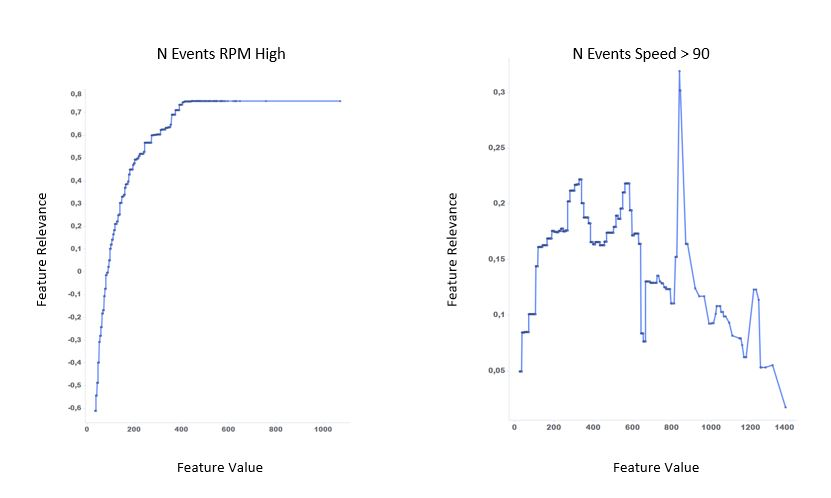
\includegraphics[width=300pt, height=180pt]{figures/chapter6_LucaFleet/ProblemsEBM.jpg}
  \end{tabular} 
  \caption{Problems with EBM. Left, we see that even though the evolution is monotonic by directly using EBM, the model uses one pairplot for every model in the fleet. Right, we see an example of a pairplot that should be monotonic but it is not.}
  \label{fig:ch6-ProblemsEBM}
\end{figure}

Our final solution will use the proposal that yield best results, according to the metrics defined at \hyperref[subsec:ch6-metrics]{Subsection} \ref{subsec:ch6-metrics}. % TODO, dejarlo así o hablar de que usamos EBM\_var?

\textbf{EBM variation}\label{subsec:ch6-ebm-var-intro}\\
The EBM variation that we propose considers possible differences that may exist within different subgroups of vehicles in order to adjust feature relevance and predictions. Regarding our use case, the feature relevance may be different depending on the vehicle group. For instance, the impact on the fuel consumption for each additional harsh brake may change depending on the vehicle's model and make considered. Thus, there should be different feature relevance-values pairs depending on that vehicle group category. Using only one EBM provides unique pairs of value-relevance regardless of the vehicle group, meaning that the final impact in the target variable will be the same for a specific feature value.

The intuition behind our proposal is similar to other works in the literature \parencite{waeto2017forecasting}. We add an additional layer of models to predict the error of a previous one. As represented in \hyperref[fig:ch6-ebm-variation-flowchart]{Figure} \ref{fig:ch6-ebm-variation-flowchart} for one subgroup of vehicles, first, we train an EBM model over all data during the training phase. Then, we predict the error for each of the vehicle's subgroups, and train additional EBM to predict that error and both improve the predictions of the first one as well as adjusting the results to the specificity of each of the subgroups. This last consideration is based on the fact that while the first model provides unique feature relevance-values pairs (because the second one is predicting the error of the first one in order to add it to its prediction), we can also use the feature relevance values of the second one to add them to the first one. This may be done since the feature relevance values of the second model show the feature contribution to the error.
With that, there will be different feature relevance-value pairs, as well as predictions, for each of the subgroups considered.

\begin{figure}[h!]
\centering
 \begin{tabular}{c@{\qquad}c@{\qquad}c}
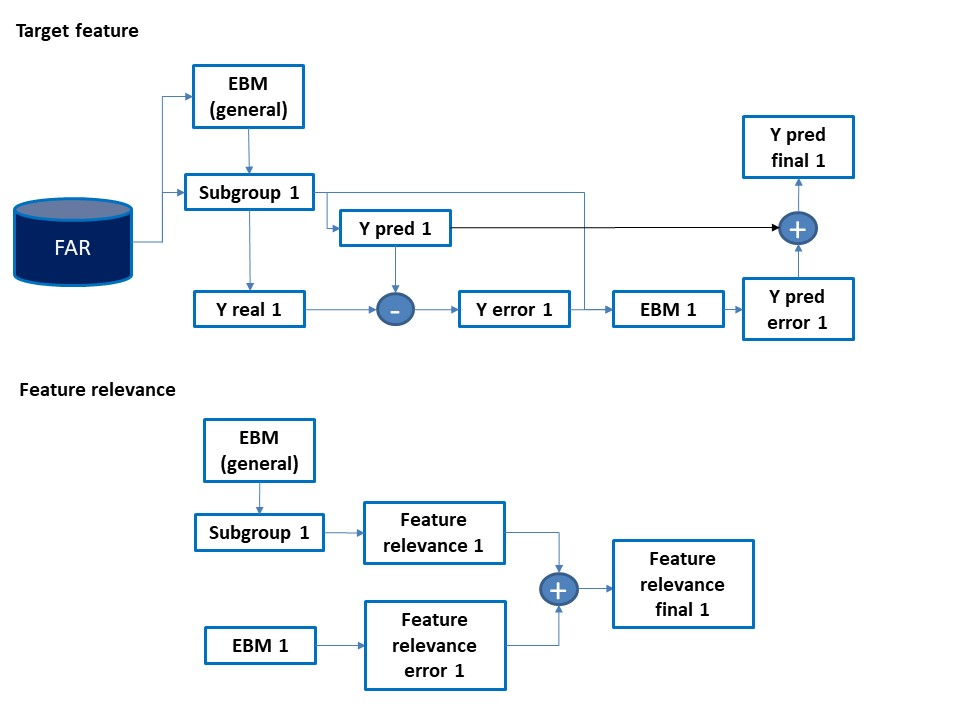
\includegraphics[width=280pt, height=200pt]{figures/chapter6_LucaFleet/EBM_variation.jpg}
  \end{tabular} 
  \caption{Proposal of the "EBM variation" over only one subgroup.  \label{fig:ch6-ebm-variation-flowchart}}
\end{figure}

The detailed description of EBM variation appears at \hyperref[subsec:annex-ebm-var]{Subsection} \ref{subsec:annex-ebm-var} in the \hyperref[ch:annex]{Annex}. 

\subsection{Generate explanations}\label{subsec:ch6-generate-explanations}
The "Generate explanations" step extracts the relationship between the fuel consumption of a vehicle in a specific date and the input features (FAR). This relationship is expressed in
\hyperref[eq:ch6-y-pred]{Equation} \ref{eq:ch6-y-pred}.

\begin{equation}\label{eq:ch6-y-pred}
y\_pred (n) = \varepsilon + \sum_{i=1}^{k}  f_{i}(x_{i}(n))
\end{equation}\myequations{Vehicle fuel consumption prediction based on the EBM output}

\hyperref[eq:ch6-y-pred]{Equation} \ref{eq:ch6-y-pred} shows the relationship for a data point \textit{n} between the predicted value of the target variable y\_pred with respect to \textit{k} input features, $x_{i}$, through their $f_{i}(x_{i}(n))$ functions. Thus, for a specific data point $n$ and feature value $x_{i}(n)$, we get the corresponding feature relevance $f_{i}$, obtaining the individual contribution of that feature in that data point to the predicted fuel consumption.
In all the cases, we train models without using pairwise terms, since they will potentially make the explanations and recommendations too complex. Thus, the explanations will not consider the joint evolution of two features (e.g., the joint evolution of a feature like 'mean exterior temperature' with 'hours raining', even though they may be related).

\subsection{Business rules}\label{subsec:ch6-business-rules}
Over the raw explanations, we apply the following business rules:
\begin{itemize}
\item \textbf{BR1}: The features used for training the model may be numeric (e.g. time driving uphill) or categorical (e.g. the vehicle model). All those categorical features are one-hot encoded before training the model. However, they are not considered for the explanations since they are not actionable (e.g., changing the vehicle model may lead to less fuel consumption under the same circumstances, but it is not something that can be acted upon easily in order to change it. Opposed to this are actionable features, like 'harsh brakes', which can be changed more easily from one day to another).
\item \textbf{BR2}: We remove the features in the vehicle-date explanations that have a very low impact on the fuel consumption (relative impact below 1\%)
\item \textbf{BR3}: The explanations only include vehicles where the average fuel consumption is above the value of the median inlier vehicles for the same model and on the same route type.
\item \textbf{BR4}: Feature values must be higher than the median value of the vehicle inliers from the same model for that same feature when the feature Type is Positive, or lower when Type is Negative.
\item \textbf{BR5}: The total fuel reduction from the explanations should not be more than the 80\% of the original fuel consumption\footnote{The value of 80\% is decided based on \hyperref[table:ch2-sota-FeatureInfluenceReduced]{Table} \ref{table:ch2-sota-FeatureInfluenceReduced} and \parencite{zacharof2016review}: considering the mean fuel reduction per category, using the upper limit values, we get a potential maximum reduction of 89.1\%. Since considering all the features together with their maximum contribution is an extreme case, we have validated with domain experts to set it to 80\%}. Since the models do not allow to impose restrictions in the learning for the individual models for the features, we need to apply this post-hoc filtering to remove explanations that are not physically possible.
\end{itemize}
EBM and EBM\_var do not necessarily yield monotonic explanations for each feature. Because of that, in this step we include an optional monotonicity filter in order to filter some of the feature relevance - feature values combinations from among all vehicles, and leave only those that result in a monotonic relationship between them. This filtering is optional, and can be used both for selecting only some particular explanations, or for computing a monotonicity metric that measures the degree of monotonicity for each feature in the data set \hyperref[subsec:ch6-xai-metrics]{Subsection} \ref{subsec:ch6-xai-metrics}. 

The \textbf{Monotonicity filter} analyses each pair of feature value and feature relevance for every vehicle group and route type combination and discards the pairs that are not monotonic. An example can be seen in \hyperref[fig:ch6-monotonicity-filter-example]{Figure} \ref{fig:ch6-monotonicity-filter-example}.
Starting from the evolution of the relevance-value pair of a particular feature, in this step the process finds the feature values intervals where the feature relevance is not monotonic, and discards those combinations. Thus, the raw explanations for each vehicle-day, where all the features are included, are filtered so that the feature values that correspond to feature relevance ones that are not monotonic are not included. 
\hyperref[fig:ch6-monotonicity-filter-example]{Figure} \ref{fig:ch6-monotonicity-filter-example} shows the original feature relevance-value pairs for a combination of route type and vehicle group for the feature count\_harsh\_brakes. As the figure shows, the evolution is not monotonic. It also shows the final result after applying the monotonicity filter.

\begin{figure}[h!]
\centering
 \begin{tabular}{c@{\qquad}c@{\qquad}c}
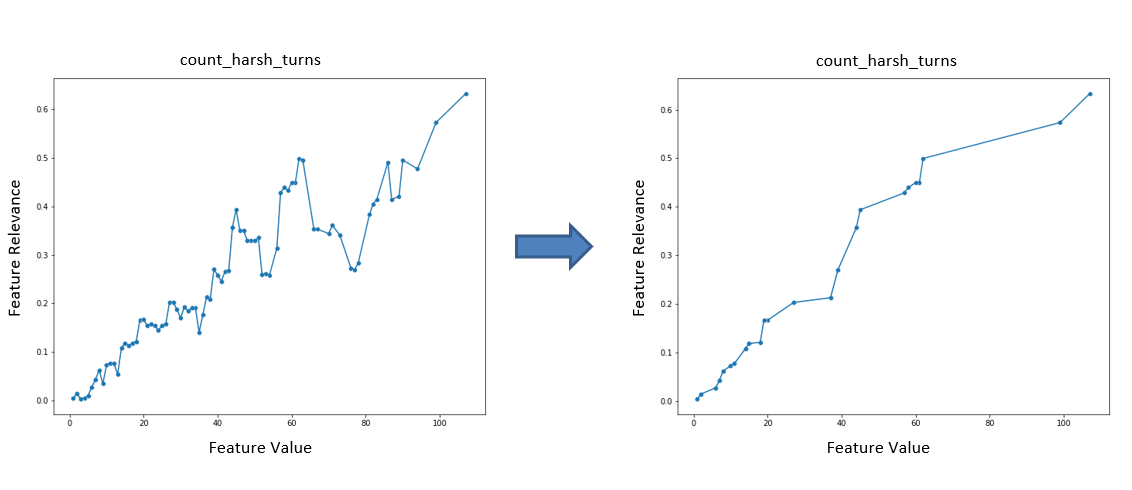
\includegraphics[width=350pt]{figures/chapter6_LucaFleet/MonotonicFilterExample.PNG}
  \end{tabular} 
  \caption{Example of evolution of the feature value and the feature relevance for feature count\_harsh\_brakes before and after applying the monotonicity filter\label{fig:ch6-monotonicity-filter-example}}
\end{figure}

A detailed description of the algorithm appears within the \hyperref[subsec:annex-monotonicity]{Subsection} \ref{subsec:annex-monotonicity} in the \hyperref[ch:annex]{Annex}. Since the monotonicity filter analyses the combined evolution of both feature relevance and feature value, it works either for EBM (where there is only one value-importance pair per feature at the dependency function \parencite{nori2019interpretml}), EBM\_var (where there is potentially one value-importance pair per feature and vehicle group), as well as with other XAI algorithms such as LIME and SHAP (where there may be more than one importance value per unique feature value \parencite{molnar2019interpretable}). Indeed, there may be more than one importance-value pair per feature value. However, since \hyperref[subsec:annex-monotonicity]{Subsection} \ref{subsec:annex-monotonicity} checks a pair and the immediate following one, it will, for instance, check $(x0,y0)$ against $(x0, y1)$ with $y1 > y0$, and will remove the latter if the importance is lower.

This approach is known as \textit{Informed Explainability} within the taxonomy of \parencite{beckh2021explainable}, since we are applying the prior knowledge not over the underlying blackbox model (the anomaly detection algorithm in this case), but over the XAI method itself. In particular, our approach works with \textit{formalized priors for explanations} since the knowledge is elicited through the literature, instead of using other approaches such as human-on-the-loop.

\subsection{Daily recommendations}\label{subsec:ch6-daily-recommendations}
Whitebox models that include feature relevance are useful for counterfactual explanations \parencite{arrieta2020explainable}. Since there is a unique intercept and unique feature relevance-value pairs, they can provide counterfactual explanations where one of the feature values alone may be changed, recalculating the predicted target value to see how it will change. These counterfactual explanations can be used as recommendations since they show future scenarios when particular actions take place.

The intuition behind it is the following one. "Generate Recom." changes the feature values of the outliers used within the explanation phase to a reference value (e.g. the corresponding median feature value of the inliers belonging to the same vehicle group and route type). This is applied for one feature at a time and for every feature labeled as "actionable" \footnote{As already mentioned, changing a feature like the vehicle model may lead to less fuel consumption under the same circumstances, but it is not something that can be acted upon easily in order to change it. Opposed to this are actionable features, like 'harsh brakes' or 'jackrabbits', which can be changed more easily from one day to another. These features were decided with the input received from domain experts}. Then, by subtracting the relative change in the predicted value from the real fuel consumption, it indicates which vehicles-dates would have a fuel consumption below the outlier limit for that vehicle group and route type. 

The details are described in \hyperref[alg:ch6-get-recom]{Algorithm} \ref{alg:ch6-get-recom}; getRecom function receives the historical median values of the inliers (obtained during the training phase; $X_{med}$), the data points of the explanation phase with their feature relevance ($X_{exp}$), and two lists, one with the explainable features that are actionable ($l_a$) and one with the categorical ones ($l_c$). It also receives a list $l_z$ with the features that are going to be explained using a zero value reference (for instance, by reducing the "harsh brakes" to zero, instead of the median value for that vehicle group). Using these inputs, getRecom function initializes two empty lists ($l\_up\_ind$ and $l\_up\_all$) and gets the feature relevance for the median inliers feature values ("coeff"), or zero value, with $checkPairwise(X_{med}, l_c, l_z)$ function. 
After obtaining the feature relevance, the function analyses every data point ($x$) within the explanations and obtains its predicted target value ($y\_pred$) using the feature relevance and the intercept. It also stores the real value ($y\_real$) of the target feature. Then, it checks every feature ($f$) within the explanations and gets its corresponding feature relevance from the median inliers reference, or the zero value reference, ($\beta_{fn}$). Then, it sums again all the feature relevance and intercept for data point x, without the feature relevance for feature "f". This leads to a new predicted value ($y\_new$) where all the other feature values are kept the same, but but with a change on the specific feature considered. The difference between $y\_pred$ and $y\_new$ is $\Delta$, and this difference is used to compute the change in the real fuel consumption ($l\_up\_ind$). After iterating for all the available combinations, getRecom uses groupVal function to obtain the estimated value in case all the actionable features change at the same time to their references (either zero or their median inlier value). This is done by aggregating all the individual changes in the prediction for each feature and subtracting the aggregated difference from the real fuel consumption.

% Recommendations
\begin{algorithm}[h!]
\caption{Generate Recommendations}\label{alg:ch6-get-recom}
\begin{algorithmic}[1]
\Procedure{getRecom}{$X_{med}, X_{exp}, l_a, l_c, l_z$}
    \State $l\_up\_ind \gets null$
    \State $l\_up\_all \gets null$
    \State $coeff \gets checkPairwise(X_{med}, l_c, l_z)$
    \For{$x \in X_{exp}$}
        %\State $y\_pred \gets \varepsilon + \sum_{i=1}^{k}  \beta_{i}(x_{i}) \times x_{i} $
        \State $y\_pred \gets \varepsilon + \sum_{i=1}^{k}  F_{i}(x_{i}) $
        \State $y\_real \gets x[target]$
        \State $comb \gets x[l_c]$
        \For{$f \in l_a$}
            \State $\beta_{fn} \gets coeff[f]$
            %\State $y\_new \gets \varepsilon + \sum_{i=1}^{k \neq f}  \beta_{i}(x_{i}) \times x_{i} $
            \State $y\_new \gets \varepsilon + \sum_{i=1}^{k \neq f}  F_{i}(x_{i})$
            %\State $y\_new \gets y\_new + \beta_{fn} \times X_{med}[comb]$
            \State $y\_new \gets y\_new + \beta_{fn}$
            \State $\Delta \gets y\_pred - y\_new$
            \State $y\_updated \gets y\_real - \Delta$
            \State $l\_up\_ind \gets l\_up\_ind.append(y\_updated)$
        \EndFor
    \EndFor
    \State $l\_up\_group \gets groupVal(l\_up\_ind, l_a, X_{exp}, l_c)$
    \State \textbf{return} $l\_up\_ind, l\_up\_group$
\EndProcedure
\end{algorithmic}
\end{algorithm}

Thus, \hyperref[alg:ch6-get-recom]{Algorithm} \ref{alg:ch6-get-recom} provides a list with the new estimated fuel consumption value for every individual feature change and for every vehicle-date pair ($l\_up\_ind$). Comparing these values against the outlier limit for that vehicle group and route type, we can see which individual feature changes will turn outliers into inliers, and what would be the new fuel consumption. It also provides a similar result but considering that every actionable feature changes at the same time ($l\_up\_group$). 

% TODO: Puedo meter aqui la tabla de ejemplo de salida del "Understanding..."

\subsection{Recommendations according to user profiles}\label{subsec:ch6-recomm-user-profiles}
According to \parencite{arrieta2020explainable}, explanations should be tailored for the specific profile of the user that will receive them, taking into account both their expectations and their domain knowledge. Within the use case proposed in this chapter, we identify two user's profiles: fleet operators and fleet managers.

\textbf{Fleet operators} are responsible for the status of the vehicles. Their main interest in explanations is detecting what vehicles are consuming excessively, and what is causing it, considering for that not every feature, but only the ones that are actionable, according to \hyperref[sec:annex-fuel-features]{Section} \ref{sec:annex-fuel-features} in the \hyperref[ch:annex]{Annex}. To accomplish that, the recommendations generated at \hyperref[subsec:ch6-daily-recommendations]{Subsection} \ref{subsec:ch6-daily-recommendations} may be enough. However, providing information for every combination of dates, vehicles and route types in terms of the numeric feature relevance may be overwhelming, not being useful for them. Therefore, we provide the recommendations for these users at two different levels. First, a summary of the main recommendations for a specific period of time (e.g. a month), where we only show vehicles that have a recurrent behaviour that impacts in the fuel consumption (e.g. always with driving behaviour related features). Second, we provide the individual daily detail only if they want to dive deeper into a particular vehicle and route type. In both cases, we only include vehicles with fuel consumption anomalies.

For the other profile, \textbf{fleet managers}, the main interest is having a global comparative view at a vehicle model level, not seeing information about individual vehicles or specific dates. Explanations should be expressed in terms of extra litres of fuel consumed, because that can be immediately turned into an economic cost, as well as in terms of environmental impact. For this profile, it is also useful not to consider all types of features in the explanations, but only the ones related to driving behaviour, since they are among the features with more impact \parencite{zacharof2016review}, they are actionable, and they are mainly associated to inefficient driving styles.
With that, after having the individual recommendations from \hyperref[alg:ch6-get-recom]{Algorithm} \ref{alg:ch6-get-recom}, the individual explanations are aggregated for the whole fleet and for each vehicle model, considering only for the potential fuel reduction features related to driving behaviour. A final comment is that these explanations include all data points, not only the outliers since it is an aggregated view.

\subsection{Metrics}\label{subsec:ch6-metrics}
There are two aspects to measure through metrics: model performance and quality of the explanations/recommendations. For the first case, we measure the predictive power of the surrogate ML model by seeing how close the predictions to the real fuel consumption value of the different vehicle-dates are. We will further refer to them as \textit{model metrics}. 

The second group of metrics are the ones obtained during the explanation phase, which are used for assessing several quality aspects within both the explanations and the final fuel saving recommendations. These metrics are useful for analysing the explanations by themselves, as well as for comparing the explanations generated between every model. We will further refer to them as \textit{XAI metrics}. Even though it may be difficult (or not reliable) to compare individual explanations from different models with certain metrics due to Rashomon's Effect \parencite{molnar2019interpretable}, the metrics that we propose analyze the explanations from a general perspective.

\subsubsection{Model performance metrics}\label{subsec:ch6-model-metrics}
\leavevmode\newline
Model metrics include metrics used for comparing the models among themselves. Here we use a test set to evaluate the model performance metrics. For that, we use we use the Adjusted R2 value (adj-R2) and the Mean Average Percentage Error (MAPE). We use adjusted R2 and MAPE, since they both yield a result in terms of percentage that can be easily understood.

All the model metrics are evaluated over a test set that includes both outliers and inliers, since the purpose is to measure how close the target feature predictions are to the real value. There are other potential metrics that can be considered, especially classification metrics that measure if after applying the anomaly limits over the predicted values, the inlier/outlier predicted class matches the one of the real target feature. However, since we are not using the ML surrogate model to actually predict the outlier/inlier class, we did not use them. 

\subsubsection{XAI metrics for assessing explanation quality}\label{subsec:ch6-xai-metrics}
\leavevmode\newline
Using the taxonomy of metrics in \parencite{carvalho2019machine} for individual explanations, we consider different properties for comparing the explanations generated by the different methods studied in this chapter. The properties considered are \textit{representativeness}, \textit{precision}, \textit{stability}, \textit{contrastiveness} and \textit{consistency with apriori beliefs} (as discussed in \hyperref[sec:ch2-metrics-xai]{Section} \ref{sec:ch2-metrics-xai}), since they address the main aspects of our use case. For stability and precision, we use metrics based on already existing metrics within the literature. For representativeness, contrastiveness and consistency with apriori beliefs, we propose additional ones that are useful for benchmarking the models within our use case. 
These metrics are used for evaluating the final explanations provided by the system (after applying all the business rules mentioned in the previous subsections unless otherwise indicated), and they are evaluated for anomalous vehicle-dates only. A summary of these metrics appear in \hyperref[table:ch6-xai-resume-metrics]{Table} \ref{table:ch6-xai-resume-metrics}.

\textbf{Representativeness} metrics measure the relevance or importance of the explanation. They include these metrics:
\begin{itemize}
    \item \textbf{n\_features}: Number of features used for fuel explanations for a particular vehicle-date. The metric appears in \hyperref[eq:ch6-xai-metrics-n-features]{Equation} \ref{eq:ch6-xai-metrics-n-features}, where $v$ is one vehicle, $t$ one date, $X^{'}(v,t)$ the remaining features after applying the business rules, and $card$ the cardinality.
    \item \textbf{rel\_importance}: Percentage of fuel covered by the features used in the explanations. The metric appears in \hyperref[eq:ch6-xai-metrics-rel-imp]{Equation} \ref{eq:ch6-xai-metrics-rel-imp}, with $f_{i}$ the dependency function for feature $i$, $\beta_0$ the intercept, and  $\beta_i$ the feature coefficient.
\end{itemize}

\begin{equation}\label{eq:ch6-xai-metrics-n-features}
\begin{aligned}
n\_features_{v,t} = card(X^{'}(v,t))
\end{aligned}
\end{equation}

\begin{equation}\label{eq:ch6-xai-metrics-rel-imp}
\begin{aligned}
rel\_importance_{v,t} = \frac{\beta_0 + \sum_{i=0}^{n\_features_{v,t}} {\beta_i \times f_{i}(x_{v,t})}} {y\_r(v,t)}
\end{aligned}
\end{equation}

\textbf{Precision} metrics measure how close is the fuel prediction to the real fuel value using the features within the explanations. For that, we use the MAPE (mean average percentage error) obtained by comparing that fuel prediction based on the final explanations against the real fuel consumption value. The metric appears in \hyperref[eq:ch6-xai-metrics-xai-mape]{Equation} \ref{eq:ch6-xai-metrics-xai-mape}, where $N_t$ are the number of data points for that vehicle $v$, $y\_p^{'}(v, t)$ the fuel prediction using the features remaining after the business rules, and $y\_r(v,t)$ the real fuel value for that vehicle and date.

\begin{equation}\label{eq:ch6-xai-metrics-xai-mape}
\begin{aligned}
xai\_mape_{v} =  \frac{\sum_{t=0}^{N_t} {mape(y\_p^{'}(v, t), y\_r(v,t))} } {N_t}
\end{aligned}
\end{equation}

\textbf{Stability} metrics include one metric, \textit{stability\_error}. This metric is based on the proposal of \parencite{melis2018towards}, as indicated in \hyperref[eq:ch6-stability-metric-sample]{Equation} \ref{eq:ch6-stability-metric-sample} within \hyperref[sec:ch2-metrics-xai]{Section} \ref{sec:ch2-metrics-xai}. For this particular metric, we do not filter the explanations using the business rules.

\begin{equation}\label{eq:ch6-stability_metric_sample}
\qquad 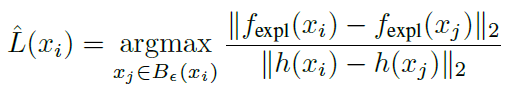
\includegraphics[width=200pt]{figures/stability_metric.PNG}
\end{equation}

\textbf{Contrastiveness} metrics measure the impact of the recommendations generated over the explanations provided by the XAI technique. These metrics are:
\begin{itemize}
    \item \textbf{per\_var}: Percentage of fuel saved for a particular vehicle-date after applying the recommendations provided by the system. It appears at \hyperref[eq:ch6-xai-metrics-per-var]{Equation} \ref{eq:ch6-xai-metrics-per-var}, where the numerator is the output from \hyperref[alg:ch6-get-recom]{Algorithm} \ref{alg:ch6-get-recom} for a vehicle $v$ and a date $t$ represented through $x(v,t)$, and the denominator $y\_r(v,t)$ is the real fuel value for that vehicle and date.
    \item \textbf{per\_below}: Percentage of anomalous vehicle-dates, within each vehicle model, that receive fuel recommendations that would change their fuel value below the anomaly threshold value.
\end{itemize}

\begin{equation}\label{eq:ch6-xai-metrics-per-var}
\begin{aligned}
per\_var_{v,t} = \frac{getRecom({X_{med}, x(v,t), l_a, l_c, l_z})[0][0]} {y\_r(v,t)}
\end{aligned}
\end{equation}\myequations{XAI metrics: contrastiveness}

\textbf{Consistent with Apriori Beliefs} metrics measure how aligned are the explanations with prior domain knowledge. It includes the following metrics:
\begin{itemize}
    \item \textbf{per\_mon}: Percentage of data points for a particular feature and model that are monotonic after applying the monotonicity filter, described in \hyperref[alg:annex-monotonicty]{Algorithm} \ref{alg:annex-monotonicty} in the \hyperref[ch:annex]{Annex}. The details for this metric are within that subsection, at
    \hyperref[eq:annex-xai-metrics-mono]{Equation} \ref{eq:annex-xai-metrics-mono}.
    \item \textbf{MAPE vs reference fuel}: This metric computes the MAPE value of the new average fuel consumption (after the recommendations) against the catalog fuel reference for that model. 
    \item \textbf{\% below catalog}: It shows the percentage of vehicle-dates that are receiving a recommendation that turns the average fuel consumption (L/100Km) below the catalog reference (with an offset of 1 L/100Km). It should be minimized, because the target fuel should not be below the catalog reference (a value that is not physically reachable). 
\end{itemize}


\begin{table}[h!]
\centering
\resizebox{180pt}{!}{%
\begin{tabular}{@{}lll@{}}
\toprule
\textbf{Taxonomy}  & \textbf{Metric}       \\ \midrule
Representativeness & n\_features           \\
Representativeness & rel\_importance  \\
Precision          & xai\_mape             \\
Stability          & stability\_error      \\
Contrastiveness    & per\_var              \\
Contrastiveness    & per\_below            \\
Apriori Beliefs    & per\_mon     \\
Apriori Beliefs    & mape vs reference fuel     \\
Apriori Beliefs    & per\_below\_catalog     \\
\bottomrule
\end{tabular}%
}
\caption{Summary of the XAI metrics analysed, linking them to their taxonomy.}
\label{table:ch6-xai-resume-metrics}
\end{table}


\section{Evaluation}\label{sec:ch6-evaluation}
In this section, we indicate some aspects regarding the evaluations carried out. First, we describe the data sets that we have used in \hyperref[subsec:ch6-DataFleet]{Subsection} \ref{subsec:ch6-DataFleet} and the models configuration \hyperref[subsec:ch6-model-params]{Subsection} \ref{subsec:ch6-model-params}. Then, we focus on the evaluations themselves along with the hypothesis checked in \hyperref[subsec:ch6-eval-model-performance]{Subsection} \ref{subsec:ch6-eval-model-performance} for the evaluations regarding model performance, and in \hyperref[subsec:ch6-eval-xai]{Subsection} \ref{subsec:ch6-eval-xai} and \hyperref[subsec:ch6-eval-xai-apriori]{Subsection} \ref{subsec:ch6-eval-xai-apriori} for the XAI evaluations.

Our aim is to use this analysis for evaluating \textbf{H2} and \textbf{H1}, described in \hyperref[chap:3-objetives]{Chapter} \ref{chap:3-objetives} at
\hyperref[sec:Hypotheses]{Section} \ref{sec:Hypotheses}, within the context of vehicle fuel consumption, using our XAI proposal, which can be based on any of the three interpretable models described in \hyperref[sec:ch6-method]{Section} \ref{sec:ch6-method} (EBM, EBM\_var and CGA2M2+).

For checking \textbf{H1}, we evaluate our proposal through the XAI-specific metrics described in \hyperref[subsec:ch6-xai-metrics]{Subsection} \ref{subsec:ch6-xai-metrics}, in order to see if we can measure the quality of the explanations that indicate what features are causing that the vehicle fuel consumption is anomalous. Here, we benchmark the interpretable models alternatives in order to see if the explanations are significantly different.

Regarding \textbf{H2}, the use-case of vehicle fuel consumption is useful since there is extensive literature regarding the prior domain knowledge about what variables impact on the vehicle fuel consumption. For the evaluations of H2, we consider our proposal based on the "EBM\_var" interpretable model unless otherwise said. We analyse the following aspects:
\begin{itemize}
\item We first evaluate if there are significant differences in terms of model performance between our proposed EBM\_var and the original EBM. (\hyperref[subsec:ch6-eval-model-performance]{Subsection} \ref{subsec:ch6-eval-model-performance})
\item After that, we analyse if the model performance metrics for the three intepretable methods (EBM, EBM\_var and CGA2M2+) can be considered good enough on absolute terms. (\hyperref[subsec:ch6-eval-model-performance]{Subsection} \ref{subsec:ch6-eval-model-performance})
\item Then, we evaluate our XAI proposal, which takes into account prior domain knowledge, in order to see if the explanations generated for explaining the features that impact on the vehicles with anomalous fuel consumption are indeed aligned to that prior knowledge (\hyperref[subsec:ch6-eval-xai-apriori]{Subsection} \ref{subsec:ch6-eval-xai-apriori})
\item We also check if there are significant differences in XAI-specific metrics regarding other aspects besides prior domain knowledge. (\hyperref[subsec:ch6-eval-xai]{Subsection} \ref{subsec:ch6-eval-xai})
\item Finally, we analyse if our proposal yields similar results in terms of model performance compared to SOTA blackbox models. Thus, we see if there is a trade-off or not between an interpetable model that includes domain knowledge against a blackbox model that aims to optimize only model performance within this context. (\hyperref[subsec:ch6-eval-model-performance]{Subsection} \ref{subsec:ch6-eval-model-performance})
\end{itemize}

We will carry out an study with EBM and EBM\_var that both considers the usage of the monotonicity filter for adjusting the final explanations or not. The first analysis will not use this filtering for two reasons. First, because it is a filter that is only applicable to EBM and EBM\_var, and we want to perform a comparison against CGA2M2+ that uses the same business rules in all three cases. Second, because it will just dampen the impact of the explanations. Thus, in order to see if EBM\_var is aligned with prior domain knowledge, first we are going to see the least conservative case (with the explanations without the filter), knowing that if the full explanations are aligned with prior knowledge, since the filtered ones are a subset of them, they should also be aligned. Nonetheless, we will include a XAI metric comparison considering the explanations after the monotonicity filter.

With that, the analyses on this chapter provide a full evaluation of the sub-hypotheses described in this thesis, thus answering the main hypothesis. The reason behind it is that we evaluate the quality of explanations through XAI metrics after using domain knowledge for generating them, we  check if the explanations are aligned to that domain knowledge, and we see if there is a significant penalty on model performance or not by enforcing the explanations to follow that prior knowledge.

\subsection{Data involved}\label{subsec:ch6-DataFleet}
We consider 9 data sets, belonging to different fleets, as shown in \hyperref[table:ch6-data-description]{Table} \ref{table:ch6-data-description}. These data sets are samples for some of their vehicles, and the aggregated information includes information collected during 2019, 2020 and 2021. The table indicates the data set (Fleet), the number of individual vehicles (Vehicles), the number of vehicle groups (Models), the unique combinations of vehicle-dates (Points), the N points that are associated with an anomalous fuel consumption according to the proposal of \hyperref[sec:ch6-method]{Section} \ref{sec:ch6-method} (Outliers), and how many of those data points are within the test set (Outliers [test]). Together with that, we also include a fleet size category (Fleet Size) following the one that appears in \parencite{fleet2021trends}, where fleets with more than 500 vehicles are considered "enterprise) (or large), fleets between 50 and 499 "medium", and fleets with less than 49 vehicles "small". All the vehicles have either petrol or diesel engines.

\begin{table}[h!]
\centering
\resizebox{280pt}{!}{%
\begin{tabular}{@{}lllllll@{}}
\toprule
\textbf{Fleet} &
  \textbf{Vehicles} &
  \thead{\textbf{Fleet} \\ \textbf{Size}}&
  \textbf{Models} &
  \textbf{Points} &
  \textbf{Outliers} &
  \thead{\textbf{Outliers} \\ \textbf{[test]}}
  \\ \midrule
D1 & 1552 & Large & 16 & 219707 & 5772  & 577    \\
D2 & 1568 & Large & 16 & 121160 & 1809  & 181    \\
D3 & 316  & Medium & 44 & 65549  & 10484 & 1046   \\
D4 & 252  & Medium & 14 & 35394  & 1944  & 193    \\
D5 & 165  & Medium & 20 & 22478  & 724   & 71     \\
D6 & 143  & Medium & 20 & 18635  & 2003  & 201    \\
D7 & 33   & Small & 5  & 9733   & 949   & 95     \\
D8 & 20   & Small & 5  & 2235   & 349   & 35     \\
D9 & 3    & Small & 2  & 300    & 10    & 2      \\ \bottomrule
\end{tabular}%
}
\caption{Data set description, including the number of data points, number and type of vehicles.}
\label{table:ch6-data-description}
\end{table}

We train a model over each one of those data sets, using the 90\% of the data points for training, and the remaining 10\% for testing. As already mentioned, the model's performance metrics are analyzed considering all the test data points (comparing the model's prediction of the average fuel consumption versus the real value). For the XAI metrics used for assessing the explanations generated (the ones that appear within the explanations and recommendations from the method in \hyperref[sec:ch6-method]{Section} \ref{sec:ch6-method}), as well as for the study of explanation alignment with prior domain knowledge, we either use the whole outlier set, or we use the outlier data points that are within the test set (depending on the metric). This last aspect is indicated within every specific metric analysis.

\subsection{Model configuration}\label{subsec:ch6-model-params}
The hyperparameters used for every model match the default ones provided by the software libraries used (only modifying the parameters related to the monotonic constraints regarding CGA2M+). The reason behind that is that we ran several experiments with different hyperparameter configurations, but we did not found significant improvements from a statistical point of view in model's performance metrics when compared to the results using the default hyperparameters.  Regarding "EBM variation", both the EBM and EBM\_var use the same hyperparameter configuration.

\subsection{Model performance evaluation}\label{subsec:ch6-eval-model-performance}
In this subsection, we include the evaluations regarding the model performance. They are studied 
considering both outliers and inliers, and using the raw model predictions (without the business rules).

\subsubsection{Comparison between EBM, EBM\_var and blackbox models}\label{subsubsec:ch6-comparison-vs-blackbox}
First, we address the comparison between the different models using several model performance metrics in order to see if there are significant differences between the predictive power of the ML models analysed in this chapter. For that, we perform a k-fold cross-validation (CV) over the train data set using 30 splits. For every one of those splits, we train a model on a subset of the training data and evaluate it over the validation data selected by k-fold CV. This is done for each of those 30 splits, and for one data set per each fleet size (choosing the one with more data points) in order to have a representative analysis over different types of data sets. Thus, we consider D1, D3 and D7. 

This yields a vector of 30 components for each data set-metric-ML model that will be used for comparing against the other combinations of ML models belonging to the same data set-metric. The comparison is carried out by using Wilcoxon signed-rank test \parencite{wilcoxon1992individual} in order to see if the metrics of two of the ML models are similar. Wilcoxon signed-rank test is chosen for this hypothesis testing since it's a non-parametric test that can be applied over paired or potentially related data. This last consideration is important since the metrics obtained after the k-fold CV may be related to some degree, because the same data sets are used for different models, and the metrics from a k-fold of a particular data set-metric-ML model may be using similar training data compared to another k-fold.

Thus, we check the p-value resulting from the hypothesis test in order to see if H0 is rejected (H0 = distributions are equal), using 0.05 as the threshold value for rejecting H0.

The results of the evaluation appear in \hyperref[table:annex-model-metrics-contrast]{Table} \ref{table:annex-model-metrics-contrast} within \hyperref[subsec:ch6-annex-fleet-results-performance-contrast]{Subsection} \ref{subsec:ch6-annex-fleet-results-performance-contrast}. That table contain the pair of models compared ("model\_1" and "model\_2"), along with the metric considered and the median value  for the 30 k-fold splits used at every data set (for example,  D\_7\_m\_2 is the median value for model\_2 with the metric considered at data set 7). It also includes the p-value from Wilcoxon signed-rank test at each data set (P1 is the p-value at D1, and so on). 

First, we analyse the \textbf{comparisons regarding a baseline model, ElasticNet} (labeled as "linear\_model"). Out of all the metrics and data sets, \textbf{in 93\% of the cases there are significant differences between this model and the other ones}, while this model has a worst median value (higher error metrics, lower r2 and explained variance). This highlights how the predictive power of ElasticNet for our use case is almost always significantly worse than using any of the other models considered.

The next analysis that we consider is regarding XGBoost results versus LightGBM. The expected result is that their metrics should be similar, as reported in different benchmarks within the literature \parencite{nemeth2019comparison}, \parencite{anghel2018benchmarking}. Out of the 18 combinations of metrics-data sets, 13 of them (72\%) have significantly different metrics distributions according to the hypothesis test. Regarding D1 and D3, in all the metrics the results from XGBoost outperform those from LightGBM (lower error metrics, higher r2 and explained variance) considering those cases with p-values$<$0.05. However, for the cases with p-values $<$ 0.05 in D3, LightGBM offer better results. The gap between the metrics, however, is clearly smaller than the one comparing ElasticNet (p.e. the median value r2 for D3 is 0.65 for XGBoost, 0.675 for LightGBM, while being 0.28 for ElasticNet). 

Regarding the comparisons between LightGBM and EBM, we see that 11 out of the 18 data sets-metrics combinations (61\%) have significantly different metric distributions. In all those cases, EBM are worse than those from LightGBM (higher error metrics, lower r2 and explained variance), though with a much smaller difference than that compared to ElasticNet (p.e. for instance, the median r2 value for D1 is 0.67 for EBM and 0.69 for LightGBM).

Something similar happens when comparing XGBoost versus EBM. There are no significant differences regarding D7, but the differences regarding D1 and D3 are bigger since XGBoost obtained better metrics than LightGBM for those data sets. The percentage of data sets-metrics that have significantly different distributions comparing EBM to XGBoost is also 11 out of 18 (61\%).

These analyses show how EBM matches XGBoost for model performance over D7. However, there are significant differences between those two models in all the metrics of data sets D2 and D1, even though the difference between them is much lower than the one compared to ElasticNet (EBM significantly outperforms ElasticNet in 17 out of 18 data set-metric combinations).
Also, it matches LightGBM metrics regarding the "median\_absolute\_error" in all data sets, as well as the "max\_error" in D3 and D7, and the r2 score and explained variance at D3. 

The next step is comparing the results from EBM\_var. \textbf{Comparing against the base EBM, EBM\_var outperforms it in 7 out of the 18 data set-model combinations}. The cases where it outperforms EBM all belong to D1 and D3, the data sets with more registers. This happens due to the fact that D7 have many vehicle\_groups where the number of registers do not meet the threshold th\_ebm\_var, hence the model used is the base EBM and that lead to the exactly the same metrics. So, the proper comparison is regarding D1 and D3 only. Thus, it outperforms the base model in 7 out of the 12 data set-model combinations. This includes all the metrics except for "max\_error" in both data sets, and "mean\_squared\_error" in D3.

Comparing EBM\_var to LightGBM, we see how the 11 different combinations from EBM change significantly. In these comparison, there are only 3 (16.7\%) metric distributions ("median\_absolute\_error" for D1 and D3, and "mean\_absolute\_error" for D1), where EBM\_var actually outperforms LightGBM (lower error metric values).

Regarding XGBoost, there are only 2 significantly different metric distributions, belonging to the "median\_absolute\_error" at both D1 and D3. In those cases, EBM\_var also outperforms XGBoost.

With all these analyses, we first see regarding EBM, that even though its metrics are significantly lower than those form XGBoost and LightGBM, it only takes place for some combinations of data sets-metrics. And even then, the differences are significantly lower than those against the baseline model ElasticNet. 
Second, we see how using \textbf{EBM\_var significantly improves the results, offering a model that generally matches in performance both XGBoost and LightGBM, even outperforming them for some data sets and metrics combinations}.

To visually illustrate these comparisons, we include with \hyperref[fig:ch6-model-metrics-mean-squared-error]{Figure} \ref{fig:ch6-model-metrics-mean-squared-error} the model metrics results for mean squared error as an example.

\begin{figure}[h!]
\centering
 \begin{tabular}{c@{\qquad}c@{\qquad}c}
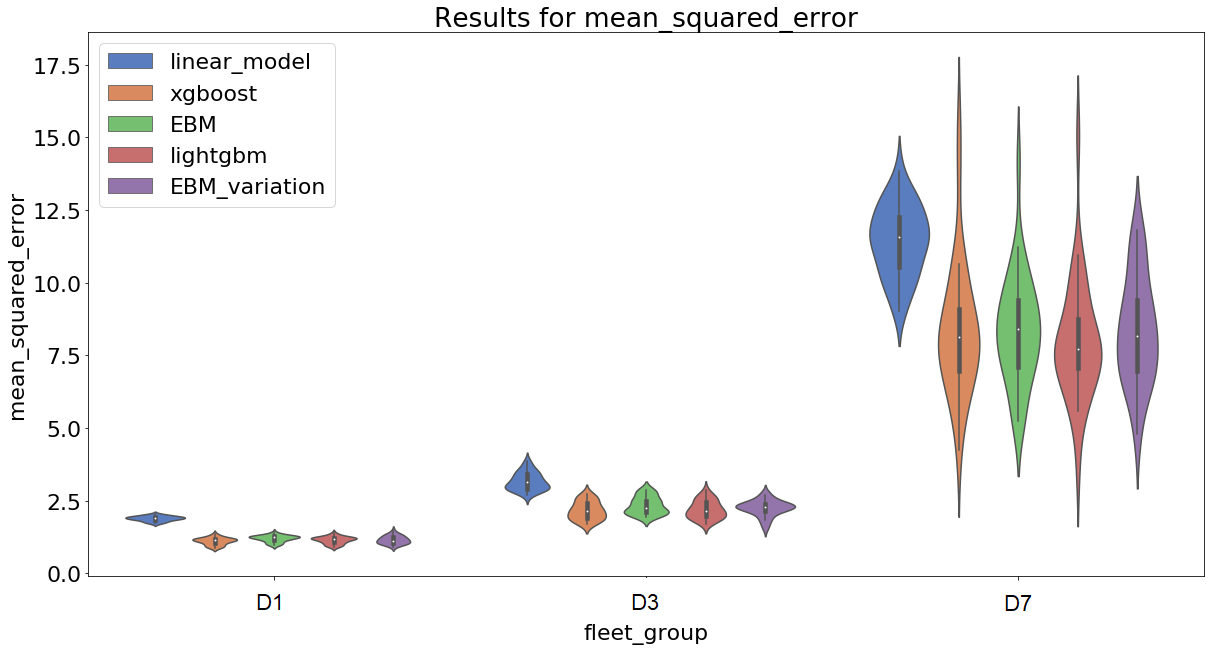
\includegraphics[width=0.8\columnwidth]{figures/chapter6_LucaFleet/model_metrics_mean_squared_error.PNG}
  \end{tabular} 
  \caption{Model metric results for mean squared error. X-axis include the metric value, and Y-axis the three different data sets used.\label{fig:ch6-model-metrics-mean-squared-error}. It shows similar metrics regarding EBM and EBM\_var compared to XGBoost and LightGBM.}
\end{figure}

%\textbf{Analysis of the quality of the model performance metrics}\\
\subsubsection{Analysis of the quality of the model performance metrics}\label{subsubsec:ch6-quality-model-performance}
After the previous analysis, we check the results from \textbf{EBM, EBM\_var, and CGA2M+} over the different data sets in order to see if the results are good enough over the test set (all test set, not only outlier data), and using the raw model predictions (without the business rules).

Regarding adj-R2, even if it's clear that it indicates the proportion of the variance in the target feature that can be predicted using the input features, it is not trivial to define value thresholds to indicate if the model is good or not. It heavily depends on both the context and the units of the target feature \parencite{hair2016primer, hair2013partial}. However, there are some guidelines that may be considered. As a reference, we use the proposal of \parencite{chin1999structural} that mentions the following levels: $0.67$ \textit{substantial}, $0.33$ \textit{moderate} and $0.19$ \textit{weak}.

MAPE, is a metric commonly used for forecasting models. However, it can be also useful for regression tasks \parencite{de2016mean}. Though it is also not direct to define thresholds for MAPE, we use as reference the ones detailed in \parencite{lewis1982industrial}, originally proposed for forecasting models: $<0.1$ \textit{highly accurate}, $[0.1-0.2]$ \textit{good}, $[0.2-0.5]$ \textit{reasonable} and $>0.5$ \textit{inaccurate}.

The metrics over the test set for each ML model used for predicting the fuel consumption over each one of the data sets considered appear in \hyperref[table:ch6-mape-r2-test]{Table} \ref{table:ch6-mape-r2-test}, where we see the mean MAPE over each vehicle in every data set, as well as the adjusted R2 metric for all the predictions in every data set. \textbf{For EBM\_var, we  see that in all data sets the MAPE value is \textit{highly accurate}, with the exceptions of D3, D4 and D9) where is \textit{good}. The same happens with CGA2M+, with the exception of D4, which is \textit{highly accurate} in this case . For Adjusted R2, EBM\_var is always within the \textit{substantial} category, except for the case of D4, where it is \textit{moderate}. The same happens with CGA2M+.}

\begin{table}[h!]
\centering
\resizebox{280pt}{!}{%
\begin{tabular}{@{}llllllll@{}}
\toprule
\textbf{\begin{tabular}[c]{@{}l@{}}Data \\ set\end{tabular}} &
  \textbf{\begin{tabular}[c]{@{}l@{}}MAPE \\ EBM\end{tabular}} &
  \textbf{\begin{tabular}[c]{@{}l@{}}MAPE\\ EBM\_var\end{tabular}} &
  \textbf{\begin{tabular}[c]{@{}l@{}}MAPE\\ CGA2M+\end{tabular}} &
  \textbf{\begin{tabular}[c]{@{}l@{}}Adjst R2\\ EBM\end{tabular}} &
  \textbf{\begin{tabular}[c]{@{}l@{}}Adjst R2\\ EBM\_var\end{tabular}} &
  \textbf{\begin{tabular}[c]{@{}l@{}}Adjst R2\\ CGA2M+\end{tabular}} \\ \midrule
\textbf{D1} 
& \cellcolor{green!25}0.08 
& \cellcolor{green!25}0.08 
& \cellcolor{green!25}0.08 
& \cellcolor{green!25}0.77 
& \cellcolor{green!25}0.8  
& \cellcolor{green!25}0.79 \\
\textbf{D2} 
& \cellcolor{green!25}0.09 
& \cellcolor{green!25}0.08 
& \cellcolor{green!25}0.08 
& \cellcolor{yellow!25}0.66 
& \cellcolor{green!25}0.84 
& \cellcolor{green!25}0.85 \\
\textbf{D3} 
& \cellcolor{yellow!25}0.13 
& \cellcolor{yellow!25}0.11 
& \cellcolor{yellow!25}0.14 
& \cellcolor{green!25}0.94
& \cellcolor{green!25}0.96 
& \cellcolor{green!25}0.92 \\
\textbf{D4} 
& \cellcolor{green!25}0.09 
& \cellcolor{yellow!25}0.10 
& \cellcolor{green!25}0.09 
& \cellcolor{yellow!25}0.61 
& \cellcolor{yellow!25}0.64 
& \cellcolor{yellow!25}0.61 \\
\textbf{D5} 
& \cellcolor{green!25}0.09 
& \cellcolor{green!25}0.08 
& \cellcolor{green!25}0.08 
& \cellcolor{yellow!25}0.66 
& \cellcolor{green!25}0.72 
& \cellcolor{green!25}0.72 \\
\textbf{D6} 
& \cellcolor{green!25}0.09 
& \cellcolor{green!25}0.07 
& \cellcolor{green!25}0.08 
& \cellcolor{green!25}0.85 
& \cellcolor{green!25}0.9  
& \cellcolor{green!25}0.86 \\
\textbf{D7} 
& \cellcolor{green!25}0.08 
& \cellcolor{green!25}0.07 
& \cellcolor{green!25}0.09 
& \cellcolor{green!25}0.8  
& \cellcolor{green!25}0.83 
& \cellcolor{green!25}0.82 \\
\textbf{D8} 
& \cellcolor{green!25}0.08 
& \cellcolor{green!25}0.08 
& \cellcolor{green!25}0.06 
& \cellcolor{yellow!25}0.63 
& \cellcolor{green!25}0.69 
& \cellcolor{green!25}0.67 \\
\textbf{D9} 
& \cellcolor{yellow!25}0.15
& \cellcolor{yellow!25}0.15 
& \cellcolor{yellow!25}0.17 
& \cellcolor{green!25}0.85 
& \cellcolor{green!25}0.84 
& \cellcolor{green!25}0.81 \\ \bottomrule
\end{tabular}%
}
\caption{MAPE and Adjusted R2 over the test set for each ML model and for each data set. Green cells indicate metrics that are inside the best category, while yellow indicate second best.}
\label{table:ch6-mape-r2-test}
\end{table}

\subsection{Prior domain knowledge evaluation}\label{subsec:ch6-eval-xai-apriori}
Now, we focus on analysing whether our proposal (for the case of EBM\_var) yields explanations that are aligned to prior domain knowledge or not. Since this evaluation is carried out over the explanations, we only focus on the vehicles that have fuel consumption anomalies (in all of them, not only in the test set). We also focus on the 4 months of data where the winter period is included (in order to be able to assess the impact of the ambient temperature). Using the models, we get the explanations for each vehicle-date for that period of data, and we aggregate the median feature impact values per subcategory and per vehicle fleet. The median results regardless of the fleet appear in \hyperref[figure:ch6-BoxPlotVehicleFuelImpact]{Figure} \ref{figure:ch6-BoxPlotVehicleFuelImpact}, and the median results considering fleet and including the limits from the SOTA appear in \hyperref[figure:ch6-FeatureImpactperDataset]{Figure} \ref{figure:ch6-FeatureImpactperDataset}. For the analyses, we have considered only vehicles that have a median MAPE over the test set of "Good forecasting" or better unless otherwise indicated (following the criteria from previous subsection).

The categories that we study are "Auxilary Systems" (for all the features that imply an additional electrical energy consumption), "Driving Behaviour" (driver-related features), "Road Conditions", "Vehicle Conditions" and "Weather Conditions". Regarding "Vehicle Conditions", we have included additional variables within the "Other" subcategory with respect to \parencite{zacharof2016review} (e.g. the additional fuel consumption when the DEF level is low), so it does not match the ones covered in that review. Because of that, this subcategory will not be used for checking the hypotheses already mentioned. We do not consider "Rain" subcategory, since the review only provides one reference value.

\begin{figure}[h!]
\centering
 \begin{tabular}{c@{\qquad}c@{\qquad}c}
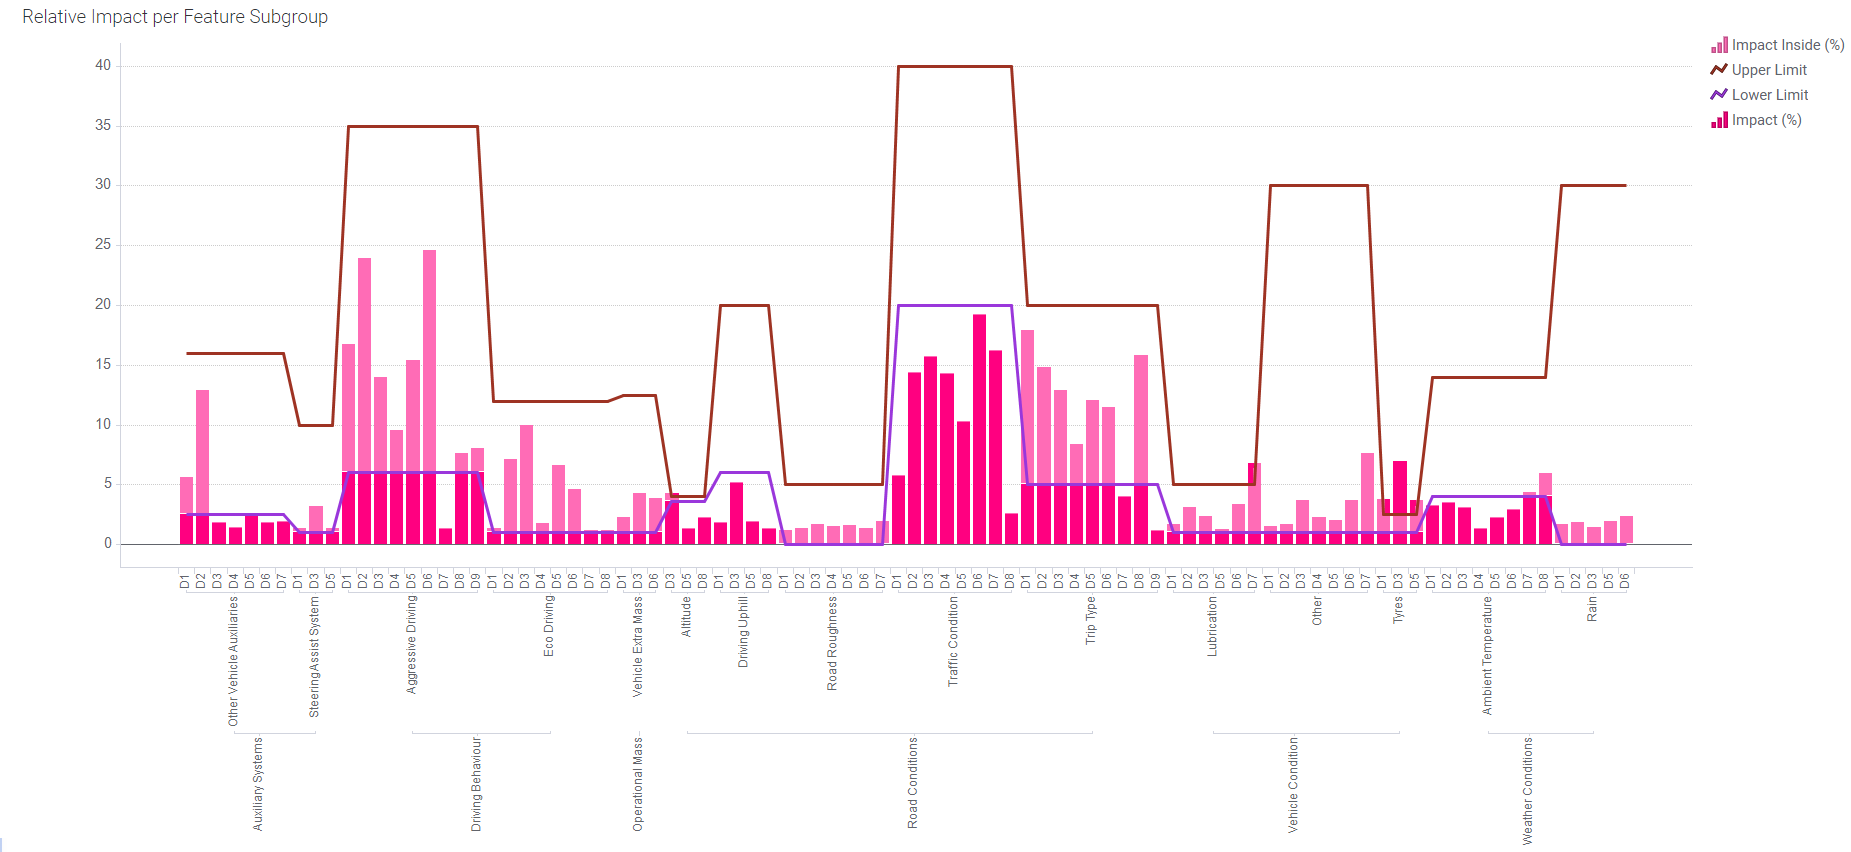
\includegraphics[width=0.95 \columnwidth]{figures/chapter6_LucaFleet/FeatureImpactperDataset.PNG}
  \end{tabular} 
  \caption{Median feature impact per Category-Subcategory-Fleet and the corresponding limits from the literature \parencite{zacharof2016review}  \label{figure:ch6-FeatureImpactperDataset}}
\end{figure}

Thus, in \hyperref[figure:ch6-FeatureImpactperDataset]{Figure} \ref{figure:ch6-FeatureImpactperDataset}, we see that, for 46 combinations, out of the 78 (without the Subcategories of "Other" and "Rain", as mentioned before), the feature relevance is within the limits from the SOTA. The remaining 32 that are not within the limits is because they are either lower than the minimum value used, or higher (for all the three data sets where tyres are relevant, and Lubrication for D7). "Aggressive Driving", "Eco-Driving", "Trip Type" and "Road Roughness" are the Subcategories that are both common in all data sets while having an aggregated feature impact that is within the literature limits. Others, such as "Steering Assist Systems" and "Vehicle Extra Mass" are also fully within the limits, but they are features that are relevant only for some data sets.

With \hyperref[figure:ch6-BoxPlotVehicleFuelImpact]{Figure} \ref{figure:ch6-BoxPlotVehicleFuelImpact} we see the individual impact per vehicle and date, for all the data sets considered together. As the figure shows, "Other Vehicle Auxiliaries", "Steering Assist Systems", "Aggressive Driving", "Eco Driving", "Vehicle Extra Mass", "Road Roughness", "Trip Type, and "Lubrication" have a median value per vehicle-date that is within the limits from the SOTA. For some Subcategories, such as "Steering Assist Systems", "Vehicle Extra Mass", and "Road Roughness", the upper whisker value from the boxplot is also within the SOTA limits. Other subgroups where the median value was not within the limit (because it was below the lower limit), the upper whisker is within the SOTA limits. This is the case of "Ambient Temperature", "Traffic Condition" and "Driving Uphill".
We see, however, that even though the impact per Subcategory normally does not exceed the upper values reported, there are data points where the impact is above the thresholds from the literature. 
%ch:sota
%table:sota-factors-table

\begin{figure}[h!]
\centering
 \begin{tabular}{c@{\qquad}c@{\qquad}c}
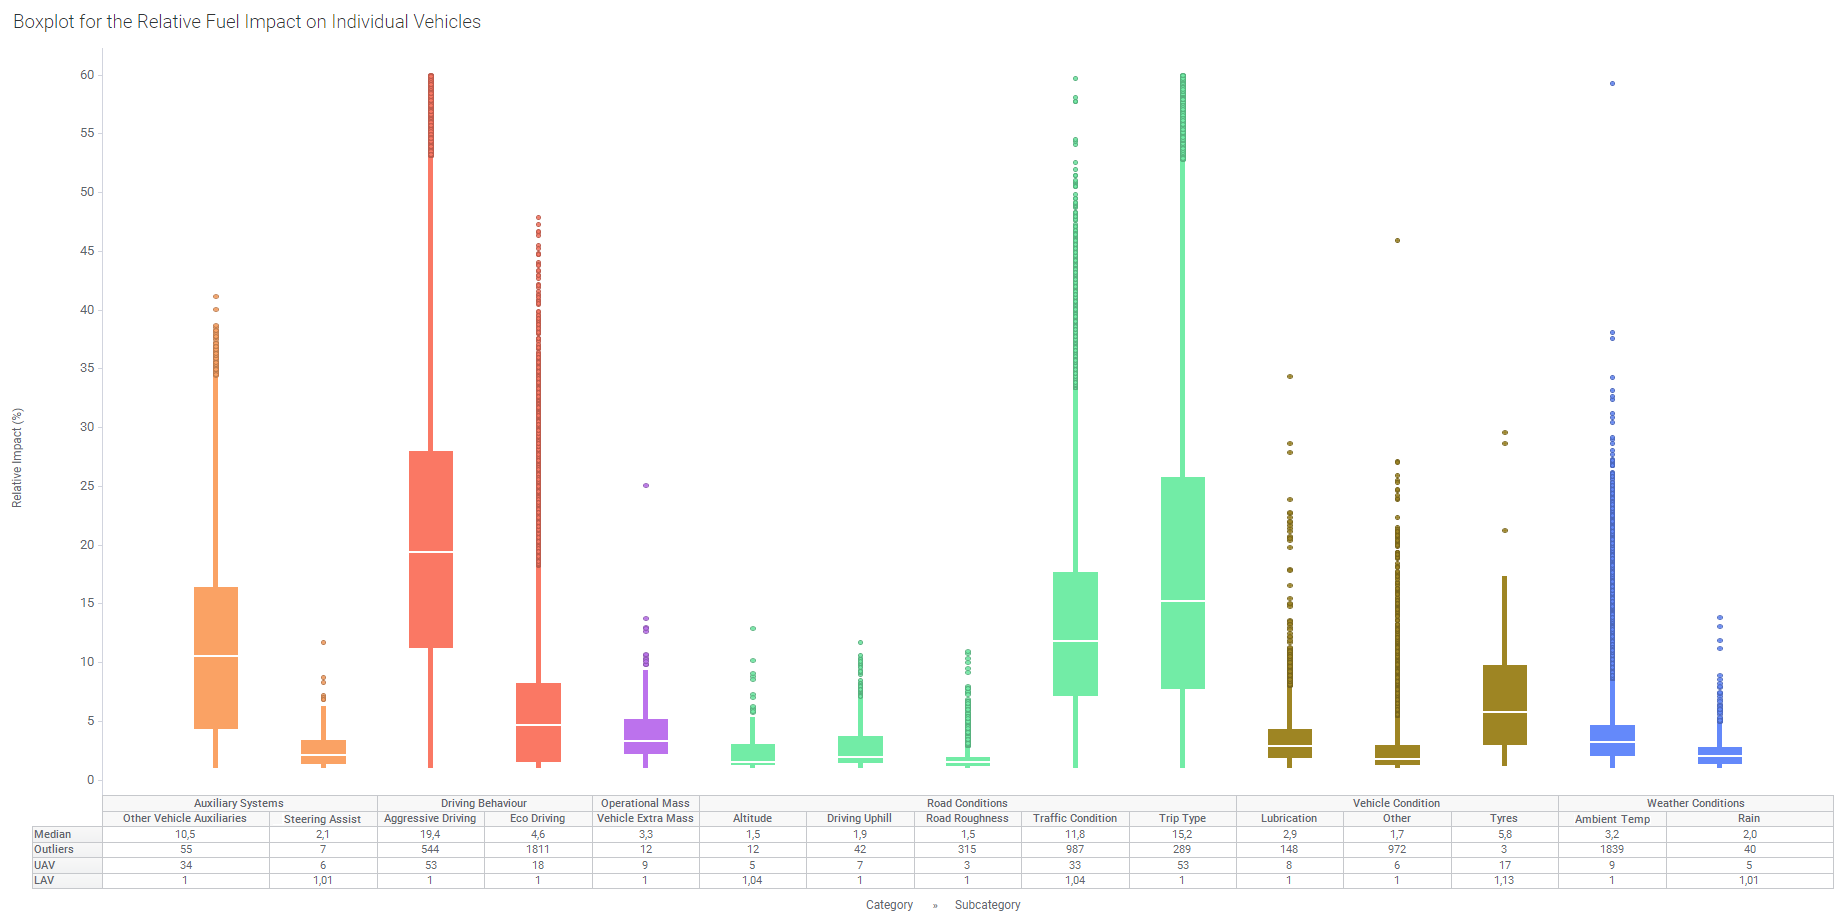
\includegraphics[width=0.9 \columnwidth]{figures/chapter6_LucaFleet/BoxPlotImpact.PNG}
  \end{tabular} 
  \captionsetup{justification=centering}
  \caption{Subcategory fuel impact per vehicle-date.\label{figure:ch6-BoxPlotVehicleFuelImpact}}
\end{figure}

With that, \textbf{we validate this analysis for the 74 out of the 78 combinations of subcategories-data sets since they have an influence in the fuel consumption because the relative impact is always below the maximum SOTA values, and in some cases, its even between them}. The exceptions are all the cases of the impact due to features associated to the "Tyres" subcategories, and "Lubrication" for D7.


\subsection{XAI evaluation}\label{subsec:ch6-eval-xai}
For this evaluation we assess the XAI metrics over the outlier explanations in terms of representativeness, precision, stability, contrastiveness and consistency with apriori beliefs, introduced in \hyperref[subsec:ch6-metrics]{Subsection} \ref{subsec:ch6-metrics}. For precision and stability, we use the outliers within the test set only, since they are metrics related to the prediction output itself. For the remaining XAI metrics, we use all the outlier data points.
The results are displayed in \hyperref[table:annex-xai-metrics-contrast]{Table} \ref{table:annex-xai-metrics-contrast}, showing the Kruskal-Wallis hypothesis contrast test \parencite{kruskal1952use} comparing the results between the three interpretable methods. The table shows the metric comparison in terms of the metric mean value, using the same date set-vehicle-date series when carrying out the comparison for a metric between two algorithms. The study is carried out over all the outlier data available (since we want to compare the explanation quality). We first compare the results without using the monotonicity filter (expect for obtaining \textit{per\_mon} metric), and then we compare the results using it.

Considering \textbf{representativeness} metrics, we analyse both the number of features used by the models within the explanations for a particular vehicle-date (\textit{n\_features}), and the percentage of fuel covered by the features used in the explanations (\textit{rel\_importance}). For all the combinations of algorithms-data set-metric we see statistically significant differences. Regarding \textit{n\_features}, we see that on Large and Medium data sets, EBM\_var is the algorithm that uses more features in the final explanations. However, for Small data sets, the one that uses more features is CGA2M+. This makes sense, since the benefits of EBM\_var only appear with a fleet that has a medium/large amount of vehicle models. For \textit{rel\_importance}, the results are also logical: it can be expected that \textit{rel\_importance} is higher in EBM than in EBM\_var since the former uses less features (meaning that EBM\_var is able to include more features, but that do not have a significant impact compared to the rest). 

For the \textbf{precision} XAI metric, we assess the predictive power of the explanations, which include the business rules for generating them, as opposed to the model's evaluation carried out before, which accounted only for the prediction itself, regardless of the explanations. On every type of data set, EBM and EBM\_var provide similar results. Compared to CGA2M+ the results are also similar, except for Medium data sets, where both EBM and EBM\_var outperform CGA2M+. We can also analyze the MAPE value of the metrics by themselves over the outliers and with the final explanations. Considering the MAPE thresholds defined previously, we see that on Large and Medium data sets, the predictive power with the final explanations and focusing only on the outliers (and only from the test set), is \textit{reasonable}, being very close to \textit{good} category. On Small data sets, the results are on the borderline between \textit{reasonable} and \textit{inaccurate}. This is related to the loss of predictive power due to the business rules constraints, as well as the relatively small data set considered (since we are only focusing on the outliers on the test set). Thus, even though the results are not necessary bad, what is interesting is that for some cases, the results are still accurate even after applying the business rules.

With \textbf{stability} metric, we do not see statistically significant differences in Large data sets. In Medium data sets, EBM is the algorithm with less stability error, while in Small data sets the best results are achieved by CGA2M+. With all that, we see that when there is enough data points, the stability error tends to be the same in all the models, and even though in those cases, generally EBM is the algorithm that achieves a lower stability error, having then the best results.

Regarding \textbf{contrastiveness}, there are many cases where the differences are statistically significant. In Large and Medium data sets, EBM\_var yields the best results in terms of percentage of fuel variation from the daily recommendations (\textit{per\_var}). In Small data sets, the best results are provided by CGA2M+. For the percentage of data points that will be below the anomaly threshold (\textit{per\_below}), we see similar results, with EBM\_var having the greatest reduction percentage for Large and Medium data sets, and CGA2M+ for Small ones. This is logical; when there are enough data points, the constraints on the explanations from the point of view of EBM\_var do not have a significant penalization, thus, the model is able to cover significant information with the explanations. However, for smaller data sets, imposing the constraints during the learning (CGA2M+) yields richer explanations.

In the case of \textbf{apriori beliefs}, we see the degree of monotonicity for EBM and EBM\_var, compared to the perfect degree of monotonicity from CGA2M+. We see that in both cases the degree of monotonicity is significantly lower than the perfect score, and that EBM is significantly more stable than EBM\_var in terms of this metric.

Thus, this first analysis, showed that \textbf{in Large and Medium data sets, the results from EBM\_var are solid, achieving good results on most of the metrics}. This indicates that when there are enough data points, the business rules and its associated constraints can be applied over this model, and still provide good results. The model is also able to use significantly more features and cover more fuel than either EBM or CGA2M+. \textbf{For Small data sets, the results are more contested}. It is true that EBM\_var is similar on several metrics to both EBM and CGA2M+, but \textbf{in some other cases, CGA2M+ provides better results}.

Continuing with the measurements of apriori beliefs, we check the MAPE value of the new average fuel consumption for each vehicle-date after from the final recommendations, \textbf{compared to the catalog fuel consumption} for the same make, model, year, fuel type and route type. For this analysis we only use D1, since it is the largest fleet and because we know exactly the vehicle models and its associated catalog fuel consumption reference. Results appear in \hyperref[table:ch6-comparison-fuel-reference]{Table} \ref{table:ch6-comparison-fuel-reference}, with MAPE 1 corresponding to the median MAPE versus the catalog fuel, MAPE 2 corresponds to the median MAPE versus the median fuel inlier vehicles, and MAPE 3 is the same as MAPE 2 but considering only explanations for outlier vehicles. The table also indicates the percentage of data points with a MAPE 1 below different threshold values (0.5, 0.2, 0.1). It also indicates the percentage of instances with a new fuel consumption below the catalog reference. We see that the results are similar for the three models, with CGA2M+ being better for the percentage of vehicles below the catalog fuel reference. 

\begin{table}[h!]
\centering
\resizebox{200pt}{!}{%
\begin{tabular}{@{}llllllll@{}}
  \textbf{Method} &
  \rot{\textbf{MAPE 1}} &
  \rot{\textbf{MAPE 2}} &
  \rot{\textbf{MAPE 3}} &
  \rot{\textbf{\% MAPE 1 \textless 0.5}} &
  \rot{\textbf{\% MAPE 1 \textless 0.2}} &
  \rot{\textbf{\% MAPE 1 \textless 0.1}} &
  \rot{\textbf{\% Below Catalog}} \\ \midrule
EBM      & 0.14 & 0.14 & 0.14 & 94.2 & 64.2 & 36.8 & 3.3 \\
EBM\_var & 0.15 & 0.14 & 0.14 & 93.2 & 62.6 & 35.6 & 3   \\
CGA2M+    & 0.14 & 0.13 & 0.14 & 94.4 & 63.9 & 36.7 & 2.6 \\ \bottomrule
\end{tabular}%
}
\caption{Different MAPE metrics for each of the models versus the catalog fuel consumption (MAPE 1), the median inliers (MAPE 2), or considering only the vehicles with outlier fuel consumption versus the inliers (MAPE 3).}
\label{table:ch6-comparison-fuel-reference}
\end{table}

\hyperref[fig:ch6-FuelReductionPerModel]{Figure} \ref{fig:ch6-FuelReductionPerModel} shows the average potential fuel reduction with each of the algorithms over every vehicle model and route type, considering the case of D1. We see how CGA2M+ generally provides fuel reductions that are more conservative than the other two methods. The advantage is that there are no cases where the new fuel consumption is below the catalog fuel reference. Comparing EBM\_var with EBM, we see that the first method generally provides recommendations that decrease more the fuel consumption.
This can be seen in \hyperref[fig:ch6-FuelImpactperFeature]{Figure} \ref{fig:ch6-FuelImpactperFeature} and \hyperref[fig:ch6-PairplotComparison]{Figure} \ref{fig:ch6-PairplotComparison}. In \hyperref[fig:ch6-FuelImpactperFeature]{Figure} \ref{fig:ch6-FuelImpactperFeature} we see the daily mean feature fuel impact (in L) for D1 comparing the different models. There, we see how some of the features that have a very high impact on fuel consumption for EBM and EBM\_var do not appear with CGA2M+ after retrieving the explanations and applying the business rules filters. This is the case of "rpm\_high". 

\begin{figure}
  \centering
  \begin{tabular}{c@{\qquad}c@{\qquad}c}
  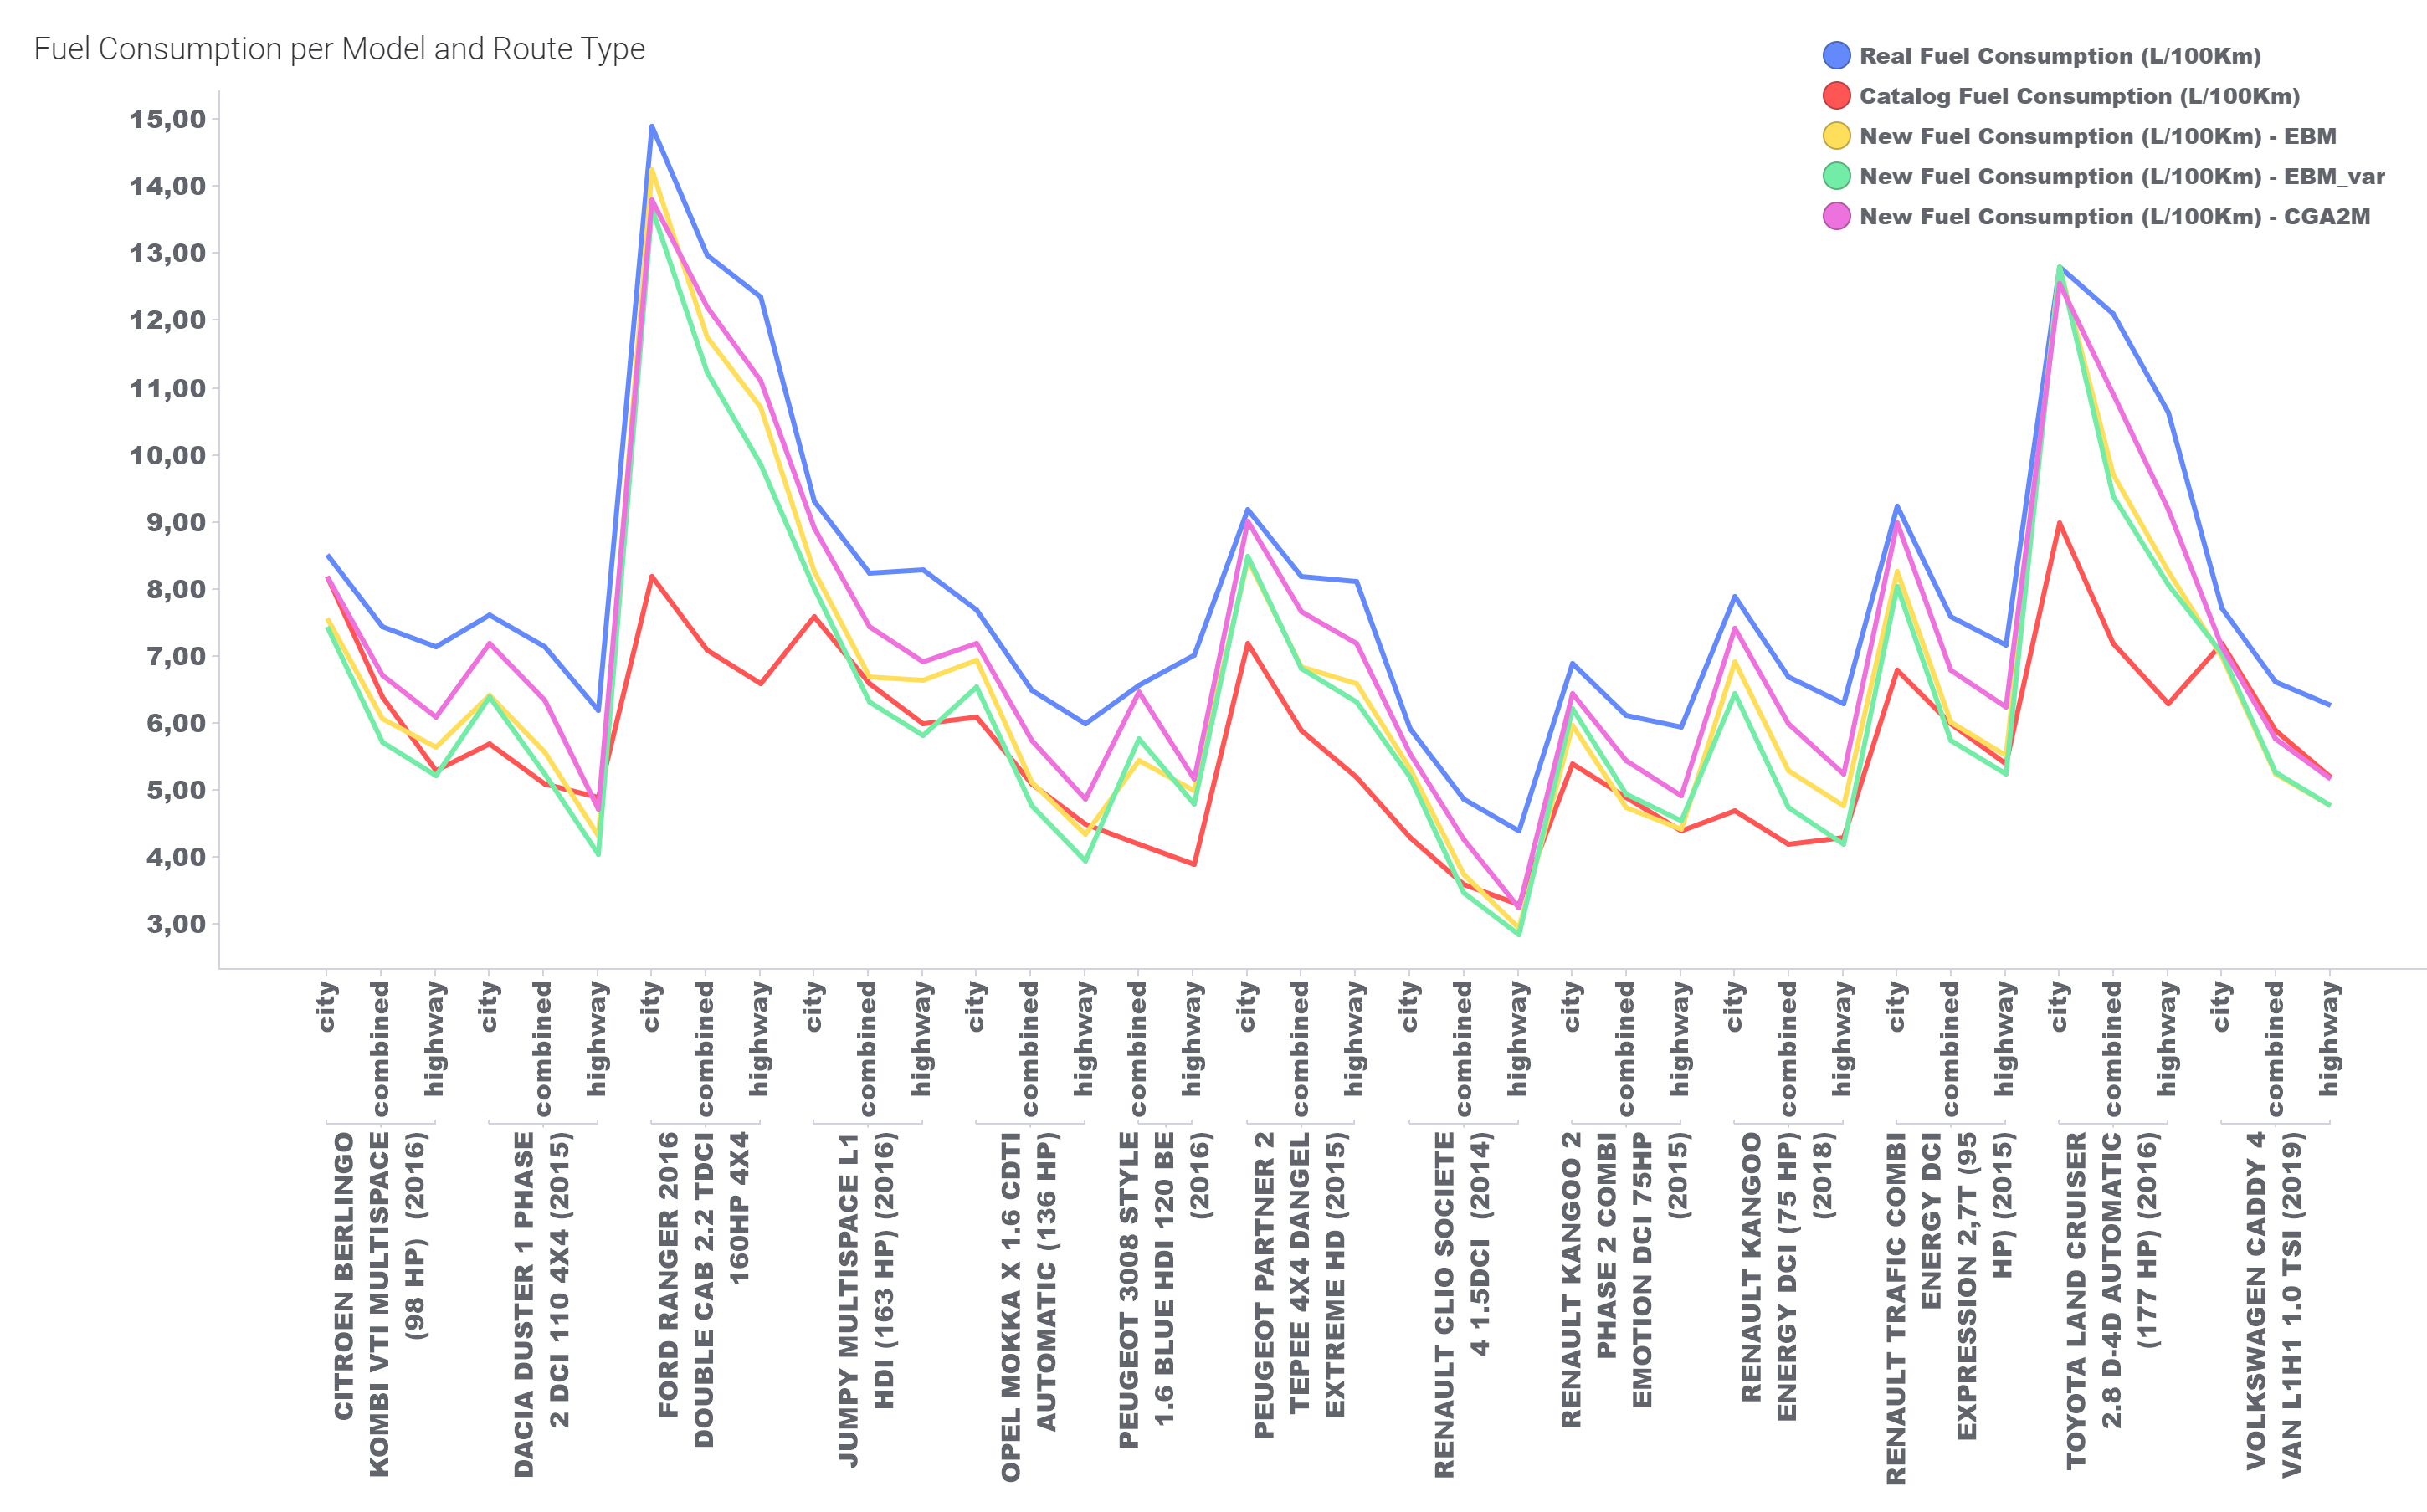
\includegraphics[width=420pt]{figures/chapter6_LucaFleet/FuelReductionPerModel.PNG}
  \end{tabular} 
  \caption{Comparison of the potential fuel reduction per vehicle model and route type for D1. The comparison includes the three algorithms with respect to both the real fuel consumption and the catalog reference.\label{fig:ch6-FuelReductionPerModel}}

  \begin{tabular}{c@{\qquad}c@{\qquad}c}
  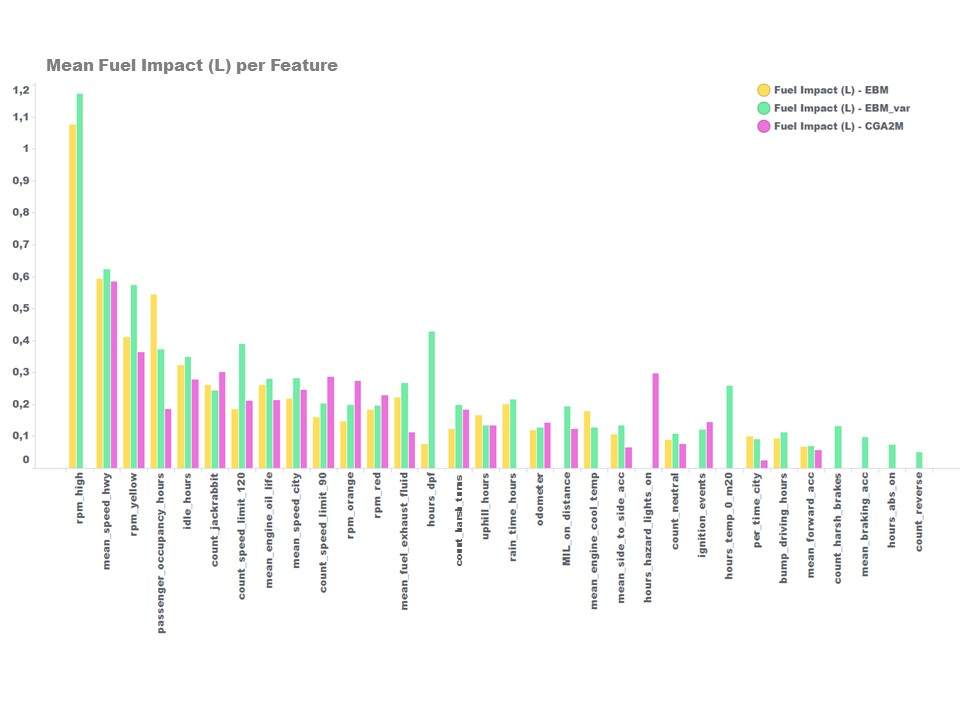
\includegraphics[width=410pt]{figures/chapter6_LucaFleet/FuelImpactperFeature.jpg}
  \end{tabular} 
  \caption{Daily mean feature fuel impact (in L) for D1, comparing the different models. Features shown appear at least within 100 vehicle-dates combinations.\label{fig:ch6-FuelImpactperFeature}}
\end{figure}

Focusing on some vehicle models and some of the features with higher impact, we see in \hyperref[fig:ch6-PairplotComparison]{Figure} \ref{fig:ch6-PairplotComparison} the relationship between feature relevance and feature values, using the data set D1. It shows how in many cases, the CGA2M+ curve is below the ones from the other methods, since it needs to be monotonic. We also see how EBM and EBM\_var are able to extract relationships that are almost monotonic (e.g. for "Trip Kms" or "Mean Speed Hwy"), while the relationships in other cases are clearly non monotonic (e.g. "Hours Raining" or "Count Events Speed $>$ 120 Km/h). This plot shows the values for EBM and EBM\_var before applying the monotonicity filtering.

\begin{figure*}
\centering
\begin{tabular}{c@{\qquad}c@{\qquad}c}
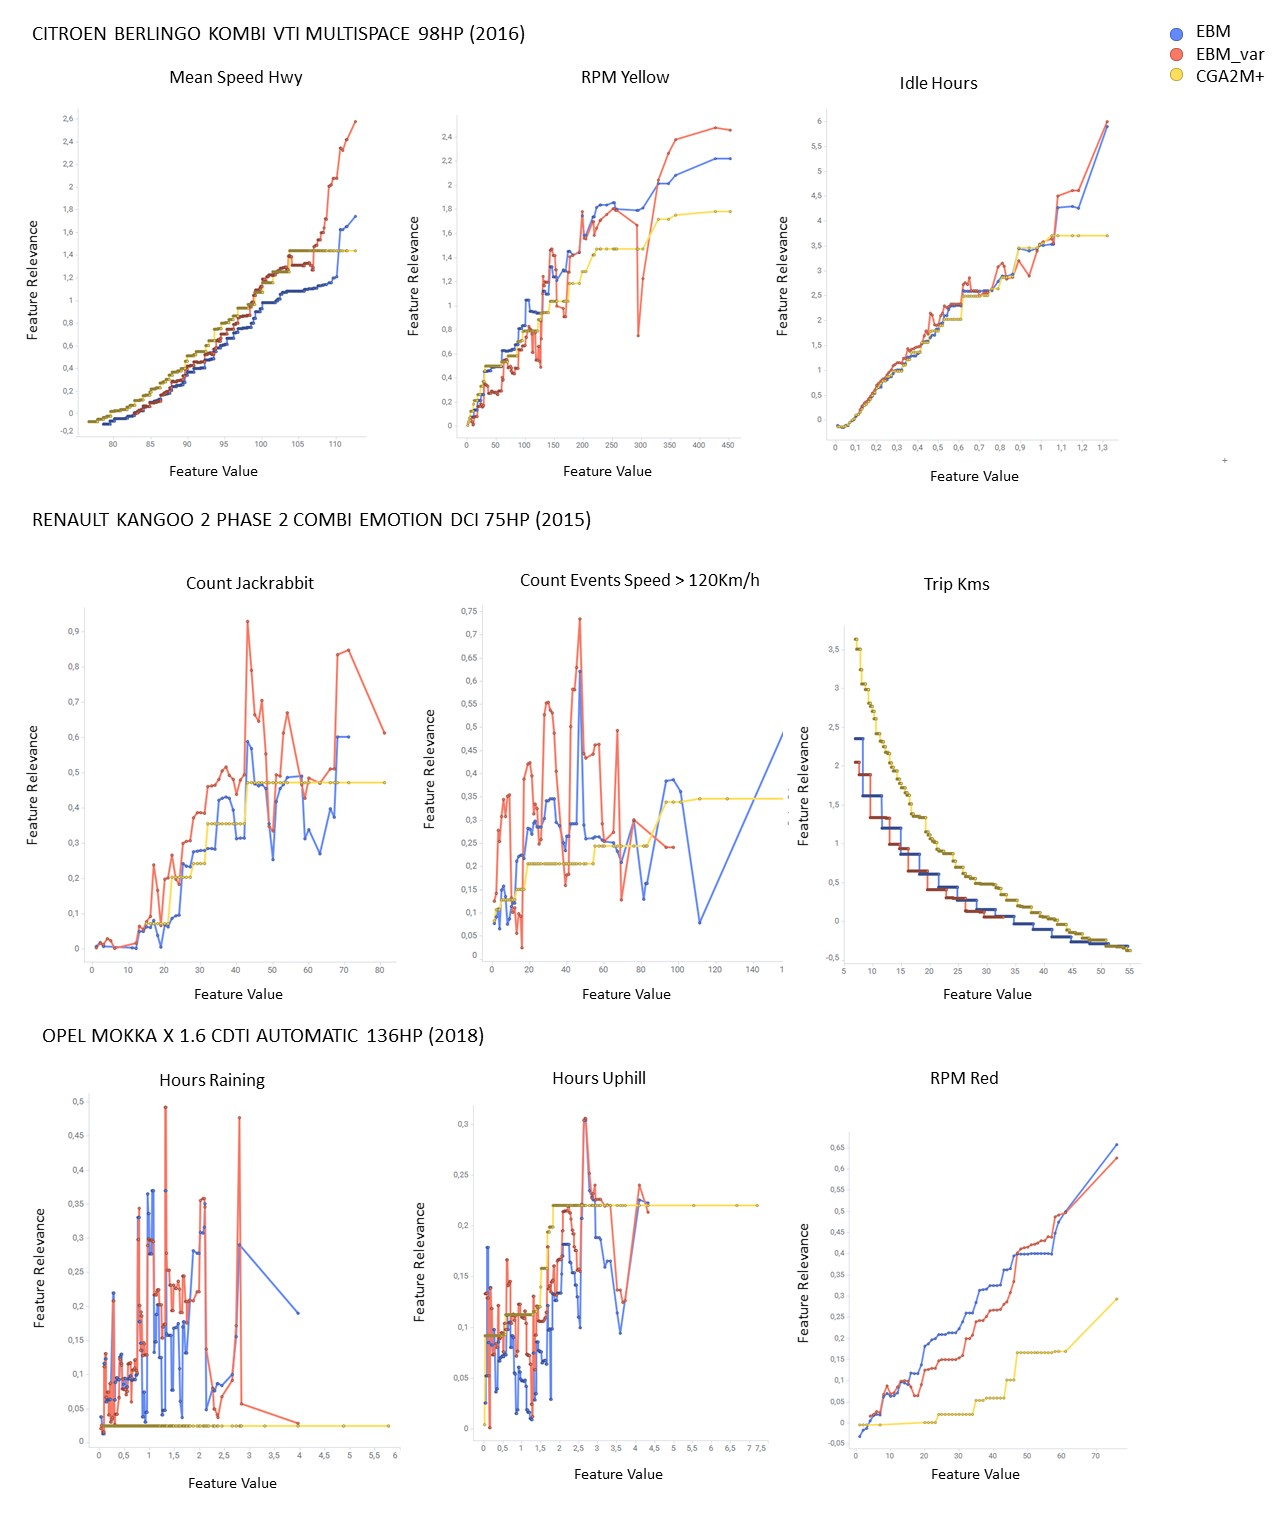
\includegraphics[width=\textwidth]{figures/chapter6_LucaFleet/PairplotComparison.jpg}
  \end{tabular} 
  \caption{Pairplot with the relevance-values for several features considering data points for some vehicle's models only, and using the data set of D1 (without applying the monotonicity filtering in EBM and EBM\_var).\label{fig:ch6-PairplotComparison}}
\end{figure*}

Extending the analysis to the other data sets, and focusing on the outliers only, we get the results shown in \hyperref[table:ch6-Fuel-Saved-Explained]{Table} \ref{table:ch6-Fuel-Saved-Explained}. We see how CGA2M+ still covers less fuel (in L) than EBM\_var for all data sets except for the smallest ones (D8 and D9). \textbf{On average, the fuel reduced among the largest data sets by EBM\_var final explanations is over 38\%, and over 29\% with CGA2M+.}

However, applying the monotonicity constraints over EBM and EBM\_var leads to a scenario where CGA2M+ covers more fuel than either EBM or EBM\_var, except for D1. This shows that if there is a need to \textbf{ensure the monotonicity of the feature explanation output}, and specially if the fleet size is not high enough, it is \textbf{better to impose it during the model learning} (CGA2M+), than applying it post hoc (EBM or EBM\_var). 

% TODO: Meter aqui la ultima comparativa con la tabla monotonicity filter
This last aspect is clearly seen in \hyperref[table:annex-xai-metrics-contrast-mono]{Table} \ref{table:annex-xai-metrics-contrast-mono}, where we show the XAI metrics after applying the monotonicity filter in EBM and EBM\_var (and with respect to the same CGA2M+ metric values). On general terms, CGA2M+ provides better results in all fleet sizes (though for \textit{precision} and \textit{contrastiveness} metrics the results are more similar). We also see that the filter penalizes more EBM\_var than EBM (since the monotonicity degree is higher in EBM). This points to two possible scenarios. When there is no need to ensure the monotonicity degree at every feature level (e.g., when the explanations are at a global level for profiles like fleet managers), EBM\_var is a good choice. However, when there is a need for ensuring the monotonicity within the individual explanations (e.g., for fleet operators), it is better to ensure it during the model's learning (CGA2M+), than afterwards. 

\begin{table}[h!]
\centering
\resizebox{420pt}{!}{%
\begin{tabular}{@{}lllllllll@{}}
\toprule
\textbf{\begin{tabular}[c]{@{}l@{}}Data \\ set\end{tabular}} & \textbf{Method} & \textbf{N points} & \textbf{\begin{tabular}[c]{@{}l@{}}Points\\ Expl. (\%)\end{tabular}} & \textbf{\begin{tabular}[c]{@{}l@{}}Fuel\\ Used (L)\end{tabular}} & \textbf{\begin{tabular}[c]{@{}l@{}}Fuel\\ Saved (L)\end{tabular}} & \textbf{\begin{tabular}[c]{@{}l@{}}Fuel\\ Saved (\%)\end{tabular}} & \textbf{\begin{tabular}[c]{@{}l@{}}Fuel Expl.\\ Monotonic (\%)\end{tabular}} & \textbf{\begin{tabular}[c]{@{}l@{}}Fuel Saved\\ Monotonic (\%)\end{tabular}} \\ \midrule
D1 & EBM & 5770 & 74 & 28599 & 6200 & 22 & 70 & 18 \\
D1 & EBM\_var & 5770 & 74 & 28599 & 6925 & 24 & 68 & 16 \\
D1 & monoGAM & 5770 & 70 & 28599 & 4629 & 16 & 70 & 16 \\
D2 & EBM & 1809 & 99 & 23139 & 10005 & 43 & 99 & 37 \\
D2 & EBM\_var & 1809 & 99 & 23139 & 11986 & 52 & 97 & 38 \\
D2 & monoGAM & 1809 & 99 & 23139 & 9710 & 42 & 99 & 42 \\
D3 & EBM & 10475 & 61 & 260152 & 36319 & 14 & 56 & 5 \\
D3 & EBM\_var & 10475 & 61 & 260152 & 46135 & 18 & 56 & 7 \\
D3 & monoGAM & 10475 & 60 & 260152 & 40853 & 16 & 60 & 16 \\
D4 & EBM & 1915 & 65 & 14301 & 1932 & 14 & 58 & 7 \\
D4 & EBM\_var & 1915 & 71 & 14301 & 2622 & 18 & 62 & 10 \\
D4 & monoGAM & 1915 & 69 & 14301 & 2175 & 15 & 69 & 15 \\
D5 & EBM & 724 & 43 & 6816 & 801 & 12 & 42 & 10 \\
D5 & EBM\_var & 724 & 43 & 6816 & 936 & 14 & 43 & 11 \\
D5 & monoGAM & 724 & 42 & 6816 & 763 & 11 & 42 & 11 \\
D6 & EBM & 2002 & 96 & 11157 & 3386 & 30 & 91 & 18 \\
D6 & EBM\_var & 2002 & 98 & 11157 & 4545 & 41 & 93 & 22 \\
D6 & monoGAM & 2002 & 95 & 11157 & 4047 & 36 & 95 & 36 \\
D7 & EBM & 942 & 58 & 41437 & 5995 & 14 & 48 & 8 \\
D7 & EBM\_var & 942 & 57 & 41437 & 6066 & 15 & 41 & 8 \\
D7 & monoGAM & 942 & 21 & 41437 & 4373 & 11 & 21 & 11 \\
D8 & EBM & 349 & 82 & 3164 & 333 & 11 & 69 & 4 \\
D8 & EBM\_var & 349 & 82 & 3164 & 368 & 12 & 65 & 4 \\
D8 & monoGAM & 349 & 92 & 3164 & 1144 & 36 & 92 & 36 \\
D9 & EBM & 10 & 100 & 471 & 44 & 9 & 80 & 3 \\
D9 & EBM\_var & 10 & 100 & 471 & 37 & 8 & 60 & 2 \\
D9 & monoGAM & 10 & 50 & 471 & 70 & 15 & 50 & 15 \\ \bottomrule
\end{tabular}%
}
\caption{Vehicle-dates (N data points) with anomalous fuel consumption explained by the different XAI models on the different fleets, together with the potential fuel saved (L and \%) with the recommendations.}
\label{table:ch6-Fuel-Saved-Explained}
\end{table}

\newpage
\section{Conclusion}\label{sec:ch6-conclusion}
We have proposed a complete process for explainable unsupervised anomaly detection in the fuel consumption of the vehicles of a fleet. Anomalies are explained using Explainable Artificial Intelligence (XAI) techniques and based on the feature relevance of several features that may impact in the fuel usage. The explanations take into account domain knowledge expressed through business rules and expressed through recommendations that are adjusted depending on two different user profiles that will use them: fleet managers and fleet operators. The process is evaluated using real-world data gathered from telematics devices connected to several industry fleets.

We have also evaluated different possibilities for building a surrogate model that infers the relationships between the input data and the predicted fuel consumption, in order to explain later how anomalous fuel consumption could be reduced. For those surrogate models, we have used Generalized Additive Models with Explainable Boosting Machine (EBM), Constrained Generalized Additive 2 Model with Consideration of Higher-Order Interactions (CGA2M+), and a proposal with a variation over the original EBM algorithm. 

To compare the different surrogate model alternatives, we have performed evaluations regarding model performance (how well the model predicts the target feature), and XAI metrics, that compare the explanations generated in terms of representativeness, fidelity, stability, contrastiveness and consistency with apriori beliefs. 

The evaluations show that all interpretable models yield good results in terms of model performance. For the XAI metrics, particularly for the consistency with apriori beliefs, we see that the three models yield good results by themselves and are able to provide appropriate recommendations over 80\% of the anomalous instances, that could potentially lead to fuel reductions of up to 38\% on average on large fleets. The XAI metrics are also used for comparing the models between them, where we saw that in general, both CGA2M+ and EBM\_var provide similar or better results than EBM, while respectively solving monotonicity problems and considering the vehicle model and route type information for adjusting the explanations.

Along with that, we have verified that the explanations are indeed aligned to prior domain knowledge regarding the factors that impact on vehicle fuel consumption. We have also shown how model performance is acceptable even after applying restrictions in the model for aligning the output to prior domain knowledge. Following this, we have also seen that the model performance is similar to that of unconstrained SOTA blackbox models.

With that, the work presented in this chapter serves for evaluating both \textbf{H1} and \textbf{H2}, described in \hyperref[sec:Hypotheses]{Section} \ref{sec:Hypotheses}. Regarding H1, we have applied an XAI approach for explaining the output of an unsupervised anomaly detection algorithm and we have compared the resulting explanations through XAI-specific metrics. For the case of H2, we have combined those XAI approaches with prior domain knowledge, showing that this does not penalize significantly the model performance, and we have analyzed how the final explanations are aligned to that prior knowledge.
Thus, this chapter offers a complete evaluation of the sub-hypothesis that are beneath the main hypothesis of this thesis.

%\subsection{Potential impact}\label{subsec:ch6-conclusion-potential-impact}
%The previous information showed what variables are impacting on the fuel consumption of individual vehicles, and how much fuel could be reduced by acting upon them through the explanations provided. This information is useful for having a full view over the whole fleet and seeing the extra fuel consumption that it is taking place because of those factors. Even more, we can focus on specially actionable factors, such as driving behaviour, in order to see the impact on the fuel consumption due to the driving style. \hyperref[table:ch6-ExtraFuelPerMonth]{Figure} \ref{table:ch6-ExtraFuelPerMonth} shows the fuel consumption on each of the fleets over the four months considered, together with the extra fuel consumption from driving behaviour, and the extra fuel consumption due to the remaining factors.

%\begin{figure}[h!]
%\centering
% \begin{tabular}{c@{\qquad}c@{\qquad}c}
%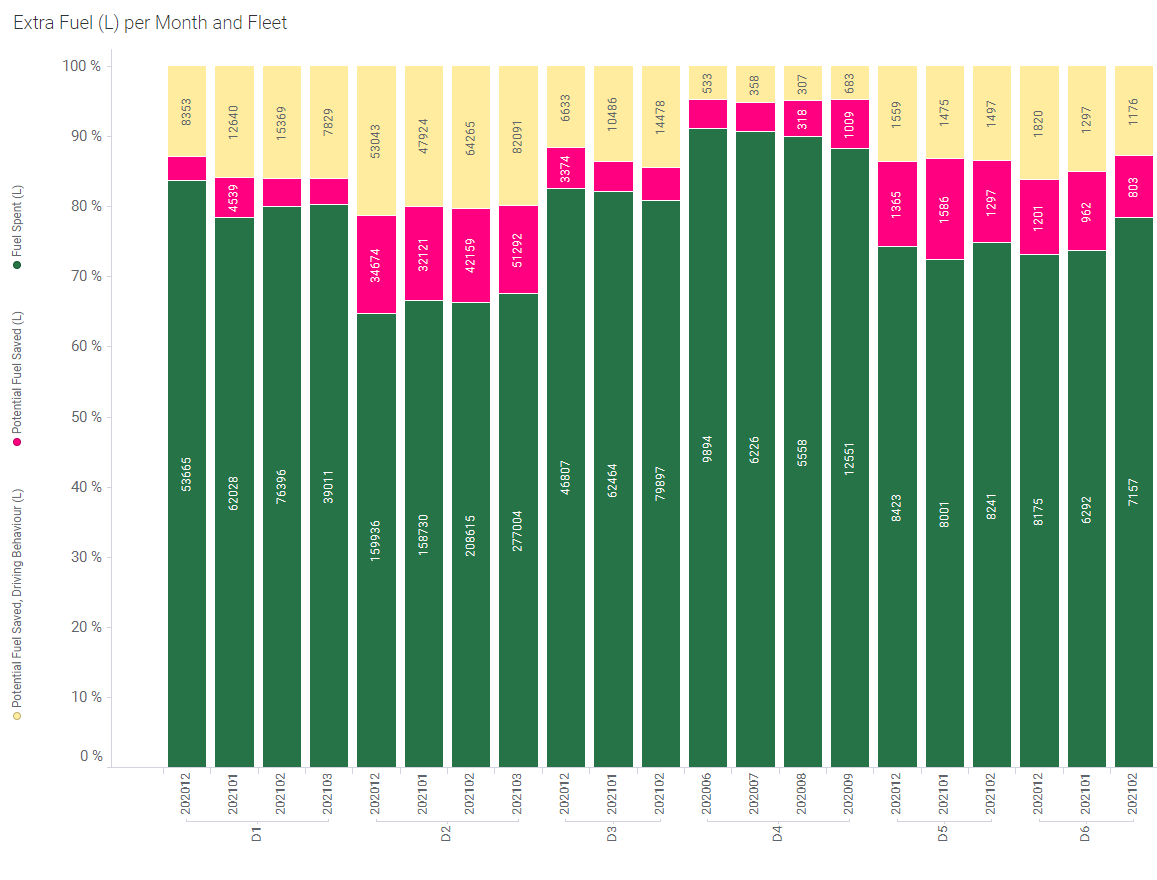
\includegraphics[width=430pt, height=550pt, %keepaspectratio]{figures/chapter6_LucaFleet/ExtraPerMonthFleet.PNG}
%  \end{tabular} 
%  \caption{Monthly fuel consumption (L) for each fleet over the different months, along with the part of that fuel that corresponds to the extra fuel due to driving behaviour, together with the extra fuel from the remaining factors. This is considering both inliers and outliers.  \label{table:ch6-ExtraFuelPerMonth}}
%\end{figure}

%Focusing on D1 (since it is the fleet with more information and that provided better results) and for all data points with extra fuel (even if they are outliers per se), we see that the relative impact of all the features is between 16\% and 22\%, and for driving behaviour only, it is between 13\% and 16\%. Taking as an example the month of February, we see that there are 15546 extra litres spent due to driving behaviour. Reducing it would have a positive impact both in the expenses from the fleet, as well as in the environment. Since the vehicles from D1 are mostly diesel, using the conversion to CO2 from \parencite{DieselLitresTOCo2}, where 2.67633 Kg of CO2 are emitted per liter of diesel spent, the extra CO2 emissions in one month due to driving behaviour is between 22330 and 41085 Kg.
    
    % Final Sections
    %\section{Development}
    
    \vspace{0.3cm}
    \noindent
    \begin{equation}
        W = \sum_{j=1}^{n} \alpha_j U_j(x) + \sum_{j,l=1}^{n} \alpha_{jl} U_j(x) U_l(x) + ... + \alpha_{jl...n} U_j U_l ... U_n
        \label{equation:eq_one}
        \myequations{Test equation one}
    \end{equation}
    \vspace{0.3cm}
    
    \noindent
    \begin{table}[h!]
        \centering
        \begin{tabular}{||c c c c||} 
            \hline
            Col1 & Col2 & Col2 & Col3 \\ [0.5ex] 
            \hline\hline
            1 & 6 & 87837 & 787 \\ 
            \hline
            2 & 7 & 78 & 5415 \\
            \hline
        \end{tabular}
        
        \caption{Test table one}
        \label{table:table_one}
    \end{table}
    
    \noindent
    \begin{figure}[h!]
        \centering
        \includegraphics[scale=0.2]{images/UPM.eps}
        \caption{Test figure one}
        \label{graphic:figure_one}
    \end{figure}


    \subsection{Subdevelopment A}
    
        ...
        
    \subsection{Subdevelopment B}
    
        ...

\newpage
    \chapter{Conclusions and Future Work}\label{ch-conclusions}
This chapter concludes this thesis by including a summary of the contributions to the State of the Art (SOTA), as described in the previous chapters. These contributions address the research problems that are described in \hyperref[chap:3-objetives]{Chapter} \ref{chap:3-objetives}. The main focus of this thesis is studying if Explainable Artificial Intelligence (XAI) can be used for explaining the results of unsupervised learning algorithms for anomaly detection within two real-world contexts. This main hypothesis is divided into two sub-hypotheses. First, analysing that it is possible to indeed use XAI techniques over unsupervised learning algorithms for anomaly detection, and quantitatively measure the quality of explanations through XAI-specific metrics. Second, studying the applicability of XAI and anomaly unsupervised anomaly detection algorithms within real-world industry contexts, where we consider prior domain knowledge for both adjusting the explanations and for measuring their quality against it. 

Following this, \hyperref[sec-conclusions-contrib-1]{Subsection} \ref{sec-conclusions-contrib-1} delves into the contributions related to the first sub-hypothesis, while  \hyperref[sec-conclusions-contrib-2]{Subsection} \ref{sec-conclusions-contrib-2} does it for the second one. \hyperref[sec-conclusions-final]{Subsection} \ref{sec-conclusions-final} provides a final reflection about the potential impact of this work.

\section{Summary of the first contribution and future work}\label{sec-conclusions-contrib-1}
The first contribution of this thesis is related to a core study of the applicability of XAI for explaining unsupervised learning algorithms for anomaly detection, which also includes the usage of XAI-metrics for quantitatively measuring the quality of the explanations in order to compare the results of the XAI techniques among them. 

With that, we have addressed the problem of explaining these models by considering their output the same as the one from a binary classification model. However, some aspects that are different must be taken into account: there is commonly a great data imbalance between the two classes, there is normally a need to explain only one of the classes (outliers) in a counterfactual way, and the explanations must be P@1 within several use cases.

Because of that, even though any post-hoc XAI technique may be theoretically applied, the explanation results may differ, and some techniques may be more suitable than others for this context. In fact, we proposed \textbf{SVM+Prototypes reloaded} as an algorithm that could behave potentially better than others for the specific context of unsupervised anomaly detection. The algorithm serves for generating both post-hoc global and local counterfactual rule-based explanations that are model agnostic, and is a variant from a previous one used in the literature, and comes with two alternative methods for extracting the rules: \textbf{keep} as an approach that keeps all data points in every iteration for extracting the hypercubes, and \textbf{split} as an approach that splits the subspaces with a binary partition scheme until no points from the other class are inside the rules for the target class.

In order to quantitatively measure the results and compare the explanations outputs between the different XAI techniques, we need to use XAI-specific metrics. We used already existing XAI metrics
for measuring their \textit{comprehensibility} and \textit{representativenes} related aspects, and we have also proposed novel algorithms, \textbf{StabilityScore} and \textbf{DiversityScore}, for computing metrics related to the \textit{stability} and \textit{diversity} of the rule explanations. 

With that, we used both our XAI proposals, as well as other SOTA XAI model-agnostic techniques for rule extraction, and compared the explanation results generated over the decision of OneClass Support Vector Machine (OCSVM) models with different kernels and over different data sets. With that, we found out how XAI metrics indeed show that there are significant differences between the XAI techniques.

The results summarized in this subsection serve for checking the first sub-hypothesis, by both mathematically justifying XAI metrics, as well as evaluating them over different data sets in order to quantify explanation differences between rule extraction methods within the context of unsupervised anomaly detection.

All our contributions are included within a framework that standardizes the output of the different rule extraction techniques (by turning them into hypercubes) in order to carry out the evaluation through those metrics. This framework also prunes the rules, eliminating redundant ones. Our framework is available through an open source library.
\\
\\
Nonetheless, our contributions could be enhanced by carrying out additional studies. In the thesis, even though we used model-agnostic posthoc XAI techniques, we only assessed the results from OCSVM models for anomaly detection. Other unsupervised learning, such as IsolationForests \parencite{liu2008isolation}, Local Outlier Factors \parencite{breunig2000lof}, or Deep Learning based models, could be considered. This is also applicable to the XAI techniques themselves, since there are some alternatives, such as G-Rex algorithms \parencite{konig2008g}, not covered within the thesis. The research that lead to our proposed framework for generating and evaluating explanations for anomaly detection could also be continued with supervised ML models, since it is model-agnostic, needing only the input data and the output prediction. Thus, the usefulness of our rule-extraction algorithms and the novel XAI metrics that we proposed can also be studied over other types of ML algorithms and for other use cases beyond anomaly detection.

Within the thesis, we also proposed a simple metric for encapsulating all the individual metrics to simplify the comparisons and analyses. However, beyond computing the metric, we have not conducted an in-depth evaluation of it. Also, there is much room for improvement for finding an optimal function that weights appropriately every term.

%Along with that, rule extraction should also be designed to consider all types of comparisons ($\geq$, $\leq$, $>$ and $<$), and this is something that could also be considered in the cluster-based methods developed.
Along with that, rule extraction should also be designed to consider all types of comparisons ($\geq$, $\leq$, $>$ and $<$).

Finally, even though the metrics are theoretically useful from a quantitative point of view, the analysis should be complemented with user specific studies (considering different user profiles) in order to evaluate their usefulness and their possible alignment with prior domain knowledge.

\section{Summary of the second contribution and future work}\label{sec-conclusions-contrib-2}
The second contribution of this thesis is related to the usage of XAI techniques for explaining unsupervised anomaly detection algorithms within real-world industry contexts, through two use cases, one for communications data and one for the fuel consumption of petrol and diesel vehicles. Since these contexts have an already prior domain knowledge that can be related to the anomaly detection process, we studied both how this knowledge can be used for adjusting the explanations generated, as well as for assessing the quality of the fina explanations against it.

For the use case of communications data, we used a OCSVM for anomaly detection, and we have proposed an algorithm that generates visual and counterfactual explanations over it based on the information of the decision frontier. Our proposal generates visual explanations for a numerical feature with respect to every combination of categorical feature values using the information from the decision frontier of the Machine Learning (ML) algorithm. Along with this, we proposed the usage of a grid search algorithm based on MIES that includes prior domain knowledge, so the explanations generated are aligned with it. With that, the prior domain knowledge is used for choosing only hyperparameter configurations of the anomaly detection model that do not contradict that prior knowledge. We compared the results of this grid search algorithm variation against the results of a grid search that only aims to optimize the results from a pure model performance point of view, and we saw that the results do not have significant statistical differences, indicating that using prior knowledge does not penalize the results.

For the use case of fuel anomalies within vehicle fuel consumption, we have proposed a methodology for explainable unsupervised anomaly detection that detects, explains and provide fuel saving recommendations for those anomalies and for different user profiles, using also prior business domain knowledge. The explanations are feature relevance-based, obtained through surrogate Generalized Additive Models (GAM). This is the core of \textbf{RESYFEX}, a Recommender System (RecSys) that provides actionable recommendations for fuel saving considering two user profiles: fleet managers and fleet operators.

Within this last context, we initially used Explainable Boosting Machine (EBM) as the GAM algorithm, but we detected some limitations with it. First, the feature relevance explanations will be the same for all the vehicles within the fleet. Second, the relationship between feature values and feature relevance may not be monotonic when it should be. For addressing the first problem, we proposed a variation over EBM, \textbf{EBM\_var}, which adjusts the explanations based on the vehicle groups. For the second limitation, we considered two alternatives: using novel models that incorporate learning restrictions for providing monotonic relationships (using Constrained Generalized Additive 2 Model with Consideration of Higher-Order Interactions, CGA2M+, algorithm), or using an algorithm that removes some of the explanations, yielding only the ones that are monotonic. 

To compare the different surrogate model alternatives among themselves, we have performed evaluations regarding model performance (how well the model predicts the target feature), and XAI metrics, that compare the explanations generated in terms of representativeness, fidelity, stability, and contrastiveness.

Complementing this, we also carried out an analysis for ensuring that the explanations provided within this context are aligned to prior domain knowledge regarding the expected impact that those factors have on vehicle fuel consumption. Related to that, we also proposed metrics for measuring the consistency with apriori beliefs.

The results showed that the explanations are indeed aligned to prior domain knowledge regarding the factors that impact on vehicle fuel consumption. We have also shown how model performance is acceptable even after applying restrictions in the model for aligning the output to prior domain knowledge. Following this, we have also seen that the model performance is similar to that of unconstrained SOTA blackbox models. Within the context of XAI metrics, we saw that both CGA2M+ and EBM\_var provide similar or better results than EBM, while respectively solving monotonicity problems and considering the vehicle model and route type information for adjusting the explanations.

With this use case, we checked both sub-hypotheses, described in \hyperref[sec:Hypotheses]{Section} \ref{sec:Hypotheses}. First, we have applied an XAI approach for explaining the output of an unsupervised anomaly detection algorithm and we have compared the resulting explanations through XAI-specific metrics. Second, we have combined those XAI approaches with prior domain knowledge, showing that this does not penalize significantly the model performance, and we have analyzed how the final explanations are aligned to that prior knowledge. This last sub-hypothesis is also checked with the use case regarding communications data by showing how prior domain knowledge can be integrated within the XAI explanations, and this does not harm the predictive power of the model beneath them.
\\
\\
Regarding the future research lines, for the use case of vehicle fuel consumption, we see several areas where our current research can be continued. The first one is regarding the unsupervised algorithm for anomaly detection. Within our proposal, we have used a Box-Plot applied over the fuel consumption of the vehicles of a same group and route type since it directly provides a limit that helps seeing the threshold value that sets apart anomalous fuel consumption and non-anomalous one. It also provides a visual limit that highlights an additional insight for the users since they can see the average fuel split between inliers and outliers. However, there are other unsupervised algorithms that can be used if they can provide that threshold limit.

The second line is regarding the XAI metric usage. The literature proposes other aspects that can be measured in terms of human-friendly explanations, and it is important to both include those aspects, as well as assessing with different real users that the metrics do indeed measure that aspects.

For a third line, considering the use case of communications data, our proposal yields explanations for a numerical variable with respect to combinations of categorical variables. This could potentially lead to a scenario where there are many combinations, so the explanations are not easy to understand. Thus, the proposal could be improved by not showing all the combinations, and only focus on those where there are anomalies.

Fourth, the business domain knowledge is applied after generating the explanations, but it can also be considered before or during the training of the models. 

Following that, a final line of research related to both use cases is the study of alternatives for capturing the domain knowledge and combining it with the XAI techniques. In the thesis, we worked with rules and feature intervals for capturing the prior knowledge, but other approaches, such as ontologies, could provide more flexibility and yield better results. 


\section{Potential impact of this work}\label{sec-conclusions-final}

AI in general, and ML in particular, is having a greater impact in people's life, being more embedded in the day to day and in decision processes, both at the individual and at the business levels. Because of this increasing significant impact of ML, it is crucial that their development is done following a Responsible AI approach, where the goal is not just to optimize performance for a specific task, but to do so sustainably. Aspects such as explainability are linked to this, where the decisions made by a ML system are accompanied by an explanation of the reason for that decision, so that the human being who receives them can both learn from the system's reasoning and see if it can be trusted or not, depending on what reasons it provides. This is the area of XAI, which has many applications within the industrial field, as is the case of the explanations for unsupervised anomaly detection algorithms, on which the work of this thesis is focused.

With our work, we have contributed especially with a validation of XAI as techniques that are truly useful within the industrial field, since the question is not only that they can be used at a technical level on ML algorithms, but that the explanations that are generated are useful and easy to understand, and are consistent with prior knowledge of the domain. In this way, we have worked with XAI metrics to evaluate the explanations, both for analysing them by themselves, and in order to evaluate them based on prior knowledge, proposing some new metrics to measure other aspects quantitatively. In addition, we have proposed different ways to use XAI together with domain knowledge in industrial products for anomaly detection, where we have validated that XAI techniques serve to generate explanations that are really aligned with prior knowledge.

In this way, we believe that our work has served to bring closer the industrial field to the academic field within the XAI area, and in doing so, validate the utility of these XAI techniques for real-world industrial products. Looking to the future, this work seeks to serve as a reference to see how to apply XAI metrics to evaluate explanations, how to integrate prior knowledge to adjust them, and how, indeed, including explanations within an industrial product can enrich it while simultaneously serving as a way to validate the algorithms behind it with a more holistic approach.

\newpage
    \chapter{References}

\nocite{*} 
\printbibliography[heading=none]

\newpage
    \chapter{Annex}\label{ch:annex}

\section{Rule extraction algorithms descriptions}\label{sec:annex-rule-extraction}
\hyperref[alg:annex-oneclasssvmXAI]{Algorithm} \ref{alg:annex-oneclasssvmXAI} contains the proposal for rule extraction for an OCSVM model that may be applied over a data set with either categorical or numerical variables (or both).
\textit{ocsvm\textunderscore rule\textunderscore extract} is the main function of the algorithm. Regarding input parameters, $X$ is the input data frame with the features, $d_{f}$ a dictionary with two lists ($l_{n}$ a list with the numerical columns and $l_{c}$ a list with the categorical columns), $d_{p}$ is a dictionary with the hyperparameters for  OCSVM (kernel type, upper bound on the fraction of training errors and a lower bound of the fraction of support vectors, $\nu$, and the kernel coefficient, $\gamma$).
This function starts with the feature scaling of the numerical features (function \textit{featureScaling}), followed by the encoding of categorical ones (function \textit{featureEncoding}). After that, it fits an OCSVM model with all the data available and detects the anomalies within it, generating two data sets, $X_y$ with the anomalous data points and $X_n$ with the rest (function \textit{filterAnomalies}). 

The next step is checking the type of features available. If all the features are categorical, then the rules for non-anomalous data points will simply be the unique combination of values for them. If there are both categorical and numerical features, the algorithm obtains the hypercubes (as mentioned for numerical features only) for the subset of data points associated to each combination of categorical values. 

\begin{algorithm}[]
\caption{Main pipeline for rule extraction}\label{alg:annex-oneclasssvmXAI}
\begin{algorithmic}[1]
\Procedure{ocsvm\textunderscore rule\textunderscore extract}{$X, d_{f}, d_{p}, m, t$}
    \State $ l_n \gets d_{f}[l_n]$
    \State $ l_c \gets d_{f}[l_c]$
    \State $X[l_n] \gets featureScaling(X[l_n])$
    \State $X \gets featureEncoding(X[l_c])$
    \State $model \gets OneClassSVM(d_{p})$
    \State $model.fit(X)$
    \State $preds \gets model.train(X)$
    \State $distances \gets model.decisionFunction(X)$
    \State $X_y, X_n \gets filterAnomalies(X, preds)$
    \If{$len(l_c)=0$}
        \State $rules \gets getR(X_n, X_y, X, d_{f}, m, t)$
    \ElsIf{$len(l_n)=0$}
        \State $rules \gets getUnique(X_n, l_c)$
    \Else
        \State $cat \gets getUnique(X_n, l_c)$
        \State $rules$ empty list
        \For{$ c\in cat$}
            \State $X_{nf}, X_{yf} \gets filterCat(X_n, X_y, c)$
            \State $rules.append(getR(X_{nf}, X_{ny}, d_{f}, m, t))$
        \EndFor\label{itercategory}
    \EndIf\label{obtainrules}
    \State $rules \gets featureUnscaling(rules, l_n)$
    \State $rules \gets pruneRules(rules, d_{f})$
    \State \textbf{return} $rules$
    \EndProcedure
\end{algorithmic}
\end{algorithm}

Function $getR()$ calls different subfunctions depending on the $t$ parameter value, but in any of the cases, the approach is similar: clustering non-anomalous data points in a set of hypercubes that do not contain any anomalous data points.

The \textbf{keep} approach, described in \hyperref[alg:annex-oneclass-keep]{Algorithm} \ref{alg:annex-oneclass-keep}, iteratively increases the number of clusters (hypercubes) until there are no anomalous points within any hypercube. The function \textit{outPosition} checks whether the rules defined based on the vertices of the hypercube do not include any data point from the anomalous subset, $X_y$. \textit{getRulesKeep} then calls function \textit{getVertex} (described in \hyperref[alg:annex-additional]{Algorithm} \ref{alg:annex-additional})  with a specific number of clusters, $n_{cl}$. This function performs the clustering over the non-anomalous data points, $X_n$, using the function \textit{getClusters} that returns the label of the cluster for each data point, as well as the centroid position for each cluster using the specified cluster algorithm.

If the algorithm is K-Prototypes, then if considers both categorical and numerical features (using $getKP$ function). If is K-Means++, then it applies the clustering over numerical features only (using $getKM$ function).

Then, it iterates through each cluster and obtains the subset of data points for that cluster $X_{nc}$ with the function $insideCluster$. After that, if there are enough data points in that cluster (more data points than the vertices of the hypercube), it computes the distance of each of them to the centroid with \textit{getDist} and uses the furthest $n_v$ as data points for obtaining the vertices that enclose the cluster using the \textit{getVertex} function. $n_v$ is a value that represents the hyperspace dimensionality, and is obtained with $hyperDimension$ function.
In case there are less data points than the number of vertices that a hypercube of that dimensionality has, then all of them are used for obtaining the vertices. This last scenario does not stop the iterations, since a hypercube in this situation could still include outliers, needing further splitting. As long as there are no outliers inside the rules, they are stored in $rules$ list. However, as soon as there is one rule with outliers inside, then the whole process is repeated again with one more cluster. This keeps taking place until no outliers are inside the rules or the maximum number of iterations is reached.

\begin{algorithm}[]
\caption{Rule Extraction - Keeping all data points}\label{alg:annex-oneclass-keep}
\begin{algorithmic}[1]
\Procedure{getRulesKeep}{$X_n, X_y,  m, d_f$}
    \State $ l_n \gets d_{f}[l_n]$
    \State $ l_c \gets d_{f}[l_c]$
    \State $max\_iter$ reference value
    \State $check \gets True$
    \State $n_{clusters} \gets 0$
    \While {check}
        \State $rules$ empty list
        \If{$n_{clusters} > max\_iter$} 
            \State $check \gets False$
        \Else
            \State $n_{cl} \gets n_{cl} + 1$
            \State $vInfo \gets getVertex(X_n, X, d_f, m, n_{cl})$
            \For{$iterValue \in vInfo$}
                \State $rules_{cluster} \gets iterValue[0]$
                \State $X_{nc} \gets iterValue[1]$
                \State $l_{y} \gets outPosition(rules_{cluster}, X_y)$
                \If{$len(l_y) = 0$}
                    \State $rules.append(rules_{cluster})$
                    \State $check \gets False$
                \Else
                    \State $check \gets True$
                \EndIf\label{check_anomalies_positions1}
            \EndFor\label{itercluster1}
        \EndIf\label{}
    \EndWhile\label{}
    \State \textbf{return} $rules$
\EndProcedure
\end{algorithmic}
\end{algorithm}

\begin{algorithm}[]
\caption{Rule Extraction - Binary partition approach}\label{alg:annex-oneclass-split}
\begin{algorithmic}[1]
\Procedure{getRulesSplit}{$X_n, X_y, m, d_f$}
    \State $ l_n \gets d_{f}[l_n]$
    \State $ l_c \gets d_{f}[l_c]$
    \State $max\_iter$ reference value
    \State $check \gets True$
    \State $l\_sub \gets [X_n]$
    \State $rules$ empty list
    \While {check}
        \If{$len(l\_sub)==0$ or $j > max\_iter$}
            \State $break$
        \EndIf
        \State $l\_{original} \gets l\_sub$
        \State $l\_sub \gets []$ 
        \For{$d$ in $l\_{original}$}
            \State $ n_{cl} \gets 2$
            \State $vInfo \gets getVertex(X_n, X,  d_f, m, n_{cl})$
            \For{$iterValue \in vInfo$}
                \State $rules_{cluster} \gets iterValue[0]$
                \State $X_{nc} \gets iterValue[1]$
                \State $l_{y} \gets outPosition(rules_{cluster}, X_y)$
                \If{$len(l_y) = 0$}
                    \State $rules.append(rules_{cluster})$
                    \State $check \gets False$
                \Else
                    \State $check \gets True$
                    \State $l\_sub \gets l\_sub.append(X_{nc})$
                \EndIf\label{check_anomalies_positions2}
            \EndFor\label{itercluster2}
        \EndFor\label{}
    \EndWhile\label{}
    \State \textbf{return} $rules$
\EndProcedure
\end{algorithmic}
\end{algorithm}

\begin{algorithm}[]
\caption{Additional functions}\label{alg:annex-additional}
\begin{algorithmic}[1]
\Procedure{getVertex}{$X_n,  d_f, m, n_{cl}$}
    \State $ l_n \gets d_{f}[l_n]$
    \State $ l_c \gets d_{f}[l_c]$
    \State $n_v \gets hyperDimension(X_n, d_f)$
    \State $d_{bounds}$ empty list
    \State $d_{points}$ empty list
    \If{$m=kprototypes$}
        \State $labels, centroids \gets getKP(X_n, l_n, l_c, n_{cl})$
    \Else
        \State $labels, centroids \gets getKM(X_n, l_n, n_{cl})$
    \EndIf\label{choose_clustering}
    \For{$c\in n_{cl}$}
        \State $X_{nc} \gets insideCluster(labels, X_n)$
        \If{$len(X_{nc}) > n_v$}
            \State $p_{chosen} \gets getDist(X_{nc}, labels[c])$
        \Else
            \State $p_{chosen} \gets X_n$
        \EndIf\label{compute_vertices}
        \State $vertices \gets getVertices(p_{chosen})$
        \State $d_{bounds}.append(vertices)$
        \State $d_{points}.append(X_{nc})$
    \EndFor\label{iter_all_clusters}
    \State \textbf{return} $d_{bounds}, d_{points}$
\EndProcedure
\end{algorithmic}
\end{algorithm}

The \textbf{split} approach is defined in \hyperref[alg:annex-oneclass-split]{Algorithm} \ref{alg:annex-oneclass-split}. This function has some similarities with \hyperref[alg:annex-oneclass-keep]{Algorithm} \ref{alg:annex-oneclass-keep} with the following differences. Instead increasing the number of clusters in every iteration, $n_{cl}$ is always 2. Also, $l\_sub$ receives the data after every split. Initially, $l\_sub$ contains only one data set, the inliers $X_n$. However, after another iteration, its value is set to the data from the clusters in which the rules did contain some outlier.

In any of the three methods, after obtaining the rules, function $featureUnscaling$ is used to express rules in their original values (not the scaled ones used for the ML models). And function $pruneRules$ checks whether there are rules that may be included inside others; that is, for each rule it checks whether there is another with a bigger scope that will include it as a subset case. 
    

\pagebreak
\section{XAI metrics proof}\label{sec:annex-demonstration-metrics}

\subsection{Stability score metric proof}\label{sec:annex-demonstration-metric-stability}
Regarding the metric proof for \textbf{StabilityScore}, \hyperref[eq:annex-demonstration-stability]{Equation} \ref{eq:annex-demonstration-stability} contains the relevant details. This equation summarizes the results from \hyperref[alg:ch4-stability]{Algorithm} \ref{alg:ch4-stability}. Thus, StabilityScore is a metric if \hyperref[alg:ch4-stability]{Algorithm} \ref{alg:ch4-stability} is a metric. There, N is the number of prototypes used and S the number of samples around the prototypes. The equation obtains the precision between the predicted value (from the model) and the predicted value (from the rules). Thus, since the precision is a metric on itself (with values between 0 and 1), the StabilityScore is also a metric with values between 1 and 0.

\begin{equation}\label{eq:annex-demonstration-stability}
\begin{split}
  StabilityScore = \frac{\sum_{i=0}^{S}(Precision(ModelPred(x=1), RulePred(x=i)))}{S}
\end{split}
\end{equation}\myequations{XAI metrics proof: stability}

\subsection{Diversity score metric proof}\label{sec:annex-demonstration-metric-diversity}
Regarding the metric proof for \textbf{DiversityScore}, \hyperref[eq:annex-demonstration-diversity]{Equation} \ref{eq:annex-demonstration-diversity} contains the relevant details. This equation summarizes the results from \hyperref[alg:ch4-score-intersect]{Algorithm} \ref{alg:ch4-score-intersect}. Thus, DiversityScore is a metric if \hyperref[alg:ch4-score-intersect]{Algorithm} \ref{alg:ch4-score-intersect} is a metric. There, D is the number of numerical features, C the number of categorical features, and N the number of rules. With that, we can obtain K (the pairs of features), and R (the pairs of rules). With that, the denominator is a constant. The only variable that appears in the numerator is the Jaccard score that corresponds to the overlapping between a pair of 2D planes (when all the features are fixed except the pair considered at each iteration). The Jaccard score is a value between 0 and 1, that is in itself a metric \parencite{jaccard1912distribution}. Thus, the final DiversityError (and the corresponding DiversityScore) maintain these properties, having a value between 0 and 1, and being also a metric.

\begin{equation}\label{eq:annex-demonstration-diversity}
\begin{split}
  DiversityScore = 1 - DiversityError\\
  DiversityError = \frac{num}{den} \\
  num = \sum_{c=0}^{C}\sum_{p=0}^{P}\sum_{q=0, q>p}^{Q}\sum_{a=0}^{R}\sum_{b=0, b>a}^{R}(Jaccard(x_a, x_b))                 \\
  x_a = x(r=a, x1=p, x2=q, f_c=c) \\
  x_b = x(r=b, x1=p, x2=q, f_c=c) \\
  den = C \times K \times R \\
  K = \frac{D!}{2! (D-2)!} \\
  R = \frac{N!}{2! (N-2)!} \\
\end{split}
\end{equation} \myequations{XAI metrics proof: diversity}

\newpage

\section{Software used and model configurations for rule extraction proposals}\label{sec:annex-rule-extraction-config}

Regarding the software used, the main libraries used for the work done are the following: 
\begin{itemize}
    \item OCSVM, DT \parencite{sklearn-api}
    \item Anchors \parencite{alibi} 
    \item Protodash, GRLM, BRLG \parencite{aix360-sept-2019}
    \item RuleFit \parencite{rulefit}
    \item SkopeRules \parencite{skrules}
    \item FRL \parencite{bayesian-rules}
\end{itemize}

OCSVM models use as hyperparameters: $\nu = 0.1, \gamma = 0.1, kernel = rbf$ or $\nu = 0.1, \gamma = 0.1, kernel = linear$ for linear kernel. K-means++ models use $max \_ iter = 100, n \_ init = 10, randomState = 0$. K-Prototypes uses $init='Huang', max\_iter=5, n\_init=5$. DT uses default parameters, with $randomState=42$ and Gini criterion to find the best splits. All Protodash applications use $kernelType='Gaussian', sigma=2$, with $m=1000$ for the samples used in the Anchors rule extraction step, and $m=len(rules)$ for the computation of metrics, having m at least a value of 20. 
RuleFit uses $tree\_size=len(feature\_cols)*2$, $rfmode='classify'$ with $len(feature\_cols)$ the number of features that appear in each data set. RuleFit also considers only rules with a non zero coefficient, and with an importance $>0$. For SkopeRules, since we want only P@1 rules, we use $random\_state=42$, $precision\_min=1.0$, $recall\_min=0.0$. FRL and Anchors use their default library parameters. BRLG uses $lambda_0=1e-3, lambda_1=1e-3, CNF=False$. LOGRR uses $lambda_0=0.005, lambda_1=0.001, useOrd=True$. GRLM uses $maxSolverIter=2000$ considering only coefficients with value $>0$. 

\newpage
\section{Results for rule extraction evaluations}\label{sec:annex-rule-extraction-results}

\begin{table}[h!]
\centering
\resizebox{0.6\textwidth}{!}{%
\begin{tabular}{@{}llllll@{}}
\toprule
\multicolumn{1}{c}{{Method}} & \multicolumn{1}{c}{RBF - Inliers} & \multicolumn{2}{c}{RBF - Outliers} & \multicolumn{2}{c}{Linear - Inliers} \\ \cmidrule(l){2-6} 
\multicolumn{1}{c}{} & mean  & mean  & p             & mean  & p             \\ \midrule
KM\_split            & 396.2 & 242.3 & 1             & 221.2 & \textbf{0.09} \\
KM\_keep\_rest       & 166.7 & 222.7 & 0.56          & 155.8 & 0.84          \\
KM\_keep             & 154.3   & 67.5    & \textbf{0.03} & 67.3  & \textbf{0.03} \\
KP\_split            & 548.3   & 20  & 0.125          & 73.5  & 0.625          \\
KP\_keep\_rest       & 9.5   & 7    & 0.5             & 13    & 0.5             \\
KP\_keep             & 14  & 9     & 1             & 19    & 0.75          \\ \bottomrule
\end{tabular}%
}
\caption{Comparison of the number of rules generated by the different clustering-based rule extraction methods between RBF kernel for inliers, and RBF kernel for outliers or linear kernel for inliers.}
\label{table:annex-rule-extraction-hypothesis1}
\end{table}

\begin{table}[h!]
\centering
\resizebox{0.6\textwidth}{!}{%
\begin{tabular}{@{}llllll@{}}
\toprule
method 1           & method 2                 & metric           & mean 1 & mean 2 & p-value \\ \midrule

KP\_split          & KP\_keep                 & n\_rules         & 213.92  & 9.75    & 0.0034 \\
KM\_split          & KM\_keep\_reset          & n\_rules         & 286.56  & 181.72  & 0.0342 \\
KM\_keep\_reset    & \textbf{KP\_keep\_reset} & n\_rules         & 259.75  & 5.42    & 0.0005 \\
KM\_split          & KP\_keep                 & n\_rules         & 407.08  & 9.75    & 0.001  \\
KM\_split          & \textbf{KP\_keep\_reset} & n\_rules         & 407.08  & 5.42    & 0.0005 \\
KM\_keep\_reset    & KP\_keep                 & n\_rules         & 259.75  & 9.75    & 0.0024 \\
KM\_keep           & \textbf{KP\_keep\_reset} & n\_rules         & 122.25  & 5.42    & 0.0005 \\
KP\_split          & \textbf{KP\_keep\_reset} & n\_rules         & 213.92  & 5.42    & 0.0005 \\
KM\_keep           & KP\_keep                 & n\_rules         & 122.25  & 9.75    & 0.001  \\
KM\_split          & KM\_keep                 & per\_p1          & 0.83    & 0.54    & 0.0004 \\
KP\_split          & KP\_keep                 & per\_p1          & 0.58    & 0.28    & 0.021  \\
KM\_keep\_reset    & KP\_keep\_reset          & per\_p1          & 0.69    & 0.18    & 0.0015 \\
KM\_keep\_reset    & KP\_keep                 & per\_p1          & 0.69    & 0.28    & 0.0161 \\
KM\_keep           & KP\_keep\_reset          & per\_p1          & 0.48    & 0.18    & 0.0034 \\
KM\_keep           & KP\_keep                 & per\_p1          & 0.48    & 0.28    & 0.0269 \\
KP\_split          & KP\_keep\_reset          & per\_p1          & 0.58    & 0.18    & 0.001  \\
KM\_keep           & KM\_keep\_reset          & per\_p1          & 0.54    & 0.76    & 0.0312 \\
\textbf{KM\_split} & KP\_keep\_reset          & per\_p1          & 0.75    & 0.18    & 0.001  \\
\textbf{KM\_split} & KP\_keep                 & per\_p1          & 0.75    & 0.28    & 0.0093 \\
\textbf{KM\_split} & KM\_keep\_reset          & per\_p1          & 0.83    & 0.76    & 0.0231 \\
KM\_keep           & \textbf{KM\_keep\_reset} & p1\_coverage     & 0.06    & 0.17    & 0.0023 \\
KM\_split          & KM\_keep                 & p1\_coverage     & 0.15    & 0.06    & 0.0104 \\
\textbf{KM\_keep}  & KP\_keep                 & diversity\_score & 0.89    & 0.75    & 0.0329 \\
KM\_keep\_reset    & KP\_split                & diversity\_score & 0.85    & 0.67    & 0.0005 \\
KM\_split          & KP\_split                & diversity\_score & 0.88    & 0.67    & 0.0005 \\
\textbf{KM\_keep}  & KP\_split                & diversity\_score & 0.89    & 0.67    & 0.0005 \\
KM\_split          & \textbf{KM\_keep}        & final\_metric    & 0.54    & 0.61    & 0.0    \\
\textbf{KM\_keep}  & KM\_keep\_reset          & final\_metric    & 0.61    & 0.55    & 0.0001 \\
\bottomrule
\end{tabular}%
}
\caption{Wilcoxon signed-rank hypothesis contrast for the methods and metrics where there are significant differences.}
\label{table:annex-rule-extraction-xai-metrics-h2}
\end{table}

\begin{table}[h!]
\centering
\resizebox{0.6\textwidth}{!}{%
\begin{tabular}{@{}llllll@{}}
\toprule
method 1           & method 2      & metric               & mean 1 & mean 2 & p-values \\ \midrule
KM\_split          & DT            & n\_rules             & 286.56  & 7.72    & 0.0    \\
KM\_split          & FRL           & n\_rules             & 286.56  & 2.17    & 0.0    \\
KM\_split          & SkopeRules    & n\_rules             & 286.56  & 2.83    & 0.0    \\
KM\_split          & RuleFit       & n\_rules             & 286.56  & 21.44   & 0.0028 \\
KM\_split          & Anchors       & n\_rules             & 286.56  & 20.44   & 0.0    \\
KM\_split          & \textbf{brlg} & n\_rules             & 286.56  & 0.22    & 0.0    \\
KM\_split          & \textbf{brlg} & size\_rules          & 29.0    & 0.22    & 0.0    \\
KM\_split          & RuleFit       & size\_rules          & 29.0    & 3.33    & 0.0    \\
KM\_split          & DT            & size\_rules          & 29.0    & 5.72    & 0.0003 \\
KM\_split          & Anchors       & size\_rules          & 29.0    & 3.39    & 0.0    \\
KM\_split          & SkopeRules    & size\_rules          & 29.0    & 1.69    & 0.0    \\
KM\_split          & FRL           & size\_rules          & 29.0    & 2.17    & 0.0    \\
\textbf{KM\_split} & DT            & per\_p1              & 0.83    & 0.28    & 0.0008 \\
\textbf{KM\_split} & Anchors       & per\_p1              & 0.83    & 0.14    & 0.0    \\
\textbf{KM\_split} & SkopeRules    & per\_p1              & 0.83    & 0.22    & 0.0001 \\
\textbf{KM\_split} & RuleFit       & per\_p1              & 0.83    & 0.45    & 0.0031 \\
\textbf{KM\_split} & FRL           & per\_p1              & 0.83    & 0.12    & 0.0    \\
\textbf{KM\_split} & brlg          & per\_p1              & 0.83    & 0.02    & 0.0    \\
\textbf{KM\_split} & FRL           & p1\_coverage         & 0.15    & 0.08    & 0.0442 \\
\textbf{KM\_split} & brlg          & p1\_coverage         & 0.15    & 0.02    & 0.0007 \\
\textbf{KM\_split} & FRL           & precision\_vs\_model & 0.58    & 0.26    & 0.004  \\
\textbf{KM\_split} & brlg          & precision\_vs\_model & 0.58    & 0.04    & 0.0    \\
\textbf{KM\_split} & Anchors       & precision\_vs\_model & 0.58    & 0.35    & 0.0268 \\
\textbf{KM\_split} & DT            & diversity\_score     & 0.88    & 0.59    & 0.0432 \\
KM\_split          & \textbf{brlg} & diversity\_score     & 0.88    & 0.89    & 0.0268 \\
\textbf{KM\_split} & RuleFit       & final\_metric        & 0.54    & 0.27    & 0.0005 \\
\textbf{KM\_split} & SkopeRules    & final\_metric        & 0.54    & 0.33    & 0.0003 \\
\textbf{KM\_split} & FRL           & final\_metric        & 0.54    & 0.21    & 0.0003 \\
\textbf{KM\_split} & Anchors       & final\_metric        & 0.54    & 0.26    & 0.0007 \\
\textbf{KM\_split} & brlg          & final\_metric        & 0.54    & 0.04    & 0.0 \\
\bottomrule
\end{tabular}%
}
\caption{Wilcoxon signed-rank hypothesis contrast for the methods and metrics where there are significant differences, comparing KM\_split method against the remaining rule-extraction techniques covered in this paper.}
\label{table:annex-rule-extraction-xai-metrics-H3}
\end{table}


\begin{table}[h!]
\centering
\resizebox{0.6\textwidth}{!}{%
\begin{tabular}{@{}llllll@{}}
\toprule
method 1          & method 2      & metric               & mean 1 & mean 2 & p-value \\ \midrule
KM\_keep          & Anchors       & n\_rules             & 122.25  & 29.25   & 0.0005 \\
KM\_keep          & RuleFit       & n\_rules             & 122.25  & 18.08   & 0.0015 \\
KM\_keep          & \textbf{brlg} & n\_rules             & 122.25  & 0.22    & 0.0005 \\
KM\_keep          & SkopeRules    & n\_rules             & 122.25  & 3.42    & 0.0005 \\
KM\_keep          & DT            & n\_rules             & 122.25  & 3.0     & 0.0005 \\
KM\_keep          & FRL           & n\_rules             & 122.25  & 2.08    & 0.0005 \\
KM\_keep          & RuleFit       & size\_rules          & 40.0    & 2.75    & 0.0005 \\
KM\_keep          & Anchors       & size\_rules          & 40.0    & 3.92    & 0.0005 \\
KM\_keep          & FRL           & size\_rules          & 40.0    & 1.67    & 0.0005 \\
KM\_keep          & DT            & size\_rules          & 40.0    & 5.25    & 0.0005 \\
KM\_keep          & SkopeRules    & size\_rules          & 40.0    & 2.12    & 0.0005 \\
KM\_keep          & \textbf{brlg} & size\_rules          & 40.0    & 0.22    & 0.0005 \\
\textbf{KM\_keep} & Anchors       & per\_p1              & 0.48    & 0.03    & 0.0005 \\
\textbf{KM\_keep} & DT            & per\_p1              & 0.48    & 0.03    & 0.001  \\
\textbf{KM\_keep} & brlg          & per\_p1              & 0.48    & 0.02    & 0.0005 \\
\textbf{KM\_keep} & FRL           & per\_p1              & 0.48    & 0.1     & 0.0005 \\
\textbf{KM\_keep} & SkopeRules    & per\_p1              & 0.48    & 0.19    & 0.021  \\
\textbf{KM\_keep} & brlg          & p1\_coverage         & 0.04    & 0.02    & 0.0005 \\
\textbf{KM\_keep} & Anchors       & p1\_coverage         & 0.04    & 0.0     & 0.0033 \\
\textbf{KM\_keep} & FRL           & precision\_vs\_model & 0.5     & 0.22    & 0.0425 \\
\textbf{KM\_keep} & brlg          & precision\_vs\_model & 0.5     & 0.04    & 0.0005 \\
\textbf{KM\_keep} & DT            & diversity\_score     & 0.89    & 0.43    & 0.0068 \\
KM\_keep          & \textbf{brlg} & diversity\_score     & 0.89    & 1.0     & 0.0051 \\
\textbf{KM\_keep} & FRL           & final\_metric        & 0.61    & 0.18    & 0.001  \\
\textbf{KM\_keep} & SkopeRules    & final\_metric        & 0.61    & 0.43    & 0.0015 \\
\textbf{KM\_keep} & RuleFit       & final\_metric        & 0.61    & 0.16    & 0.0005 \\
\textbf{KM\_keep} & DT            & final\_metric        & 0.61    & 0.35    & 0.0269 \\
\textbf{KM\_keep} & Anchors       & final\_metric        & 0.61    & 0.21    & 0.001  \\
\textbf{KM\_keep} & brlg          & final\_metric        & 0.61    & 0.0     & 0.0005 \\ \bottomrule
\end{tabular}%
}
\caption{Wilcoxon signed-rank hypothesis contrast for the methods and metrics where there are significant differences, comparing KM\_keep method against the remaining rule-extraction techniques covered in this paper.}
\label{table:annex-rule-extraction-xai-metrics-H3-2}
\end{table}

\newpage 

\ % The empty page

\newpage


\section{XAI algorithms for fuel consumption anomalies}\label{sec:annex-xai-fuel}
\subsection{EBM variation algorithm}\label{subsec:annex-ebm-var}
In this subsection, we describe the details of the EBM variation (EBM\_var) algorithm.
\hyperref[alg:annex-ebm-variation-train]{Algorithm} \ref{alg:annex-ebm-variation-train} describes the training process. The function trainEBMvar receives the input feature matrix $X$ together with the real target variable $y$, and a list with the columns used to consider the subsets, $l_s$. In this case, $l_s$ includes only the variable vehicle\_group. After that, it initializes an empty dictionary $dct\_m$ where the error predicting models are going to be stored. Then, it obtains the potential combination of $l_{comb}$ (in this case, there are no combinations since there is only one feature). Following this, it trains an EBM model using $X$ and $y$.
Iterating through all of the combinations, it filters the input matrix $X$ for the subset for that iteration, $X_i$, getting also the indexes associated to those registers, $idx_i$. If there are not enough data points (less than a threshold $th\_ebm\_var$), it skips that iteration. In other case, it obtains the error for that subset using the original model $emb$, $y\_err_i$. Using that error and the matrix filtered for that iteration, it trains a new model $ebm_i$ that tries to predict the error for that subset. This model is stored within the dictionary $dct\_m$.

After the training, the next step is using those models for predictions and explanations.
\hyperref[alg:annex-ebm-variation-exp]{Algorithm} \ref{alg:annex-ebm-variation-exp} describes the function expEBMvar used for that purpose. It receives a data frame to explain ($X$), together with the general model ($ebm$), and the dictionary with the models used for error prediction ($dct\_m$). It also receives the list of features for the subsets of data.
The function initialize a data frame to store the feature relevance values ($df\_imp$) and a list with the target feature predictions ($y\_pred$). After obtaining the different combinations for iterating ($l_{comb}$), it firsts predicts the target feature for that subset $X_i$ using the general model $ebm$. Then, if that combination was used for training error predicting models, it obtains the error predictions of the subset, together with their feature relevance values, and adds them to the ones from the original model. If that combination does not belong to any error predicting model, then the function uses only the predictions and feature relevance values from the general model ($ebm$).

% EBM variation
\begin{algorithm}[h!]
\caption{EBM Variation training}\label{alg:annex-ebm-variation-train}
\begin{algorithmic}[1]
\Procedure{trainEBMvar}{$X, y, l_s$}
    \State $dct\_m \gets null$
    \State $l_{comb} \gets combinations(X, l_s)$
    \State $ebm \gets trainEBM(X, y)$
    \For{$comb \in l_{comb}$}
        \State $X_i \gets X[X[l_s]=comb]$
        \State $idx_i \gets X_i[index]$
        \If{$len(X_i)<th\_ebm\_var$}
            \State \textbf{continue}
        \EndIf
        \State $y\_pred_i \gets ebm.predict(X_i)$
        \State $y\_real_i \gets y[idx_i]$
        \State $y\_err_i \gets y\_real_i - y\_pred_i$
        \State $ebm_i \gets trainEBM(X_i, y\_err_i)$
        \State $dct\_m[comb] \gets ebm_i$
    \EndFor
    \State \textbf{return} $ebm, dct\_m[comb]$
\EndProcedure
\end{algorithmic}
\end{algorithm}


\begin{algorithm}[h!]
\caption{EBM Variation explanations}\label{alg:annex-ebm-variation-exp}
\begin{algorithmic}[1]
\Procedure{expEBMvar}{$X, ebm, dct\_m, l_s$}
    \State $df\_imp \gets null$
    \State $y\_pred \gets null$
    \State $l_{comb} \gets combinations(X, l_s)$
    \For{$comb \in l_{comb}$}
        \State $X_i \gets X[X[l_s]=comb]$
        \State $y\_pred_i \gets ebm.predict(X_i)$
        \If{$comb$ in $dct\_m$}
            \State $ebm_i \gets dct\_m[comb]$
            \State $y\_err_i \gets ebm_i.predict(X_i)$
            \State $y\_pred_i \gets y\_pred_i + y\_err_i$
            \State $df\_imp\_i \gets ebm.feat\_imp(X_i)$
            \State $df\_imp\_err\_i \gets ebm_i.feat\_imp(X_i)$
            \State $df\_imp\_i \gets df\_imp\_i + df\_imp\_err\_i$
        \EndIf
        \State $y\_pred \gets y\_pred.append(y\_pred_i)$
        \State $df\_imp \gets df\_imp.append(df\_imp\_i)$
    \EndFor
    \State \textbf{return} $y\_pred, df\_imp\_i$
\EndProcedure
\end{algorithmic}
\end{algorithm}


\newpage
\subsection{Monotonicity filter algorithm}\label{subsec:annex-monotonicity}
This subsection describes the details of the monotonicity filter algorithm.
Formally, it analyses the evolution of the relevance-value pair of every feature for every combination of categorical features as indicated in \hyperref[alg:annex-monotonicty]{Algorithm} \ref{alg:annex-monotonicty}. The function \textit{filtMonotonic} receives four variables: $X_{i}$ is the FAR data frame that wants to be explained, $X_{exp}$ is the raw explanations generated previously, $l_e$ with a list of the numerical features (the ones for analysing the monotonicity), and $l_c$ with a list of the categorical columns. Using both $X_{i}$ and $l_{c}$, the function first obtains the possible combination of categorical features and stores that information within $l_{comb}$. Thus, $l_{comb}$ and $l_e$ are the parameters that are going to be considered during each iteration: a unique combination of categorical feature values ($comb$) and one explainable feature ($f$). $comb$ and $f$ are used for filtering the explanations of every vehicle-date of the period in order to have a unique data frame of the importance-value pairs inside that iteration ($X_{check}$). This data frame is sorted in an ascending order using the feature value.
After that, the function gets the difference of the feature relevance between one feature value and the following one. If the evolution is monotonic, the difference should be 0 or higher (0 because we only check for monotonic evolution, not strictly monotonic). The function discards the rows that are not monotonic, and keeps checking the difference of feature relevance between one row and the following one until no rows are discarded (which means that the data frame is already monotonic).

% Montonicity function
\begin{algorithm}[h!]
\caption{Monotonicity filter}\label{alg:annex-monotonicty}
\begin{algorithmic}[1]
\Procedure{filtMonotonic}{$X_{i}, X_{exp}, l_e, l_c$}
    \State $X_{exp\_new} \gets null$
    \State $l_{comb} \gets combinations(X_{i}, l_c)$
    \For{$comb \in l_{comb}$}
        \For{$f \in l_{n}$}
            \State $X_{check} \gets filter(X_{exp}, comb, f)$
            \State $X_{check} \gets dropDuplicates(X_{check})$
            \State $X_{check} \gets sort(X_{check})$
            \State $n_{diff} \gets -1$
            \While{$n_{diff} \neq 0$}
                \State $n_{i} \gets len(X_{check})$
                \State $X_{check}['diff'] \gets getDiff(X_{check})$
                \State $X_{check} \gets X_{check}['diff'] \geq 0$
                \State $n_{e} \gets len(X_{check})$
                \State $n_{diff} \gets n_{i} - n_{e}$
            \EndWhile
            \State $X_{exp\_new} \gets append(X_{exp\_new}, X_{check})$
        \EndFor
    \EndFor
    \State \textbf{return} $X_{exp\_new}$
\EndProcedure
\end{algorithmic}
\end{algorithm}

Additionally, this algorithm is used for computing the metric \textbf{per\_mon} described in \hyperref[subsec:ch6-xai-metrics]{Subsection} \ref{subsec:ch6-xai-metrics}. \hyperref[eq:annex-xai-metrics-mono]{Equation} \ref{eq:annex-xai-metrics-mono} shows the details for this metric, for a specific vehicle model $m$ and feature $f$. With $card$ the cardinality, $X_{i}$ is FAR data frame that wants to be explained, $X_{exp}$ the raw explanations generated previously, $l_e$ with a list of the numerical features (the ones for analysing the monotonicity), and $l_c$ with a list of the categorical columns.

\begin{equation}\label{eq:annex-xai-metrics-mono}
\begin{aligned}
per\_mon = \frac{card(filtMonotonic(X_{i}, X_{exp}, l_e, l_c)[f, m])} {X_{exp}[f, m]}
\end{aligned}
\end{equation}\myequations{XAI metrics: monotonicity}

\newpage
\section{Vehicle fuel features}\label{sec:annex-fuel-features}
Within this section, we describe the main features involved in the prediction and explanation of fuel consumption anomalies. They are summarized in \hyperref[table:annex-FARUsedpt1]{Table} \ref{table:annex-FARUsedpt1} and \hyperref[table:annex-FARUsedpt1]{Table} \ref{table:annex-FARUsedpt1}. 

\begin{table}[h!]
\centering
 \begin{tabular}{c@{\qquad}c@{\qquad}c}
\includegraphics[width=395pt, height=580pt, keepaspectratio]{figures/chapter6_LucaFleet/FARUsedpt1.png}
  \end{tabular} 
  \caption{General variables and features used for predicting the fuel usage, with their associated categories and subcategories, according to \parencite{zacharof2016review} for Auxiliary Systems and Driving Behaviour \label{table:annex-FARUsedpt1}.}
\end{table}

\begin{table}[h!]
\centering
 \begin{tabular}{c@{\qquad}c@{\qquad}c}
\includegraphics[width=395pt, height=580pt, keepaspectratio]{figures/chapter6_LucaFleet/FARUsedpt2.png}
  \end{tabular} 
  \caption{Features used for predicting the fuel usage, with their associated categories and subcategories, according to \parencite{zacharof2016review} for Operational Mass, Road Conditions, Vehicle Conditions and Weather Conditions  \label{table:annex-FARUsedpt2}}
\end{table}

Column "Name" includes a descriptive name for each of the features, and column "Description" contains a descriptive text about each of them. "Unit" indicates the metric units associated to each of the features, and "Notes" contains a description about some of the variables and why they may impact in fuel consumption (particularly for the ones that are not trivial). The column "Type" shows the type of impact that those features have in fuel consumption. If the type is "Positive" it indicates that increasing that feature value will normally \textit{increase} fuel usage. An example of this is the number of events with high RPM (Revolutions Per Minute); more events lead to more fuel consumption. On the contrary, if the type is "Negative", it indicates that increasing that feature value will normally \textit{decrease} fuel usage. An example of this is the time using speed control; more time using it should lower the fuel consumption (versus not using it). Another example is the tire pressure; when it decreases, the fuel used will increase. Column "Reference Zero" indicates the columns that in order to see the impact in the fuel consumption are set to zero. For instance, for obtaining the feature impact for a variable like "rpm\_high", this variable is set to 0 for calculating the reduction in the fuel consumption due to it by seeing the decrease with respect to the current feature value. For the remaining features, the reference is, by default, the median value for that feature over the vehicles with fuel inliers from the same vehicle model.
Finally, columns "Category" and "Subcategory" refer directly to the same columns from \hyperref[table:ch2-sota-factors-table]{Table} \ref{table:ch2-sota-factors-table} from \parencite{zacharof2016review}. The columns that do not have a value in both of these columns are columns that are not features used for explaining the fuel (they are relevant for the data set, and some of them are even used in the model, like the vehicle model, but they are not used for explanations). Among these columns is the main driving context detected for each day ("route\_type"). This is calculated as follows:


\newpage 

\ % The empty page

\newpage
\begin{itemize}
    \item IF $per\_time\_city \leq low\_th\_time$ AND $trip\_kms \geq th\_kms$ THEN $route\_type = hwy$
    \item ELSE IF $per\_time\_city \geq high\_th\_time$ AND $trip\_kms \leq th\_kms$ THEN $route\_type = city$
    \item ELSE $route\_type = combined$
\end{itemize}

With $th\_kms = 30$, $low\_th\_time = 0.5$ and $high\_th\_time = 0.65$.
Thus, we categorize each vehicle-date with a particular route type that may be "city", "highway" or "combined", depending on the total trip kms (trip\_kms) and the value of the variable per\_time\_city. An example of this route type categorization, using the threshold values aforementioned, appears in \hyperref[figure:annex-split-city-comb-hwy]{Figure} \ref{figure:annex-split-city-comb-hwy}.

\begin{figure}[h!]
\centering
 \begin{tabular}{c@{\qquad}c@{\qquad}c}
\includegraphics[width=0.6 \columnwidth]{figures/chapter6_LucaFleet/split_city_comb_hwy.png}
  \end{tabular} 
  \caption{Daily categorization of route types based on the trip distance (Km) and per\_time\_city for the data set D1 from \hyperref[subsec:ch6-DataFleet]{Subsection} \ref{subsec:ch6-DataFleet}.  \label{figure:annex-split-city-comb-hwy}}
\end{figure}

Also, the data sets contain different types of vehicles that are identified with two groups of variables. The first one is the vehicle's make, model, year and fuel type. Since fuel consumption depends on the type of vehicle (among other things), we use the Vehicle's Identification Number (VIN) to identify those variables.
Along with that, since some models may have similar fuel consumption, we add an additional variable, named vehicle class, that groups together those vehicles (e.g. "Large Pick-Ups"). This vehicle class is inferred directly from the historical mean fuel consumption, and is detailed in \hyperref[table:annex-vehicle-class]{Table} \ref{table:annex-vehicle-class}, where classify each vehicle from \hyperref[table:ch6-data-description]{Table} \ref{table:ch6-data-description} in one of the classes from \parencite[p.~18]{national2010technologies}.
With that, we are conducting the analyses over fleets of vehicles that are different among themselves, in order to provide results that are as general as possible. Following this, for the different fleets described in \hyperref[subsec:ch6-DataFleet]{Subsection} \ref{subsec:ch6-DataFleet}, we see passenger fleets of vehicles (such as D1), as well as heavy-duty vehicles, like trucks, (such as D3). 

\begin{table}[h!]
\resizebox{\textwidth}{!}{%
\begin{tabular}{@{}lllllll@{}}
\toprule
\textbf{Class} & \textbf{Applications}                                                                                                                                & \textbf{Gross Weight Range (lb)} & \textbf{L100Km\_min} & \textbf{L100Km\_max} & \textbf{L100Km\_med} & \textbf{Vehicle Class} \\ \midrule
1c             & Cars only                                                                                                                                            & 3,200 to 6,000                        & 7.12                 & 9.41                 & 8.27                 & 0                      \\
1t             & \begin{tabular}[c]{@{}l@{}}Minivans, Small SUVs, \\ Small Pick-Ups\end{tabular}                                                                      & 4,000 to 6,000                        & 9.40                 & 11.76                & 10.58                & 1                      \\
2a             & Large SUVs, Standard Pick-Ups                                                                                                                        & 6,001 to 8,500                        & 11.20                & 11.76                & 11.48                & 2                      \\
2b             & \begin{tabular}[c]{@{}l@{}}Large Pick-Up, Utility Van,\\  Multi-Purpose, Mini-Bus, Step Van\end{tabular}                                             & 8,501 to 10,000                      & 15.68                & 23.52                & 19.60                & 3                      \\
3              & \begin{tabular}[c]{@{}l@{}}Utility Van, Multi-Purpose,\\  Mini-Bus, Step Van\end{tabular}                                                            & 10,001 to 14,000                    & 18.09                & 29.40                & 23.74                & 4                      \\
4              & \begin{tabular}[c]{@{}l@{}}City Delivery, Parcel Delivery, \\ Large Walk-in, Bucket, Landscaping\end{tabular}                                        & 14,001 to 16,000                    & 19.60                & 33.60                & 26.60                & 5                      \\
5              & \begin{tabular}[c]{@{}l@{}}City Delivery, Parcel Delivery,\\  Large Walk-in, Bucket\end{tabular}                                                     & 16,001 to 19,500                    & 19.60                & 39.20                & 29.40                & 6                      \\
6              & \begin{tabular}[c]{@{}l@{}}City Delivery, School Bus, \\ Large Walk-in, Bucket\end{tabular}                                                          & 19,501 to 26,000                    & 19.60                & 47.04                & 33.32                & 7                      \\
7              & \begin{tabular}[c]{@{}l@{}}City Bus, Furniture, Refrigerated, \\ Refuse, Fuel Tanker Dump,Tow, \\ Concrete, Fire Engine, Tractor-Trailer\end{tabular} & 26,001 to 33,000                    & 29.40                & 58.80                & 44.10                & 8                      \\
8b             & \begin{tabular}[c]{@{}l@{}}Tractor-Trailer: Van, Refrigerated, \\ Bulk Tanker, Flat Bed (combination trucks)\end{tabular}                            & 33,001 to 80,000                    & 31.36                & 58.80                & 45.08                & 9                      \\
8a             & \begin{tabular}[c]{@{}l@{}}Dump, Refuse, Concrete, Furniture,\\  City Bus, Tow, Fire Engine \\ (straight trucks)\end{tabular}                        & 33,001 to 80,000                    & 39.20                & 94.09                & 66.64                & 10                     \\ \bottomrule
\end{tabular}%
}
\caption{Vehicle classes according to their average fuel consumption, as appears in \parencite[p.~18]{national2010technologies} }
\label{table:annex-vehicle-class}
\end{table}

Considering the data sets described in \hyperref[subsec:ch6-DataFleet]{Subsection} \ref{subsec:ch6-DataFleet}, the amount of vehicles per vehicle class from \hyperref[table:annex-vehicle-class]{Table} \ref{table:annex-vehicle-class} appears in \hyperref[table:annex-data-description]{Table} \ref{table:annex-data-description}.

\begin{table}[h!]
\centering
\resizebox{0.9\textwidth}{!}{%
\begin{tabular}{@{}lllllllllllllllll@{}}
\toprule
\textbf{Fleet} &
  \textbf{Class 0} &
  \textbf{Class 1} &
  \textbf{Class 2} &
  \textbf{Class 3} &
  \textbf{Class 4} &
  \textbf{Class 5} &
  \textbf{Class 6} &
  \textbf{Class 7} &
  \textbf{Class 8} &
  \textbf{Class 9}  &
  \textbf{Class 10} \\ \midrule
D1 & 1479 & 35  & 1   & 37  & 0  & 0 & 0  & 0 & 0  & 0  & 0  \\
D2 & 205  & 697 & 75  & 588 & 0  & 3 & 0  & 0 & 0  & 0  & 0  \\
D3 & 243  & 5   & 1   & 9   & 10 & 5 & 13 & 9 & 21 & 0  & 0  \\
D4 & 4    & 178 & 61  & 9   & 0  & 0 & 0  & 0 & 0  & 0  & 0  \\
D5 & 165  & 0   & 0   & 0   & 0  & 0 & 0  & 0 & 0  & 0  & 0  \\
D6 & 1    & 28  & 100 & 5   & 3  & 0 & 0  & 0 & 5  & 1  & 0  \\
D7 & 0    & 0   & 0   & 2   & 3  & 0 & 0  & 0 & 10 & 18 & 0  \\
D8 & 5    & 15  & 0   & 0   & 0  & 0 & 0  & 0 & 0  & 0  & 0  \\
D9 & 1    & 0   & 0   & 0   & 0  & 0 & 0  & 0 & 2  & 0  & 0  \\ \bottomrule
\end{tabular}%
}
\caption{Data set description for the number and type of vehicles.}
\label{table:annex-data-description}
\end{table}


\newpage
\subsection{Results for the analyses of model performance for vehicle fuel consumption}\label{subsec:ch6-annex-fleet-results-performance-contrast}
\begin{table}[h!]
\centering
\resizebox{380pt}{!}{%
\begin{tabular}{llllllllllll}
\textbf{model\_1} &
  \textbf{model\_2} &
  \textbf{metric} &
  \textbf{D1\_m1} &
  \textbf{D1\_m2} &
  \textbf{p1} &
  \textbf{D3\_m1} &
  \textbf{D3\_m2} &
  \textbf{p2} &
  \textbf{D7\_m1} &
  \textbf{D7\_m2} &
  \textbf{p3} \\ \hline
EBM           & xgboost        & explained\_variance\_score & 0.67  & 0.72  & 0.0  & 0.56  & 0.62  & 0.0  & 0.63  & 0.66  & 0.98 \\
EBM           & xgboost        & max\_error                 & 27.8  & 24.84 & 0.0  & 27.22 & 27.0  & 0.21 & 21.12 & 19.96 & 0.99 \\
EBM           & xgboost        & mean\_absolute\_error      & 0.65  & 0.62  & 0.0  & 1.21  & 1.12  & 0.0  & 6.26  & 6.04  & 0.27 \\
EBM           & xgboost        & mean\_squared\_error       & 1.25  & 1.14  & 0.0  & 2.28  & 2.16  & 0.0  & 8.42  & 8.2   & 0.99 \\
EBM           & xgboost        & median\_absolute\_error    & 0.42  & 0.41  & 0.0  & 0.67  & 0.63  & 0.0  & 4.66  & 4.5   & 0.09 \\
EBM           & xgboost        & r2\_score                  & 0.67  & 0.72  & 0.0  & 0.56  & 0.62  & 0.0  & 0.59  & 0.65  & 0.83 \\
EBM           & lightgbm       & explained\_variance\_score & 0.67  & 0.69  & 0.0  & 0.56  & 0.6   & 0.0  & 0.63  & 0.68  & 0.05 \\
EBM           & lightgbm       & max\_error                 & 27.8  & 26.49 & 0.0  & 27.22 & 26.72 & 0.3  & 21.12 & 19.44 & 0.48 \\
EBM           & lightgbm       & mean\_absolute\_error      & 0.65  & 0.64  & 0.0  & 1.21  & 1.16  & 0.0  & 6.26  & 5.68  & 0.0  \\
EBM           & lightgbm       & mean\_squared\_error       & 1.25  & 1.2   & 0.0  & 2.28  & 2.18  & 0.0  & 8.42  & 7.64  & 0.04 \\
EBM           & lightgbm       & median\_absolute\_error    & 0.42  & 0.42  & 0.24 & 0.67  & 0.66  & 0.76 & 4.66  & 4.23  & 0.07 \\
EBM           & lightgbm       & r2\_score                  & 0.67  & 0.69  & 0.0  & 0.56  & 0.6   & 0.0  & 0.59  & 0.68  & 0.08 \\
EBM           & linear\_model  & explained\_variance\_score & 0.67  & 0.2   & 0.0  & 0.56  & 0.19  & 0.0  & 0.63  & 0.29  & 0.0  \\
EBM           & linear\_model  & max\_error                 & 27.8  & 28.05 & 0.0  & 27.22 & 32.08 & 0.0  & 21.12 & 21.82 & 0.25 \\
EBM           & linear\_model  & mean\_absolute\_error      & 0.65  & 1.26  & 0.0  & 1.21  & 1.75  & 0.0  & 6.26  & 9.72  & 0.0  \\
EBM           & linear\_model  & mean\_squared\_error       & 1.25  & 1.9   & 0.0  & 2.28  & 3.14  & 0.0  & 8.42  & 11.47 & 0.0  \\
EBM           & linear\_model  & median\_absolute\_error    & 0.42  & 0.91  & 0.0  & 0.67  & 1.04  & 0.0  & 4.66  & 9.25  & 0.0  \\
EBM           & linear\_model  & r2\_score                  & 0.67  & 0.2   & 0.0  & 0.56  & 0.19  & 0.0  & 0.59  & 0.28  & 0.0  \\
EBM           & EBM\_var & explained\_variance\_score & 0.67  & 0.7   & 0.02 & 0.56  & 0.6   & 0.05 & 0.63  & 0.62  & 0.77 \\
EBM           & EBM\_var & max\_error                 & 27.8  & 27.48 & 0.75 & 27.22 & 29.7  & 0.39 & 21.12 & 21.57 & 0.63 \\
EBM           & EBM\_var & mean\_absolute\_error      & 0.65  & 0.62  & 0.0  & 1.21  & 1.13  & 0.0  & 6.26  & 5.76  & 0.44 \\
EBM           & EBM\_var & mean\_squared\_error       & 1.25  & 1.14  & 0.07 & 2.28  & 2.29  & 0.55 & 8.42  & 8.04  & 0.85 \\
EBM           & EBM\_var & median\_absolute\_error    & 0.42  & 0.4   & 0.0  & 0.67  & 0.6   & 0.0  & 4.66  & 4.46  & 0.54 \\
EBM           & EBM\_var & r2\_score                  & 0.67  & 0.7   & 0.03 & 0.56  & 0.6   & 0.05 & 0.59  & 0.62  & 0.83 \\
xgboost       & lightgbm       & explained\_variance\_score & 0.72  & 0.69  & 0.0  & 0.62  & 0.6   & 0.01 & 0.66  & 0.68  & 0.06 \\
xgboost       & lightgbm       & max\_error                 & 24.84 & 26.49 & 0.0  & 27.0  & 26.72 & 0.69 & 19.96 & 19.44 & 0.53 \\
xgboost       & lightgbm       & mean\_absolute\_error      & 0.62  & 0.64  & 0.0  & 1.12  & 1.16  & 0.0  & 6.04  & 5.68  & 0.29 \\
xgboost       & lightgbm       & mean\_squared\_error       & 1.14  & 1.2   & 0.0  & 2.16  & 2.18  & 0.01 & 8.2   & 7.64  & 0.05 \\
xgboost       & lightgbm       & median\_absolute\_error    & 0.41  & 0.42  & 0.0  & 0.63  & 0.66  & 0.0  & 4.5   & 4.23  & 0.64 \\
xgboost       & lightgbm       & r2\_score                  & 0.72  & 0.69  & 0.0  & 0.62  & 0.6   & 0.01 & 0.65  & 0.68  & 0.04 \\
xgboost       & linear\_model  & explained\_variance\_score & 0.72  & 0.2   & 0.0  & 0.62  & 0.19  & 0.0  & 0.66  & 0.29  & 0.0  \\
xgboost       & linear\_model  & max\_error                 & 24.84 & 28.05 & 0.0  & 27.0  & 32.08 & 0.0  & 19.96 & 21.82 & 0.3  \\
xgboost       & linear\_model  & mean\_absolute\_error      & 0.62  & 1.26  & 0.0  & 1.12  & 1.75  & 0.0  & 6.04  & 9.72  & 0.0  \\
xgboost       & linear\_model  & mean\_squared\_error       & 1.14  & 1.9   & 0.0  & 2.16  & 3.14  & 0.0  & 8.2   & 11.47 & 0.0  \\
xgboost       & linear\_model  & median\_absolute\_error    & 0.41  & 0.91  & 0.0  & 0.63  & 1.04  & 0.0  & 4.5   & 9.25  & 0.0  \\
xgboost       & linear\_model  & r2\_score                  & 0.72  & 0.2   & 0.0  & 0.62  & 0.19  & 0.0  & 0.65  & 0.28  & 0.0  \\
xgboost       & EBM\_var & explained\_variance\_score & 0.72  & 0.7   & 0.11 & 0.62  & 0.6   & 0.1  & 0.66  & 0.62  & 0.9  \\
xgboost       & EBM\_var & max\_error                 & 24.84 & 27.48 & 0.64 & 27.0  & 29.7  & 0.3  & 19.96 & 21.57 & 0.85 \\
xgboost       & EBM\_var & mean\_absolute\_error      & 0.62  & 0.62  & 0.42 & 1.12  & 1.13  & 0.34 & 6.04  & 5.76  & 0.89 \\
xgboost       & EBM\_var & mean\_squared\_error       & 1.14  & 1.14  & 0.17 & 2.16  & 2.29  & 0.12 & 8.2   & 8.04  & 0.85 \\
xgboost       & EBM\_var & median\_absolute\_error    & 0.41  & 0.4   & 0.02 & 0.63  & 0.6   & 0.0  & 4.5   & 4.46  & 0.6  \\
xgboost       & EBM\_var & r2\_score                  & 0.72  & 0.7   & 0.1  & 0.62  & 0.6   & 0.1  & 0.65  & 0.62  & 0.96 \\
lightgbm      & linear\_model  & explained\_variance\_score & 0.69  & 0.2   & 0.0  & 0.6   & 0.19  & 0.0  & 0.68  & 0.29  & 0.0  \\
lightgbm      & linear\_model  & max\_error                 & 26.49 & 28.05 & 0.0  & 26.72 & 32.08 & 0.0  & 19.44 & 21.82 & 0.01 \\
lightgbm      & linear\_model  & mean\_absolute\_error      & 0.64  & 1.26  & 0.0  & 1.16  & 1.75  & 0.0  & 5.68  & 9.72  & 0.0  \\
lightgbm      & linear\_model  & mean\_squared\_error       & 1.2   & 1.9   & 0.0  & 2.18  & 3.14  & 0.0  & 7.64  & 11.47 & 0.0  \\
lightgbm      & linear\_model  & median\_absolute\_error    & 0.42  & 0.91  & 0.0  & 0.66  & 1.04  & 0.0  & 4.23  & 9.25  & 0.0  \\
lightgbm      & linear\_model  & r2\_score                  & 0.69  & 0.2   & 0.0  & 0.6   & 0.19  & 0.0  & 0.68  & 0.28  & 0.0  \\
lightgbm      & EBM\_var & explained\_variance\_score & 0.69  & 0.7   & 0.91 & 0.6   & 0.6   & 0.28 & 0.68  & 0.62  & 0.62 \\
lightgbm      & EBM\_var & max\_error                 & 26.49 & 27.48 & 0.91 & 26.72 & 29.7  & 0.38 & 19.44 & 21.57 & 0.43 \\
lightgbm      & EBM\_var & mean\_absolute\_error      & 0.64  & 0.62  & 0.0  & 1.16  & 1.13  & 0.53 & 5.68  & 5.76  & 0.6  \\
lightgbm      & EBM\_var & mean\_squared\_error       & 1.2   & 1.14  & 0.97 & 2.18  & 2.29  & 0.21 & 7.64  & 8.04  & 0.37 \\
lightgbm      & EBM\_var & median\_absolute\_error    & 0.42  & 0.4   & 0.0  & 0.66  & 0.6   & 0.0  & 4.23  & 4.46  & 0.73 \\
lightgbm      & EBM\_var & r2\_score                  & 0.69  & 0.7   & 0.84 & 0.6   & 0.6   & 0.29 & 0.68  & 0.62  & 0.55 \\
linear\_model & EBM\_var & explained\_variance\_score & 0.2   & 0.7   & 0.0  & 0.19  & 0.6   & 0.0  & 0.29  & 0.62  & 0.0  \\
linear\_model & EBM\_var & max\_error                 & 28.05 & 27.48 & 0.43 & 32.08 & 29.7  & 0.08 & 21.82 & 21.57 & 0.61 \\
linear\_model & EBM\_var & mean\_absolute\_error      & 1.26  & 0.62  & 0.0  & 1.75  & 1.13  & 0.0  & 9.72  & 5.76  & 0.0  \\
linear\_model & EBM\_var & mean\_squared\_error       & 1.9   & 1.14  & 0.0  & 3.14  & 2.29  & 0.0  & 11.47 & 8.04  & 0.0  \\
linear\_model & EBM\_var & median\_absolute\_error    & 0.91  & 0.4   & 0.0  & 1.04  & 0.6   & 0.0  & 9.25  & 4.46  & 0.0  \\
linear\_model & EBM\_var & r2\_score                  & 0.2   & 0.7   & 0.0  & 0.19  & 0.6   & 0.0  & 0.28  & 0.62  & 0.0 
\end{tabular}
}
\caption{Model metrics results for model comparison. Columns with "D" indicate the median value for that combination (for instance, D3\_m2 is the median value for model\_2 with the metric considered at data set 3). P indicates the p-value for that data set.}
\label{table:annex-model-metrics-contrast}
\end{table}


\newpage
\subsection{Results for the analyses of XAI for vehicle fuel consumption}\label{subsec:annex-fleet-results}
\begin{table*}[]
\centering
\resizebox{305pt}{!}{%
\begin{tabular}{@{}llllllll@{}}
\toprule
\textbf{Data set} & \textbf{Method 1} & \textbf{Method 2} & \textbf{Metric}   & \textbf{Taxonomy}  & \textbf{Mean 1} & \textbf{Mean 2} & \textbf{p-value} \\ \midrule
Large  & EBM\_var & EBM     & n\_features\_used & Representativeness & \textbf{4.047} & 3.872          & 0.0   \\
Large  & monoGAM        & EBM     & n\_features\_used & Representativeness & 3.888          & \textbf{4.008} & 0.0   \\
Large             & EBM\_var    & monoGAM           & n\_features\_used & Representativeness & \textbf{4.166}  & 3.871           & 0.0              \\
Medium & EBM\_var & EBM     & n\_features\_used & Representativeness & \textbf{5.187} & 4.752          & 0.0   \\
Medium & monoGAM        & EBM     & n\_features\_used & Representativeness & 4.352          & \textbf{4.811} & 0.0   \\
Medium            & EBM\_var    & monoGAM           & n\_features\_used & Representativeness & \textbf{5.215}  & 4.324           & 0.0              \\
Small  & EBM\_var & EBM     & n\_features\_used & Representativeness & 2.808          & 2.803          & 0.408 \\
Small  & monoGAM        & EBM     & n\_features\_used & Representativeness & \textbf{4.32}  & 2.958          & 0.0   \\
Small  & EBM\_var & monoGAM & n\_features\_used & Representativeness & 3.15           & \textbf{4.332} & 0.0   \\
Large  & EBM\_var & EBM     & rel\_importance   & Representativeness & 0.139          & \textbf{0.175} & 0.0   \\
Large  & monoGAM        & EBM     & rel\_importance   & Representativeness & 0.099          & \textbf{0.181} & 0.0   \\
Large  & EBM\_var & monoGAM & rel\_importance   & Representativeness & \textbf{0.143} & 0.099          & 0.0   \\
Medium & EBM\_var & EBM     & rel\_importance   & Representativeness & 0.13           & \textbf{0.177} & 0.0   \\
Medium & monoGAM        & EBM     & rel\_importance   & Representativeness & 0.126          & \textbf{0.179} & 0.0   \\
Medium & EBM\_var & monoGAM & rel\_importance   & Representativeness & \textbf{0.131} & 0.125          & 0.0   \\
Small  & EBM\_var & EBM     & rel\_importance   & Representativeness & 0.066          & \textbf{0.184} & 0.0   \\
Small  & monoGAM        & EBM     & rel\_importance   & Representativeness & \textbf{0.22}  & 0.103          & 0.0   \\
Small  & EBM\_var & monoGAM & rel\_importance   & Representativeness & 0.077          & \textbf{0.217} & 0.0   \\
Large  & EBM\_var & EBM     & xai\_mape         & Precision          & 0.261          & 0.267          & 0.406 \\
Large  & monoGAM        & EBM     & xai\_mape         & Precision          & 0.278          & \textbf{0.264} & 0.033 \\
Large  & EBM\_var & monoGAM & xai\_mape         & Precision          & 0.258 & 0.277          & 0.079 \\
Medium & EBM\_var & EBM     & xai\_mape         & Precision          & 0.275          & 0.287          & 0.358 \\
Medium & monoGAM        & EBM     & xai\_mape         & Precision          & 0.413          & \textbf{0.286} & 0.0   \\
Medium & EBM\_var & monoGAM & xai\_mape         & Precision          & \textbf{0.275} & 0.407          & 0.0   \\
Small  & EBM\_var & EBM     & xai\_mape         & Precision          & 0.499          & 0.51           & 0.7   \\
Small  & monoGAM        & EBM     & xai\_mape         & Precision          & 0.497          & 0.525          & 0.424 \\
Small  & EBM\_var & monoGAM & xai\_mape         & Precision          & 0.513          & 0.497          & 0.589 \\
Large  & EBM\_var & EBM     & stability\_error  & Stability          & 0.392          & 0.358          & 0.164 \\
Large  & monoGAM        & EBM     & stability\_error  & Stability          & 0.381          & 0.357          & 0.977 \\
Large  & EBM\_var & monoGAM & stability\_error  & Stability          & 0.396          & 0.381          & 0.351 \\
Medium & EBM\_var & EBM     & stability\_error  & Stability          & 0.826          & \textbf{0.661} & 0.0   \\
Medium & monoGAM        & EBM     & stability\_error  & Stability          & 0.943          & \textbf{0.664} & 0.0   \\
Medium & EBM\_var & monoGAM & stability\_error  & Stability          & \textbf{0.828} & 0.945          & 0.0   \\
Small  & EBM\_var & EBM     & stability\_error  & Stability          & \textbf{2.871} & 2.874          & 0.0   \\
Small  & monoGAM        & EBM     & stability\_error  & Stability          & \textbf{1.444} & 2.097          & 0.0   \\
Small  & EBM\_var & monoGAM & stability\_error  & Stability          & 2.025          & 1.438          & 0.075 \\
Large  & EBM\_var & EBM     & per\_var          & Contrastiveness    & \textbf{0.252} & 0.222          & 0.0   \\
Large  & monoGAM        & EBM     & per\_var          & Contrastiveness    & 0.162          & \textbf{0.23}  & 0.0   \\
Large  & EBM\_var & monoGAM & per\_var          & Contrastiveness    & \textbf{0.26}  & 0.161          & 0.0   \\
Medium & EBM\_var & EBM     & per\_var          & Contrastiveness    & \textbf{0.299} & 0.243          & 0.0   \\
Medium & monoGAM        & EBM     & per\_var          & Contrastiveness    & \textbf{0.266} & 0.245          & 0.007 \\
Medium & EBM\_var & monoGAM & per\_var          & Contrastiveness    & \textbf{0.299} & 0.263          & 0.0   \\
Small  & EBM\_var & EBM     & per\_var          & Contrastiveness    & 0.178          & \textbf{0.241} & 0.0   \\
Small  & monoGAM        & EBM     & per\_var          & Contrastiveness    & \textbf{0.32}  & 0.164          & 0.0   \\
Small  & EBM\_var & monoGAM & per\_var          & Contrastiveness    & 0.164          & \textbf{0.317} & 0.0   \\
Large  & EBM\_var & EBM     & per\_below        & Contrastiveness    & \textbf{0.796} & 0.768          & 0.001 \\
Large  & monoGAM        & EBM     & per\_below        & Contrastiveness    & 0.656          & \textbf{0.768} & 0.0   \\
Large  & EBM\_var & monoGAM & per\_below        & Contrastiveness    & \textbf{0.796} & 0.656          & 0.0   \\
Medium & EBM\_var & EBM     & per\_below        & Contrastiveness    & \textbf{0.712} & 0.67           & 0.0   \\
Medium & monoGAM        & EBM     & per\_below        & Contrastiveness    & 0.637          & \textbf{0.67}  & 0.0   \\
Medium & EBM\_var & monoGAM & per\_below        & Contrastiveness    & \textbf{0.712} & 0.637          & 0.0   \\
Small  & EBM\_var & EBM     & per\_below        & Contrastiveness    & \textbf{0.651} & 0.635          & 0.034 \\
Small  & monoGAM        & EBM     & per\_below        & Contrastiveness    & \textbf{0.818} & 0.635          & 0.0   \\
Small  & EBM\_var & monoGAM & per\_below        & Contrastiveness    & 0.651          & \textbf{0.818} & 0.0   \\
Large  & EBM\_var & EBM     & per\_mon          & Apriori Beliefs    & 0.544          & \textbf{0.602} & 0.0   \\
Large  & monoGAM        & EBM     & per\_mon          & Apriori Beliefs    & \textbf{1.0}   & 0.605          & 0.0   \\
Large  & EBM\_var & monoGAM & per\_mon          & Apriori Beliefs    & 0.543          & \textbf{1.0}   & 0.0   \\
Medium & EBM\_var & EBM     & per\_mon          & Apriori Beliefs    & 0.489          & \textbf{0.537} & 0.0   \\
Medium & monoGAM        & EBM     & per\_mon          & Apriori Beliefs    & \textbf{1.0}   & 0.54           & 0.0   \\
Medium & EBM\_var & monoGAM & per\_mon          & Apriori Beliefs    & 0.49           & \textbf{1.0}   & 0.0   \\
Small  & EBM\_var & EBM     & per\_mon          & Apriori Beliefs    & 0.549          & \textbf{0.571} & 0.005 \\
Small  & monoGAM        & EBM     & per\_mon          & Apriori Beliefs    & \textbf{1.0}   & 0.576          & 0.0   \\
Small  & EBM\_var & monoGAM & per\_mon          & Apriori Beliefs    & 0.549          & \textbf{1.0}   & 0.0   \\ \bottomrule

\end{tabular}%
}
\caption{Hypothesis contrast for XAI metrics regarding representativeness, precision, stability, contrastiveness, and apriori beliefs, comparing the results from EBM, EBM\_var, CGA2M+. Contrasts are carried out with statistically significant sample sizes, and using the same data set-vehicle-date (thus, the small differences in the mean value that the same algorithm can have for the same metric).}
\label{table:annex-xai-metrics-contrast}
\end{table*}

\newpage
\begin{table*}[]
\centering
\resizebox{320pt}{!}{%
\begin{tabular}{@{}llllllll@{}}
\toprule
\textbf{Data set} & \textbf{Method 1} & \textbf{Method 2} & \textbf{Metric} & \textbf{Taxonomy} & \textbf{Mean 1} & \textbf{Mean 2} & \textbf{p-value} \\ \midrule
Large  & EBM\_var & EBM     & n\_features\_used & Representativeness & 2.804          & \textbf{3.281} & 0.0   \\
Large  & monoGAM        & EBM     & n\_features\_used & Representativeness & \textbf{3.958} & 3.294          & 0.0   \\
Large  & EBM\_var & monoGAM & n\_features\_used & Representativeness & 2.825          & \textbf{3.977} & 0.0   \\
Medium & EBM\_var & EBM     & n\_features\_used & Representativeness & 2.563          & \textbf{2.616} & 0.083 \\
Medium & monoGAM        & EBM     & n\_features\_used & Representativeness & \textbf{4.447} & 2.586          & 0.0   \\
Medium & EBM\_var & monoGAM & n\_features\_used & Representativeness & 2.523          & \textbf{4.407} & 0.0   \\
Small  & EBM\_var & EBM     & n\_features\_used & Representativeness & 1.795          & \textbf{1.918} & 0.005 \\
Small  & monoGAM        & EBM     & n\_features\_used & Representativeness & \textbf{4.394} & 1.942          & 0.0   \\
Small  & EBM\_var & monoGAM & n\_features\_used & Representativeness & 1.905          & \textbf{4.45}  & 0.0   \\
Large  & EBM\_var & EBM     & rel\_importance   & Representativeness & 0.105          & \textbf{0.157} & 0.0   \\
Large  & monoGAM        & EBM     & rel\_importance   & Representativeness & 0.101          & \textbf{0.158} & 0.0   \\
Large  & EBM\_var & monoGAM & rel\_importance   & Representativeness & \textbf{0.106} & 0.101          & 0.0   \\
Medium & EBM\_var & EBM     & rel\_importance   & Representativeness & 0.076          & \textbf{0.108} & 0.0   \\
Medium & monoGAM        & EBM     & rel\_importance   & Representativeness & \textbf{0.128} & 0.106          & 0.0   \\
Medium & EBM\_var & monoGAM & rel\_importance   & Representativeness & 0.075          & \textbf{0.127} & 0.0   \\
Small  & EBM\_var & EBM     & rel\_importance   & Representativeness & 0.046          & \textbf{0.134} & 0.0   \\
Small  & monoGAM        & EBM     & rel\_importance   & Representativeness & \textbf{0.226} & 0.073          & 0.0   \\
Small  & EBM\_var & monoGAM & rel\_importance   & Representativeness & 0.055          & \textbf{0.217} & 0.0   \\
Large  & EBM\_var & EBM     & xai\_mape         & Precision          & 0.261          & 0.265          & 0.551 \\
Large  & monoGAM        & EBM     & xai\_mape         & Precision          & 0.279          & 0.262          & 0.162 \\
Large  & EBM\_var & monoGAM & xai\_mape         & Precision          & 0.259          & 0.28           & 0.232 \\
Medium & EBM\_var & EBM     & xai\_mape         & Precision          & 0.279          & 0.294          & 0.192 \\
Medium & monoGAM        & EBM     & xai\_mape         & Precision          & 0.415          & \textbf{0.294} & 0.0   \\
Medium & EBM\_var & monoGAM & xai\_mape         & Precision          & \textbf{0.279} & 0.408          & 0.0   \\
Small  & EBM\_var & EBM     & xai\_mape         & Precision          & 0.527          & 0.534          & 0.831 \\
Small  & monoGAM        & EBM     & xai\_mape         & Precision          & 0.509          & 0.534          & 0.27  \\
Small  & EBM\_var & monoGAM & xai\_mape         & Precision          & 0.517          & 0.496          & 0.292 \\
Large  & EBM\_var & EBM     & stability\_error  & Stability          & 0.36           & \textbf{0.319} & 0.017 \\
Large  & monoGAM        & EBM     & stability\_error  & Stability          & 0.381          & \textbf{0.311} & 0.0   \\
Large  & EBM\_var & monoGAM & stability\_error  & Stability          & \textbf{0.363} & 0.382          & 0.0   \\
Medium & EBM\_var & EBM     & stability\_error  & Stability          & 0.513          & \textbf{0.46}  & 0.0   \\
Medium & monoGAM        & EBM     & stability\_error  & Stability          & 0.953          & \textbf{0.461} & 0.0   \\
Medium & EBM\_var & monoGAM & stability\_error  & Stability          & \textbf{0.514} & 0.948          & 0.0   \\
Small  & EBM\_var & EBM     & stability\_error  & Stability          & 1.269          & 1.607          & 0.304 \\
Small  & monoGAM        & EBM     & stability\_error  & Stability          & 1.399          & \textbf{1.298} & 0.0   \\
Small  & EBM\_var & monoGAM & stability\_error  & Stability          & \textbf{0.787} & 1.337          & 0.0   \\
Large  & EBM\_var & EBM     & per\_var          & Contrastiveness    & 0.195          & \textbf{0.205} & 0.0   \\
Large  & monoGAM        & EBM     & per\_var          & Contrastiveness    & 0.165          & \textbf{0.206} & 0.0   \\
Large  & EBM\_var & monoGAM & per\_var          & Contrastiveness    & \textbf{0.196} & 0.166          & 0.0   \\
Medium & EBM\_var & EBM     & per\_var          & Contrastiveness    & \textbf{0.168} & 0.145          & 0.0   \\
Medium & monoGAM        & EBM     & per\_var          & Contrastiveness    & \textbf{0.273} & 0.142          & 0.0   \\
Medium & EBM\_var & monoGAM & per\_var          & Contrastiveness    & 0.165          & \textbf{0.269} & 0.0   \\
Small  & EBM\_var & EBM     & per\_var          & Contrastiveness    & 0.118          & \textbf{0.158} & 0.002 \\
Small  & monoGAM        & EBM     & per\_var          & Contrastiveness    & \textbf{0.323} & 0.105          & 0.0   \\
Small  & EBM\_var & monoGAM & per\_var          & Contrastiveness    & 0.099          & \textbf{0.317} & 0.0   \\
Large  & EBM\_var & EBM     & per\_below        & Contrastiveness    & 0.767          & 0.764          & 0.928 \\
Large  & monoGAM        & EBM     & per\_below        & Contrastiveness    & 0.656          & \textbf{0.764} & 0.0   \\
Large  & EBM\_var & monoGAM & per\_below        & Contrastiveness    & \textbf{0.767} & 0.656          & 0.0   \\
Medium & EBM\_var & EBM     & per\_below        & Contrastiveness    & \textbf{0.636} & 0.598          & 0.0   \\
Medium & monoGAM        & EBM     & per\_below        & Contrastiveness    & \textbf{0.637} & 0.598          & 0.0   \\
Medium & EBM\_var & monoGAM & per\_below        & Contrastiveness    & 0.636          & 0.637          & 0.771 \\
Small  & EBM\_var & EBM     & per\_below        & Contrastiveness    & 0.525          & 0.462          & 0.119 \\
Small  & monoGAM        & EBM     & per\_below        & Contrastiveness    & \textbf{0.818} & 0.462          & 0.0   \\
Small  & EBM\_var & monoGAM & per\_below        & Contrastiveness    & 0.525          & \textbf{0.818} & 0.0   \\ \bottomrule
\end{tabular}%
}
\caption{Hypothesis contrast for XAI metrics regarding representativeness, precision, stability, contrastiveness, and apriori beliefs, comparing the results from EBM, EBM\_var, CGA2M+, using the monotonicity filter in EBM and EBM\_var. Contrasts are carried out with statistically significant sample sizes, and using the same data set-vehicle-date (thus, the small differences in the mean value that the same algorithm can have for the same metric). }
\label{table:annex-xai-metrics-contrast-mono}
\end{table*}






\end{document}
% Finish the document
